%Version 2.1 April 2023
% See section 11 of the User Manual for version history
%
%%%%%%%%%%%%%%%%%%%%%%%%%%%%%%%%%%%%%%%%%%%%%%%%%%%%%%%%%%%%%%%%%%%%%%
%%                                                                 %%
%% Please do not use \input{...} to include other tex files.       %%
%% Submit your LaTeX manuscript as one .tex document.              %%
%%                                                                 %%
%% All additional figures and files should be attached             %%
%% separately and not embedded in the \TeX\ document itself.       %%
%%                                                                 %%
%%%%%%%%%%%%%%%%%%%%%%%%%%%%%%%%%%%%%%%%%%%%%%%%%%%%%%%%%%%%%%%%%%%%%

%%\documentclass[referee,sn-basic]{sn-jnl}% referee option is meant for double line spacing

%%=======================================================%%
%% to print line numbers in the margin use lineno option %%
%%=======================================================%%

\documentclass[lineno,sn-nature]{sn-jnl}% Basic Springer Nature Reference Style/Chemistry Reference Style

%%======================================================%%
%% to compile with pdflatex/xelatex use pdflatex option %%
%%======================================================%%

%%\documentclass[pdflatex,sn-basic]{sn-jnl}% Basic Springer Nature Reference Style/Chemistry Reference Style


%%Note: the following reference styles support Namedate and Numbered referencing. By default the style follows the most common style. To switch between the options you can add or remove �Numbered� in the optional parenthesis. 
%%The option is available for: sn-basic.bst, sn-vancouver.bst, sn-chicago.bst, sn-mathphys.bst. %  
%% \documentclass[sn-nature]{sn-jnl}% Style for submissions to Nature Portfolio journals
%%\documentclass[sn-basic]{sn-jnl}% Basic Springer Nature Reference Style/Chemistry Reference Style
%%\documentclass[sn-mathphys,Numbered]{sn-jnl}% Math and Physical Sciences Reference Style
%%\documentclass[sn-aps]{sn-jnl}% American Physical Society (APS) Reference Style
%%\documentclass[sn-vancouver,Numbered]{sn-jnl}% Vancouver Reference Style
%%\documentclass[sn-apa]{sn-jnl}% APA Reference Style 
%%\documentclass[sn-chicago]{sn-jnl}% Chicago-based Humanities Reference Style
%%\documentclass[default]{sn-jnl}% Default
%%\documentclass[default,iicol]{sn-jnl}% Default with double column layout

%%%% Standard Packages
%%<additional latex packages if required can be included here>

\usepackage{graphicx}%
\usepackage{multirow}%
\usepackage{amsmath,amssymb,amsfonts}%
\usepackage{amsthm}%
\usepackage{mathrsfs}%
\usepackage[title]{appendix}%
\usepackage{xcolor}%
\usepackage{textcomp}%
\usepackage{manyfoot}%
\usepackage{booktabs}%
\usepackage{algorithm}%
\usepackage{algorithmicx}%
\usepackage{algpseudocode}%
\usepackage{listings}%
\usepackage{natbib}
\usepackage{totcount}



%%%%

%%%%%=============================================================================%%%%
%%%%  Remarks: This template is provided to aid authors with the preparation
%%%%  of original research articles intended for submission to journals published 
%%%%  by Springer Nature. The guidance has been prepared in partnership with 
%%%%  production teams to conform to Springer Nature technical requirements. 
%%%%  Editorial and presentation requirements differ among journal portfolios and 
%%%%  research disciplines. You may find sections in this template are irrelevant 
%%%%  to your work and are empowered to omit any such section if allowed by the 
%%%%  journal you intend to submit to. The submission guidelines and policies 
%%%%  of the journal take precedence. A detailed User Manual is available in the 
%%%%  template package for technical guidance.
%%%%%=============================================================================%%%%

%\jyear{2021}%

\raggedbottom
%%\unnumbered% uncomment this for unnumbered level heads


%%=====================================================%%
%% redefining the title page to include author contributions
\makeatletter
\newcommand\@contrib{}%
\newcommand\@availab{}%


\def\statementsheadfont{\reset@font\fontsize{7bp}{9.5bp}\bfseries\selectfont\titraggedcenter}%
\def\statementssubheadfont{\reset@font\fontsize{7bp}{9.5bp}\bfseries\selectfont}%
\def\statementsfont{\reset@font\fontsize{7bp}{9.5bp}\selectfont\leftskip=24pt\rightskip=24pt\parfillskip=0pt plus 1fil}%




\newcommand\contribhead{\@startsection {section}{1}{\z@}{-22pt \@plus0ex \@minus0ex}{3pt}{\statementsheadfont}}%
\newcommand\contribsubhead{\@startsection{subsection}{2}{\z@}{3pt \@plus0ex \@minus0ex}{-.5em}{\statementssubheadfont}}

\newcommand\availabhead{\@startsection {section}{1}{\z@}{-22pt \@plus0ex \@minus0ex}{3pt}{\statementsheadfont}}%
\newcommand\availabsubhead{\@startsection{subsection}{2}{\z@}{3pt \@plus0ex \@minus0ex}{-.5em}{\statementssubheadfont}}


\newcommand\contribname{Author Contributions}%

\newcommand\availabname{Data and Code Accessibility}%


\long\def\contrib#1{\def\@contrib{%
		\let\paragraph\contribsubhead%
		\statementsfont%
		\contribhead*{\contribname}%
		#1\par}}%

\def\printcontrib{\ifx\@contrib\empty\else\@contrib\fi\par}%


\long\def\availab#1{\def\@availab{%
		\let\paragraph\availabsubhead%
		\statementsfont%
		\availabhead*{\availabname}%
		#1\par}}%

\def\printavailab{\ifx\@availab\empty\else\@availab\fi\par}%

\def\printarttype{\ifx\@arttype\empty\else\@arttype\fi\par}%

%
%%Article type
\def\arttypename{Article Type}%
\def\arttype#1{\ifx#1\empty\else\def\@arttype{\par\addvspace{10pt}{\keywordfont{\bfseries\arttypename:} #1\par}}\fi}%
\def\@arttype{}%


\def\printrunning{\ifx\@running\empty\else\@running\fi\par}%

%
%% Running title
\def\runningname{Running Title}%
\def\running#1{\ifx#1\empty\else\def\@running{\par\addvspace{10pt}{\keywordfont{\bfseries\runningname:} #1\par}}\fi}%
\def\@running{}%


\def\printfilecounts{\ifx\@filecounts\empty\else\@filecounts\fi\par}%

%
%% File Counts
\def\filecountsname{This file contains}%
\def\filecounts#1{\ifx#1\empty\else\def\@filecounts{\par\addvspace{10pt}{\keywordfont{\bfseries\filecountsname:} #1\par}}\fi}%
\def\@filecounts{}%


\renewcommand{\@maketitle}{\newpage\null%
	\if@remarkboxon\vbox to 0pt{\vspace*{-78pt}\hspace*{-10pt}\FMremark}\else\vskip21pt\fi%%\par%
	\hsize\textwidth\parindent0pt%%%\vskip7pt%
	%% Aritle Type
	{\hbox to \textwidth{{\Artcatfont\ArtType\hfill}\par}}
	%% Aritle Title
	\ifx\@title\empty\else%
	\removelastskip\vskip5pt\nointerlineskip%
	{\Titlefont\@title\par}
	%\addcontentsline{toc}{chapter}{\@title}% for bookmarks
	\fi%
	%% Aritle SubTitle
	\ifx\@subtitle\empty\else%
	\vskip9pt%
	{{\SubTitlefont\@subtitle\par}}
	\fi%
	%% Aritle Authors, Address and Correspondings
	\ifnum\aucount>0
	\global\punctcount\aucount%
	\vskip20pt%
	\artauthors\par%%     authors and emails
	{\vskip7pt\addressfont\auaddress\par%%      corresponding adress
		\removelastskip\vskip24pt%
		\ifnum\emailcnt>0\relax%
		\ifx\corrauthemail\@empty\else{\ifnum\aucount>1*\fi}%
		Corresponding author(s). E-mail(s): \corrauthemail\ \par\fi%
		\ifx\authemail\@empty\else Contributing authors:\ \authemail\fi%
		\\Phone: 719-359-2960
		\fi%
		\ifequalcont{\par$^{\dagger}$\@equalconttext\par}\fi%
		\removelastskip\vskip24pt%
		\ifpresentaddress{\par\@presentaddresstext\par}\fi%
	}
	\fi%
	\vspace{-20pt}
	{\printcontrib\par}%
	\vspace{-10pt}
	{\printavailab\par}%
	\vspace{15pt}
	{\printarttype\par}%
	{\printrunning\par}%
	{\printkeywords\par}%
	{\printfilecounts\par}%
	\vspace{5pt}
	\newpage
	{\printabstract\par}%
	\newpage
	\ifx\@pacs\empty\else%
	\loop\ifnum\PacsCount>0%
	\csname\romannumeral\PacsTmpCnt StorePacsTxt\endcsname\par%
	\StepDownCounter{\PacsCount}%
	\StepUpCounter{\PacsTmpCnt}%
	\repeat%
	\fi%
	%%{\printhistory\par}%
	%%{\ifx\@motto\empty\else\@motto\fi}%
	\removelastskip\vskip36pt\vskip0pt}%

\makeatother




\newcommand{\josh}[2]{{\color{blue}{#1}}\footnote{\textit{\color{blue}{#2}}}}

\begin{document}
	
	\title[Microbial symbionts buffer hosts from the demographic costs of environmental stochasticity]{Microbial symbionts buffer hosts from the demographic costs of environmental stochasticity}
	
	\running{Symbiont-mediated demographic buffering}
	\arttype{Letter}
	%%=============================================================%%
	%% Prefix	-> \pfx{Dr}
	%% GivenName	-> \fnm{Joergen W.}
	%% Particle	-> \spfx{van der} -> surname prefix
	%% FamilyName	-> \sur{Ploeg}
	%% Suffix	-> \sfx{IV}
	%% NatureName	-> \tanm{Poet Laureate} -> Title after name
	%% Degrees	-> \dgr{MSc, PhD}
	%% \author*[1,2]{\pfx{Dr} \fnm{Joergen W.} \spfx{van der} \sur{Ploeg} \sfx{IV} \tanm{Poet Laureate} 
		%%                 \dgr{MSc, PhD}}\email{iauthor@gmail.com}
	%%=============================================================%%
	
	\author*[1,2]{\fnm{Joshua C.} \sur{Fowler}}\email{jcf221@miami.edu}
	
	\author[3]{\fnm{Shaun} \sur{Ziegler}}\email{shaun.ziegler@gmail.com}
	
	
	\author[3]{\fnm{Kenneth D.} \sur{Whitney}}\email{whitneyk@unm.edu}
	
	\author[3]{\fnm{Jennifer A.} \sur{Rudgers}}\email{jrudgers@unm.edu}
	
	\author[1]{\fnm{Tom E.X.} \sur{Miller}}\email{tom.miller@rice.edu}
	
	

	\affil*[1]{\orgdiv{Department of BioSciences}, \orgname{Rice University}, \orgaddress{\city{Houston}, \postcode{77005}, \state{TX}, \country{USA}}}

	\affil[2]{\orgdiv{Department of Biology}, \orgname{University of Miami}, \orgaddress{ \city{Miami}, \postcode{33146}, \state{FL}, \country{USA}}}
	
	\affil[3]{\orgdiv{Department of Biology}, \orgname{University of New Mexico}, \orgaddress{\city{Albuquerque}, \postcode{87131}, \state{NM}, \country{USA}}}
	
	%%==================================%%
	%% Author contributions  %%
	%%==================================%%
	\contrib{J.C.F. contributed to data collection, data analysis, and led manuscript drafting.
		S.Z. contributed to data collection and manuscript revisions.
		K.D.W. contributed to research conception, data collection, and manuscript revisions.
		J.A.R. established transplant plots, contributed to research conception, data collection, and manuscript revisions.
		T.E.X.M. contributed to research conception, data collection, data analysis, and manuscript revisions.}
	
	
	%%==================================%%
	%% Data accessibility  %%
	%%==================================%%
	\availab{Data will be made accessible as an Environmental Data Initiative package  online \textbf{DOI: updated here when available.}
		Code for all analysis is available through \href{https://github.com/joshuacfowler/Grass-Endophyte-Stochastic-Demography}{https://github.com/joshuacfowler/Grass-Endophyte-Stochastic-Demography}}
	
	%%==================================%%
	%% sample for unstructured abstract %%
	%%==================================%%
	%% 150 words (limit 150)
	\abstract{	Species' persistence in increasingly variable climates will depend on resilience against the fitness costs of environmental stochasticity.
		Most organisms host microbiota that shield against stressors, which can fluctuate through time.
		Here, we test the hypothesis that, by limiting exposure to environmental extremes, microbial symbionts reduce hosts' demographic variance.
		We parameterized stochastic population projection models using data from a 14-year symbiont-removal experiment including seven grass species that host \emph{Epichlo\"{e}} fungal endophytes. 
		Results provide novel evidence that microbial symbionts can commonly benefit hosts not only through improved mean fitness -- the focus of most previous research -- but also through buffering against environmental variance.
		Hosts with ``fast'' life history traits (short lifespans and small seeds) benefited most from symbiont-mediated demographic buffering. 
		Under the current regime of climate variability, contributions of demographic buffering were modest compared to symbiont benefits to mean fitness. 
		However, simulations of increased stochasticity amplified benefits of demographic buffering and made it the more important pathway of host-symbiont mutualism.
		Microbial-mediated buffering of inter-annual variance is likely an important, yet cryptic, mechanism of resilience in an increasingly variable world.
	}

	
	%%================================%%
	%% Sample for structured abstract %%
	%%================================%%
	
	% \abstract{\textbf{Purpose:} The abstract serves both as a general introduction to the topic and as a brief, non-technical summary of the main results and their implications. The abstract must not include subheadings (unless expressly permitted in the journal's Instructions to Authors), equations or citations. As a guide the abstract should not exceed 200 words. Most journals do not set a hard limit however authors are advised to check the author instructions for the journal they are submitting to.
		% 
		% \textbf{Methods:} The abstract serves both as a general introduction to the topic and as a brief, non-technical summary of the main results and their implications. The abstract must not include subheadings (unless expressly permitted in the journal's Instructions to Authors), equations or citations. As a guide the abstract should not exceed 200 words. Most journals do not set a hard limit however authors are advised to check the author instructions for the journal they are submitting to.
		% 
		% \textbf{Results:} The abstract serves both as a general introduction to the topic and as a brief, non-technical summary of the main results and their implications. The abstract must not include subheadings (unless expressly permitted in the journal's Instructions to Authors), equations or citations. As a guide the abstract should not exceed 200 words. Most journals do not set a hard limit however authors are advised to check the author instructions for the journal they are submitting to.
		% 
		% \textbf{Conclusion:} The abstract serves both as a general introduction to the topic and as a brief, non-technical summary of the main results and their implications. The abstract must not include subheadings (unless expressly permitted in the journal's Instructions to Authors), equations or citations. As a guide the abstract should not exceed 200 words. Most journals do not set a hard limit however authors are advised to check the author instructions for the journal they are submitting to.}
	
	\keywords{stochastic demography, plant-microbe interactions, environmental variability, symbiosis, mutualism, long-term data, life history, Epichlo\"{e}, Poaceae}
	
	\filecounts{Abstract ( 150 words), Main Text (5397 words), Figures (1-4); Supporting Information - Supplemental Methods, Supplemental Figures A1-A28, Supplemental Tables S1-S3, References (66)}
	
	%%\pacs[JEL Classification]{D8, H51}
	
	%%\pacs[MSC Classification]{35A01, 65L10, 65L12, 65L20, 65L70}
	
	\maketitle
	



\section*{Introduction}
Global climate change involves heterogenous changes in environmental variability, including increases in frequency of extreme weather events and in frequency of ``whiplash events'' that alternate between climate extremes \cite{seneviratne2012changes, bathiany2018climate, ipcc_2021}.\footnote{Add citation -- https://www.nature.com/articles/s41558-018-0140-y}
Yet, the ecological consequences of changing variability are less well understood than those of changing climate means, such as long-term warming or drying. 
Incorporating environmental variability into forecasts of population dynamics can improve predictions of the future \cite{clark2005environmental}.

Classic theory predicts that long-term population growth rates (equivalently, population mean fitness) will decline under increased environmental stochasticity because the costs of bad years outweigh the benefits of good years -- a consequence of nonlinear averaging \cite{lewontin_population_1969,tuljapurkar_population_1982}.
For example, in unstructured populations, the long-term stochastic growth rate in a fluctuating environment ($\lambda_S$) will always be lower than the arithmetic mean growth rate ($\overline{\lambda}$) by an amount proportional to the environmental variance ($\sigma^2$): 
\begin{equation}
log(\lambda_s)  \approx log(\overline{\lambda}) - \frac{\sigma^2}{2\overline{\lambda}^2}
\end{equation}

\noindent Populations structured by size or stage similarly experience costs of temporal variability \cite{cohen1979comparative, tuljapurkar2013population}.
There are accordingly two pathways to increase population viability in a variable environment: increase the arithmetic mean growth rate and/or dampen temporal fluctuation in growth rates, also called ``demographic buffering''.

Both inherent characteristics of species and properties of the environments they experience can buffer demographic fluctuations. 
Inherent characteristics include life history traits \cite{pfister1998patterns}, trade-offs among vital rates \cite{compagnoni2016effect}, and transient shifts in population structure \cite{ellis2013role}. 
For example, theory predicts that long-lived species, those on the slow end of the slow-fast life history continuum, will be less sensitive to environmental variability than short-lived species \cite{murphy1968pattern}, a pattern which has empirical support across plants \cite{davison2019stochastic,compagnoni2021herbaceous} and animals \cite{le2022life,morris2008longevity}.
Demographic variance is also determined by external abiotic factors, such as the magnitude of environmental variability \cite{rodriguez2021limits} or the degree of environmental autocorrelation \cite{tuljapurkar1980population,fieberg2001stochastic}.
The complex interplay of these factors determines the risks of extinction faced by populations \cite{menges2000applications} and underlies management strategies promoting ecosystem resilience \cite{kuparinen2016fishing}. 
Yet, little is known about how inter-specific interactions influence demographic variability or contribute to demographic buffering \cite{hilde_demographic_2020}. 

Most multicellular organisms host symbiotic microbes that affect growth and performance \cite{rodriguez2009fungal,mcfall2013animals}, and many of these are vertically transmitted from maternal hosts to offspring \cite{funkhouser2013mom}.
Vertical transmission links the fitness of hosts and symbionts in a feedback loop that selects for mutual benefits \cite{fine1975vectors}.
Many vertically-transmitted microbes are mutualistic and protect hosts from stressful environmental conditions including drought, extreme temperatures, or natural enemies \cite{russell2006costs, kivlin2013fungal}. 
Some of the best studied examples include bacterial symbionts of insects that provide their hosts with thermal tolerance through the production of heat-shock proteins \cite{dunbar2007aphid}, and fungal symbionts of plants that produce anti-herbivore and drought-protective compounds \cite{reyna2012detection,saikkonen2013chemical,neyaz2022localization}.
However, these diverse protective symbioses are context-dependent: the magnitude of benefits depends on environmental conditions \cite{chamberlain2014context,catford2022addressing} and thus will vary temporally in a stochastic environment \cite{jordano1994spatial}. 
We hypothesized that context-dependent benefits from symbionts may buffer hosts against variability through strong benefits during harsh periods and neutral or even costly outcomes during benign periods, reducing the impacts of host exposure to extremes and dampening inter-annual variance relative to non-symbiotic hosts (Fig. \ref{}\footnote{Reference new figure}).
Variance buffering is a previously unexplored mechanism by which symbionts may benefit their hosts instead of or in addition to elevating average fitness (Fig. \ref{}\footnote{Reference new figure}), the focus of most previous research. 

To test the hypothesis that context-dependent benefits of symbiosis buffer hosts from the fitness costs of temporal environmental stochasticity, we used a combination of long-term field experiments and stochastic demographic modeling.
We used cool-season grasses and \emph{Epichlo\"{e}} fungal endophytes as a tractable experimental model in which non-symbiotic plants can be derived from naturally symbiotic plants through heat treatment, providing a contrast of symbiont effects that controls for the confounding influence of host genetic background. 
\emph{Epichlo\"{e}} endophytes are specialized symbionts growing intercellularly in the aboveground tissue of  $\sim30$\% of $C_{3}$ grass species \cite{leuchtmann1992systematics}.
These fungi are primarily transmitted vertically from maternal plants through seeds \cite{cheplick2009ecology}.
They produce a variety of alkaloids that can protect host plants from natural enemies \cite{brem2001epichloe} and drought stress \cite{decunta2021systematic}.

Over 14 years (2007--2021), we collected longitudinal demographic data on the survival, growth, reproduction, and recruitment of all plants within replicated endophyte-symbiotic and endophyte-free populations at our field site in southern Indiana, USA. 
Through taxonomic replication (seven host-symbiont species pairs) we aimed to understand whether host life history traits could explain inter-specific variation in the magnitude of demographic buffering through symbiosis. 
We used this long-term data to parameterize stochastic population projection models in a hierarchical Bayesian framework. 
Specifically, we  (1) quantified the effect of symbiosis on the mean and variance of host vital rates (survival, growth and reproduction) and fitness, (2) evaluated the relationship between host life history traits and the magnitude of symbiont-mediated variance buffering, (3) determined the relative contributions of symbiont-mediated mean and variance effects to host fitness, and (4) projected how increased environmental stochasticity (expected under future climates) changes the importance of variance buffering as a pathway of host-symbiont mutualism. 

\section*{Materials and Methods}
	\subsection*{Study site and species}
	This study was conducted at Indiana University's Lilly-Dickey Woods Research and Teaching Preserve (39.238533, -86.218150) in Brown County, Indiana, USA. 
	This site is part of the Eastern broadleaf forests of southern Indiana, where the ranges of many understory cool-season grass species overlap. 
	The experiment focused on seven of these grasses (\emph{Agrostis perennans}, \emph{Elymus villosus}, \emph{Elymus virginicus}, \emph{Festuca subverticillata}, \emph{Lolium arundinaceum}, \emph{Poa alsodes}, and \emph{Poa sylvestris}), each of which hosts a unique species of \emph{Epichlo\"e} endophyte (Table S1). 
	All are native to eastern North America except the Eurasian species \emph{L. arundinaceum}.
	
	\subsection*{Endophyte removal, plant propagation, and field set-up}
	Seeds from naturally symbiotic populations of the seven focal host species were collected during summer-fall 2006 from Lilly-Dickey Woods and the nearby Bayles Road Teaching and Research Preserve (39.220167, -86.542683). 
	To generate symbiotic (S+) and symbiont-free (S-) plants from the same genetic lineages, seeds from each species were disinfected with a heat treatment described in Table S1 or left untreated. 
	The heat treatment created symbiont-free plants by warming seeds to temperatures at which the fungus becomes inviable but the host seeds can still germinate.
	Both heat-treated and untreated seeds were surface sterilized with bleach to remove epiphyllous microbes, cold stratified for up to 4 weeks, then germinated in a growth chamber before transfer to the greenhouse at Indiana University where they grew for $\sim$ 8 weeks. 
	We confirmed endophyte status by staining thin sections of inner leaf sheath with aniline blue and examining tissue for fungal hyphae at 200X magnification \cite{bacon2018stains}. 
	We established experimental populations with vegetatively propagated clones of similar sizes (ranging from one to six tillers). 
	By starting the experiment with plants of similar sizes and the same number of unique genotypes, we aimed to limit any potential effects of heat treatments on initial plant growth \cite{rudgers2009benefits}.\footnote{I don't remember if this was always here but it actually makes no sense to me, and I think (?) a reviewer said something similar. I think nothing is lost if we cut this sentence.}
	
	During the fall of 2007 and spring of 2008, we established 10 3x3 m plots for \emph{A. perennans}, \emph{E. villosus}, \emph{E. virginicus}, \emph{F. subverticillata}, and \emph{L. arundinaceum}  and 18 plots for \emph{P. alsodes} and \emph{P. sylvestris}.
	Half of the plots were randomly assigned to be planted with either symbiotic (S+) or symbiont-free (S-) plants, and initiated with 20 evenly spaced individuals labeled with aluminum tags.
	In spring 2008, we placed plastic deer net fencing around each plot to limit deer herbivory and disturbance; damaged fences were regularly replaced.
	
	\subsection*{Long-term demographic data collection}
	Each summer (2008--2021) we censused all individuals in each plot for survival, growth and reproduction, and added new recruits to the census.
	Plots contained 13.3 individuals/$m^2$ on average over the course of the experiment. 
	Each census year was a sample of inter-annual climatic variation (n = 14 years, comprising 13 demographic transition years).
	We censused each species during its peak fruiting stage (May: \emph{Poa alsodes}, \emph{Poa sylvestris}; June: \emph{Festuca subverticillata}; July: \emph{Elymus villosus}, \emph{Elymus virginicus}, \emph{Lolium arundinaceum}; September: \emph{Agrostis perennans}), such that the censuses were pre-breeding and new recruits came from the previous years' seed production\footnote{Could reference life cycle figure here.}.
	Leaf litter was cleared out of each plot prior to the census, to aid in locating plants.
	For each plant remaining from the previous year, we determined survival, measured its size as a count of tillers, and collected reproductive data as counts of reproductive tillers and seed-bearing spikelets on all reproductive tillers to a maximum of three. 
	We also tagged all unmarked individuals that were recruits from the previous years' seed production and collected the same demographic data. 
	New recruits typically had one tiller and were non-reproductive. 
	In 2008 through 2010, we took additional counts of seeds per inflorescence for all reproducing individuals in the plots to relate inflorescence and spikelet counts to seed production.
	In 2018, we stopped collecting data for the exotic \emph{L. arundinaceum}, which had very high survival and low recruitment, and consequently very low variation across years.
	%For each individual, our data recorded their transitions in size and reproduction from one year to the next. 
	In total across 14 years, the dataset included demographic information for 16,789 individual host-plants and 31,216 transition-year observations.
	
	We expected plots to maintain their endophyte status (S+ or S-) because these fungal symbionts are almost exclusively vertically transmitted, and plots were spaced a minimum of 5 m apart, limiting seed dispersal or horizontal transmission of the symbiont between plots. 
	We regularly confirmed endophyte treatment throughout the lifetime of the experiment by opportunistically taking subsets of seeds from reproductive individuals and scoring them for their endophyte status with microscopy as above.
	Overall, these scores reflected 98\% faithfulness of recruits to their expected endophyte status across species and plots (Fig. S23; Supplement data). 
	Additionally, we have rarely observed fungal stromata, the fruiting bodies by which \emph{Epichlo\"e} are potentially transmitted horizontally, provided the fly vector is also present \cite{bultman1995mutualistic}. 
	For \emph{A. perennans}, \emph{F. subverticillata}, \emph{L. arundinaceum}, and \emph{P. alsodes}, we never observed stromata. 
	We observed stromata only infrequently for \emph{E. villosus}, and even more rarely for \emph{E. virginicus} and \emph{P. sylvestris} (Table S2). 
	For these species, stromata have only been observed irregularly across years on 35, 4, and 6 plants respectively, making up $< 0.3$\% of all censused plants.
	
	\subsection*{Vital rate modeling}
	Equipped with these demographic data, we fit statistical models for adult survival, seedling survival, adult growth, seedling growth, reproductive status (flowering or vegetative), fertility of flowering plants (number of inflorescences), production of seed-bearing spikelets (number per inflorescence), the average number of seeds per spikelet, and the recruitment of seedlings from the preceding year's seed production.
	We fit these vital rates as generalized linear mixed models in a hierarchical Bayesian framework using RStan \cite{rstan2022} which allowed us to isolate endophyte effects on vital rate means and variances, borrow strength across species for some variance components, and propagate uncertainty from the individual-level vital rates to population projection models \cite{elderd2016quantifying}. 
	Each size-structured vital rate model included year effects specific to each species and endophyte status as well as random plot variance shared across species. 
	All models included the same linear predictor, including two key parameters for each species: one which described the effect of endophyte symbiosis on the mean of that vital rate, and another which described the inter-annual variance in the vital rate for symbiotic and symbiont-free plants. 
	The species- and endophyte status- specific random year effects allowed us to quantify the effect of endophytes on inter-annual variance for each vital rate. 
	Other parameters accounted for size structure in the data (defined as the number of tillers) as well as the difference between originally transplanted plants (raised in a greenhouse) and those which recruited naturally into the plots.
	Preliminary analyses indicated similar model fits between models including linear and quadradatic terms, and so we proceeded with only linear effects. 
	Full details of the vital rate modeling are included in the \emph{Supporting Information Supplemental Methods}.
	All parameters were given vague priors \cite{gabry2019visualization}.
	We ran each vital rate model for 2500 warm-up and 2500 MCMC sampling iterations with three chains. 
	We assessed model convergence with trace plots of posterior chains and checked for $\hat{R}$ values less than 1.01, indicating low within- and between-chain variation \cite{brooks1998general,gelman2006data}. 
	For those models that showed poor convergence, we extended the MCMC sampling to include 5000 warm-up and 5000 sampling iterations, which was only necessary for seedling growth. 
	We graphically checked vital rate model fit with posterior predictive checks comparing simulated and observed data (Fig. S29-S39).
	
	\subsection*{Stochastic population model}
	We parameterized a stochastic matrix projection model for each host species using the fitted statistical vital rate models. 
	Each matrix projection model included two state variables: $r_{t}$ (the number of newly recruited individuals in year $t$ which we assume to be non-reproductive), and $\textbf{n}_{t}$ (a vector including all non-seedling individuals of sizes $x\in\{1,2,...U\}$ ranging from one to the maximum number of tillers $U$). 
	We use these two state variables to avoid having to assume demographic equivalence between seedling and non-seedling one-tiller plants. 
	We used the same model structure, corresponding to a pre-breeding census, for each species and endophyte status (not shown in model notation for readability). 
	See Fig. S21 for a generalized life cycle graph.

	The number of recruits in year $t+1$ is given by:
	
	\begin{equation} 
		\label{eq:MPM_F}
		\begin{aligned}
			r_{t+1} = \sum_{x=1}^{U} P(x; \pmb{\tau}_{P})F(x; \pmb{\tau}_{F})K(x; \pmb{\tau}_{K})DR(\pmb{\tau}_{R}) n^x_{t}\\
		\end{aligned}
	\end{equation}
	The total number of seeds produced by a maternal plant of size $x$ is the product of the size-specific probability of flowering $P$, the number of inflorescences conditional on flowering $F$, the number of spikelets per inflorescence $K$, and the number of seeds per spikelet $D$. 
	Multiplying by the probability of transitioning from seed to seedling $R$ gives a per-capita rate of seedling production, which is multiplied by the number of plants of size $x$ ($n^x_{t}$, the $x$\textsuperscript{th} element of \textbf{$n_{t}$}) and summed over all sizes. 
	Each function also depends on the species- and endophyte-specific year random effects for that vital rate ($\pmb{\tau}$, a vector of year-specific values derived from the statistical models). 
	
	The number of $y$-sized plants in year $t+1$ is given by:
	\begin{equation} 
		\label{eq:MPM_T}
		\begin{aligned}
			n^y_{t+1} = Z(y; \pmb{\tau}_{Z})B(\pmb{\tau}_{B})r_{t}  + 
			\sum_{x=1}^{U} S(x; \pmb{\tau}_{S})G(x,y; \pmb{\tau}_{G}) n^x_{t}\\
		\end{aligned}
	\end{equation}
	where $n^y_{t+1}$ is the $y$\textsuperscript{th} element of vector {$\textbf{n}_{t+1}$}.
	The first term on the right hand side of Eqn. \ref{eq:MPM_T} represents growth ($Z$) and survival ($B$) of seedling recruits. 
	The second term includes the survival of previously $x$-sized plants and the growth of survivors from size $x$ to $y$, summed over all $x$. 
	To avoid predictions of unrealistic growth outside of the observed size distribution, we set a ceiling on the growth function for plants at the 97.5\textsuperscript{th} percentile of observed sizes for each host species \cite{williams2012avoiding}.
	
	Each of the vital rate functions in Eqns. \ref{eq:MPM_F} and \ref{eq:MPM_T} have separate intercepts and year random effects for symbiotic and symbiont-free populations, allowing us to calculate the effect of endophyte symbiosis on the mean, variance, and coefficient of variation (CV) of $\lambda$, the dominant eigenvalue of the year- and endophyte-specific projection matrix. 
	This model treats climate drivers implictly through year-specific random effects. 
	We also developed a climate-explicit version with the addition of parameters defining the relationship between either annual or growing season drought index and each vital rate.
	A full description of climate-explicit methods can be found in the \emph{Supporting Information Supplemental Methods}.
	
	To calculate stochastic population growth rates ($\lambda_s$) for each host species and endophyte status we simulated population dynamics for 1000 years by randomly sampling from the 13 annual transition matrices, discarding the first 100 years to minimize the influence of initial conditions. 
	Sampling observed transition matrices (rather than independently sampling regression coefficients) produces models that realistically capture inter-annual variation by preserving correlations between vital rates \cite{metcalf2015statistical}.
	We tallied the total population size at each time step as  $N_{t} = r_{t} + \sum_{x=1}^{U}n^x_{t}$ and calculated the stochastic growth rate as $log(\lambda_s) = E[log(\frac{N_{t}}{N_{t+1}})]$ \cite{caswell2001matrix,rees2009integral}.
	We calculated the total effect of endophyte symbiosis as the difference in $\lambda_s$ between S+ and S- populations. 
	We propagated uncertainty from the vital rate models to the calculation of $\lambda_s$ using 500 draws from the posterior distribution of model parameters.
	 
	\subsection*{Life History Analysis}
	We collected metrics describing each host species' life history to test the relationship between pace of life and variance buffering (Table S2). 
	Using the Rage package \cite{jones2022rcompadre}, we calculated $R_0$, longevity, generation time, Keyfitz entropy, and Demetrius entropy from the mean transition matrix for symbiont-free populations.\footnote{I think a brief description of each of these is necessary, especially the two entropies, which most readers will not have seen before.}
	We recorded seed size as the average lemma length from the Flora of North America \cite{FloraNAonline}. 
	We also calculated the 99th percentile of maximum observed age for symbiont-free plants from the census data for each species.
	Next, we fit Bayesian phylogenetic mixed-effects models using the brms package \cite{Burkner2017brms} to test the relationship between each life history trait and the effect of symbiosis on the CV of $\lambda$ (a measure of variance buffering) while controlling for phylogenetic non-independence between host and symbiont species.
	We pruned species-level phylogenies of plants \cite{zanne2014three} and \emph{Epichlo\"{e}} fungi \cite{leuchtmann2014nomenclatural} to include the focal species.
	\emph{Agrostis perennans} was not included in the tree, and so we used the congener \emph{A. hyemalis}. 
	We defined separate phylogenetic covariance matrices for each pruned tree.
	We propagated uncertainty in the estimated variance buffering effect $V$ with a measurement error model:
	
	\begin{subequations}
		\begin{align}
			V_{MEAN,h} \sim Normal(V_{EST,h}, V_{SD,h})\\
			V_{EST,h} \sim Normal(\mu_h,\sigma)\\
			\mu = \alpha + \beta*trait + \pi _j\\
			\alpha \sim Normal(0,.5)\\
			\beta \sim Normal(0,.1)\\
			\sigma \sim Half-Normal(.04,.01)\\
			\pi_h \sim MVN(0,\sigma_{\pi}\mathbf{A})\\
			\sigma_{\pi} \sim Half-Normal(0,.1)
		\end{align}
	\end{subequations}
	
	Here, $V_{EST}$ is the variance buffering effect for host species $h$, estimated from the posterior mean ($V_{MEAN}$) and standard deviation ($V_{SD}$), propogating uncertainty associated with the effect of symbiosis.
	The model includes an intercept ($\alpha$) and a slope ($\beta$) defining the relationship between the variance buffering effect and the life history trait. 
	The residual standard deviation is given by ($\sigma$). 
	We used weakly informative priors to aid model convergence.
	Each prior was centered at zero, except for the residual standard deviation, which we centered at the standard deviation of the estimated variance buffering effect, $.04$.
	The phylogenetic random effect ($\pi$), which is modeled as a multivariate normal distribution, has a between-species standard deviation ($\sigma_{\pi}$) structured by the phylogenetic covariance matrix \textbf{A}.
	We ran each MCMC sampling chain for 8000 warmup iterations and 2000 sampling iterations. 
	We assessed model convergence as described for the vital rate models.
	
	\subsection*{Mean-variance decomposition}
	We decomposed the total endophyte effect on $\lambda_s$ into contributions from effects on vital rate means, variances, and their interaction. 
	Specifically, we repeated the calculation of S+ and S- $\lambda_s$ described above for two additional ``treatments'': (1) endophyte effects on mean vital rates only, with inter-annual variances shared between S+ and S- at the S- reference level for all vital rates, and (2) endophyte effects on vital rate variances only, with vital rate means shared between S+ and S- at the S- reference level. 
	The combination of all four $\lambda_s$ treatments (S+ vital rate means and variances, S- means and variances, S+ means with S- variances, S- means with S+ variances) allowed us to quantify to what extent the overall effect of symbiosis derives from changes in vital rates means, variances, and their interaction. 
	The interaction occurs because the variance penalty to stochastic growth is proportional to the arithmetic mean of annual growth rates (as in Eq. 1, for example) such that variance is more detrimental for populations with lower average growth rates. 
	To quantify how mean and variance effects of symbionts arise through effects on different vital rates, we performed an additional decomposition described in the \emph{Supporting Information Supplemental Methods} that isolates symbiont effects on growth and survival from their effects on fertility and recruitment.
%	For each contribution element (variance buffering, mean effects, and their interaction), we calculated a cross-species mean to assess the overall contributions (Fig. 5).

	We simulated scenarios of increased variance relative to that observed during the study period by sampling subsets of the 13 observed annual transition matrices. 
	We created two scenarios of increased environmental variance by sampling the transition matrices associated with the set of either six or two most extreme $\lambda$ values. 
	These extreme $\lambda$ values represent the best and worst years for S- populations, the reference condition. 
	%By sampling away from an average year in both directions, the mean value of annual growth rates remained similar across treatments ($\bar{\lambda}$ averaged across species: All years = 0.71; six extreme years = 0.71; two extreme years = 0.73; Fig. S21A), while the standard deviation more than doubled ($sd(\lambda)$ averaged across species: All years = 0.25; six extreme years = 0.34; two extreme years = 0.54 ; Fig. S21B), representing elevated environmental fluctuations.\footnote{I am not suggesting any changes but this sentence lets the cat out of the bag that the predicted growth rates are rapidly declining, which we will likely be asked to address.}
	By sampling away from an average year in both directions, the six- and two- years scenarios increased the standard deviation of annual host growth rates by $1.3$ and $2.1$ times, respectively, without changing mean growth rates ($<2.3$\% difference in $\overline{\lambda}$ between simulation treatments, Fig. S50).
	We performed the same mean-variance decomposition for these scenarios as for the ambient conditions (all 13 years sampled) for all host species described above. 

\section*{Results}
\subsection*{Symbionts buffer host demographic variance}

Across the 14 census years, endophytes reduced inter-annual variance for 66\% ($37$/$56$) of host species-vital rate combinations (average Cohen's D for effects on vital rate standard deviation: $-0.15$) (Fig. 2A; Fig. S6 - Fig. S18). 
Endophytes also increased mean vital rates for the majority ($36$/$56$) of host species-vital rate combinations (average Cohen's D for effects on vital rate mean: $0.15$), and benefits were particularly strong for host survival, plant growth and recruitment (Fig. 2A; Fig. S1 - Fig. S5).
The magnitude of mean and variance effects differed among host species and vital rates. 
Symbiont effects on vital rate variance were as large and even exceeded effects on vital rate means for certain species.
For example, endophytes modestly increased mean adult survival (Fig. 2C) and strongly reduced variance in survival (Fig. 2D) for \emph{Festuca subverticillata}, while for \emph{Poa alsodes}, variance buffering was more apparent in seedling growth and inflorescence production (Fig 2E). 
Additionally, some vital rates showed costs of endophyte symbiosis. 
Symbiotic individuals of \emph{A. perennans} grew larger than those without endophytes (Fig. 2B), yet endophytes also reduced this species' mean recruitment rates (Fig. 2A). 
Similarly, endophytes increased variance for certain species' vital rates, such as in seedling growth for \emph{Elymus villosus} and \emph{Festuca subverticillata} (Fig. 2A).


Because not all vital rates contribute equally to fitness, we used stochastic matrix models to integrate the diverse effects on vital rates described above into comprehensive measures for the arithmetic mean and variance of year-to-year fitness ($\lambda_{t}$).\footnote{The methods and results sections are inconsistent in their use of $\lambda$ vs $\lambda_t$. I think we could use either but either way tighten this up.} 
On average across host species, the mean fitness of S+ populations increased by more than $10\%$ ($>92$\% confidence that endophytes increased $\overline{\lambda}$) and inter-annual variability in fitness was $26\%$ lower ($>86$\% confidence that endophytes decreased the coefficient of variation of $\lambda_{t}$) than S- populations (Fig. 3).
For some host species, the CV of $\lambda_{t}$ declined by more than $62$\% (\emph{P. alsodes}, \emph{F. subverticillata}), while for others, endophyte effects on variance were substantially smaller ($5$\% lower for \emph{E. villosus}, $13$\% lower for \emph{A. perennans}), or even positive ($37$\% increase for \emph{E. virginicus}).
When mean and variance effects of symbionts were considered together, none of the host-symbiont pairings were antagonistic (i.e., with endophytes that both decreased mean fitness and increased variance) (Fig. 3C)

\subsection*{Faster life histories predict stronger symbiont-mediated variance buffering}
Hosts with trait values representing slower life history strategies experienced weaker variance buffering from endophytes than those with fast life histories (Fig. 4).
Bayesian phylogenetic mixed-effects models, controlling for species' relatedness, indicated that variance buffering was stronger for host species with shorter lifespan (Fig. 4A; 75\% probability of positive relationship with empirically observed maximum plant age) and smaller seeds (Fig. 4B; 73\% probability of positive relationship with seed length).
Other life history traits similarly had positive, but weaker, support for the prediction that faster life history traits correlate with stronger variance buffering (Fig. S57-S59). 
Models indicate moderate phylogenetic signal in the effect of variance buffering (average Pagel's $\lambda$ of 0.26 and of 0.63 from models including host and symbiont phylogenetic covariance respectively).

\subsection*{Contributions from variance buffering are weak relative to mean effects}
To evaluate the relative importance of mean fitness benefits and variance buffering as alternative pathways of mutualism, we decomposed  the overall effect of the symbiosis on the stochastic growth rate $\lambda_{S}$ using simulations that included either the full symbiosis effect (both mean and variance buffering effects), mean effects alone, variance effects alone, or neither mean nor variance effects. 
Overall, the full effect of symbiosis on $\lambda_{S}$, averaged across host species, provided strong evidence of grass-endophyte mutualism (99\% certainty of a positive total effect on $\lambda_s$) (Fig. 5; see Fig. S52 for individual host species).
Contributions to this full effect derived from both mean and variance buffering effects, as well as a slightly negative interaction (i.e., the combined influence of mean and variance effects was smaller than the sum of their individual effects). 
Endophytes' contributions to  $\lambda_{S}$ from mean effects were four times greater, averaged across species, than contributions from variance buffering (Fig. 5), suggesting that, under the regime of environmental variability represented by our 14-year study, dampened fluctuations in fitness via variance buffering was a far less important element of the benefits of symbiosis than increased mean fitness. 
Decomposing this result further into contributions through endophytes effects on different vital rates demonstrated that demographic buffering arose primarily from symbionts' effects on host survival and growth, rather than from effects on reproduction (Fig. S53).
Results for individual host species were largely consistent with the cross-species trends (Fig S22). 
The full effect of symbiosis on $\lambda_{S}$ was positive for seven out of eight host species, with statistical confidence ranging from $66\%$ to $>99\%$ certainty.
The one exception was the host species \emph{P. sylvestris}, for which our analysis indicated that fungal endophytes were effectively neutral in their overall fitness effect (45\% and 55\% posterior probability of positive and negative effects; Fig S22). 

\subsection*{Variance buffering strengthens under increased environmental variability}
To simulate increased variability, we repeated the decomposition of $\lambda_{S}$ for two alternative forecast scenarios, randomly sampling transition matrices that represented either the six or two most extreme years, subsets of the thirteen transition matrices across the 14-year study period. 
Increased variability elicited stronger mutualistic benefits of endophyte symbiosis than ambient variability (Fig. 5; overall effect of the symbiosis increased by $>130\%$, a 2.3 fold increase).
This increase was driven by increased contributions from the variance buffering mechanism (from a $24\%$ contribution in the ambient scenario to a $66$\% contribution in the most variable scenario) rather than from greater mean effects.
In the most variable scenario, the relative importance of mean and variance effects reversed, with variance buffering contributions that were 1.5 times greater than contributions from mean benefits, averaged across species (Fig. 5). 

\section*{Discussion}
Across seven host species, eight vital rates, 14 years, and 16,789 individuals, our analysis provided the first empirical evidence, to our knowledge, of demographic buffering conferred by microbial symbionts. 
Our taxonomically-replicated, long-term field experiments that manipulated the presence/absence of fungal symbionts in plants revealed that heritable microbes can commonly benefit hosts not only through improved mean fitness -- the focus of most previous research -- but also through buffering against environmental variance. 
Benefits to mean fitness dominated the overall fitness advantage of endophyte symbiosis under the observed regime of environmental variability, but simulation experiments point to a dominant role for demographic buffering under increased temporal environmental stochasticity. 
There is growing interest in demographic buffering as a potential source of resilience against the increased stochasticity that is expected under global change (cite). 
Our results suggest that biotic interactions, and microbial mutualisms in particular, may be an under-appreciated mechanism of demographic buffering. 
In fact, any interaction that is subject to context-dependence -- where the magnitude of cost or benefit depends on harshness of the environment -- holds potential to modify demographic variance across years (Figure 1). 
However, the long-term experimental data required to detect such an influence is rarely available. 

Taxonomic replication of host-symbiont pairs enabled us to generalize beyond the focal taxa and facilitated inference about the \emph{types} of species in which demographic buffering may be more or less likely. 
Because host taxa with``slow'' life history traits, such as long lifespan, may be intrinsically buffered from environmental variability \cite{rees1996evolutionary,moles2004seedling,morris2008longevity}, we predicted that the buffering effects of endophyte symbiosis would be stronger in hosts with a fast pace of life. 
In support of this prediction, we found that shorter-lived and smaller-seeded host species experienced stronger reductions in demographic variance through endophyte symbiosis. 
Thus, microbial symbiosis may compensate for the lack of intrinsic tolerance of variability conferred by slow life history traits.
Considering fungal life history traits, the three host species for which the net mutualism benefit was weakest (\emph{Elymus villosus}, \emph{Elymus virginicus}, and \emph{Poa sylvestris}) (Fig. 2C) were the only hosts for which we observed fungal stromata, fruiting bodies capable of horizontal (contagious) transmission (Table S2). 
This result supports the theoretical expectation that strict vertical transmission drives the evolution of strong host-symbiont mutualism \cite{fine1975vectors,afkhami2008symbiosis}.
We caution that our inferences on trait correlates of demographic buffering were subject to large uncertainties (Figure), reflecting the relatively narrow range of taxonomic breadth that we were able to consider (closely related grass species in the sub-family Pooidae and their co-evolving symbionts).
Our understanding of how life history variation modulates the fitness consequences of microbial symbiosis would profit from tests across a wider span of plant and animal groups \cite{jeschke2009roles}. 
We also found relatively consistent, positive effects of endophyte symbiosis on stochastic fitness (cite supp figure -- is this true?), suggesting that variation across host species and vital rates in mean and variance effects (Fig 2,3) may reflect alternative strategies that yield similar net benefits of endophyte symbiosis. 

While our results highlight symbiont-mediated demographic buffering as a potential source of resilience against increased environmental stochasticity, much work remains to connect endophyte effects on mean and variance to quantitative forecasts of host-symbiont dynamics under global change. 
Like most temporally stochastic population projection models, our approach quantified demographic variance across years (and simulated increasing variance) without attributing its cause(s). 
Realistic forecasts for host-symbiont dynamics under environmental change will require explicit connections between driver variables and demographic responses. 
Reduced sensitivity to drought, as has been reported for some \emph{Epichlo\"{e}} symbioses \cite{decunta2021systematic}\footnote{cite a bunch more}, is a candidate mechanism that could generate a signature of variance buffering: drought conditions may have weaker fitness costs for S+ hosts, dampening the cost of drought years and reducing fluctuations in fitness through time (Figure 1).
Our preliminary climate-explicit analysis indicated that symbionts reduced sensitivity to annual or growing season drought indices for five of seven host taxa (Supporting Information Text; Fig. S24-S25; Table S3).
However, we did not find a strong relationship between the magnitude of variance buffering and relative drought sensitivities, suggesting that other climatic factors or other temporally-varying aspects of the environment may elicit benefits of endophyte symbiosis, including documented resistance to herbivory for six of these host taxa \cite{rudgers2008invasive,crawford2010fungal}.
Identifying the type and timescale of relevant drivers would allow more direct connections between demographic models and outputs from global climate models.

Symbiont-mediated demographic buffering is a potential target of selection for improved holobiont fitness \cite{vandenkoornhuyse2015importance} and carries implications for the evolution of bet-hedging strategies in variable environments. 
Demographic buffering may be considered a bet-hedging strategy if reduced temporal variance comes at the cost of arithmetic mean fitness (cite Childs, Metcalf). 
This is likely not the case in our system, where most host species exhibited both reduced variance and elevated mean fitness through symbiosis (supp Figure). 
However, the context-dependent fitness effects that underlie demographic buffering may favor other forms of evolutionary bet-hedging. 
Theory suggests that imperfect transmission (the production of S- offspring from an S+ maternal individual) may be an adaptive host strategy in spatially or temporally varying environments when the fitness effects of symbionts are environment-dependent, because it extends phenotypic variance of offspring and improves the odds of some having the symbiont status that is optimal for their environment \cite{brown2019evolution,bruijning2022natural,lange2023impact}. 
Imperfect vertical transmission is well-documented in grass-endophyte symbioses (CITE), including our focal taxa (Table S2), could be incorporated into our modeling framework by dynamically linking S+ and S- populations (cite Yule et al., Chung et al.). 

Several limiting features of our study point to new directions and valuable next steps. 
We focused explicitly on temporal variation and intentionally averaged over spatial heterogeneity. 
We speculate that endophytes may dampen spatial heterogeneity in host fitness in ways that parallel their effects on temporal variance, and this hypothesis could be explored by leveraging the plot replication of our experimental design. 
At larger spatial scales, it may be important to consider how buffering effects of symbionts vary across the broad geographic distributions of these eastern North American grass species, especially since historical and projected trends in climate variability are geographically heterogeneous \cite{bathiany2018climate}.
Finally, our demographic modeling framework could be further ``unpacked'' to explore other elements of fitness in stochastic environments. 
Our analyses assumed that the environmental state is independently distributed, but auto-correlation of the environment can be an important component of stochastic population projections \cite{tuljapurkar2006temporal} and might modify the fitness consequences of symbiont-mediated variance buffering. 
Similarly, correlated responses of multiple vital rates could amplify or dampen demographic variance \cite{tuljapurkar2013population,davison2013contributions,compagnoni2016effect}. 
Our ``matrix sampling'' approach accounted for vital rate correlations implicitly \cite{metcalf2015statistical} but exploring whether and how endophyte symbiosis alters the correlation structure of host vital rates could add nuance to our understanding of how symbionts contribute to variance buffering. 

\subsection*{Conclusion}
Ecologists increasingly recognize the importance of symbiotic microbes for host organisms and the populations, communities, and ecosystems in which their hosts reside \cite{afkhami2016native,smith2017symbiont,dallas2022captivity,wu2022reduction}.
Despite awareness of these ubiquitous interactions, long-term studies of microbial symbiosis are very rare. 
Our results provide an important advance to improve forecasts of the responses of populations (and symbiota) to increasing environmental stochasticity under global change. 
We found that, relative to mean fitness benefits, symbiont-mediated variance buffering made weak contributions to host-symbiont mutualism under the current regime of environmental variability.
However, demographic buffering is likely to become the dominant benefit that fungal endophytes confer to grass hosts in more variable future environments.
Thus, demographic buffering -- a cryptic microbial influence that manifests only over long time scales -- is poised to become the dominant way in which grasses benefit from symbiosis with fungal endophytes in more variable climates of the future. 
This result emerges from the context-dependent nature of grass-endophyte interactions, combined with the observation that environmental stochasticity generates fluctuation in context. 
These key ingredients, and thus the potential for symbiont-mediated variance buffering, similarly apply to the diverse host-microbe symbioses across the tree of life. 
\newpage

\backmatter


\bmhead{Acknowledgments}
We thank Mark Sheehan, Ali Campbell, Kyle Dickens, Blaise Willis, and Sar Lindner for contributions to field data collection. 
We also thank Volker Rudolf, Daniel Kowal, Lydia Beaudrot and Judie Bronstein for helpful comments on and discussion of this project. 
This research was supported by the National Science Foundation (grants 1754468 and 2208857). 


\bmhead{Supplementary information} Supplementary information for this paper includes Supplementary Methods, Figs. A1 to A28, and Tables A1 to A3. 

\clearpage


\section*{Figures}

\begin{figure*}[h]
	\centering
	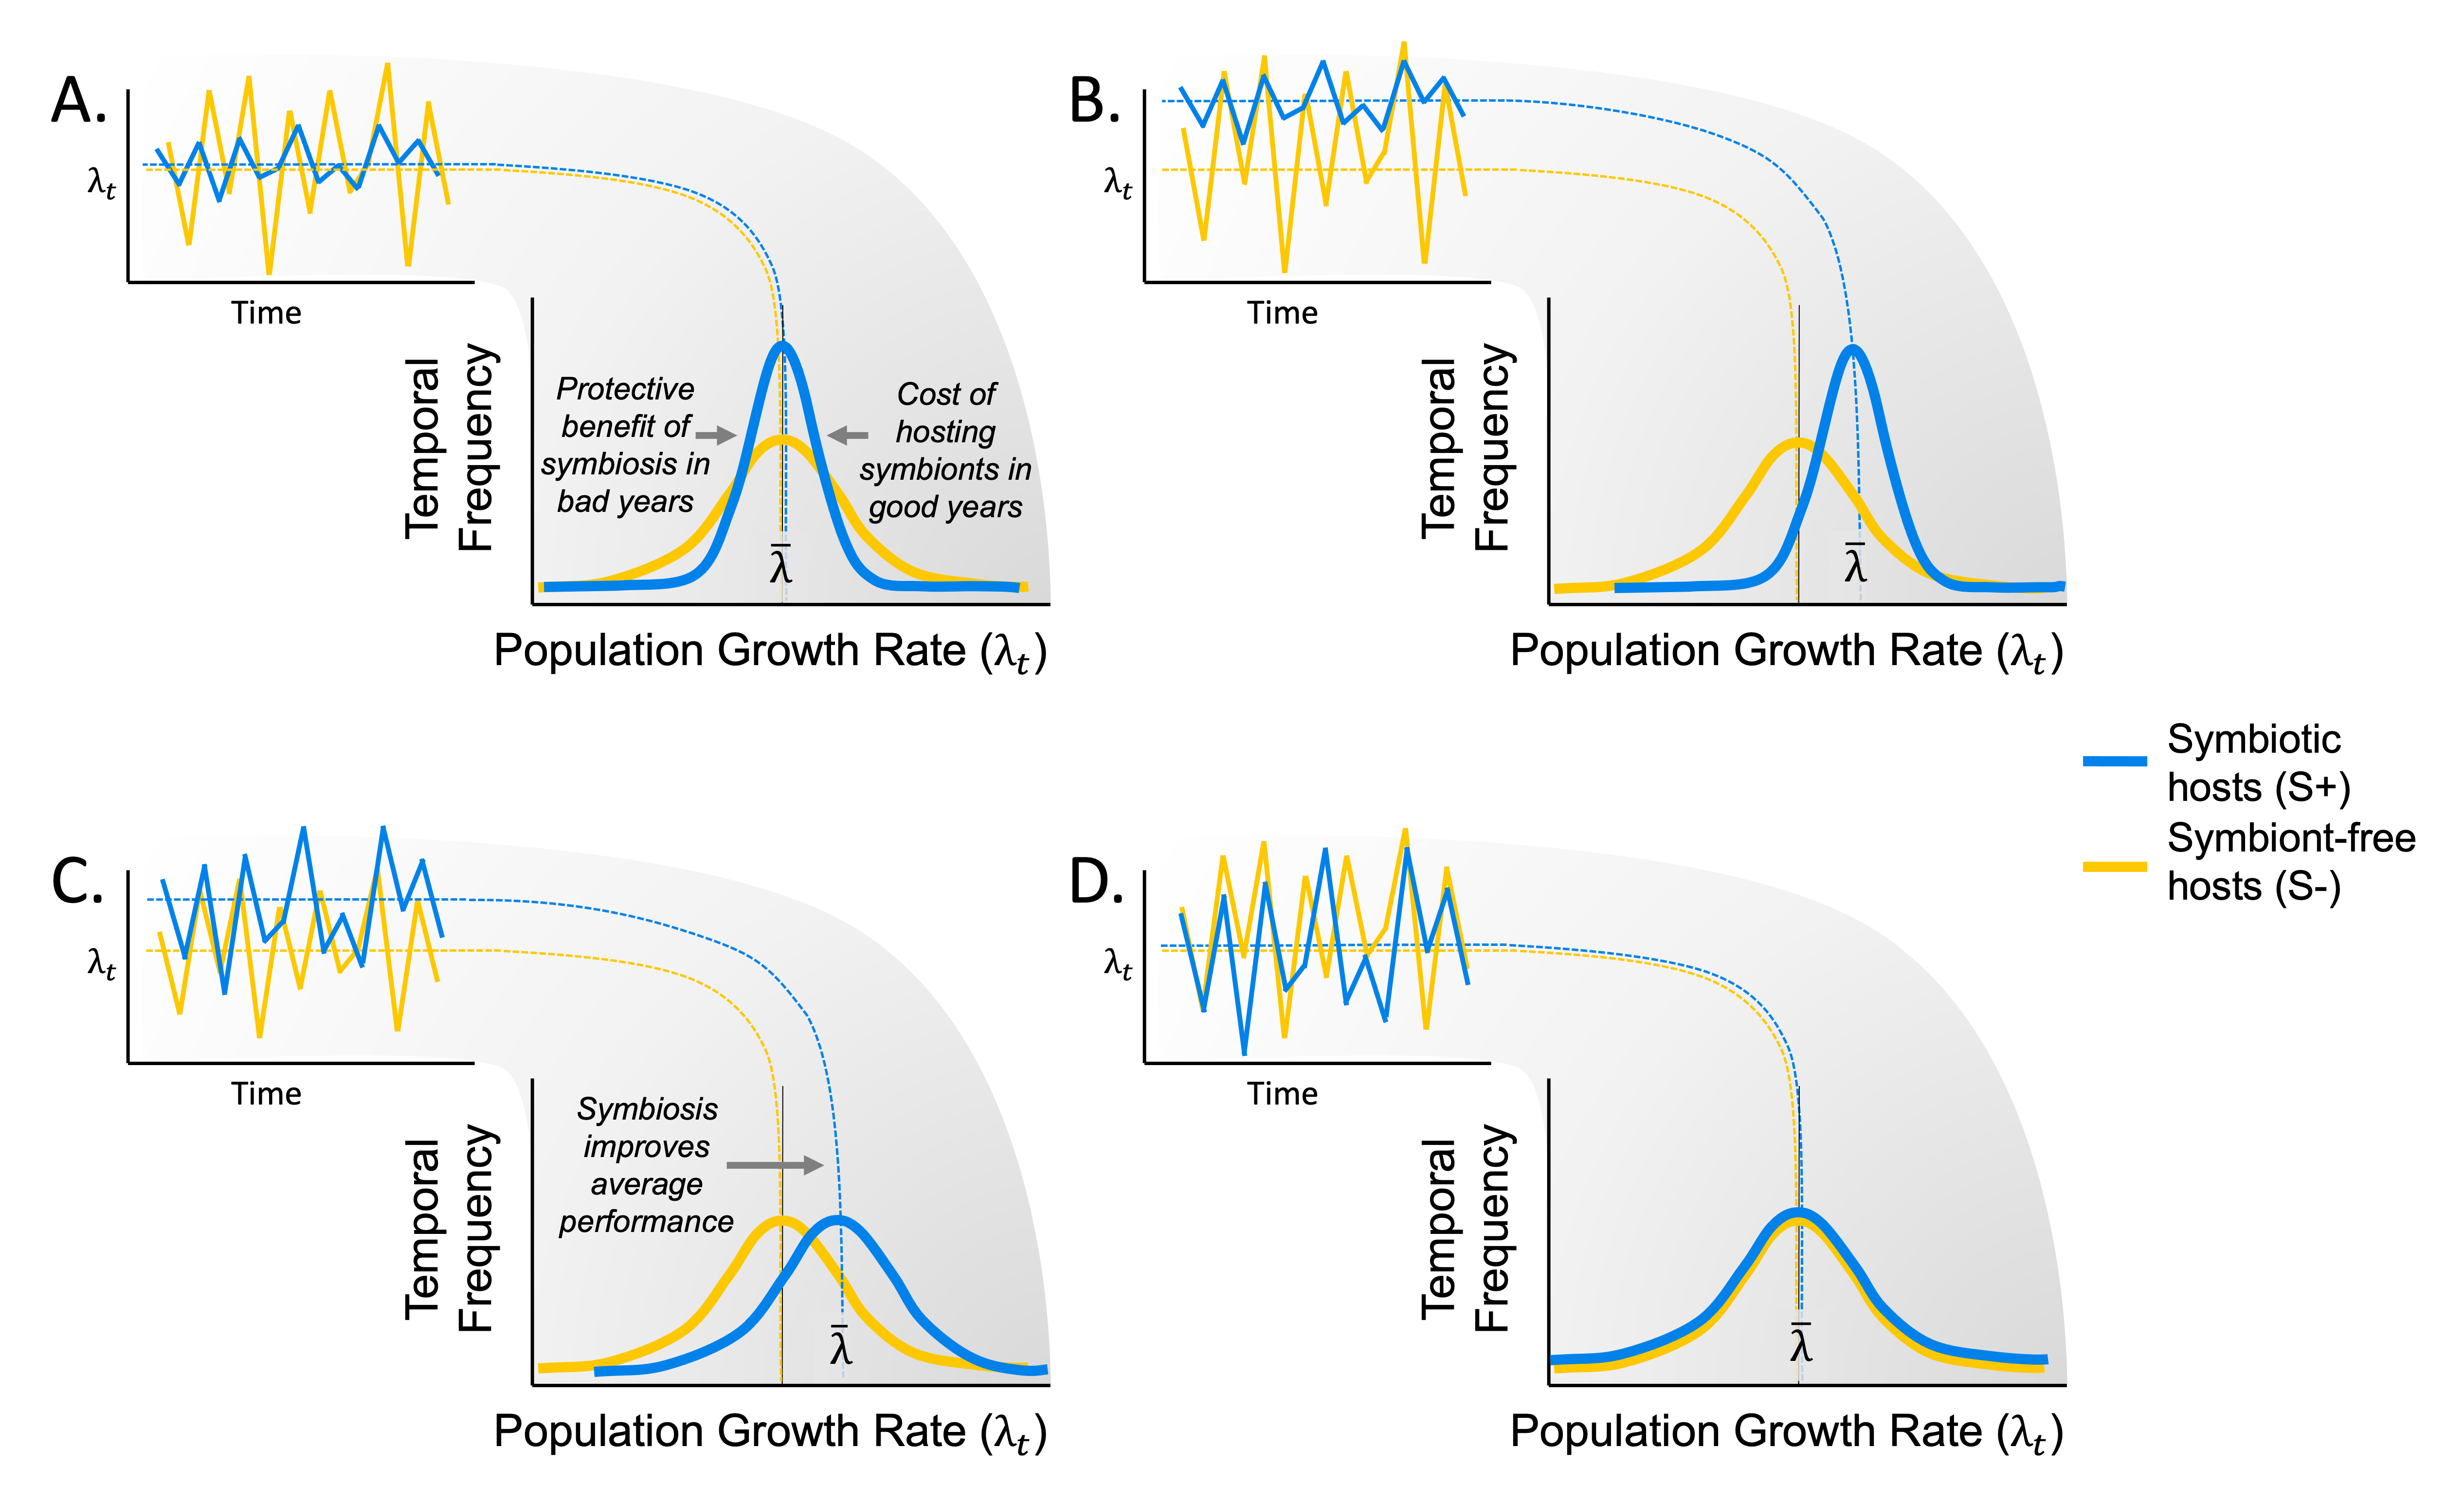
\includegraphics[width=\linewidth]{StochDemo_new_Fig1.png}
	\caption{Hypothesized effects of symbiosis on the mean and variance of annual population growth rates. (A) Context-dependent symbiosis may provide benefits to hosts during harsh years while being neutral or costly during benign years.  Temporal variance in populations growth rates of symbiotic host populations (S+; blue lines) is expected to decrease relative to symbiont-free hosts (S-; yellow lines). (B) Symbiosis may improve average performance across years in addition to reducing temporal variance. (C) Consistent benefits of symbiosis could improve average performance across years with no influence on temporal variance. (D) Symbiosis may have an effectively neutral effect on population growth rates.}
\end{figure*}

\begin{figure*}[h]
	\centering
	\includegraphics[width=\linewidth]{StochDemo_newFig2.png}
	\caption{Endophyte symbiosis altered host vital rates.(A) Shading represents the posterior mean standardized effect size (Cohen's D) of endophyte symbiosis on mean or standard deviation of host vital rates (blue indicates that symbiosis increased the mean or standard deviation and red indicates a reduction). Endophytes' diverse vital rate effects include increased (B) mean growth of \emph{A. perennans} and (C) mean survival probability of \emph{F. subverticillata}. Endophyte presence also reduced inter-annual standard deviation in (D) the survival of \emph{F. subverticillata} and (E) the fertility of \emph{P. alsodes}. In panels B-C, mean vital rate estimates are shown with 80\% credibles along with data binned by size for symbiotic (S+) and symbiont-free (S-) plants, while panels D-E show estimated posterior distributions of endophyte-status specific inter-annual standard deviation ($\sigma^2_{\tau_{e,h}}$)  for each vital rate for S+ (blue) and S- (beige) populations. Organism silhouettes modified from "Festuca subverticillata" by Cindy Roch\'e and "Agrostis hyemalis" and "Poa alsodes" by Sandy Long \copyright Utah State University.}
\end{figure*}

\begin{figure*}
	\centering
	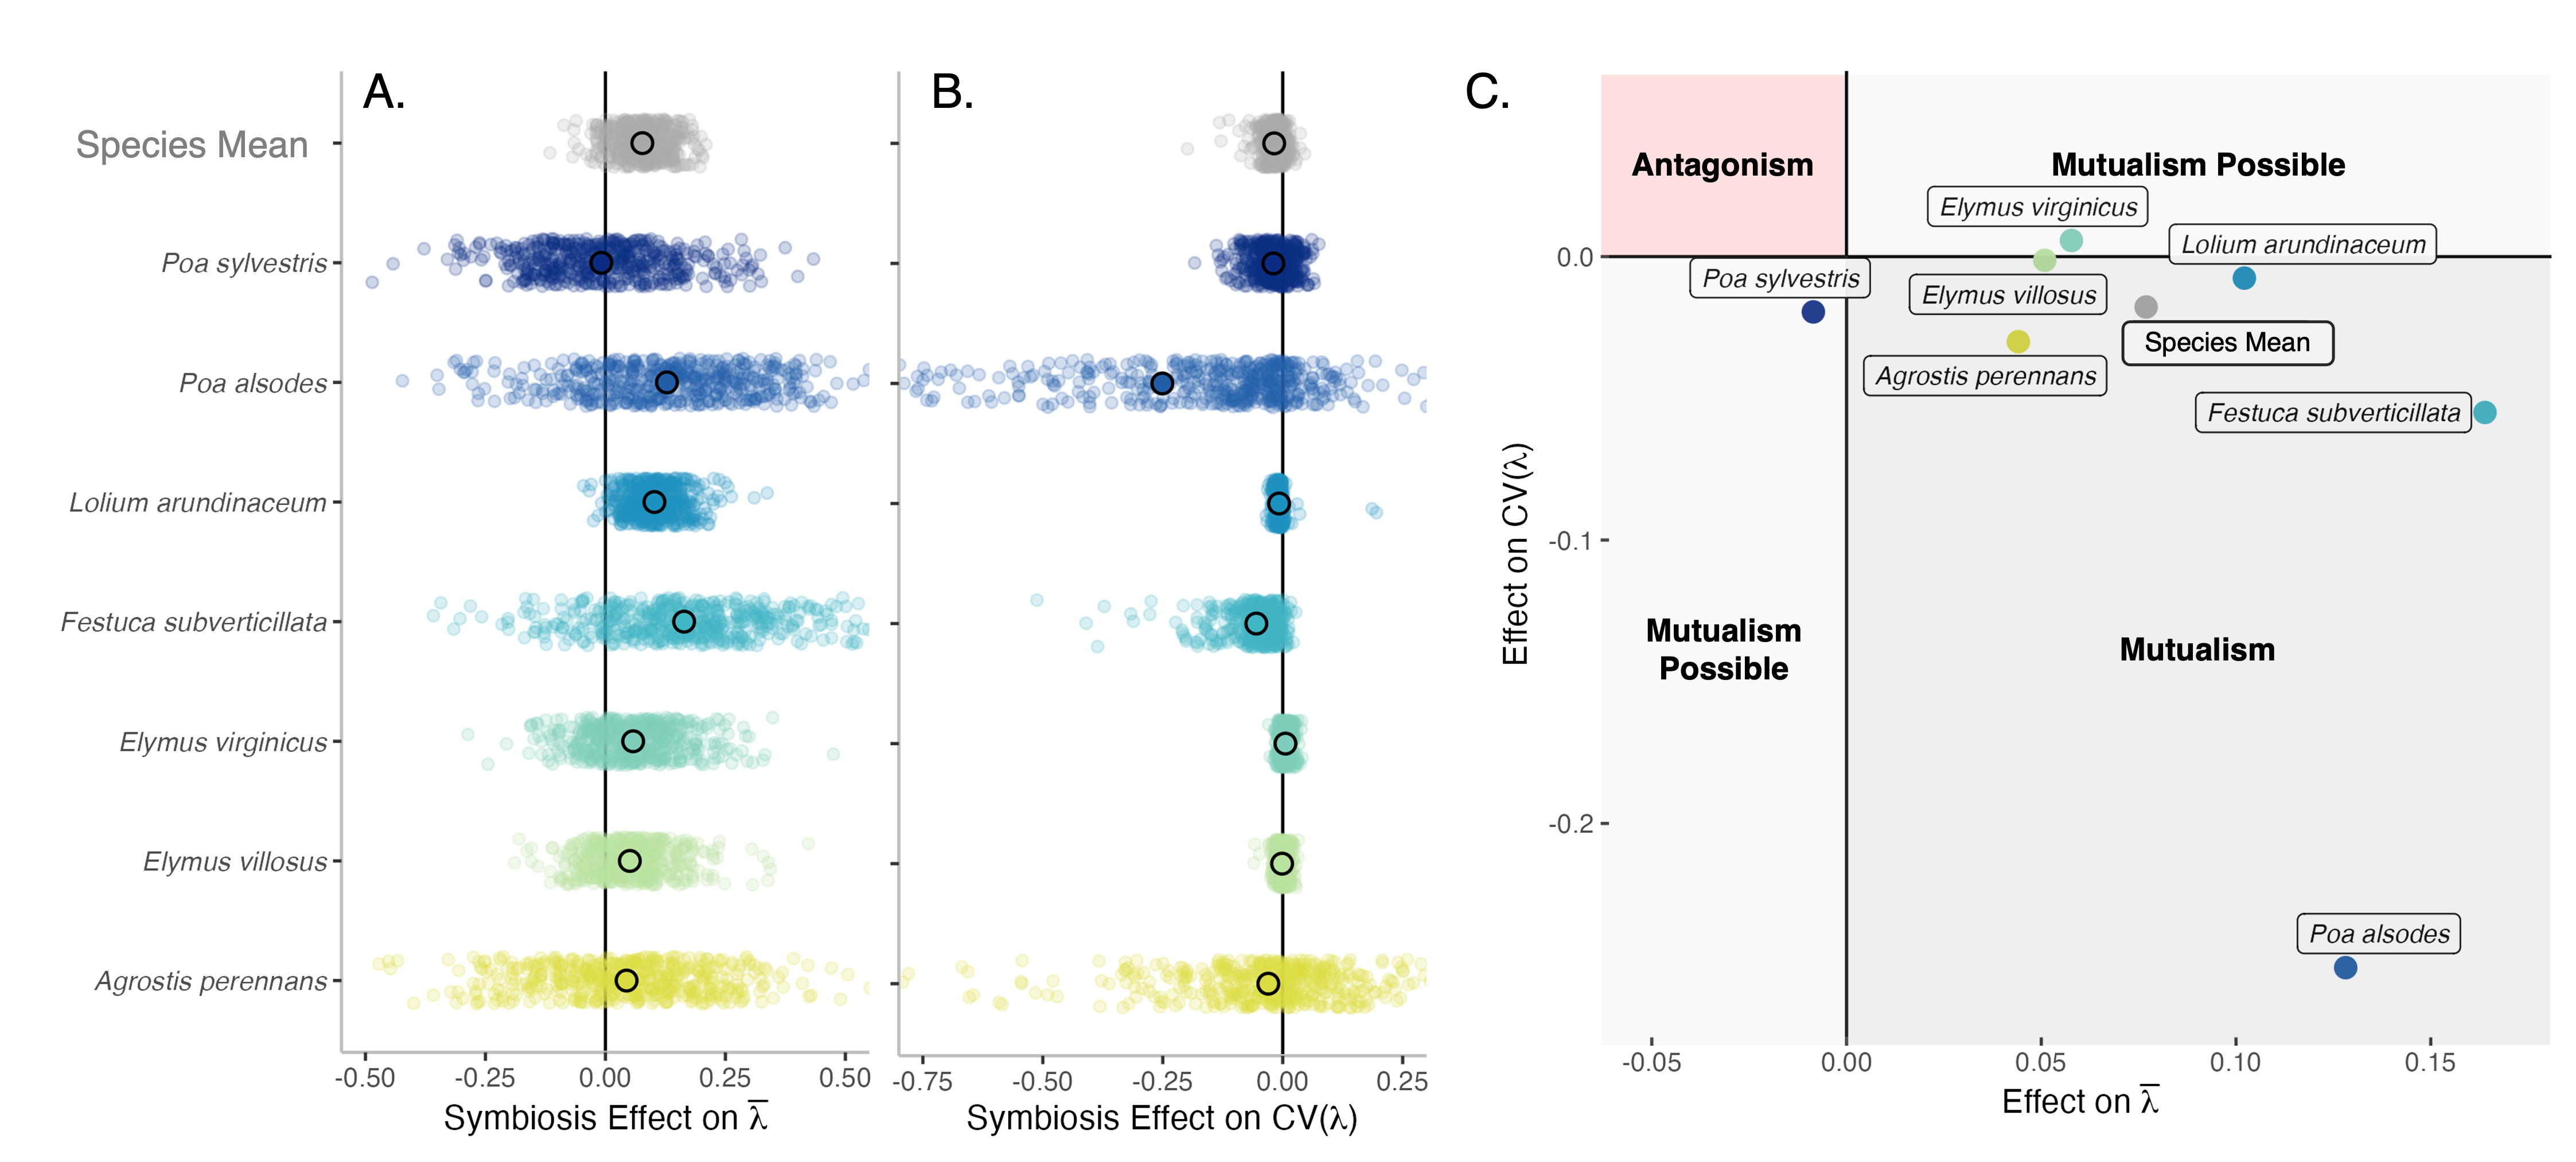
\includegraphics[width =\linewidth]{StochDemo_fig3new.png}
	\caption{Mean and variance-buffering effects on fitness. Black circles indicate the average effect of endophytes along with 500 posterior draws (smaller colored circles) on the (A) mean and (B) coefficient of variation in $\lambda$ for each host species as well as a cross species mean. (C) For all hosts, endophytes either reduce variance, increase the mean, or both, and consequently when considering stochastic environments, the interactions are always at least potentially mutualistic.}
\end{figure*}

\begin{figure*}
	\centering
	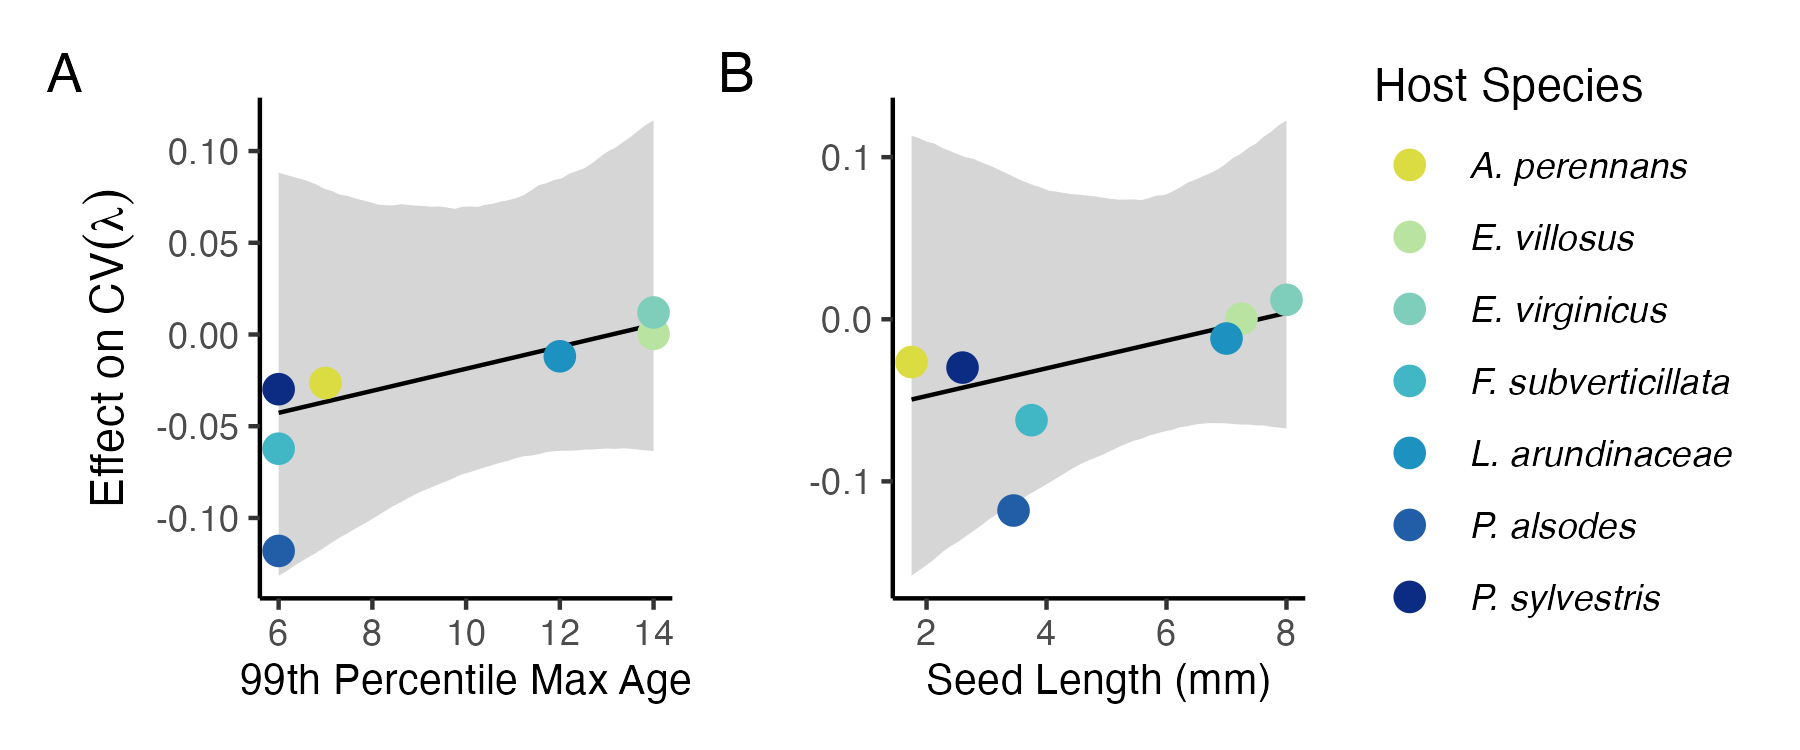
\includegraphics[width=.8\linewidth]{StochDemo_fig4new.png}
	\caption{Host species with faster life history traits experience stronger effects of symbiont-mediated variance buffering. Regressions between life history traits describing the fast-slow life history continuum ((A) 99th percentile maximum age observed during long term censuses in years; (B) Seed size) and the effect of endophyte symbiosis on the coefficent of variation in population growth rate ($\lambda$). Each panel shows the fitted mean relationship (line) along with the 95\% credible interval.}
\end{figure*}

\begin{figure*}
	\centering
	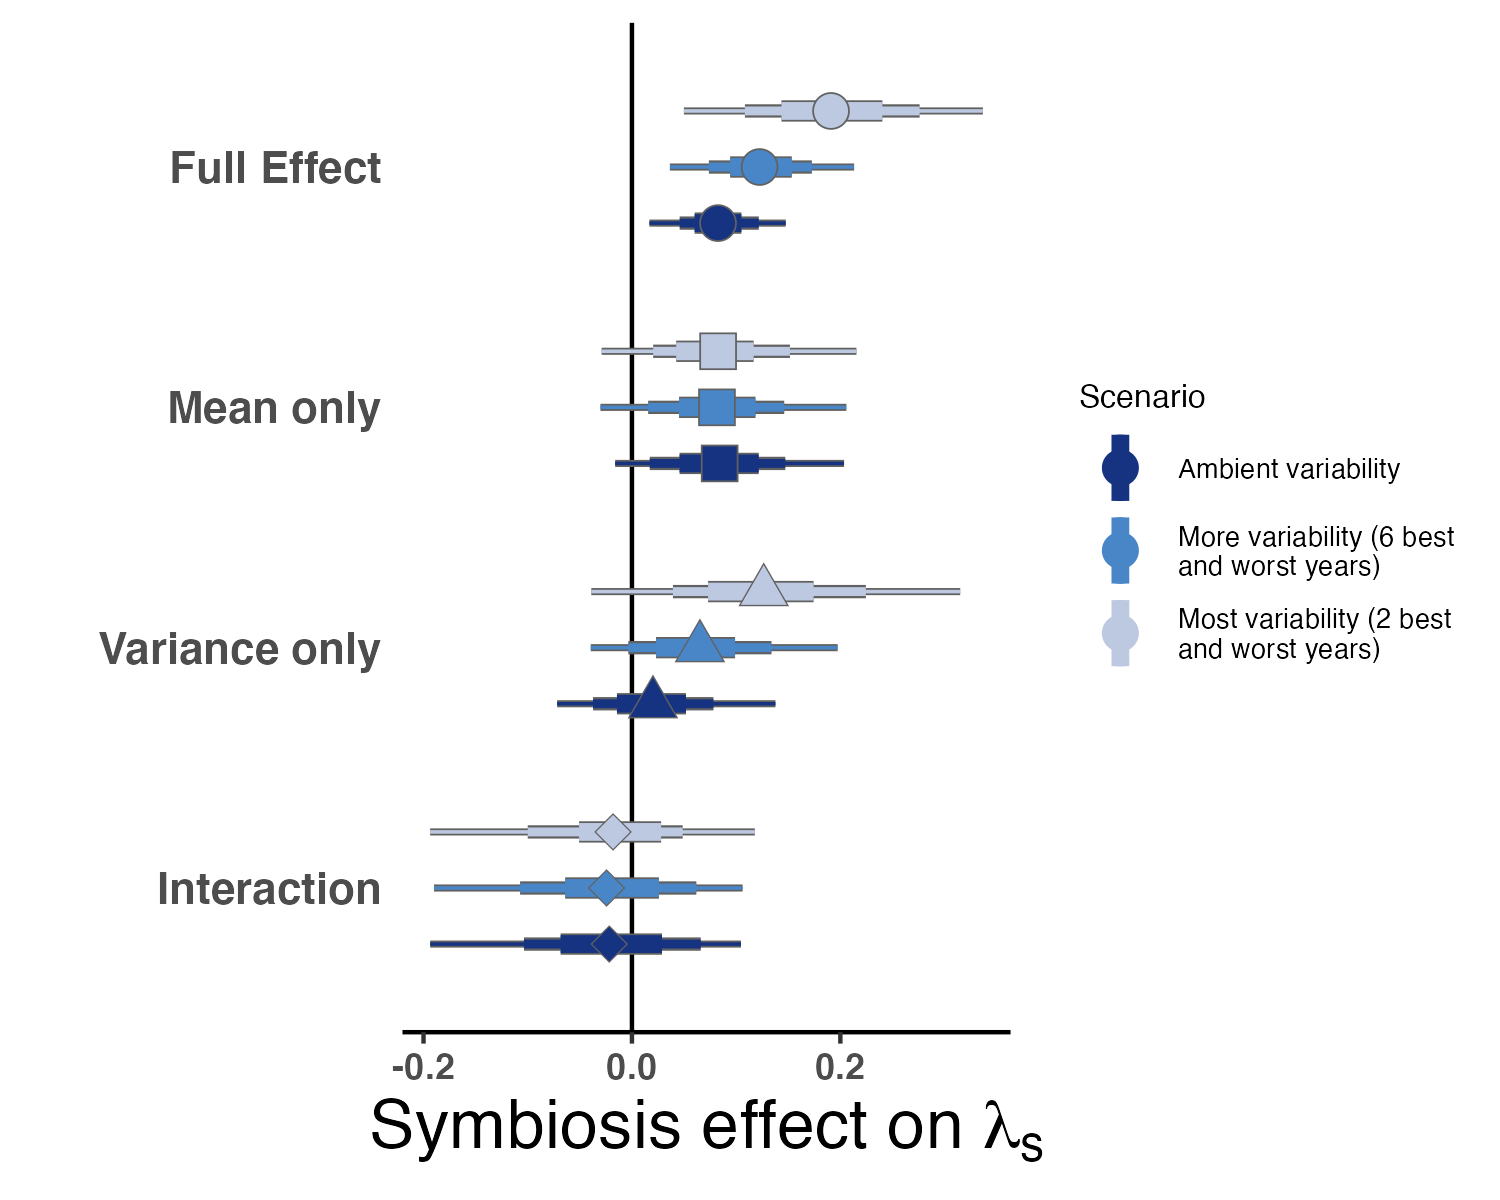
\includegraphics[width=.8\linewidth]{StochDemo_fig5new.png}
	\caption{Cross-species average endophyte contributions to stochastic growth rates under observed and elevated variance. Endophyte symbiosis contributes to the total effect of mutualism on $\lambda_{S}$ through benefits to mean growth rates and through variance buffering as well as the interaction between mean and variance effects. Shapes indicate the posterior mean of each contribution averaged across the seven focal symbiota, along with bars for the 50, 75 and 95\% credible intervals.  The full effect of the symbiosis (circles) becomes more mutualistic under scenarios of increased variance (represented by color shading). Relative to the ambient scenario sampling transition matrices for all 13 transition years during the study period, simulations increased variance by sampling the most extreme six or two years years, leading to increased contributions from variance buffering effects (triangles) and a constant contribution from mean effects (squares).}
\end{figure*}



\clearpage

\begin{appendices}

\section*{Supporting Information}\label{secA}

\subsubsection*{Supplemental Methods}

\subsubsection*{Detailed vital rate modeling}

We fit vital rates models in a Bayesian hierarchical framework. 
Statistical models for adult survival, seedling survival, adult growth, seedling growth, flowering (yes or no), fertility of flowering plants (number of flowering tillers), production of seed-bearing spikelets (number per inflorescence), the average number of seeds per spikelet, and the recruitment of seedlings from the preceding year's seed production, were constructed as follows:

\emph{Survival} - We modeled survival as a Bernoulli process, where the survival ($S$) of an individual $i$ in plot $p$ and census year $t$ was predicted by the plot-level endophyte status ($e$), host species ($h$), size in the preceding census, and the plant's origin status (whether it was initially transplanted or naturally recruited into the plot).

\begin{subequations}
	\label{eq:survival}
	\begin{align}
		S_{i,p,e,h,t} \sim Bernoulli(\hat{S}_{i,p,e,h,t})\\
		logit(\hat{S}_{i,p,e,h,t}) = \beta_{0_{h}} + \beta_{1}*origin_{i}\\
		+ \beta_{2_{h}}*endo_{e} + \beta_{3_{h}}*size_{i,t-1} + \tau_{e,h,t} + \rho_{p}\\
		\tau_{e,h,t} \sim Normal(0,\sigma^2_{\tau_{e,h}})\\
		\rho_{p} \sim Normal(0,\sigma^2_{\rho})
	\end{align}
\end{subequations}

Here, $\hat{S}$ is the survival probability, $\beta_{0_{h}}$ is an intercept specific to each host species, $\beta_1$ is the effect of the plant's recruitment origin, $\beta_{2_{h}}$ is the endophyte effect, $\beta_{3_{h}}$ is the size effect, $\tau_{e,h,t}$ is a normally distributed year effect for each species and endophyte status with variance $\sigma^2_{\tau_{e,h}}$, and $\rho_{p}$ is a normally distributed plot effect with variance $\sigma^2_{\rho}$ ($p(e)$ indicates that plot identity is uniquely associated with an endophyte status).
We assume that origin effect $\beta_1$ and plot-to-plot variance $\sigma^2_{\rho}$ are shared across host species, allowing us to ``borrow strength'' across the multi-species dataset; other model parameters are unique to host species. 
We separately modeled the survival of newly recruited seedlings with a similar model but omitting previous size dependence and origin status. 
%All random effects were estimated independently between seedling and adult vital rates models.


\emph{Growth} - We modeled plant size in census year $t$ ($G$) with the same linear predictor for the mean as described for survival.
Because we measured size as positive integer-valued counts of tillers, we modeled it with a zero-truncated Poisson-inverse Gaussian distribution.
This distribution includes a shape parameter $\lambda_G$ to account for overdispersion in the data.
We additionally modeled the growth of newly recruited seedlings separately with a Poisson-inverse Gaussian model omitting size structure and the plants' origin status as with seedling survival.

\emph{Flowering} - We modeled whether or not a plant was flowering during the census ($P$) as a Bernoulli process, with the same linear predictor for the mean as described above for survival except that size dependence for reproductive vital rates was determined by the individual's size during the same census year as opposed to its size during the previous year.

\emph{Fertility} - For a plant that was flowering during the census, its fertility was the number of reproductive tillers produced ($F$), which we modeled as a function of size in the same census period with a zero-truncated Poisson-Inverse Gaussian distribution, with the same linear predictor for the mean as described above. 

\emph{Spikelets per Inflorescence} - Spikelet production ($K$) was recorded as integer counts on up to three inflorescences per reproducing plant.
We modeled these data with a negative binomial distribution, with the same linear predictor for the mean as described above. 

\emph{Seed Production per Spikelet} - For individuals with recorded counts of seed production, we calculated the number of seeds per spikelet from our counts of seeds and spikelets per inflorescence, and then modeled seeds per spikelet ($D$) as means of a Gaussian distribution for each species and endophyte status. 
Because we had less detailed data across years and plants for seed production than for other reproductive vital rates, we omitted both plot and year random effects. 

\emph{Seedling Recruitment} - We used a binomial distribution to model the recruitment of new seedlings ($R$) into the plots from seeds produced in the preceding year, assuming no long-lived seed bank. 
We included an intercept specific to each host and endophyte status and the same random effects structure as in other models. 
We estimated the number of seeds per plot in the preceding year by multiplying the total number of reproductive tillers per plant by the mean number of spikelets per inflorescence and mean number of seeds per spikelet ($D$).
For plants with missing fertility or spikelet data, we used the expected number of reproductive tillers ($F$) or of spikelets per inflorescence from ($K$), drawing from the full posteriors of our models. 
We rounded this value to get the estimated seed production for each individual, and finally summed across all reproductive plants in each year and plot to get the total number of seeds produced. 


\subsubsection*{Estimating climate drivers of environmental context-dependence}{

	To connect the variance buffering effects of endophytes with inter-annual variability in climate, we built climate-explicit stochastic matrix population models from the vital rate data in addition to the climate-implicit model described in the main text. 
	Identifying the potentially complex relationships between vital rates and environmental drivers remains a key challenge for accurate forecasts of the ecological impacts of environmental stochasticity \cite{ehrlen2015predicting}.
	We first downloaded temperature and precipitation data from a weather station in Bloomington, IN,  approx. 27 km from our study site, using the rnoaa package \cite{chamberlain2022package}. 
	Compared to other weather stations in the area, the measurements from Bloomington contain the most complete climate record across the study period and are correlated with more local measurements from Nashville, IN for years in which local data are available (total daily precipitation: $R^2$ = .76; mean daily temperature: $R^2$ = .94).
	The mean annual temperature across the study period was 11.9 $C^o $ (SD: 1.05 $C^o $) and the average annual precipitation was 1237.9 mm/year (SD: 204.89 mm/year) (Fig. S24).
	Given the known role of endophytes in promoting host drought tolerance, we calculated the Standardised Precipitation-Evapotranspiration Index (SPEI) for 3 and 12 months preceding each annual censuses, reflecting drought during the growing season and across the year \cite{vicente2010multiscalar}.
	To calculate SPEI, we used the Thornthwaite equation to model potential evapotranspiration as implemented in the SPEI R package \cite{begueria2013spei}
	
	We repeated the process of fitting statistical models for each vital rate as described in \textbf{Materials and Methods} with the inclusion of a parameter describing the influence of SPEI. 
	We fit separate vital rate models incorporating either the growing season or annual drought index for each vital rate, except for the model describing the mean number of seeds per inflorescence. 
	This model was fit without climate effects because the data came from only a few years.
	Initial analyses indicated similar fits for models including only a linear term and those with both linear and quadratic terms describing the relationship between the climate driver and the vital rate response, and so we proceeded with models including only the linear term.
	We expected that including climate predictors into the models would explain some inter-annual variance in vital rates, shrinking the variance associated with the fitted year random effects.
	We assessed model fit with graphic posterior predictive checks and convergence diagnostics as described for the climate-implicit analysis. 
	Finally, we next built matrix projection models incorporating the climate-dependent vital rate functions to assess the response of symbiotic (S+) vs symbiont-free (S-) populations to drought. 
	The model is as described in \textbf{Materials and Methods} with the inclusion of parameters describing the slope of the relationship with SPEI. 
	We compared the sensitivity of $\lambda$ to either annual or seasonal SPEI of S+ populations ($\frac{\Delta\lambda^{+}}{\Delta SPEI}$) with those of S- populations ($\frac{\Delta\lambda^{-}}{\Delta SPEI}$)(Fig. S25; Table S).
	
	Most species were slightly more responsive to growing season rather than annual drought conditions, and for most species symbiotic populations were less sensitive to SPEI than symbiont-free populations (Fig. S25; Table S3).
	However, these drought indices did not explain the full extent of inter-annual variability in demographic vital rates.
	For example, flowering in \emph{A. perennans} had one of the strongest climate signals ($82\%$ probability of a positive relationship with SPEI), yet the estimated inter-annual variance $\sigma^2_{\tau_{P}}$ for symbiont-free plants shrank from 6.7 to 6.1 after including 3-month SPEI as a covariate, suggesting that other factors contribute to inter-annual variability.
}

\subsubsection*{Vital rate mean-variance decomposition}{
	We repeated the mean-variance decomposition to quantify the extent that mean and variance effects on stochastic population growth rates arise through different vital rates. 
	Specifically, we repeated the calculation of $\lambda_s$ as described in the main text for symbiotic populations as well as symbiont-free populations, as well as for four additional ``treatments". 
	These treatments differentiate between mortality and growth related vital rates (adult survival, adult growth, seedling survival, and seedling growth) and reproductive vital rates (probability of flowering, inflorescence production, spikelet production, seed production, and recruitment). 
	Each treatment held vital rate mean and interannual variances at the S- reference level across vital rates while introducing (1) endophyte effects on the vital rate means for survival and growth vital rates only, (2) endophyte effects on the vital rate variances for survival and growth vital rates only, (3) endophyte effects on the vital rate means for reproductive vital rates only, and (4) endophyte effects on the vital rate variances for reproductive vital rates only.
	
	The combination of all six $\lambda_s$ treatments allowed us to quantify to what extent the overall effect of symbiosis derives from changes in mean and variance of mortality and growth versus in reproductive vital rates. 
	To explore how these contributions could be expected to change under increased variability relative to that observed during the study period, we repeated this decomposition under the scenarios of increased variance described in the main text, sampling transition matrices associated with the set of either six or two most extreme $\lambda$ values.

	This analysis revealed that both mean and variance buffering effects are driven primarily by symbiont effects on survival and growth rather than on reproduction (Fig S53) .
}
\newpage

\subsection*{Supplemental Figures S1-S28}\label{secS_figs}

\renewcommand\thefigure{S\arabic{figure}}   
\begin{figure}[H]
	\centering
	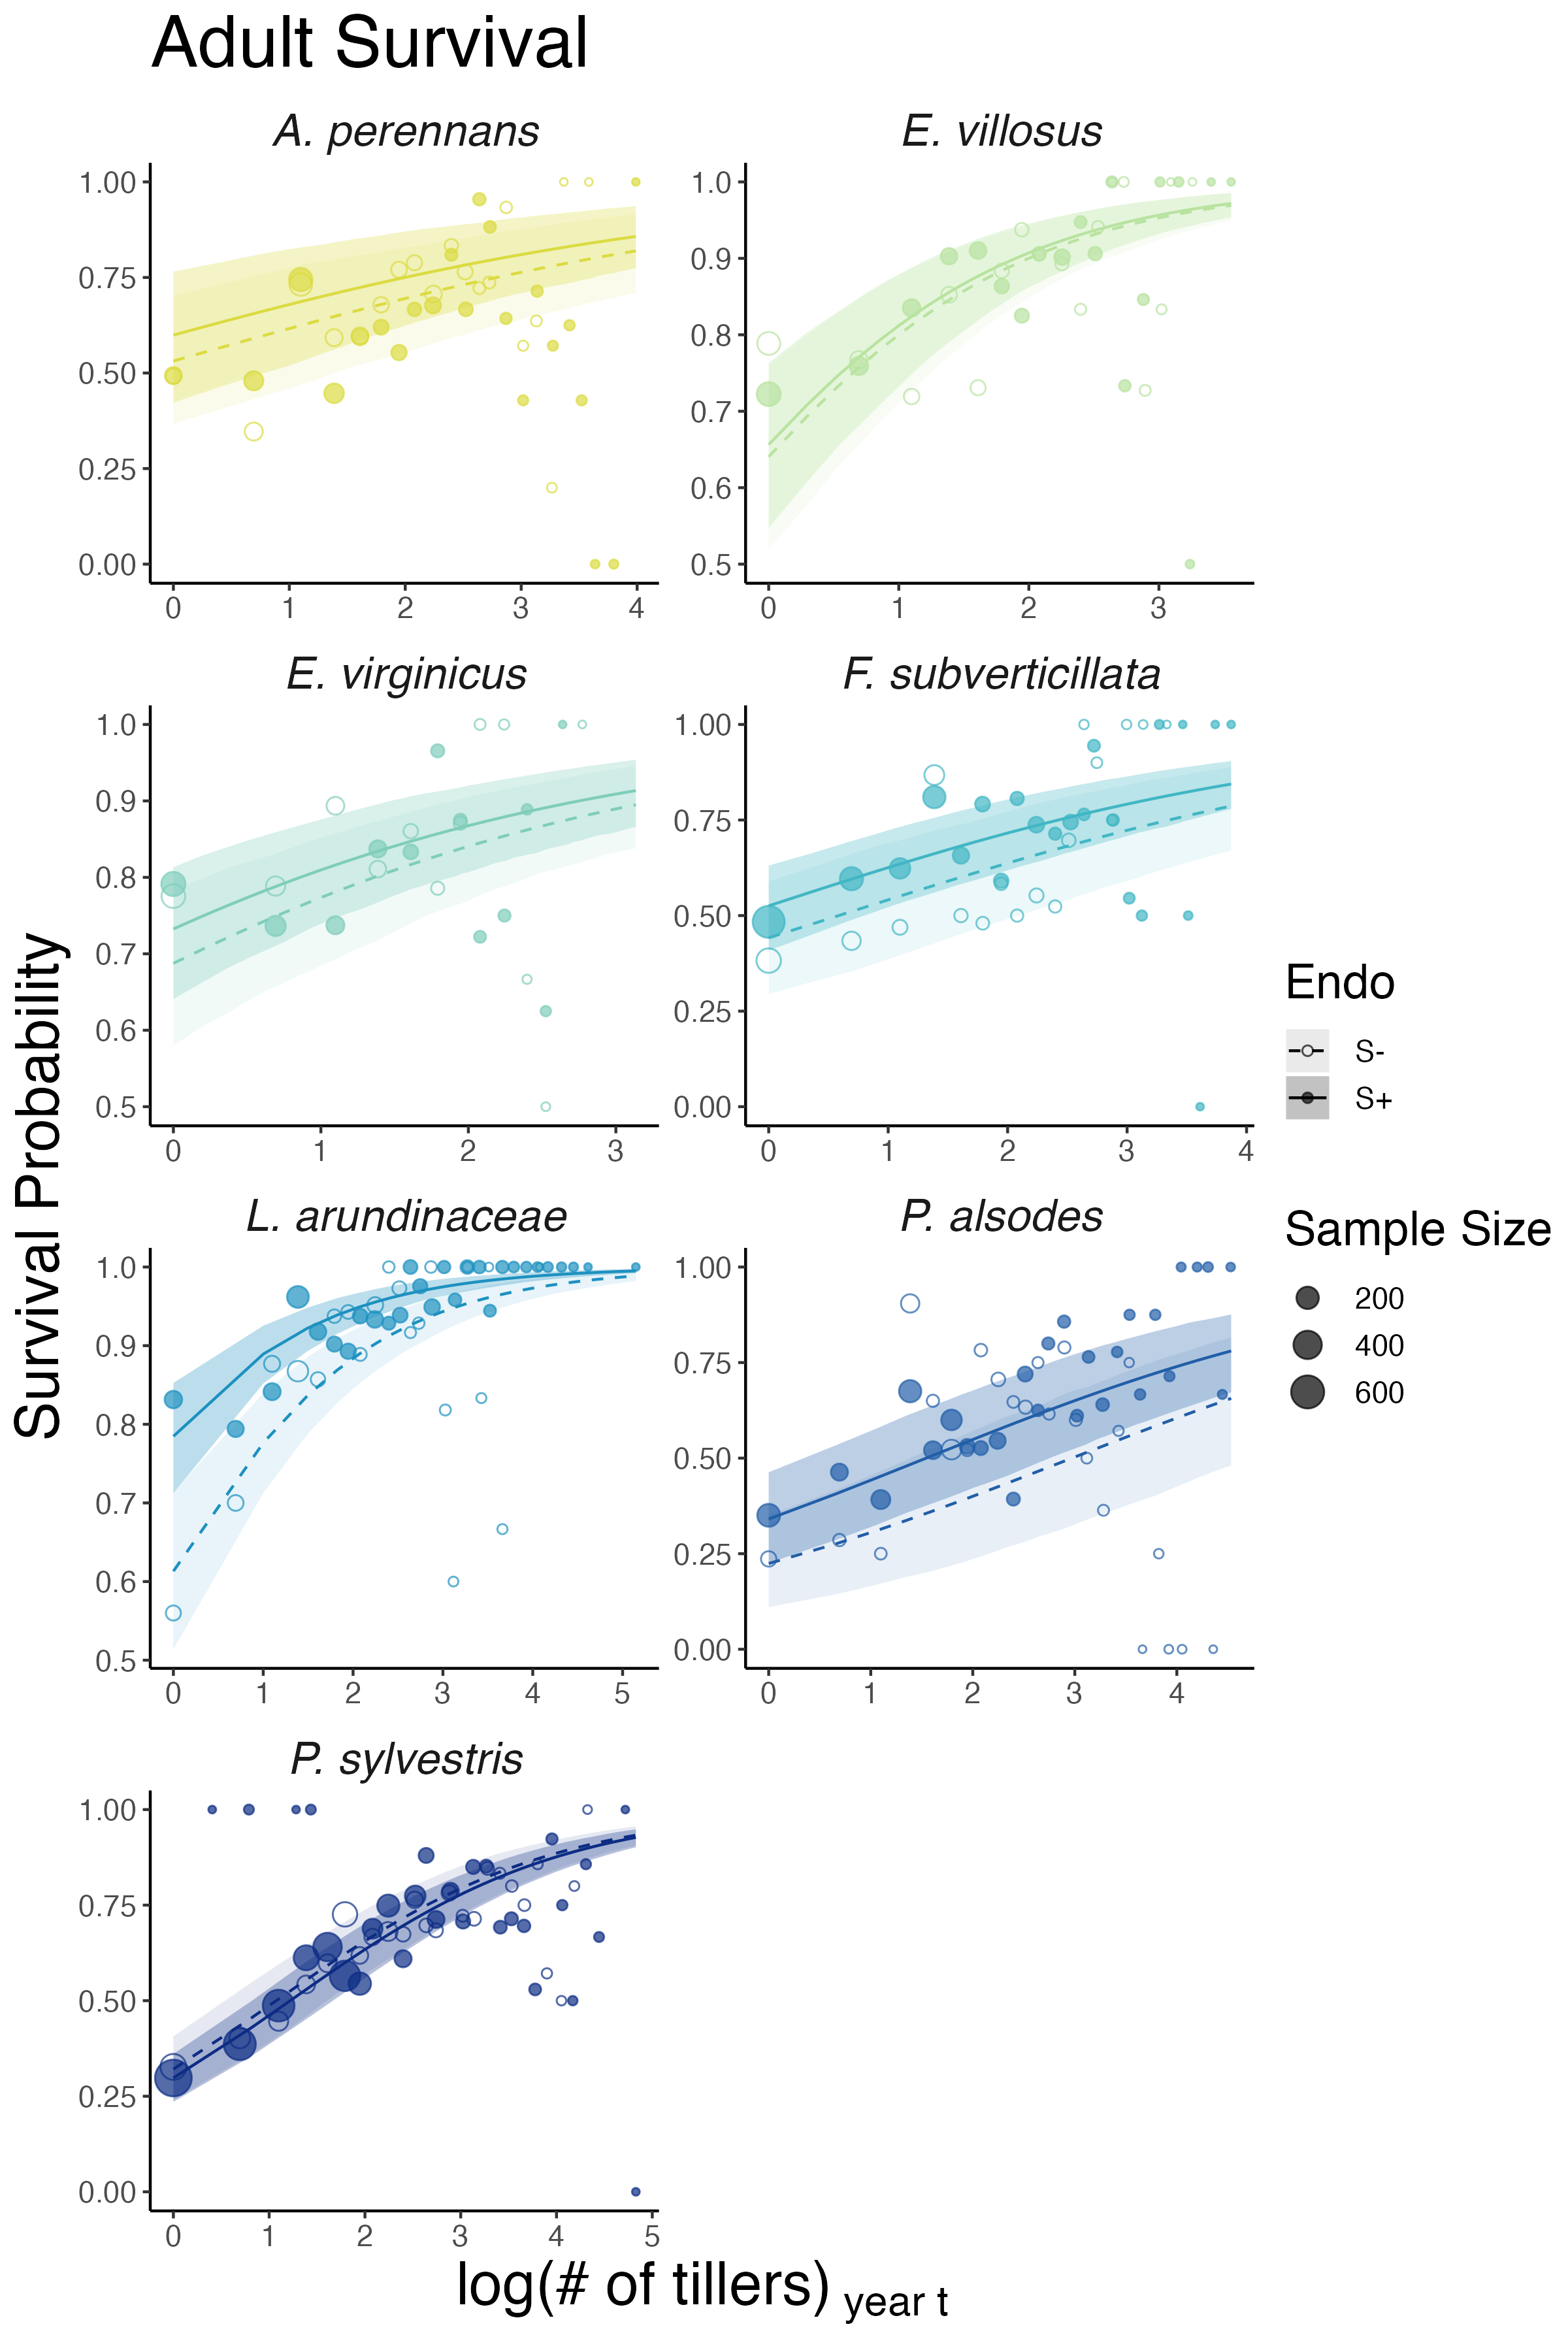
\includegraphics[width=.6\linewidth]{surv_meanplot.png}
	\caption{Effect of endophyte symbiosis on mean adult survival. Fitted curves represent the size-specific mean survival probability for original plants along with data binned by size shown as open circles with a dashed line for symbiont-free (S-) plants, while the solid line and filled circles represent symbiontic (S+) plants. 80\% credible intervals are shown with dark shading for  S+, or light shading for S-.}
\end{figure}
\begin{figure}[H]
	\centering
	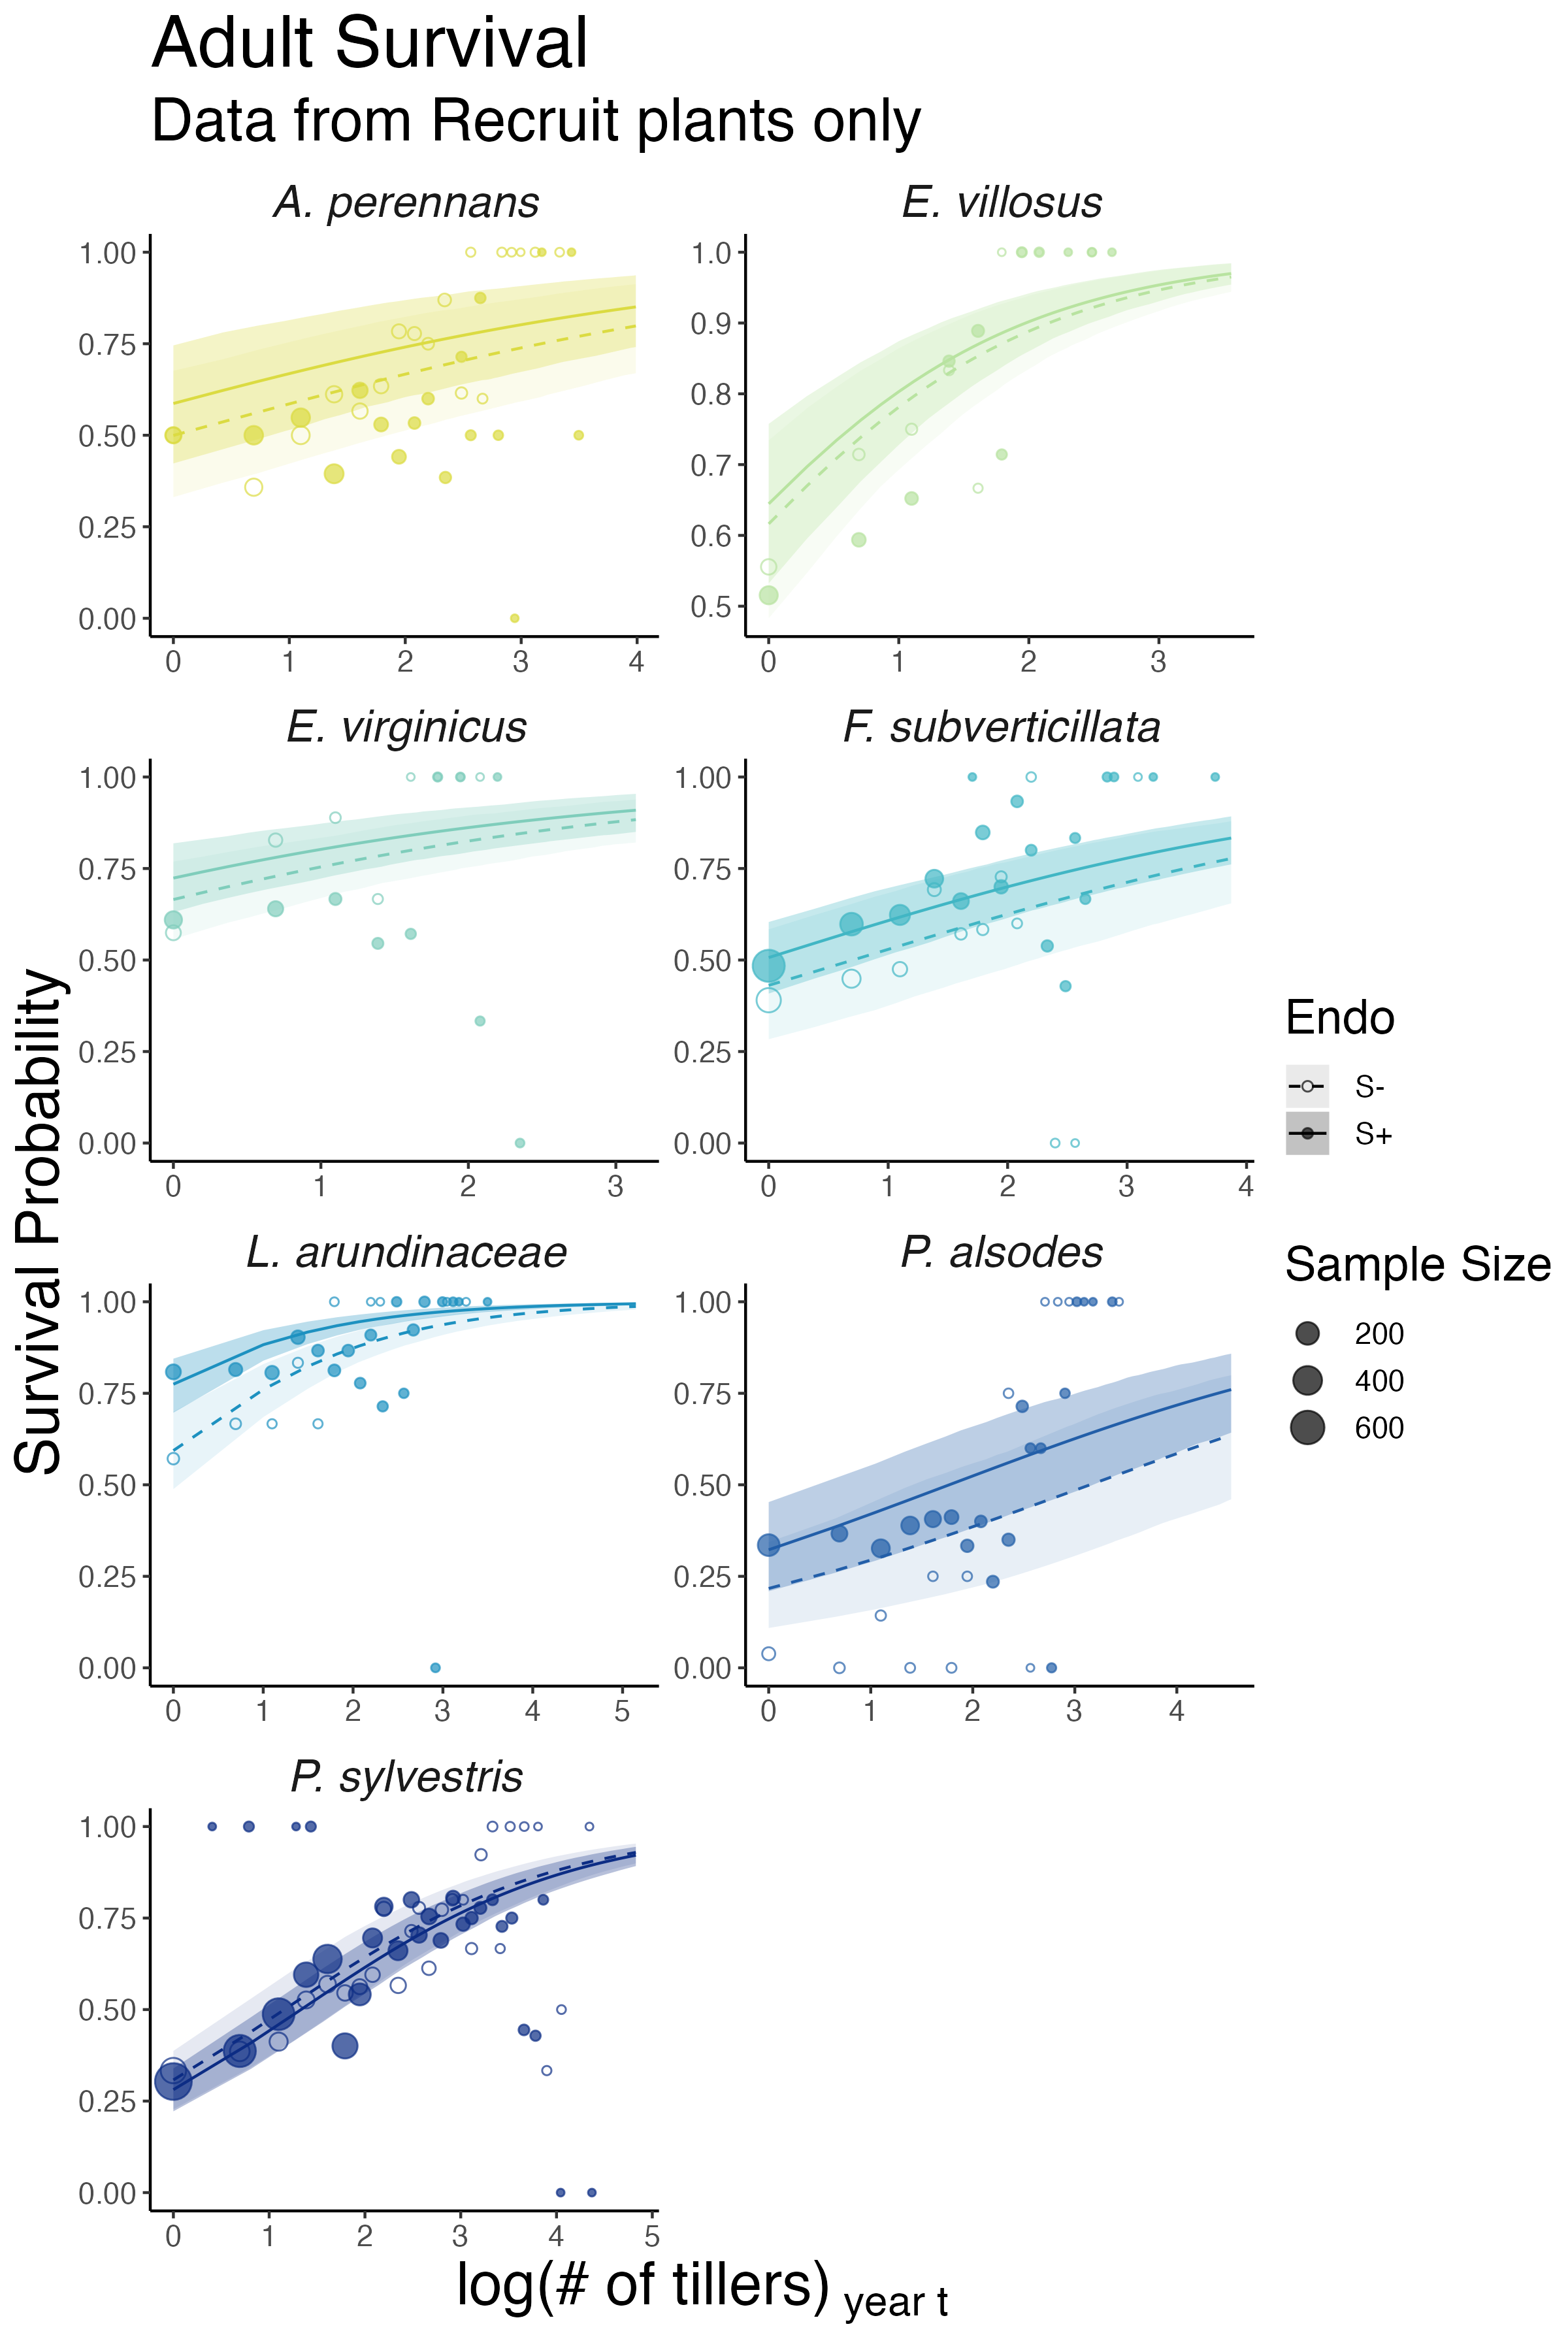
\includegraphics[width=.6\linewidth]{recruit_surv_meanplot.png}
	\caption{Effect of endophyte symbiosis on mean adult survival. Fitted curves represent the size-specific mean survival probability for recruited plants along with data binned by size shown as open circles with a dashed line for symbiont-free (S-) plants, while the solid line and filled circles represent symbiontic (S+) plants. 80\% credible intervals are shown with dark shading for  S+, or light shading for S-.}
\end{figure}

\begin{figure}[H]
	\centering
	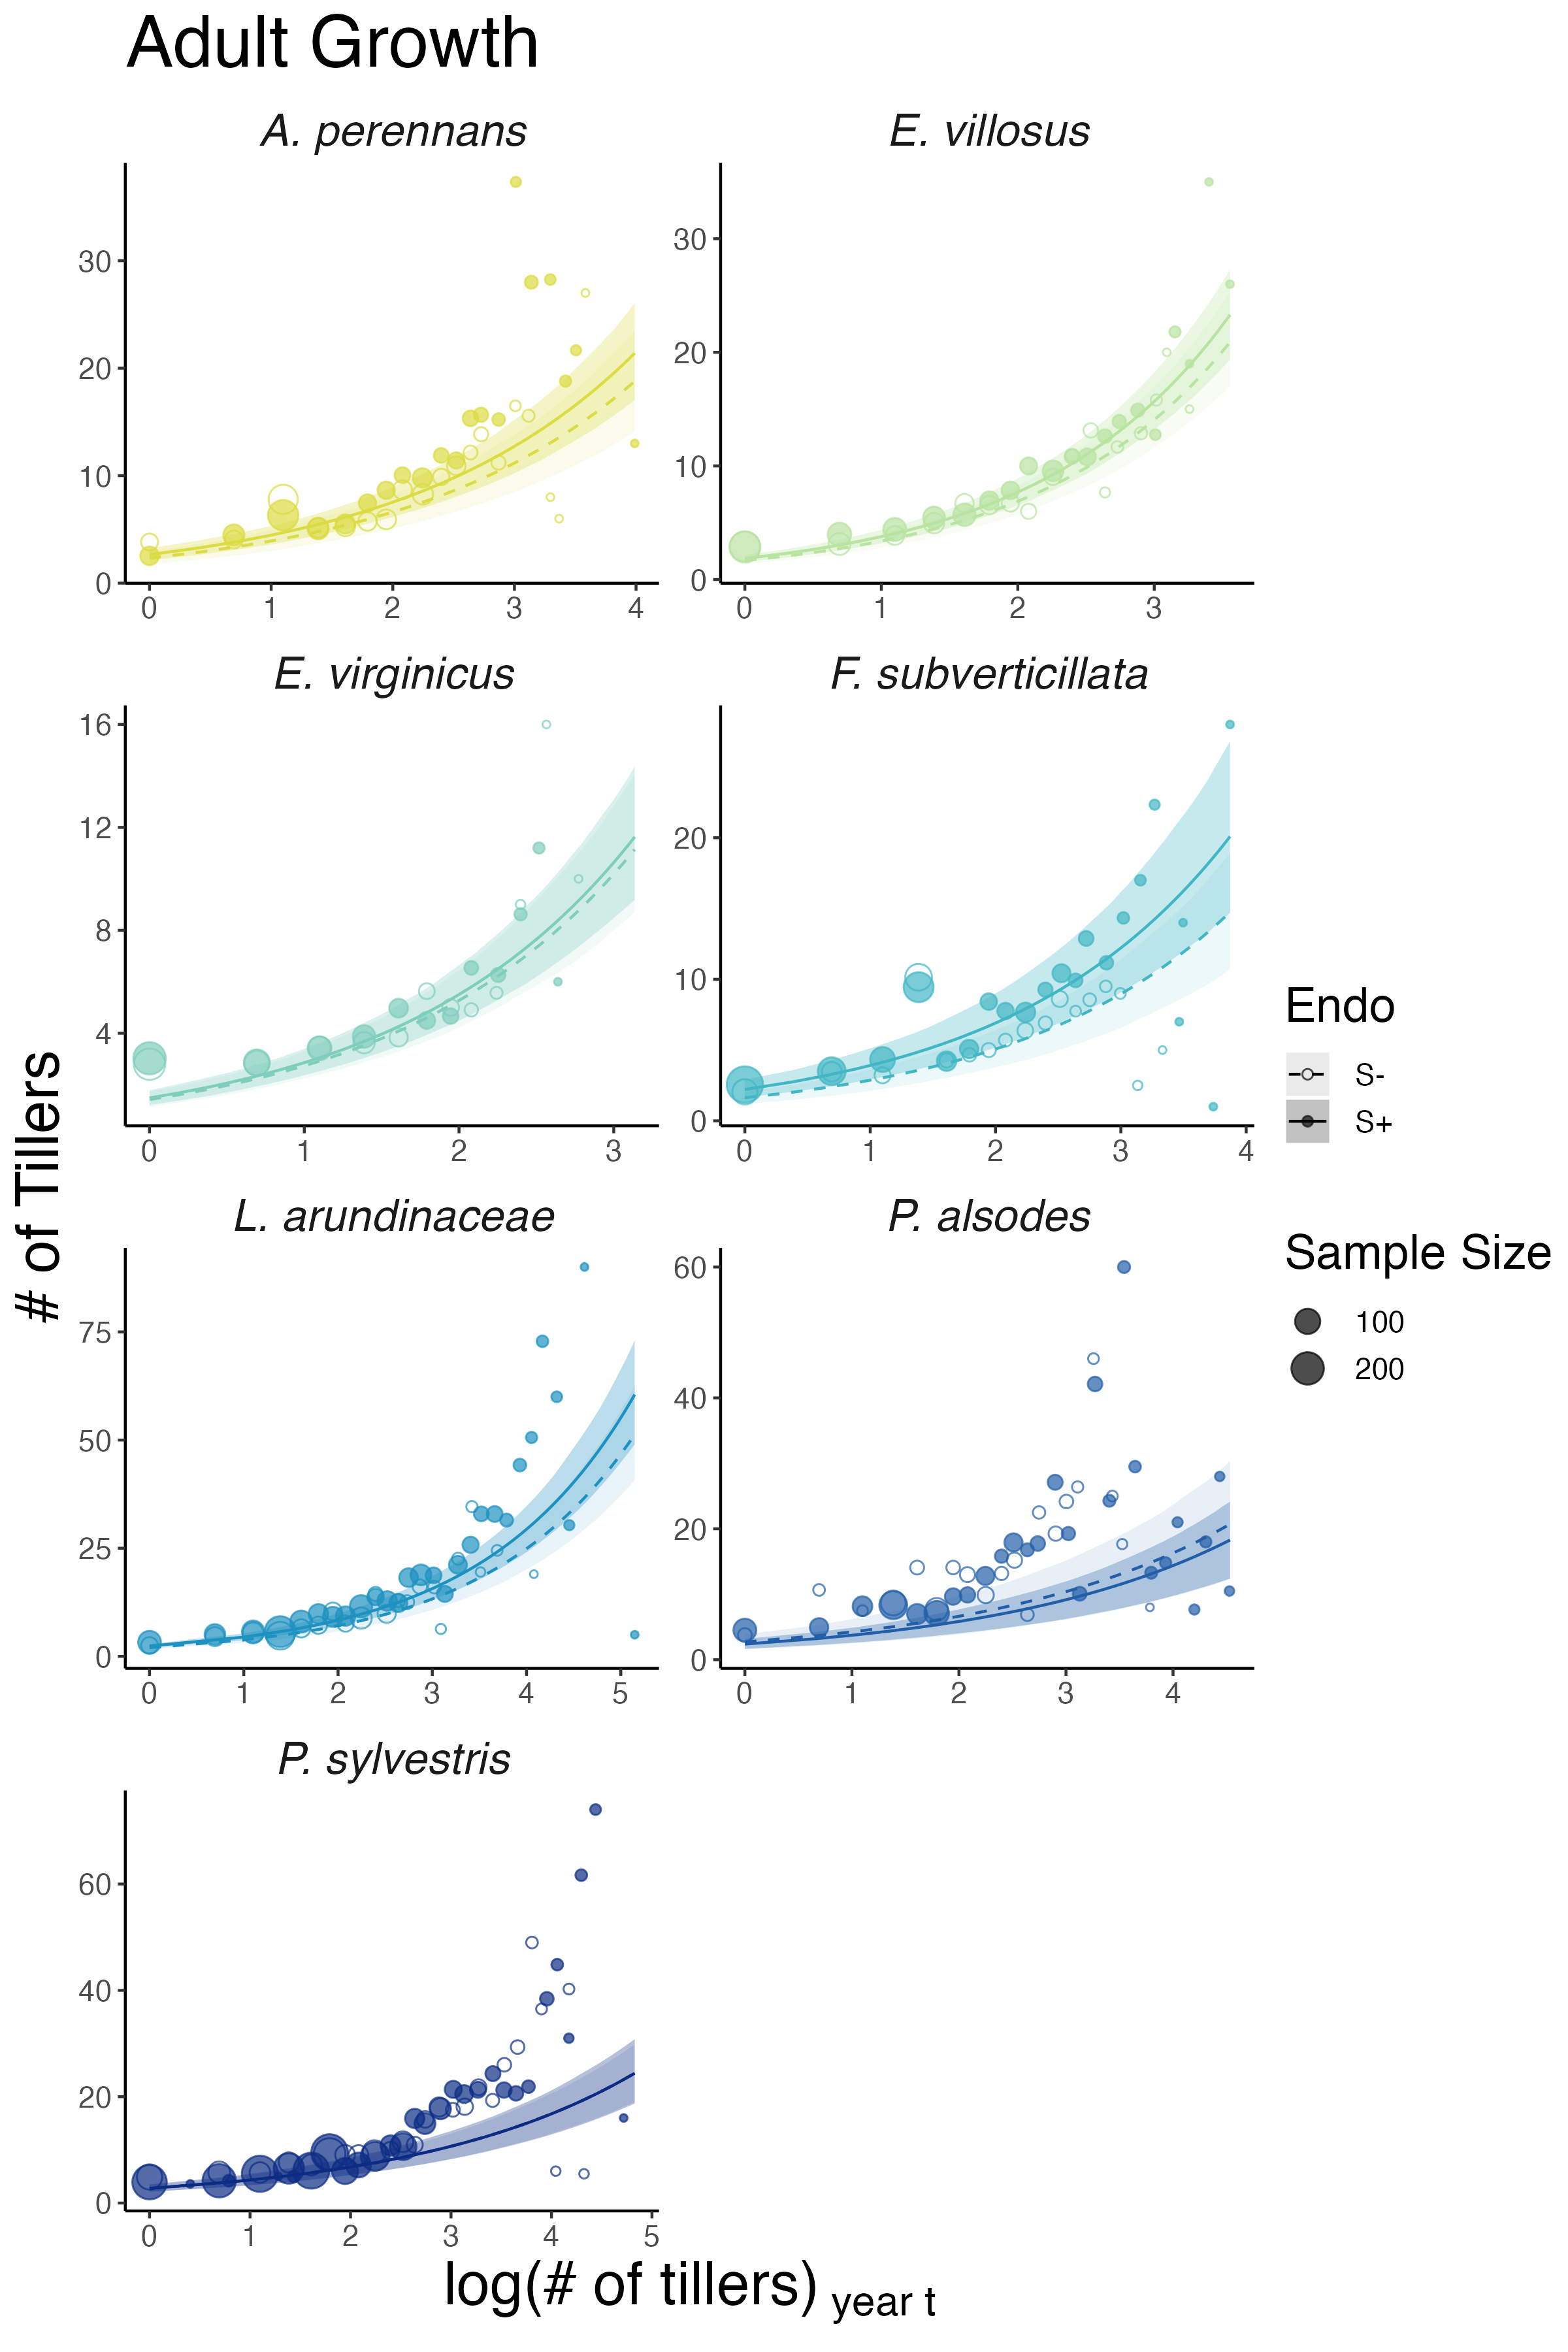
\includegraphics[width=.6\linewidth]{grow_meanplot.png}
	\caption{Effect of endophyte symbiosis on mean adult growth. Fitted curves represent the size-specific mean expected plant size for original plants along with data binned by size shown as open circles with a dashed line for symbiont-free (S-) plants, while the solid line and filled circles represent symbiontic (S+) plants. 80\% credible intervals are shown with dark shading for  S+, or light shading for S-.}
\end{figure}


\begin{figure}[H]
	\centering
	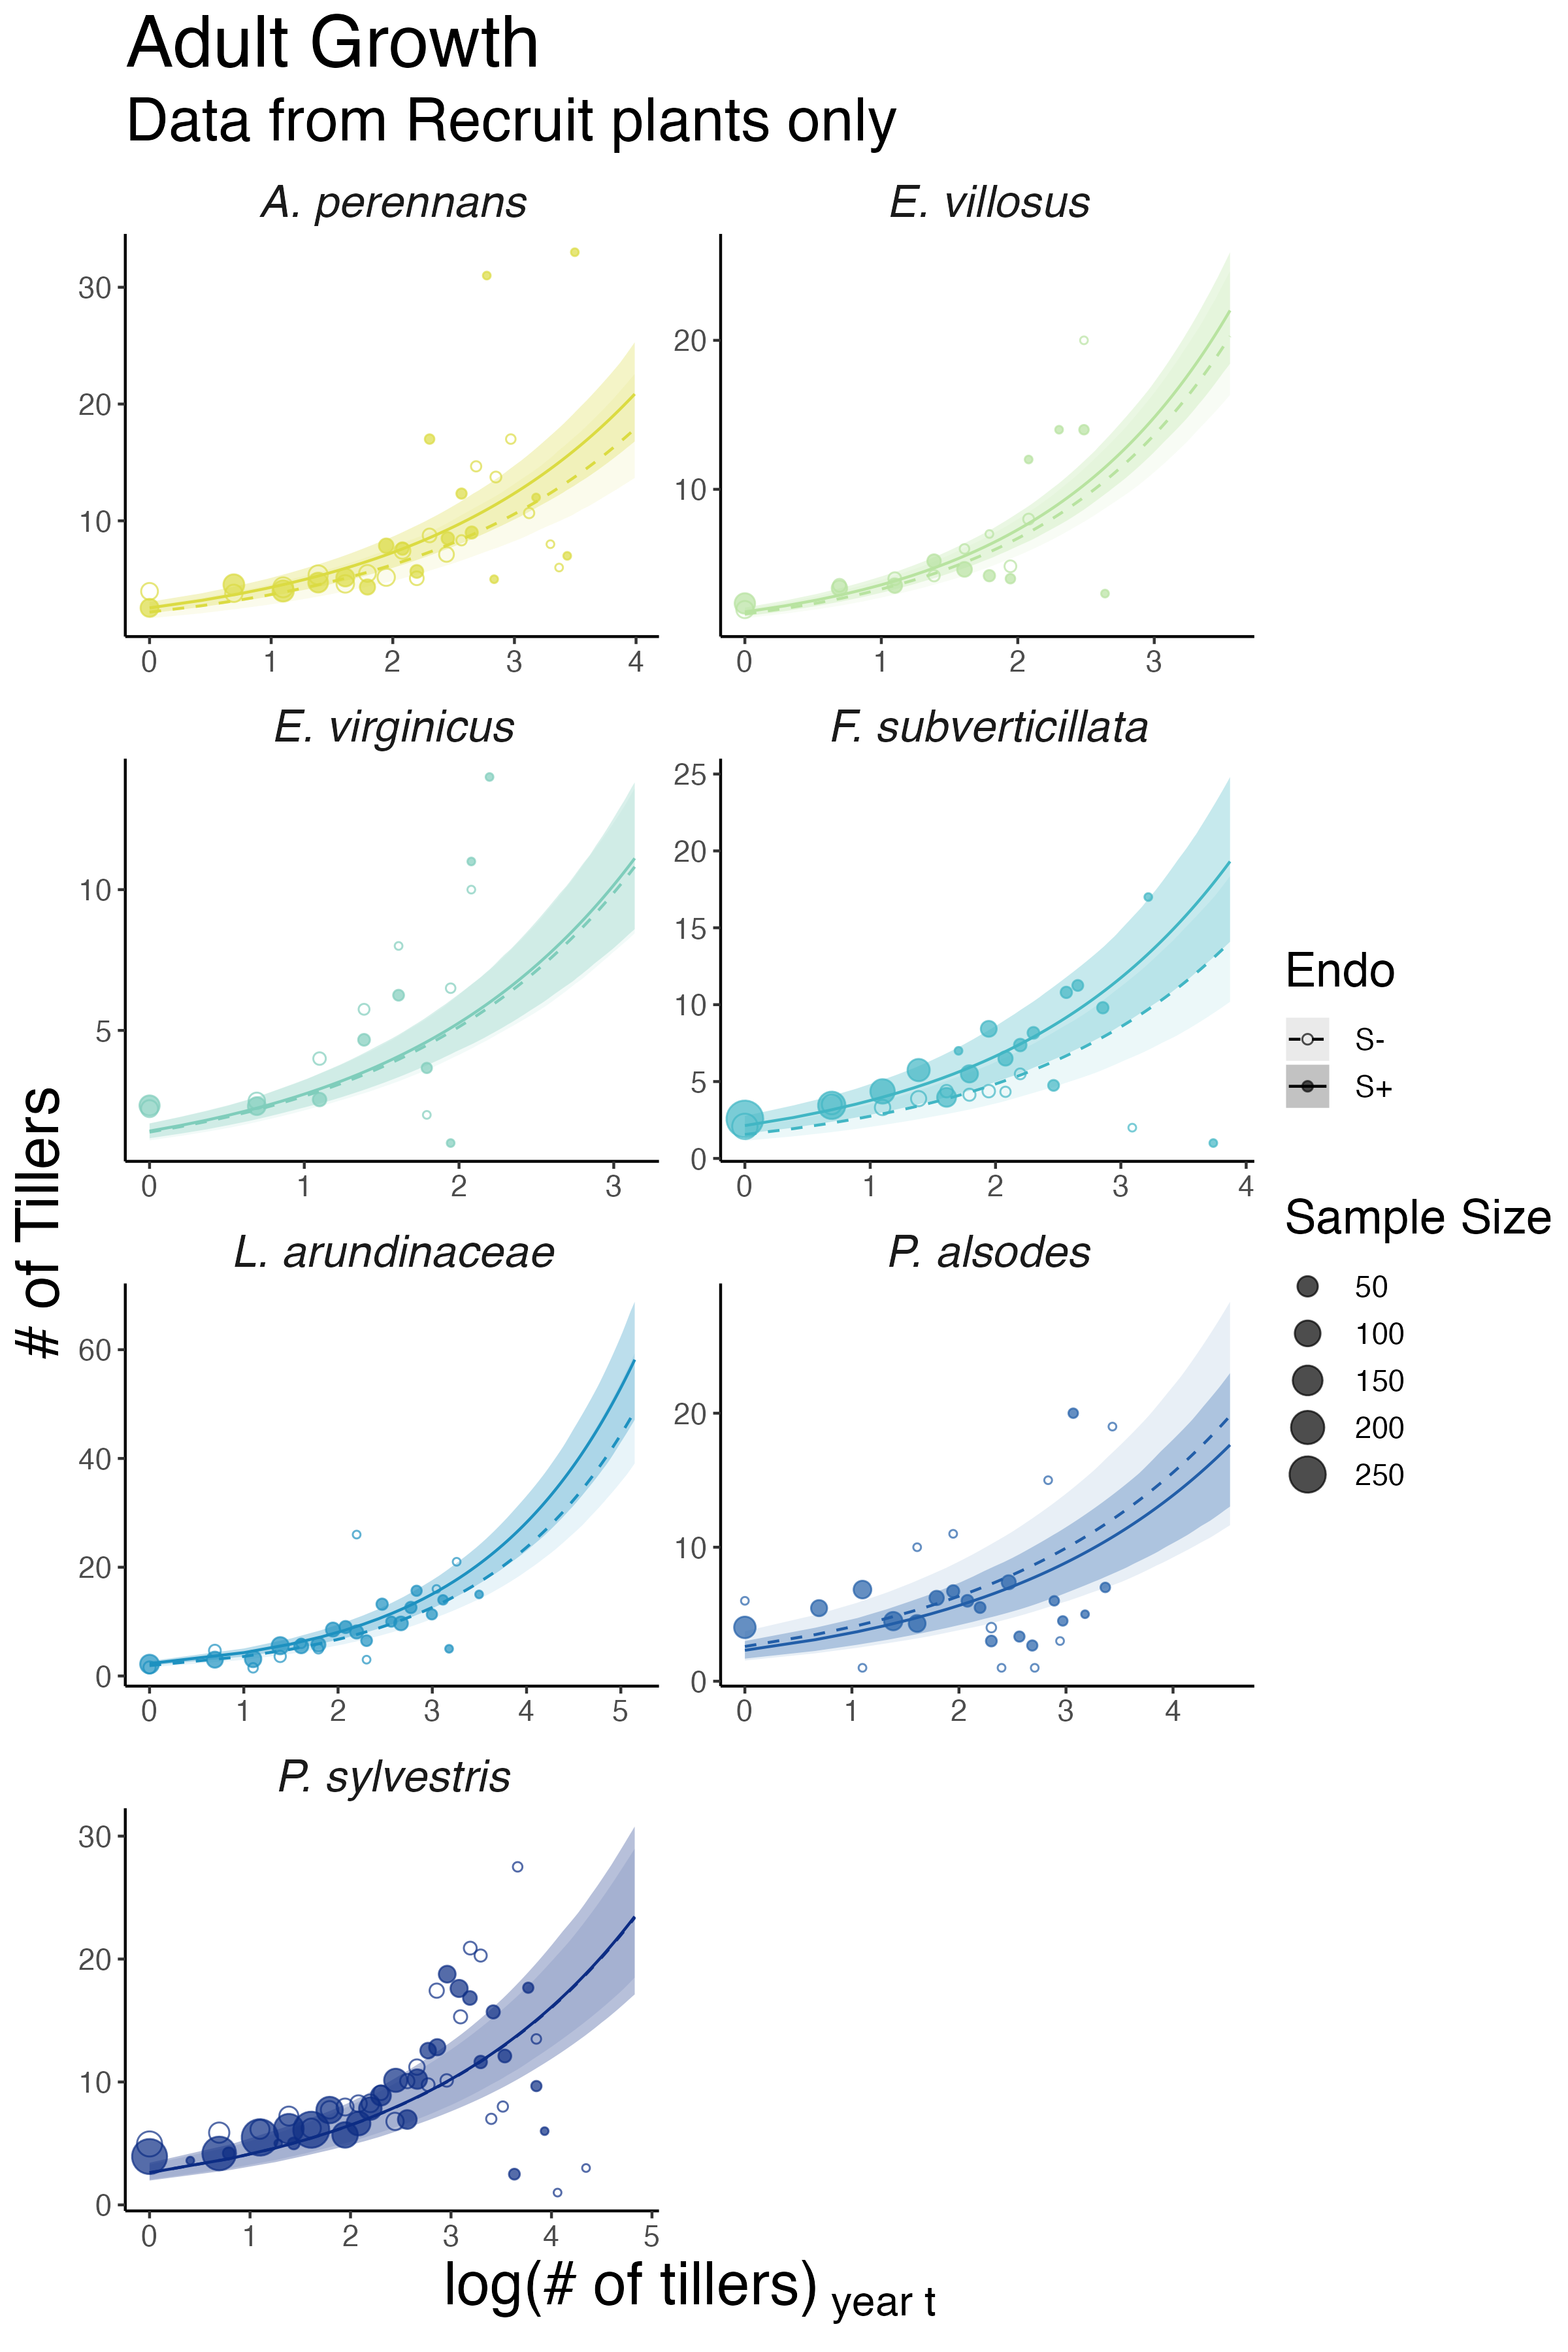
\includegraphics[width=.6\linewidth]{recruit_grow_meanplot.png}
	\caption{Effect of endophyte symbiosis on mean adult growth. Fitted curves represent the size-specific mean expected plant size for recruited plants along with data binned by size shown as open circles with a dashed line for symbiont-free (S-) plants, while the solid line and filled circles represent symbiontic (S+) plants. 80\% credible intervals are shown with dark shading for  S+, or light shading for S-.}
\end{figure}


\begin{figure}[H]
	\centering
	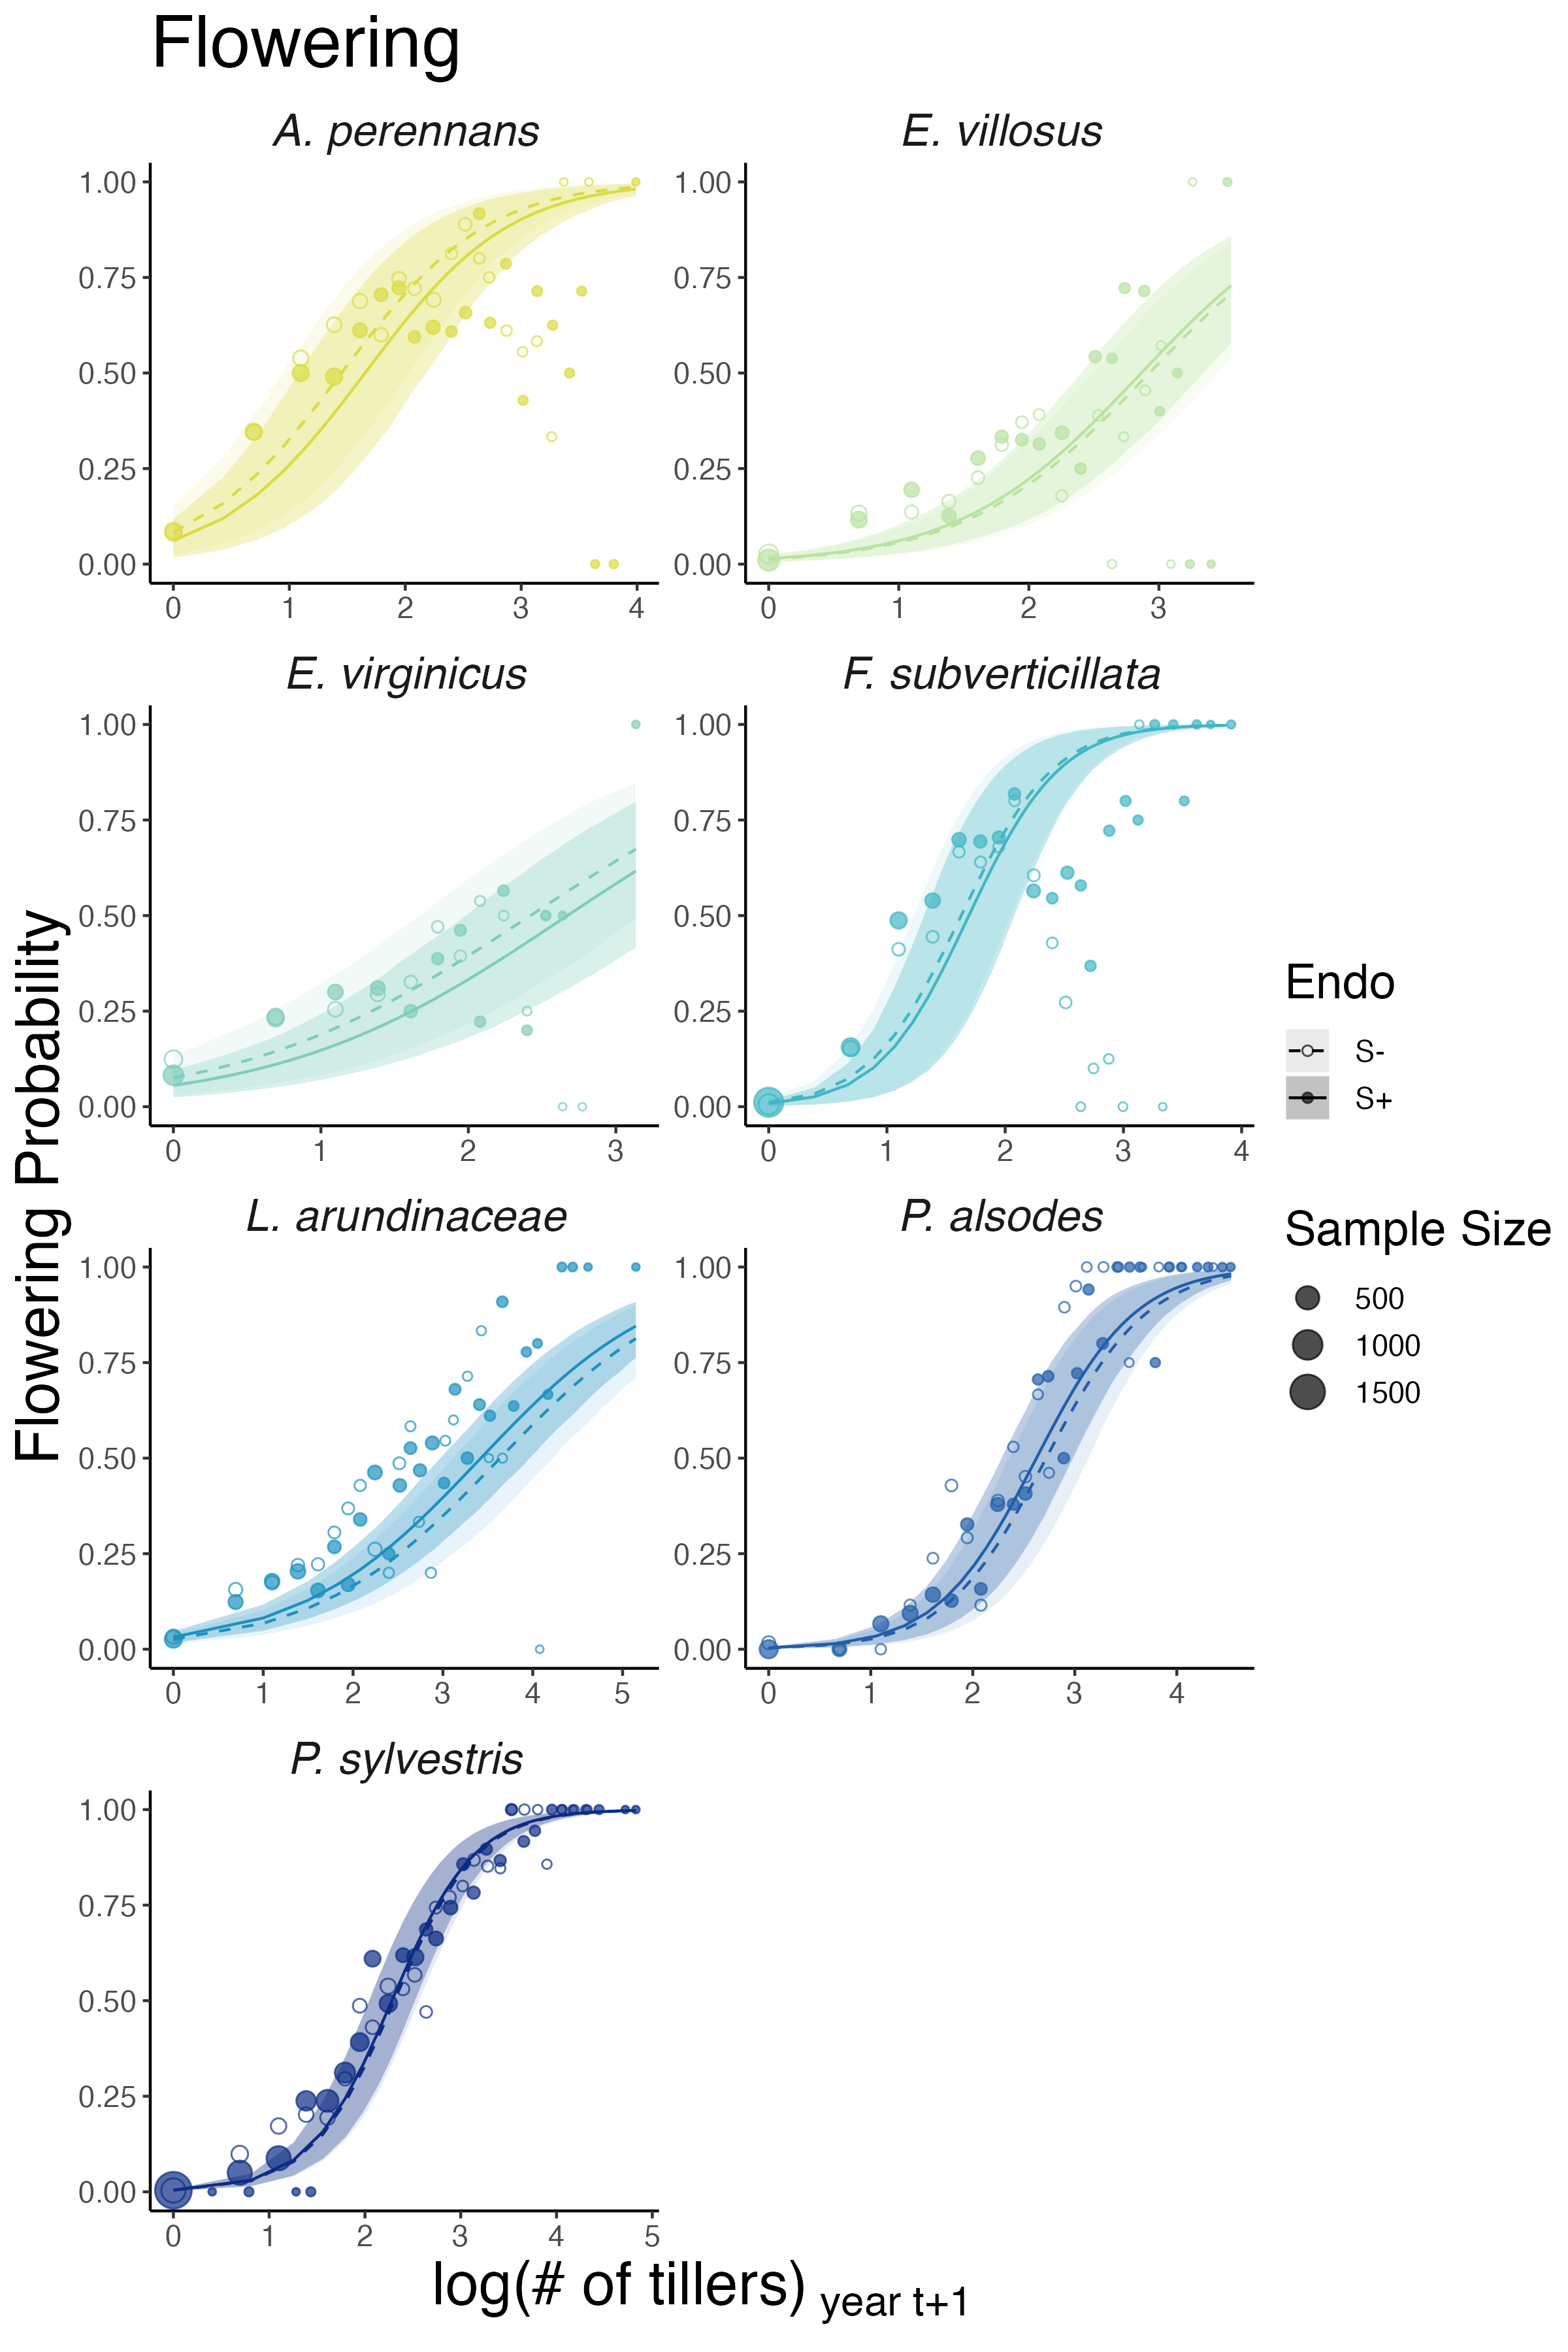
\includegraphics[width=.6\linewidth]{flw_meanplot.png}
	\caption{Effect of endophyte symbiosis on mean flowering. Fitted curves represent the size-specific mean flowering probability for original plants along with data binned by size shown as open circles with a dashed line for symbiont-free (S-) plants, while the solid line and filled circles represent symbiontic (S+) plants. 80\% credible intervals are shown with dark shading for  S+, or light shading for S-.}
\end{figure}

\begin{figure}[H]
	\centering
	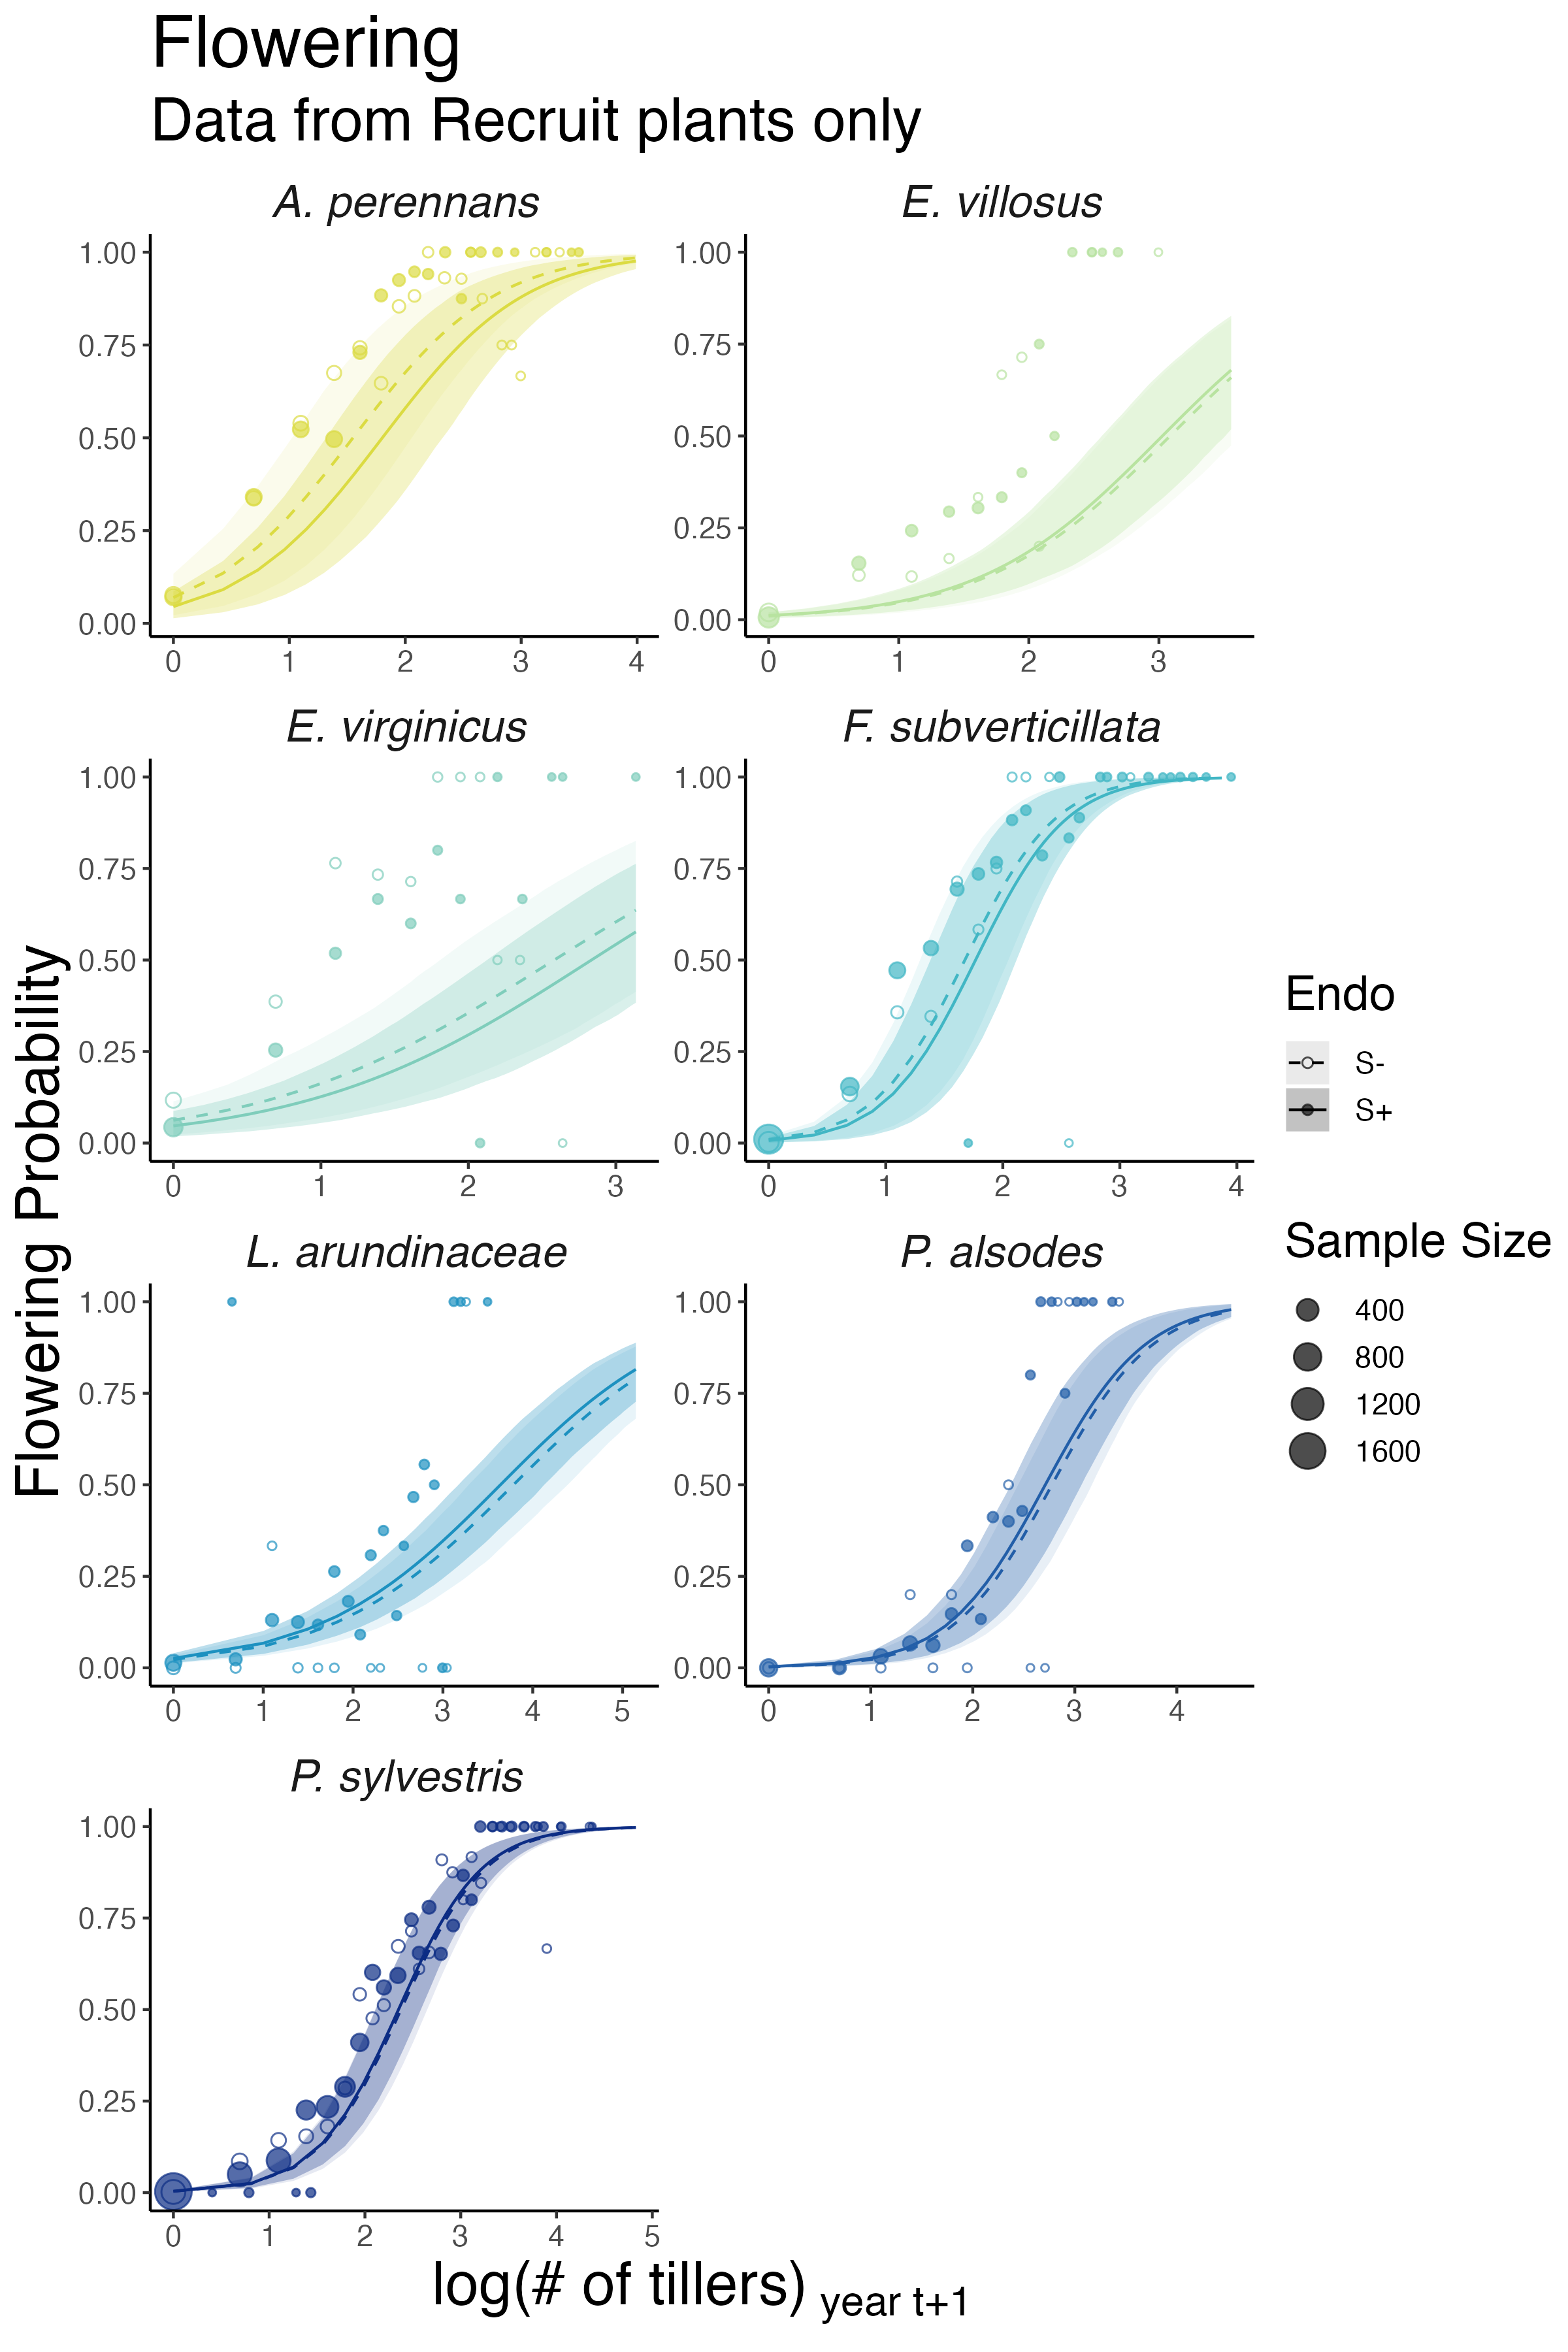
\includegraphics[width=.6\linewidth]{recruit_flw_meanplot.png}
	\caption{Effect of endophyte symbiosis on mean flowering. Fitted curves represent the size-specific mean flowering probability for recruited plants along with data binned by size shown as open circles with a dashed line for symbiont-free (S-) plants, while the solid line and filled circles represent symbiontic (S+) plants. 80\% credible intervals are shown with dark shading for  S+, or light shading for S-.}
\end{figure}

\begin{figure}[H]
	\centering
	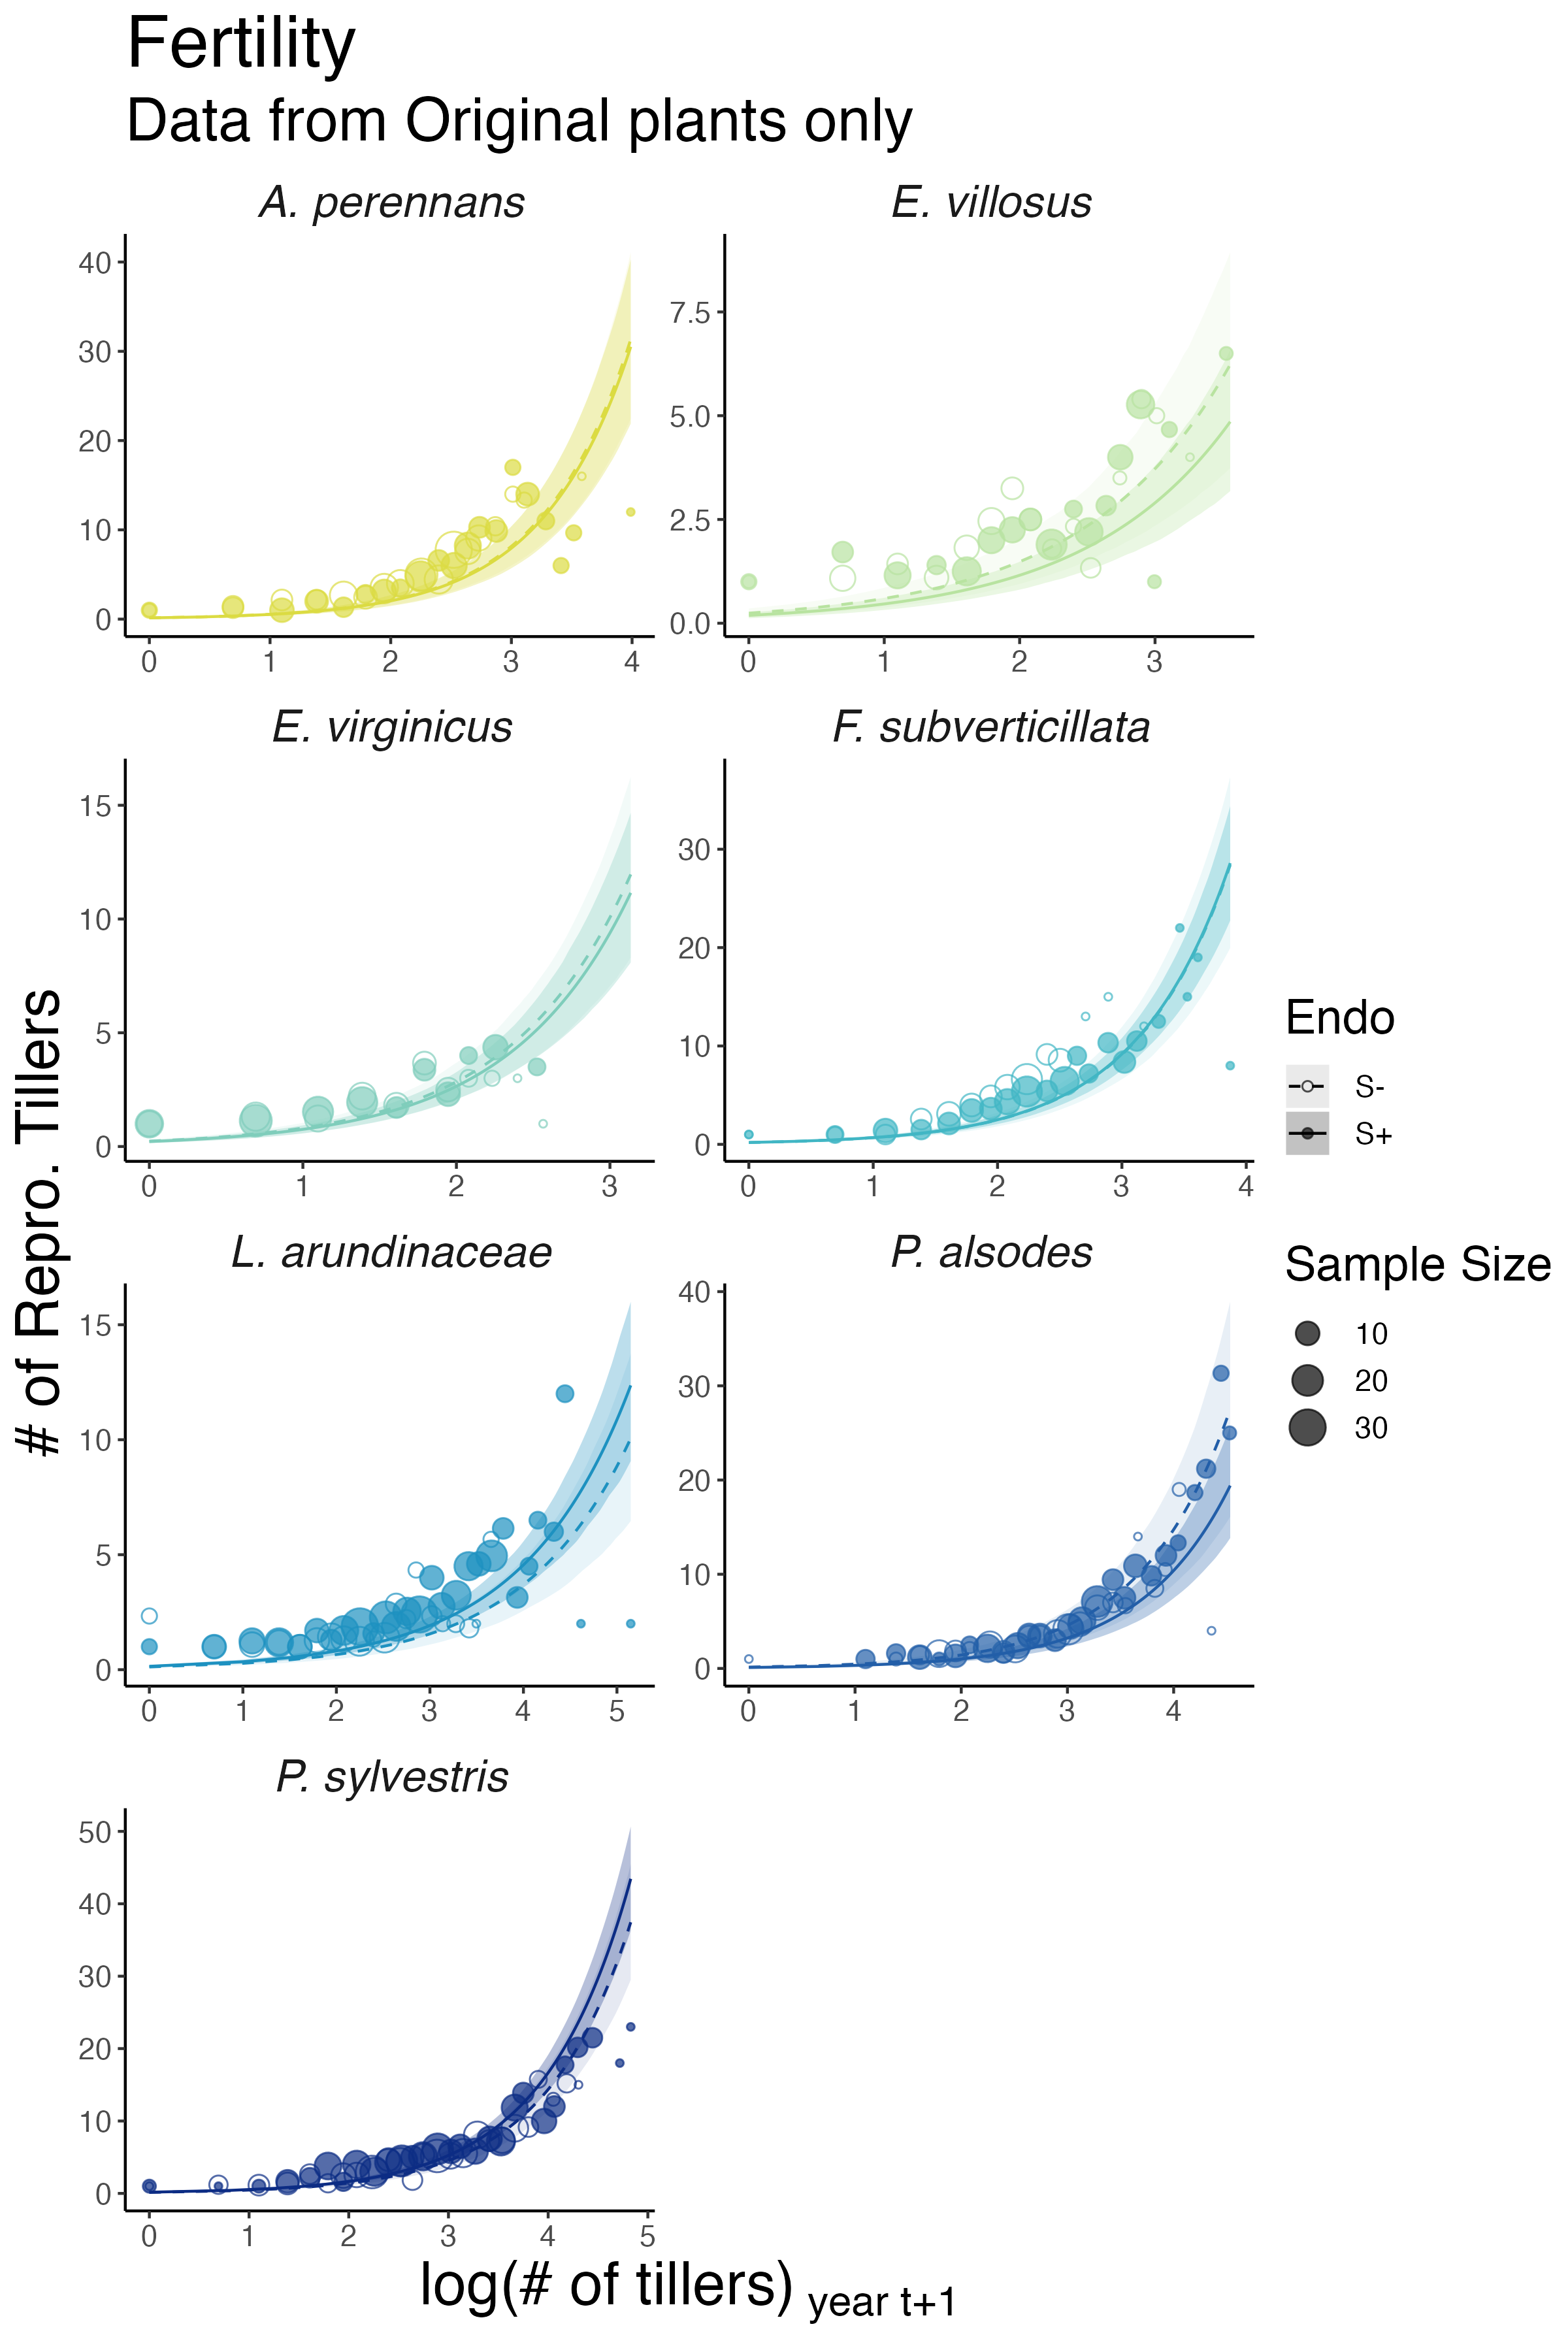
\includegraphics[width=.6\linewidth]{fert_meanplot.png}
	\caption{Effect of endophyte symbiosis on mean fertility. Fitted curves represent the size-specific mean expected number of flowering tillers for original plants along with data binned by size shown as open circles with a dashed line for symbiont-free (S-) plants, while the solid line and filled circles represent symbiontic (S+) plants. 80\% credible intervals are shown with dark shading for  S+, or light shading for S-.}
\end{figure}


\begin{figure}[H]
	\centering
	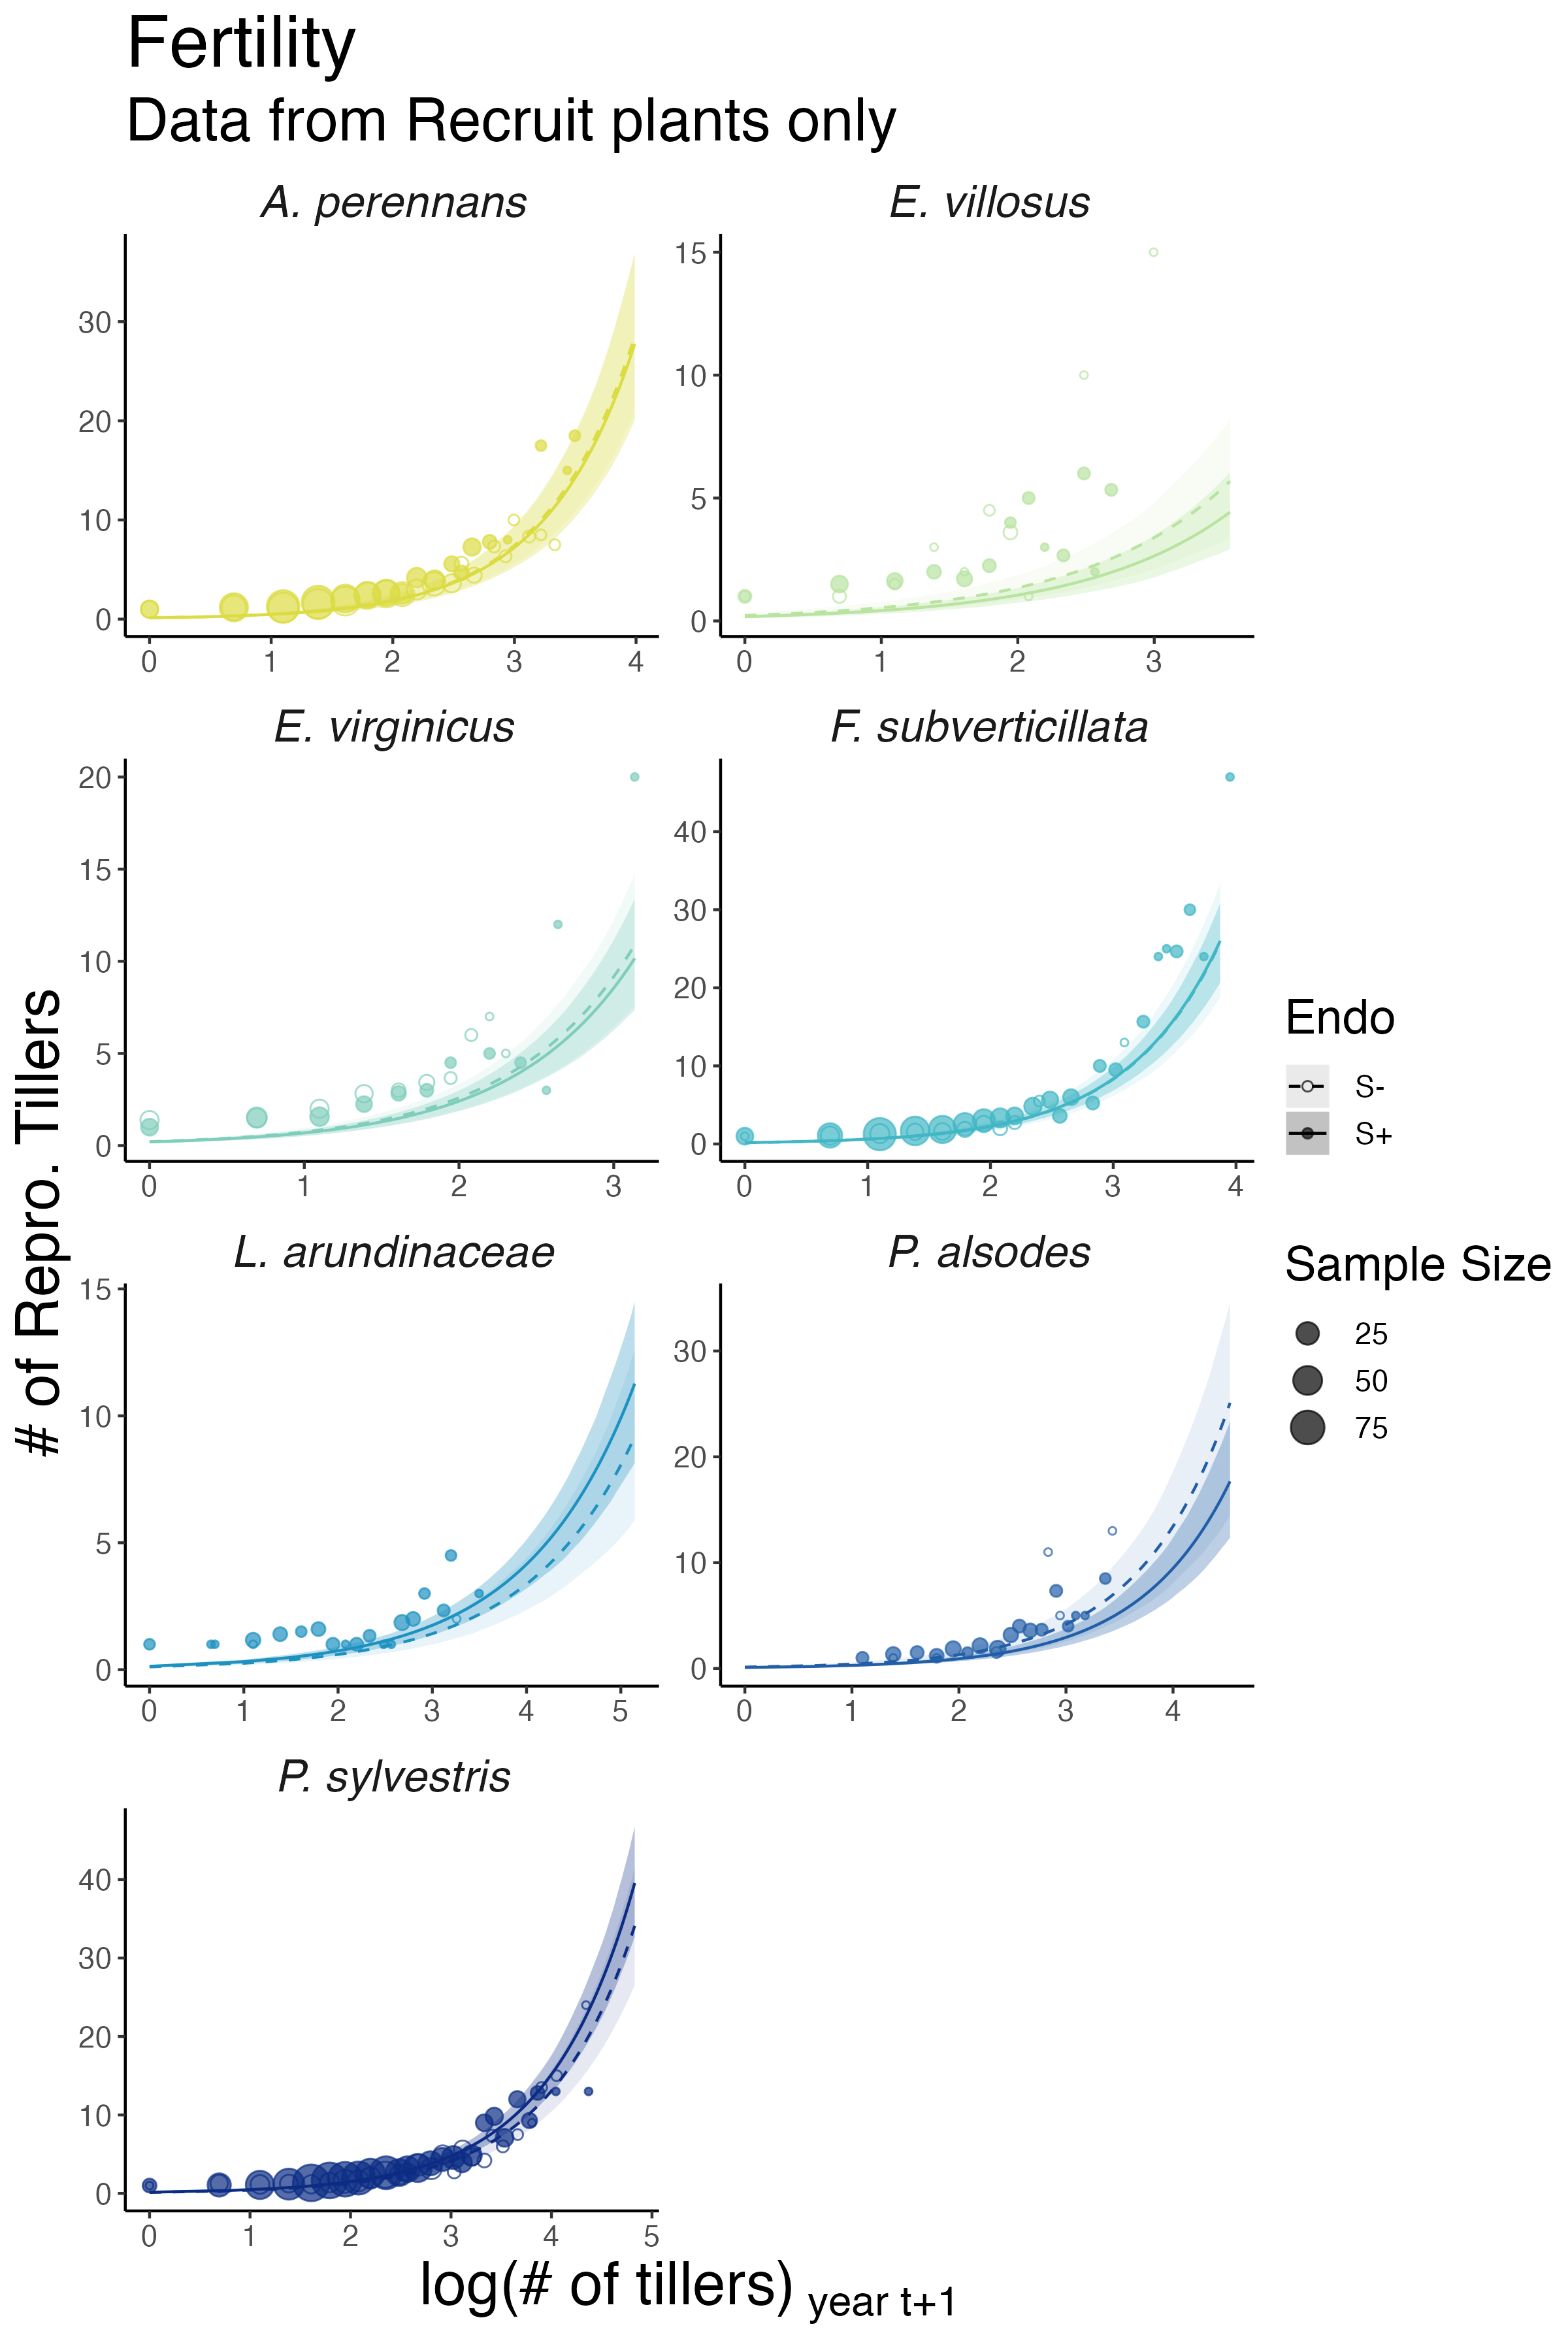
\includegraphics[width=.6\linewidth]{recruit_fert_meanplot.png}
	\caption{Effect of endophyte symbiosis on mean fertility. Fitted curves represent the size-specific mean expected number of flowering tillers for recruited plants along with data binned by size shown as open circles with a dashed line for symbiont-free (S-) plants, while the solid line and filled circles represent symbiontic (S+) plants. 80\% credible intervals are shown with dark shading for  S+, or light shading for S-.}
\end{figure}

\begin{figure}[H]
	\centering
	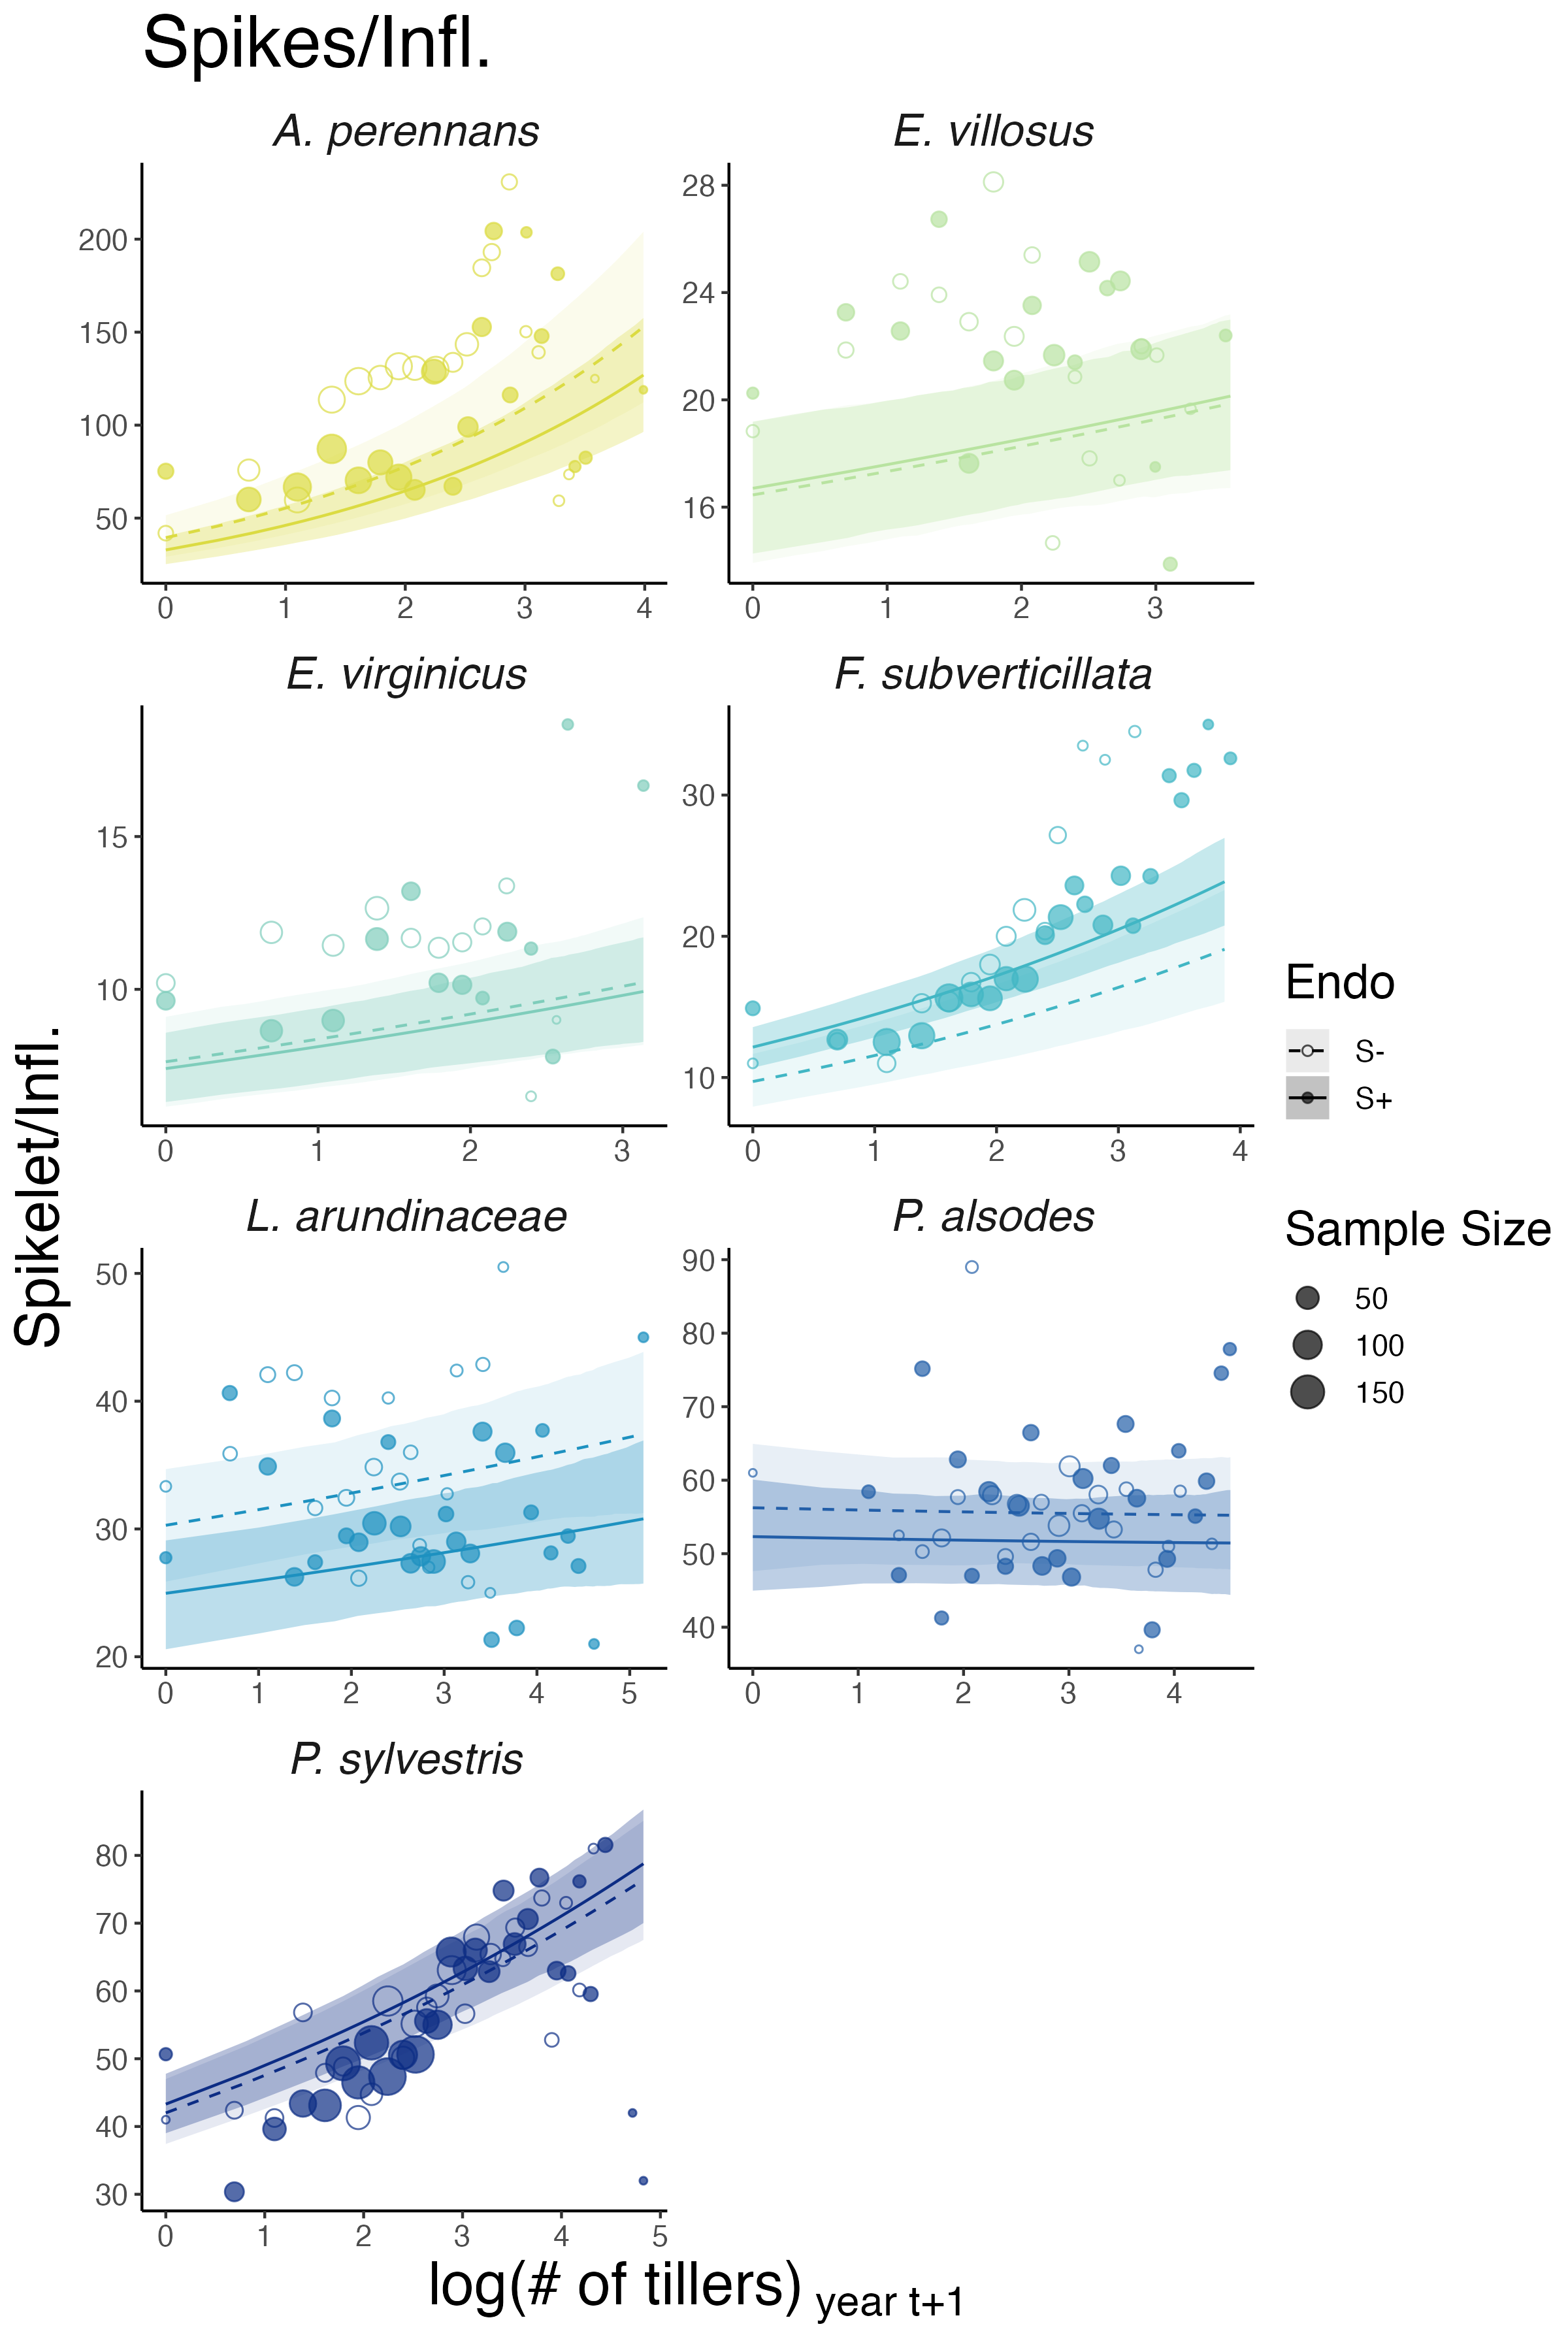
\includegraphics[width=.6\linewidth]{spike_meanplot.png}
	\caption{Effect of endophyte symbiosis on mean spikelet production. Fitted curves represent the size-specific mean expected number of spikelets per inflorescence for original plants along with data binned by size shown as open circles with a dashed line for symbiont-free (S-) plants, while the solid line and filled circles represent symbiontic (S+) plants. 80\% credible intervals are shown with dark shading for  S+, or light shading for S-.}
\end{figure}

\begin{figure}[H]
	\centering
	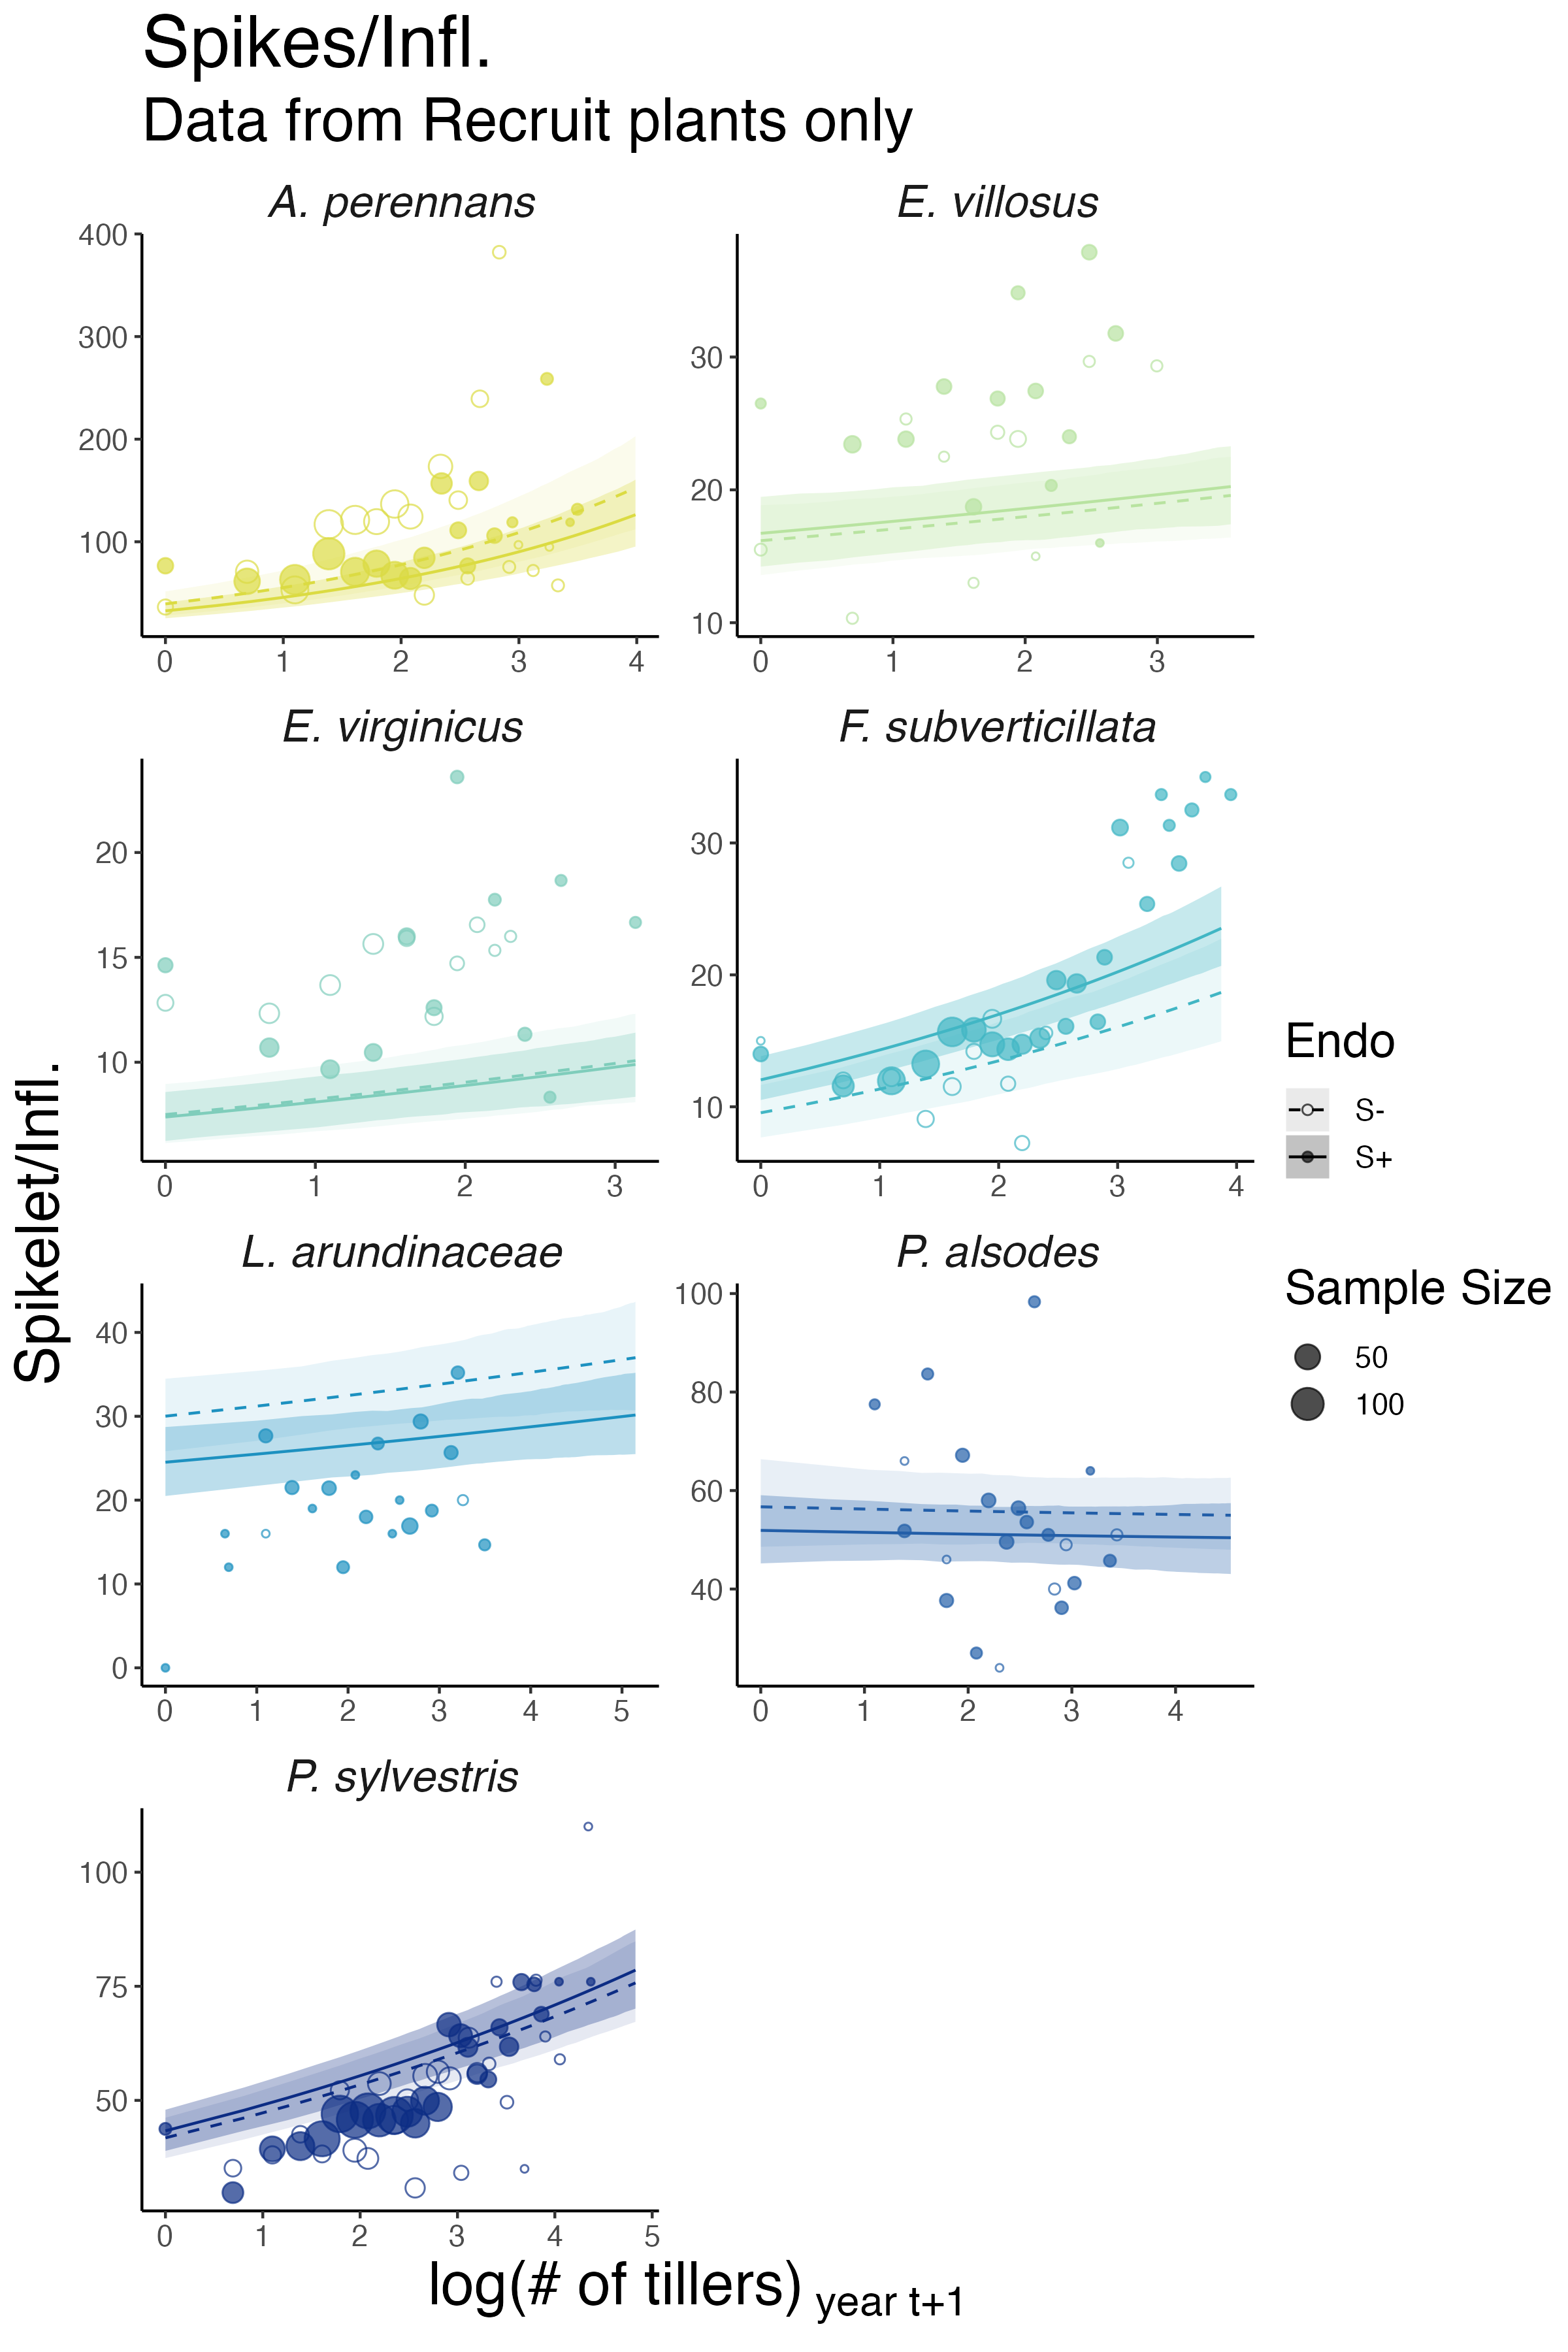
\includegraphics[width=.6\linewidth]{recruit_spike_meanplot.png}
	\caption{Effect of endophyte symbiosis on mean spikelet production. Fitted curves represent the size-specific mean expected number of spikelets per inflorescence for recruited plants along with data binned by size shown as open circles with a dashed line for symbiont-free (S-) plants, while the solid line and filled circles represent symbiontic (S+) plants. 80\% credible intervals are shown with dark shading for  S+, or light shading for S-.}
\end{figure}

\begin{figure}[H]
	\centering
	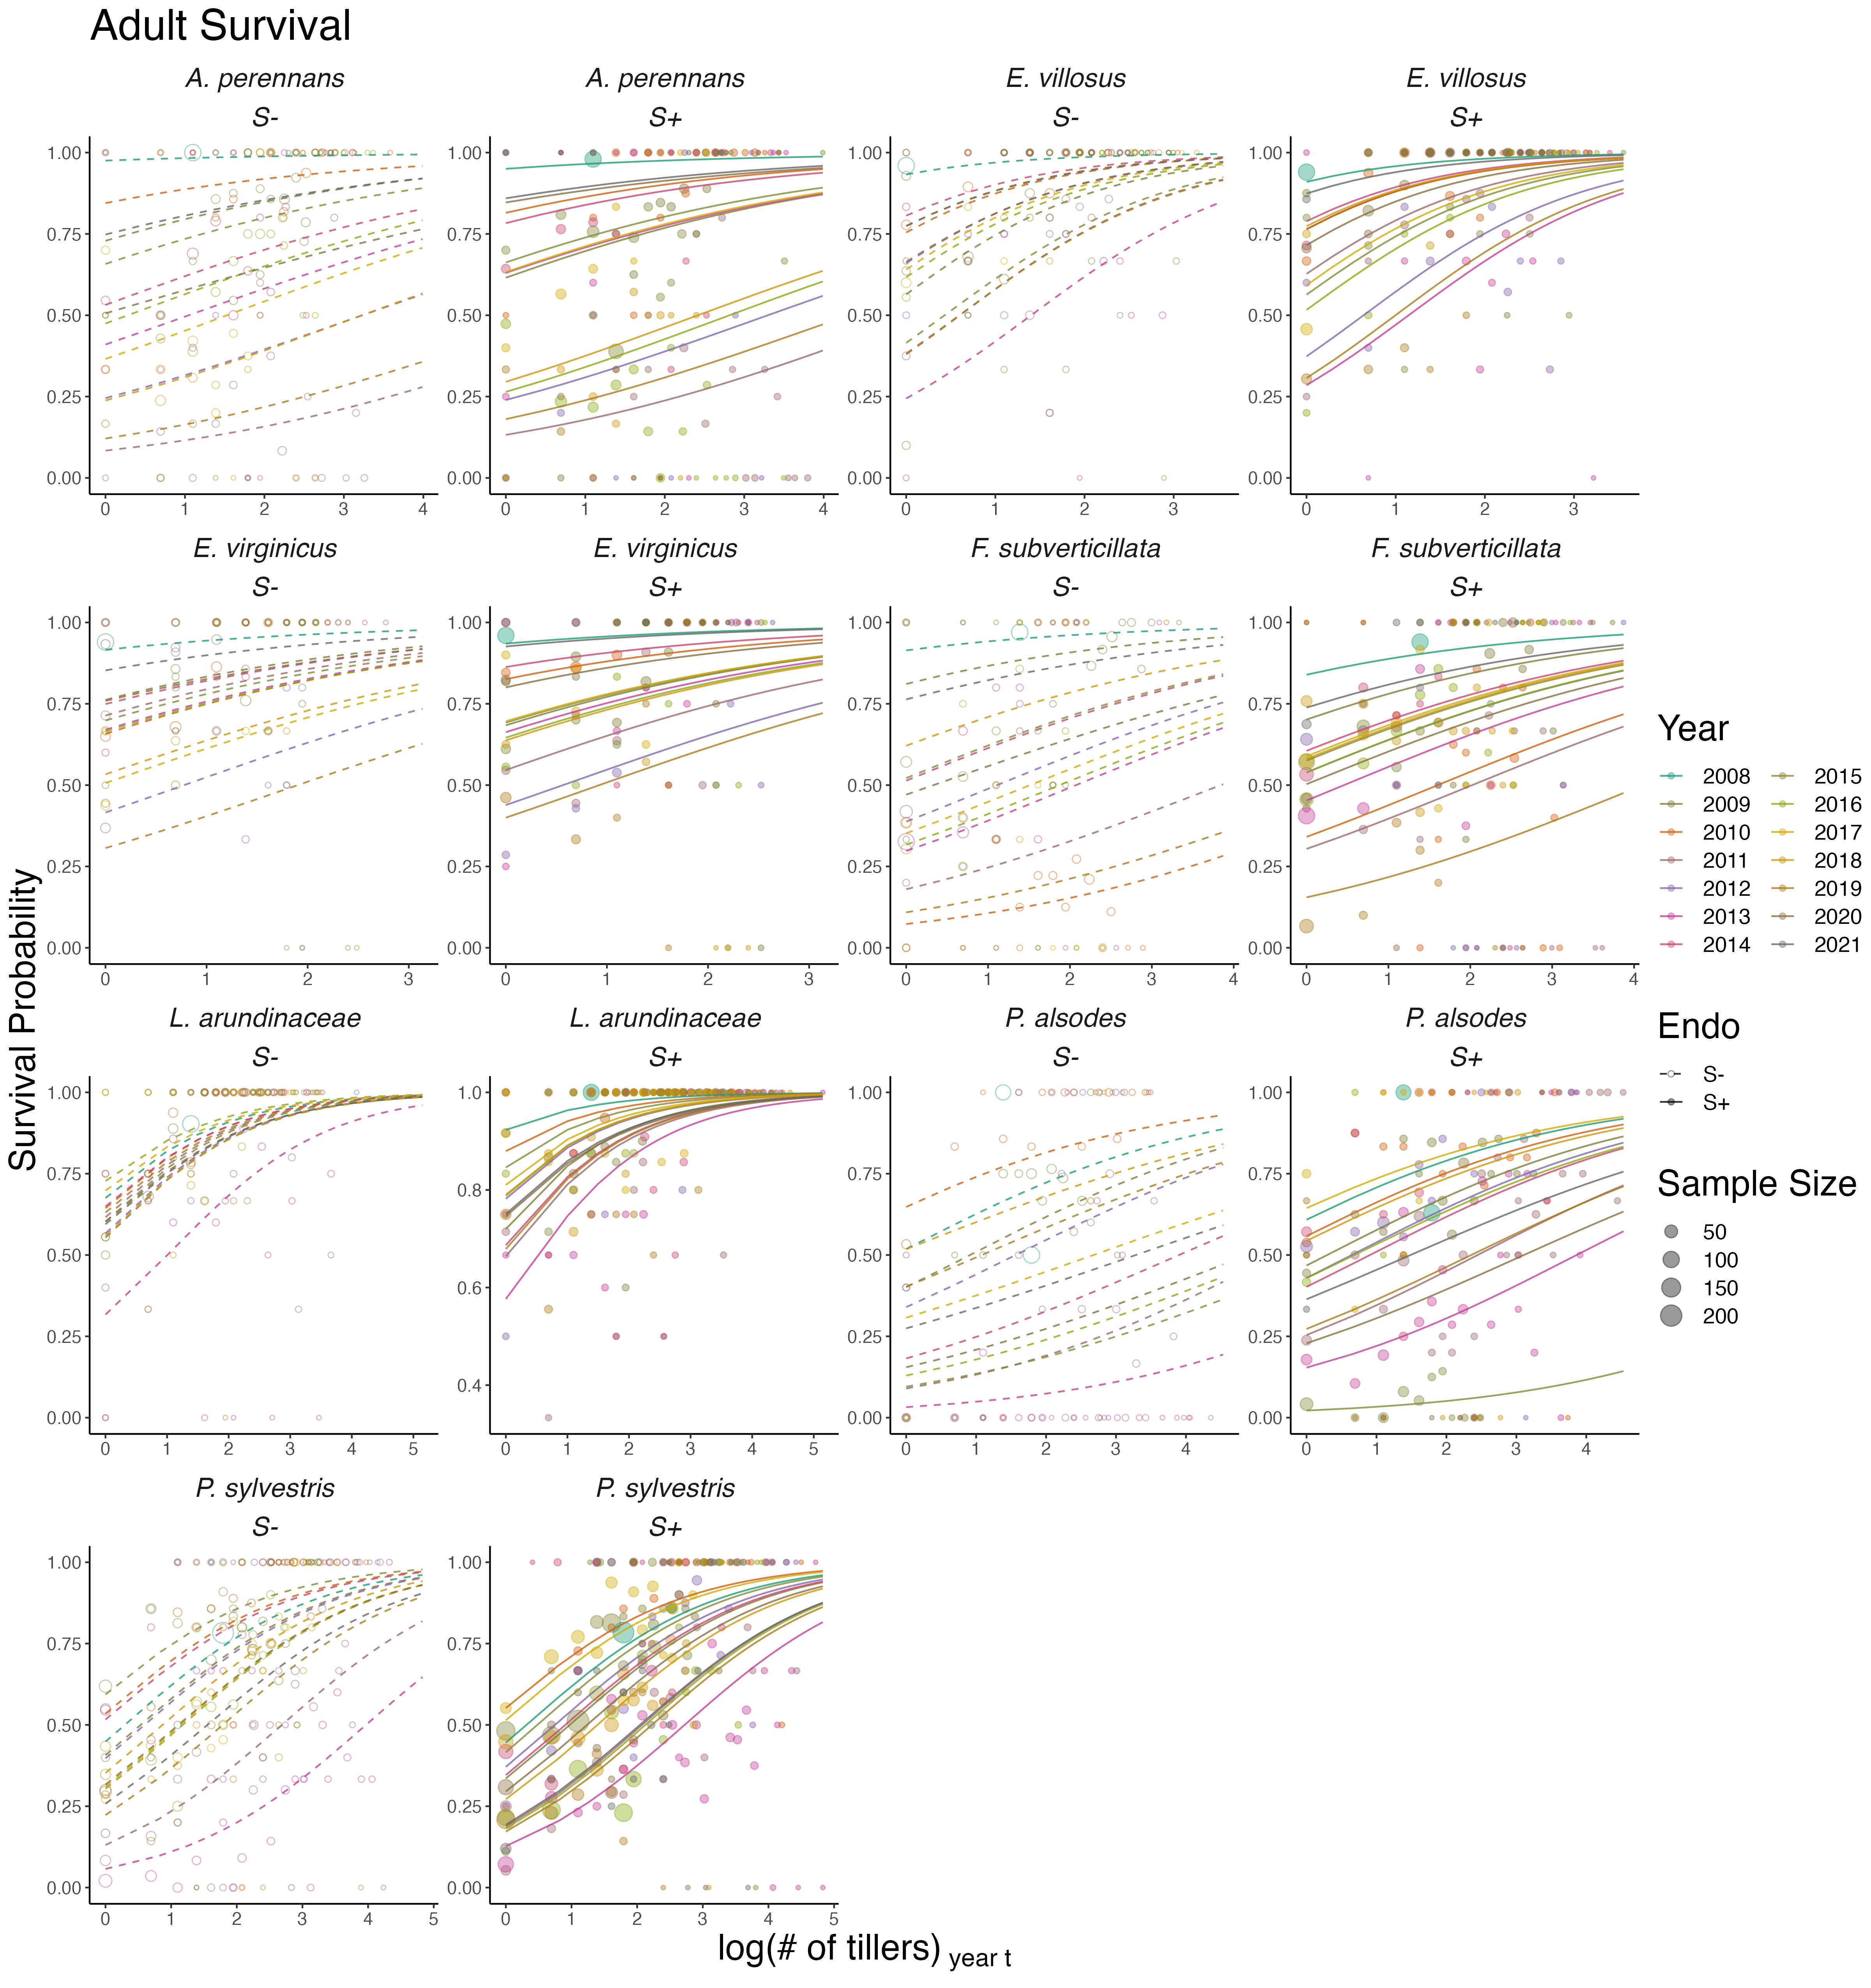
\includegraphics[width=\linewidth]{surv_yearplot.png}
	\caption{Effect of endophyte symbiosis on yearly adult survival. Fitted curves represent the size-specific annual survival probability for original plants along with data binned by size and census year shown as open circles with a dashed line for symbiont-free (S-) plants, while the solid line and filled circles represent symbiontic (S+) plants. }
\end{figure}

\begin{figure}[H]
	\centering
	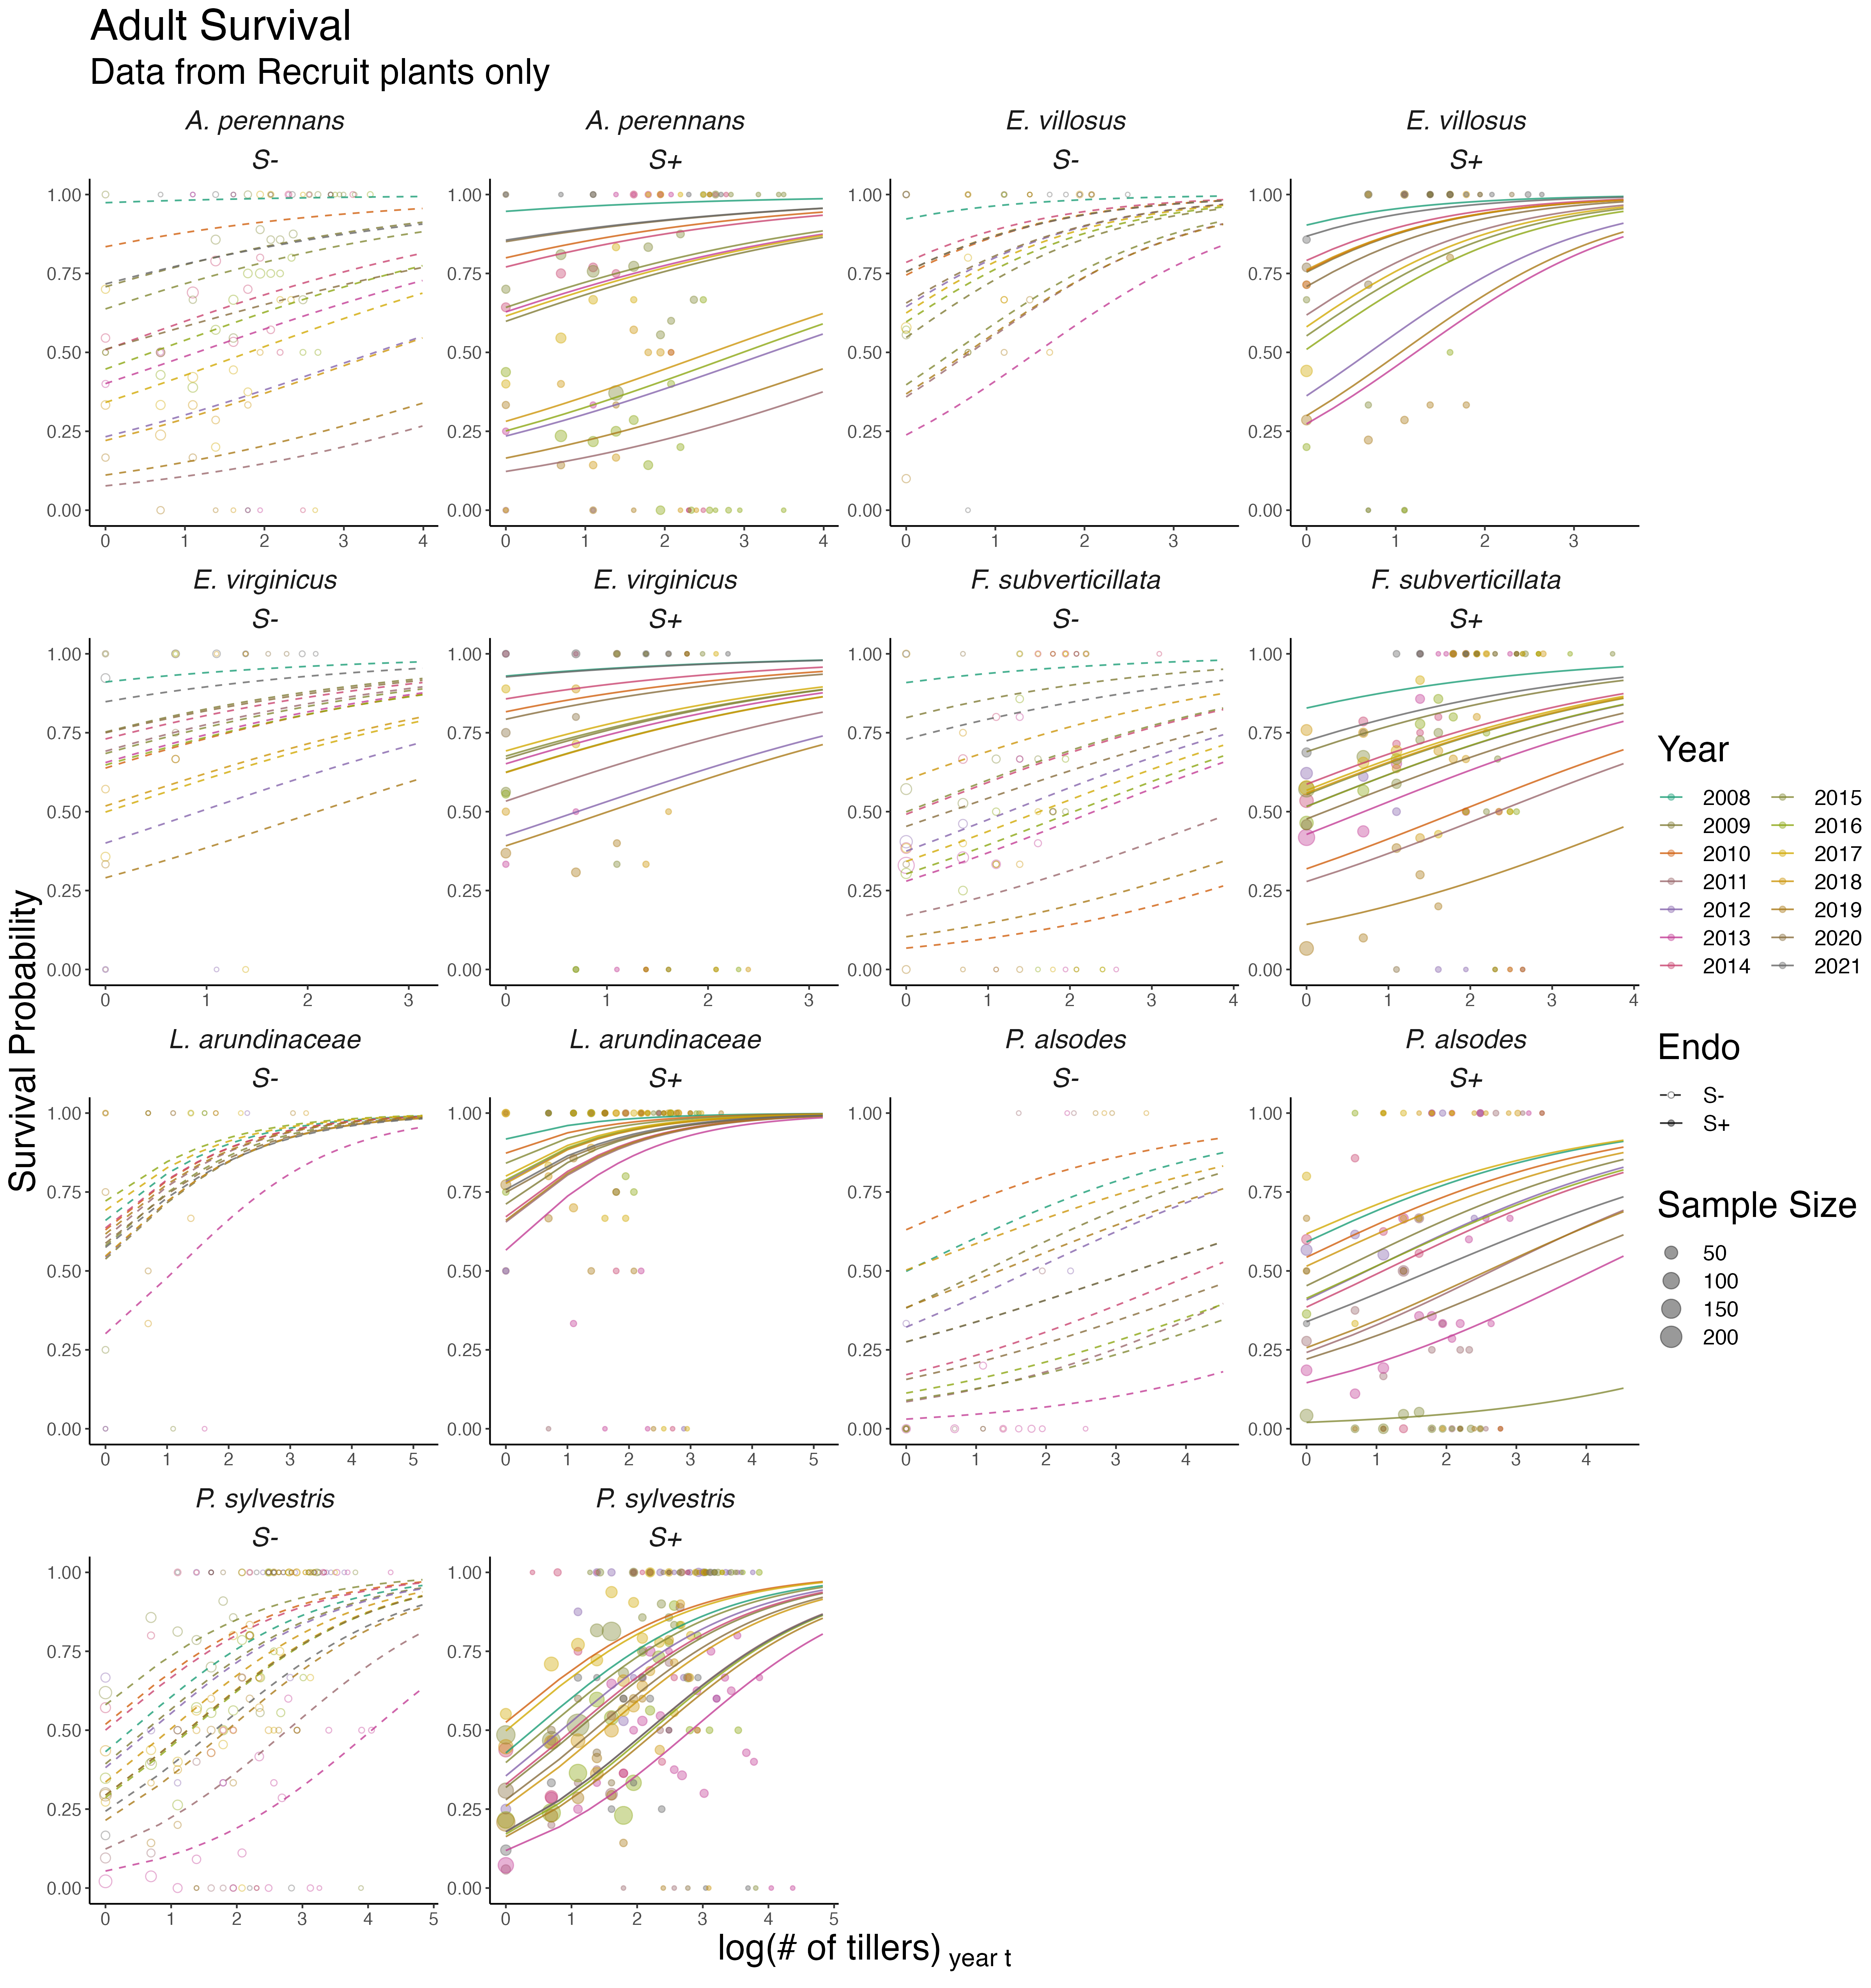
\includegraphics[width=\linewidth]{recruit_surv_yearplot.png}
	\caption{Effect of endophyte symbiosis on yearly adult survival. Fitted curves represent the size-specific annual survival probability for recruited plants along with data binned by size and census year shown as open circles with a dashed line for symbiont-free (S-) plants, while the solid line and filled circles represent symbiontic (S+) plants. }
\end{figure}

\begin{figure}[H]
	\centering
	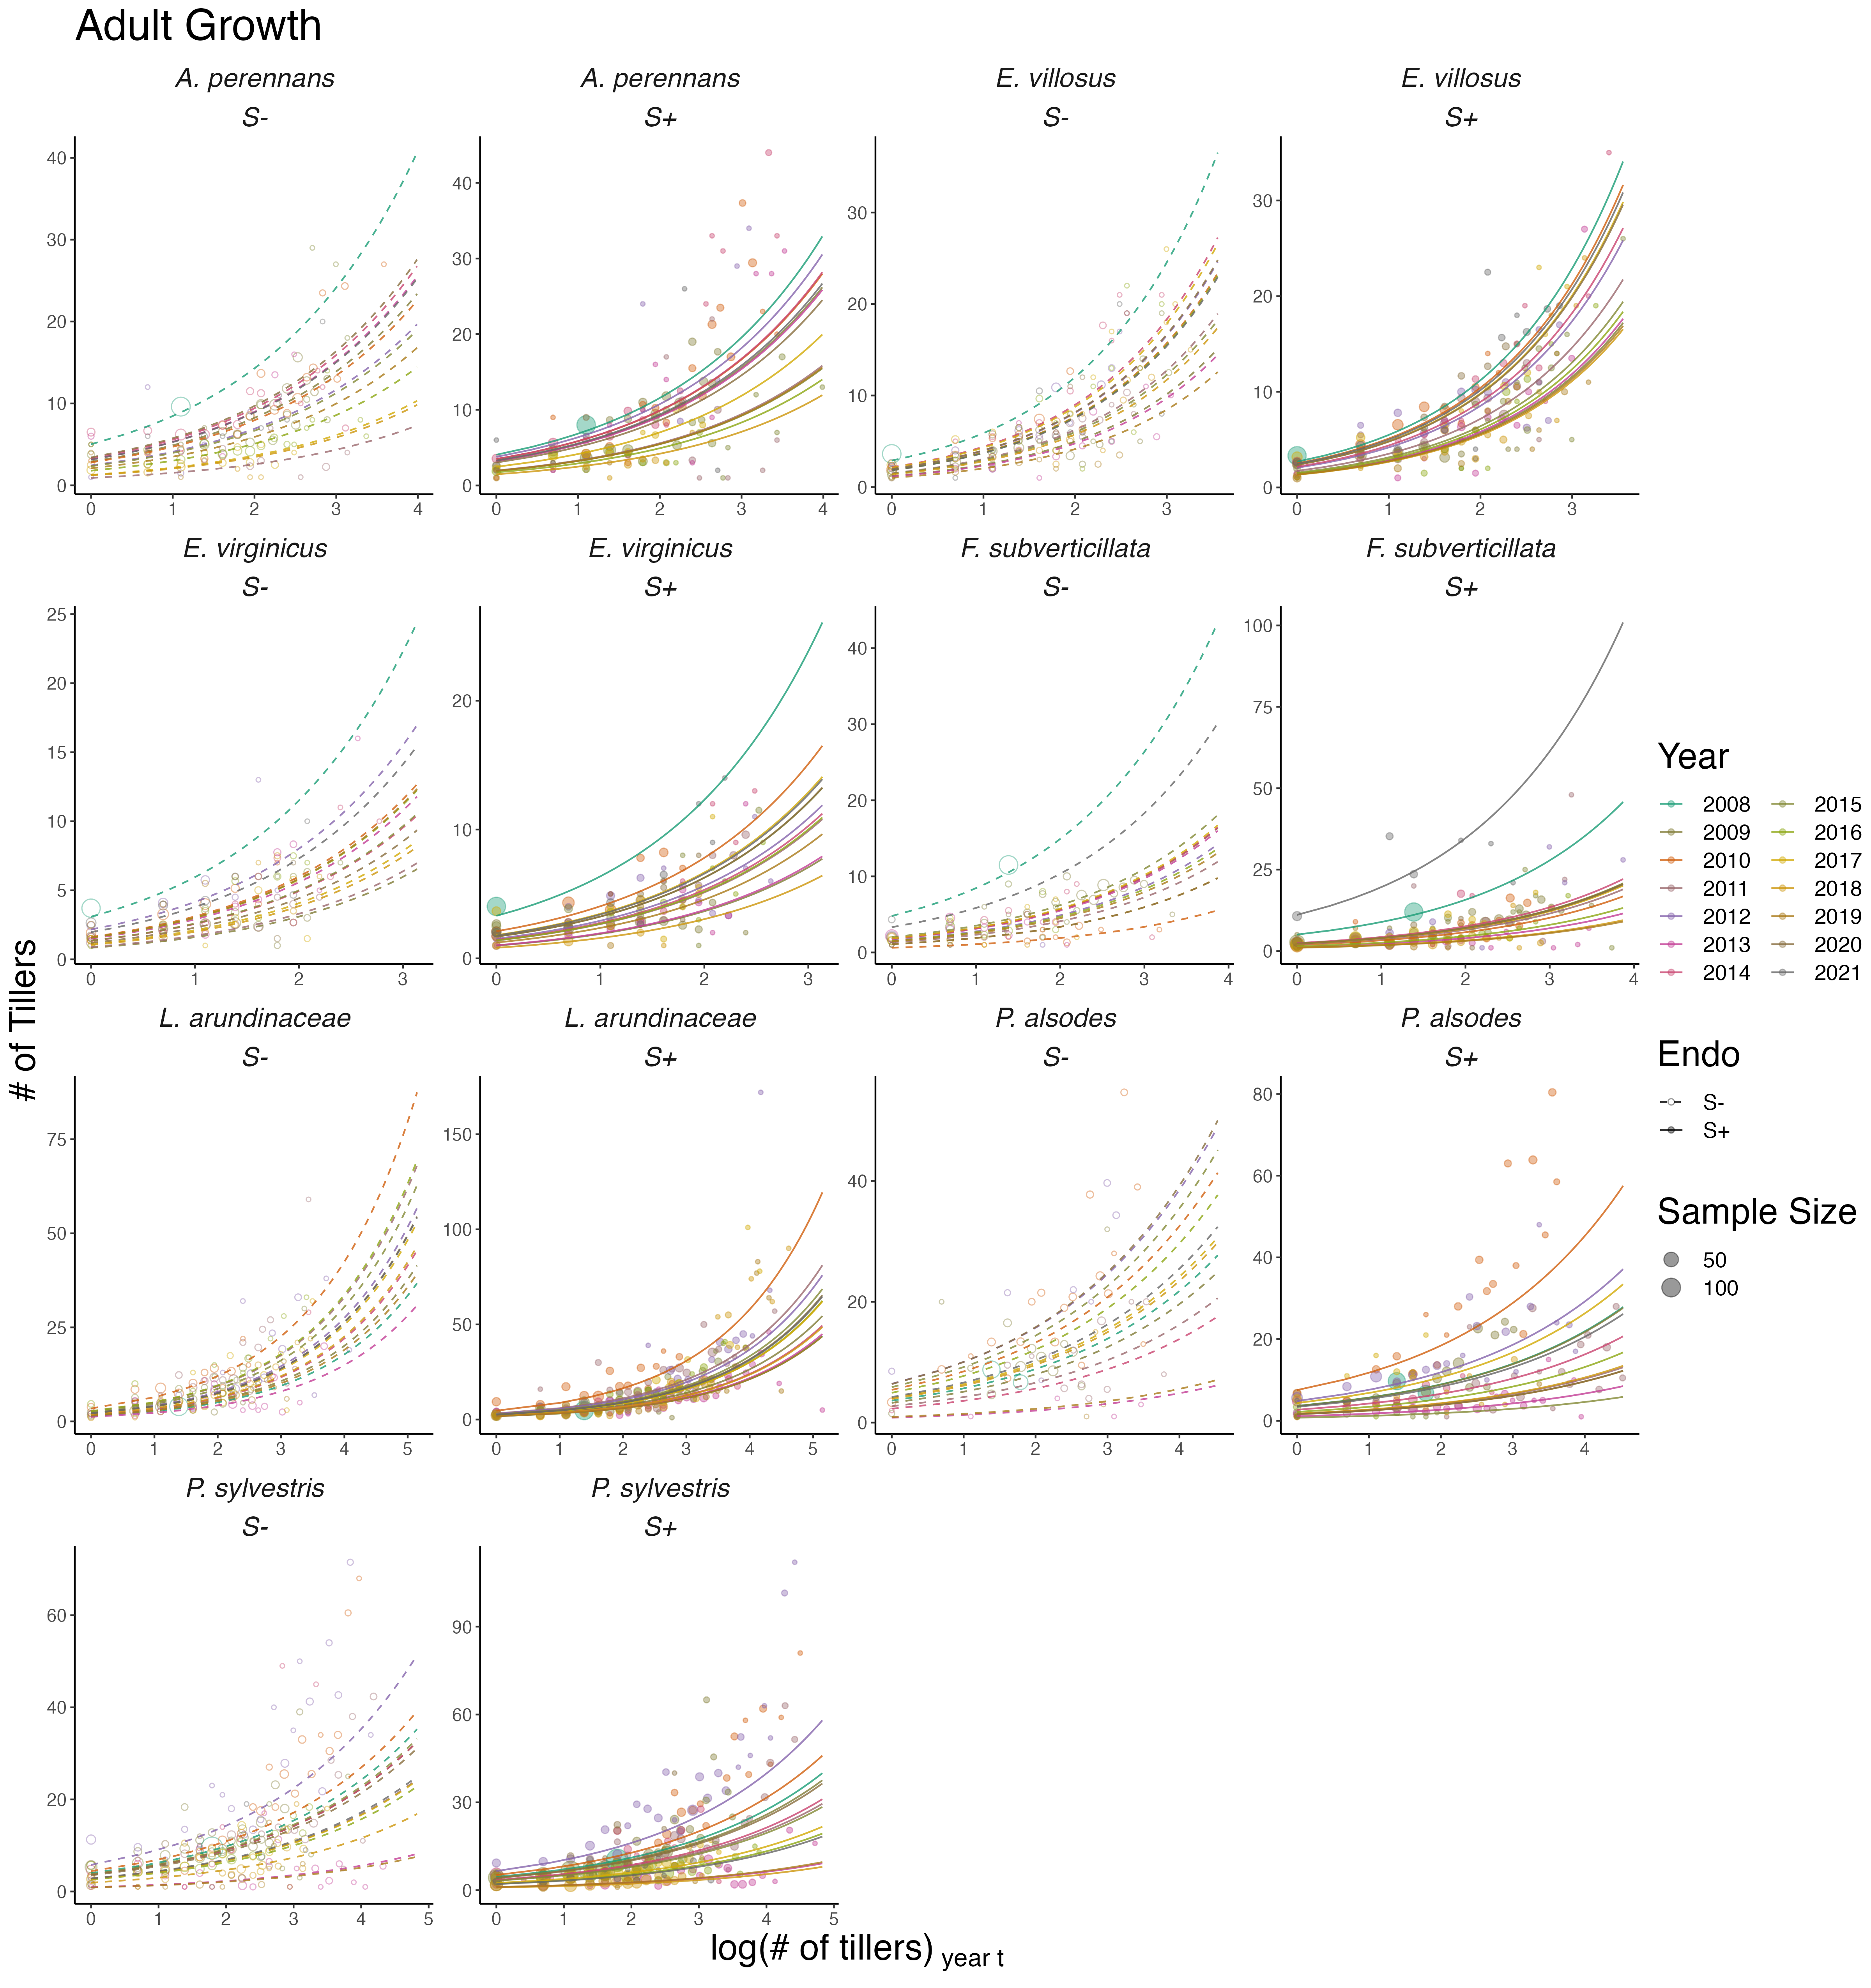
\includegraphics[width=\linewidth]{grow_yearplot.png}
	\caption{Effect of endophyte symbiosis on yearly adult growth. Fitted curves represent the size-specific annual expected plant size for original plants along with data binned by size and census year shown as open circles with a dashed line for symbiont-free (S-) plants, while the solid line and filled circles represent symbiontic (S+) plants. }
\end{figure}


\begin{figure}[H]
	\centering
	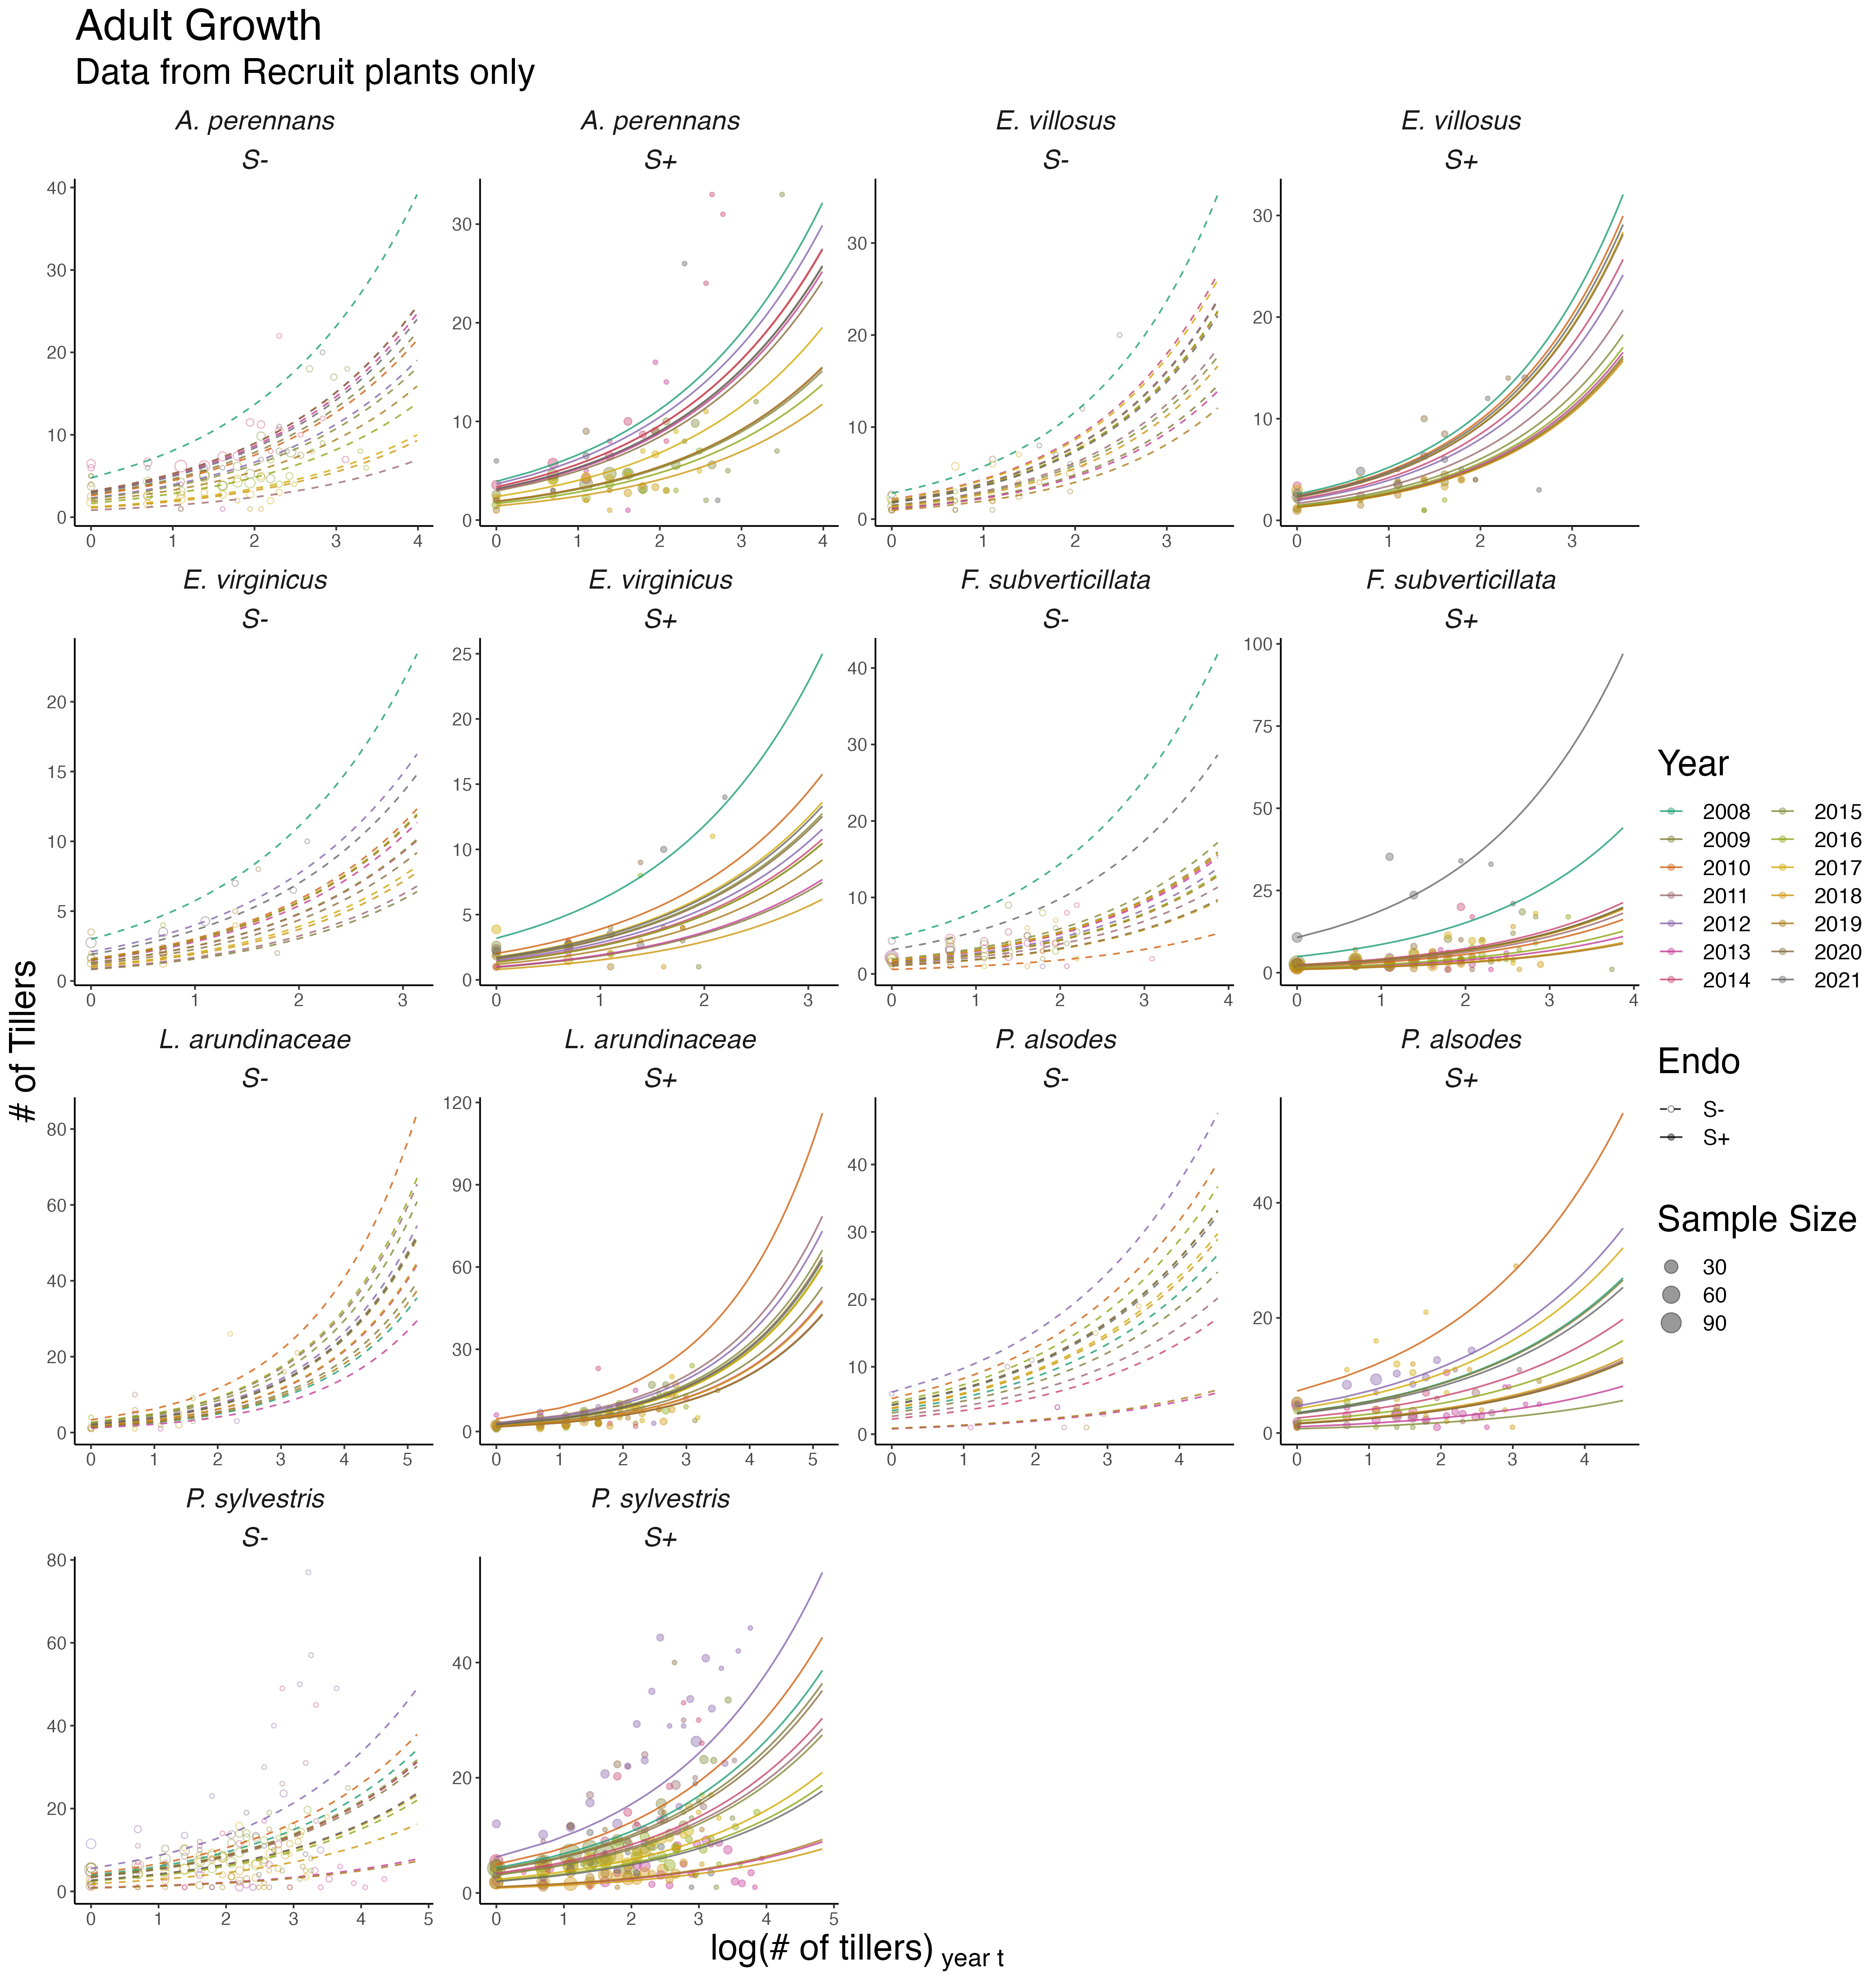
\includegraphics[width=\linewidth]{recruit_grow_yearplot.png}
	\caption{Effect of endophyte symbiosis on yearly adult growth. Fitted curves represent the size-specific annual expected plant size for recruited plants along with data binned by size and census year shown as open circles with a dashed line for symbiont-free (S-) plants, while the solid line and filled circles represent symbiontic (S+) plants. }
\end{figure}

\begin{figure}[H]
	\centering
	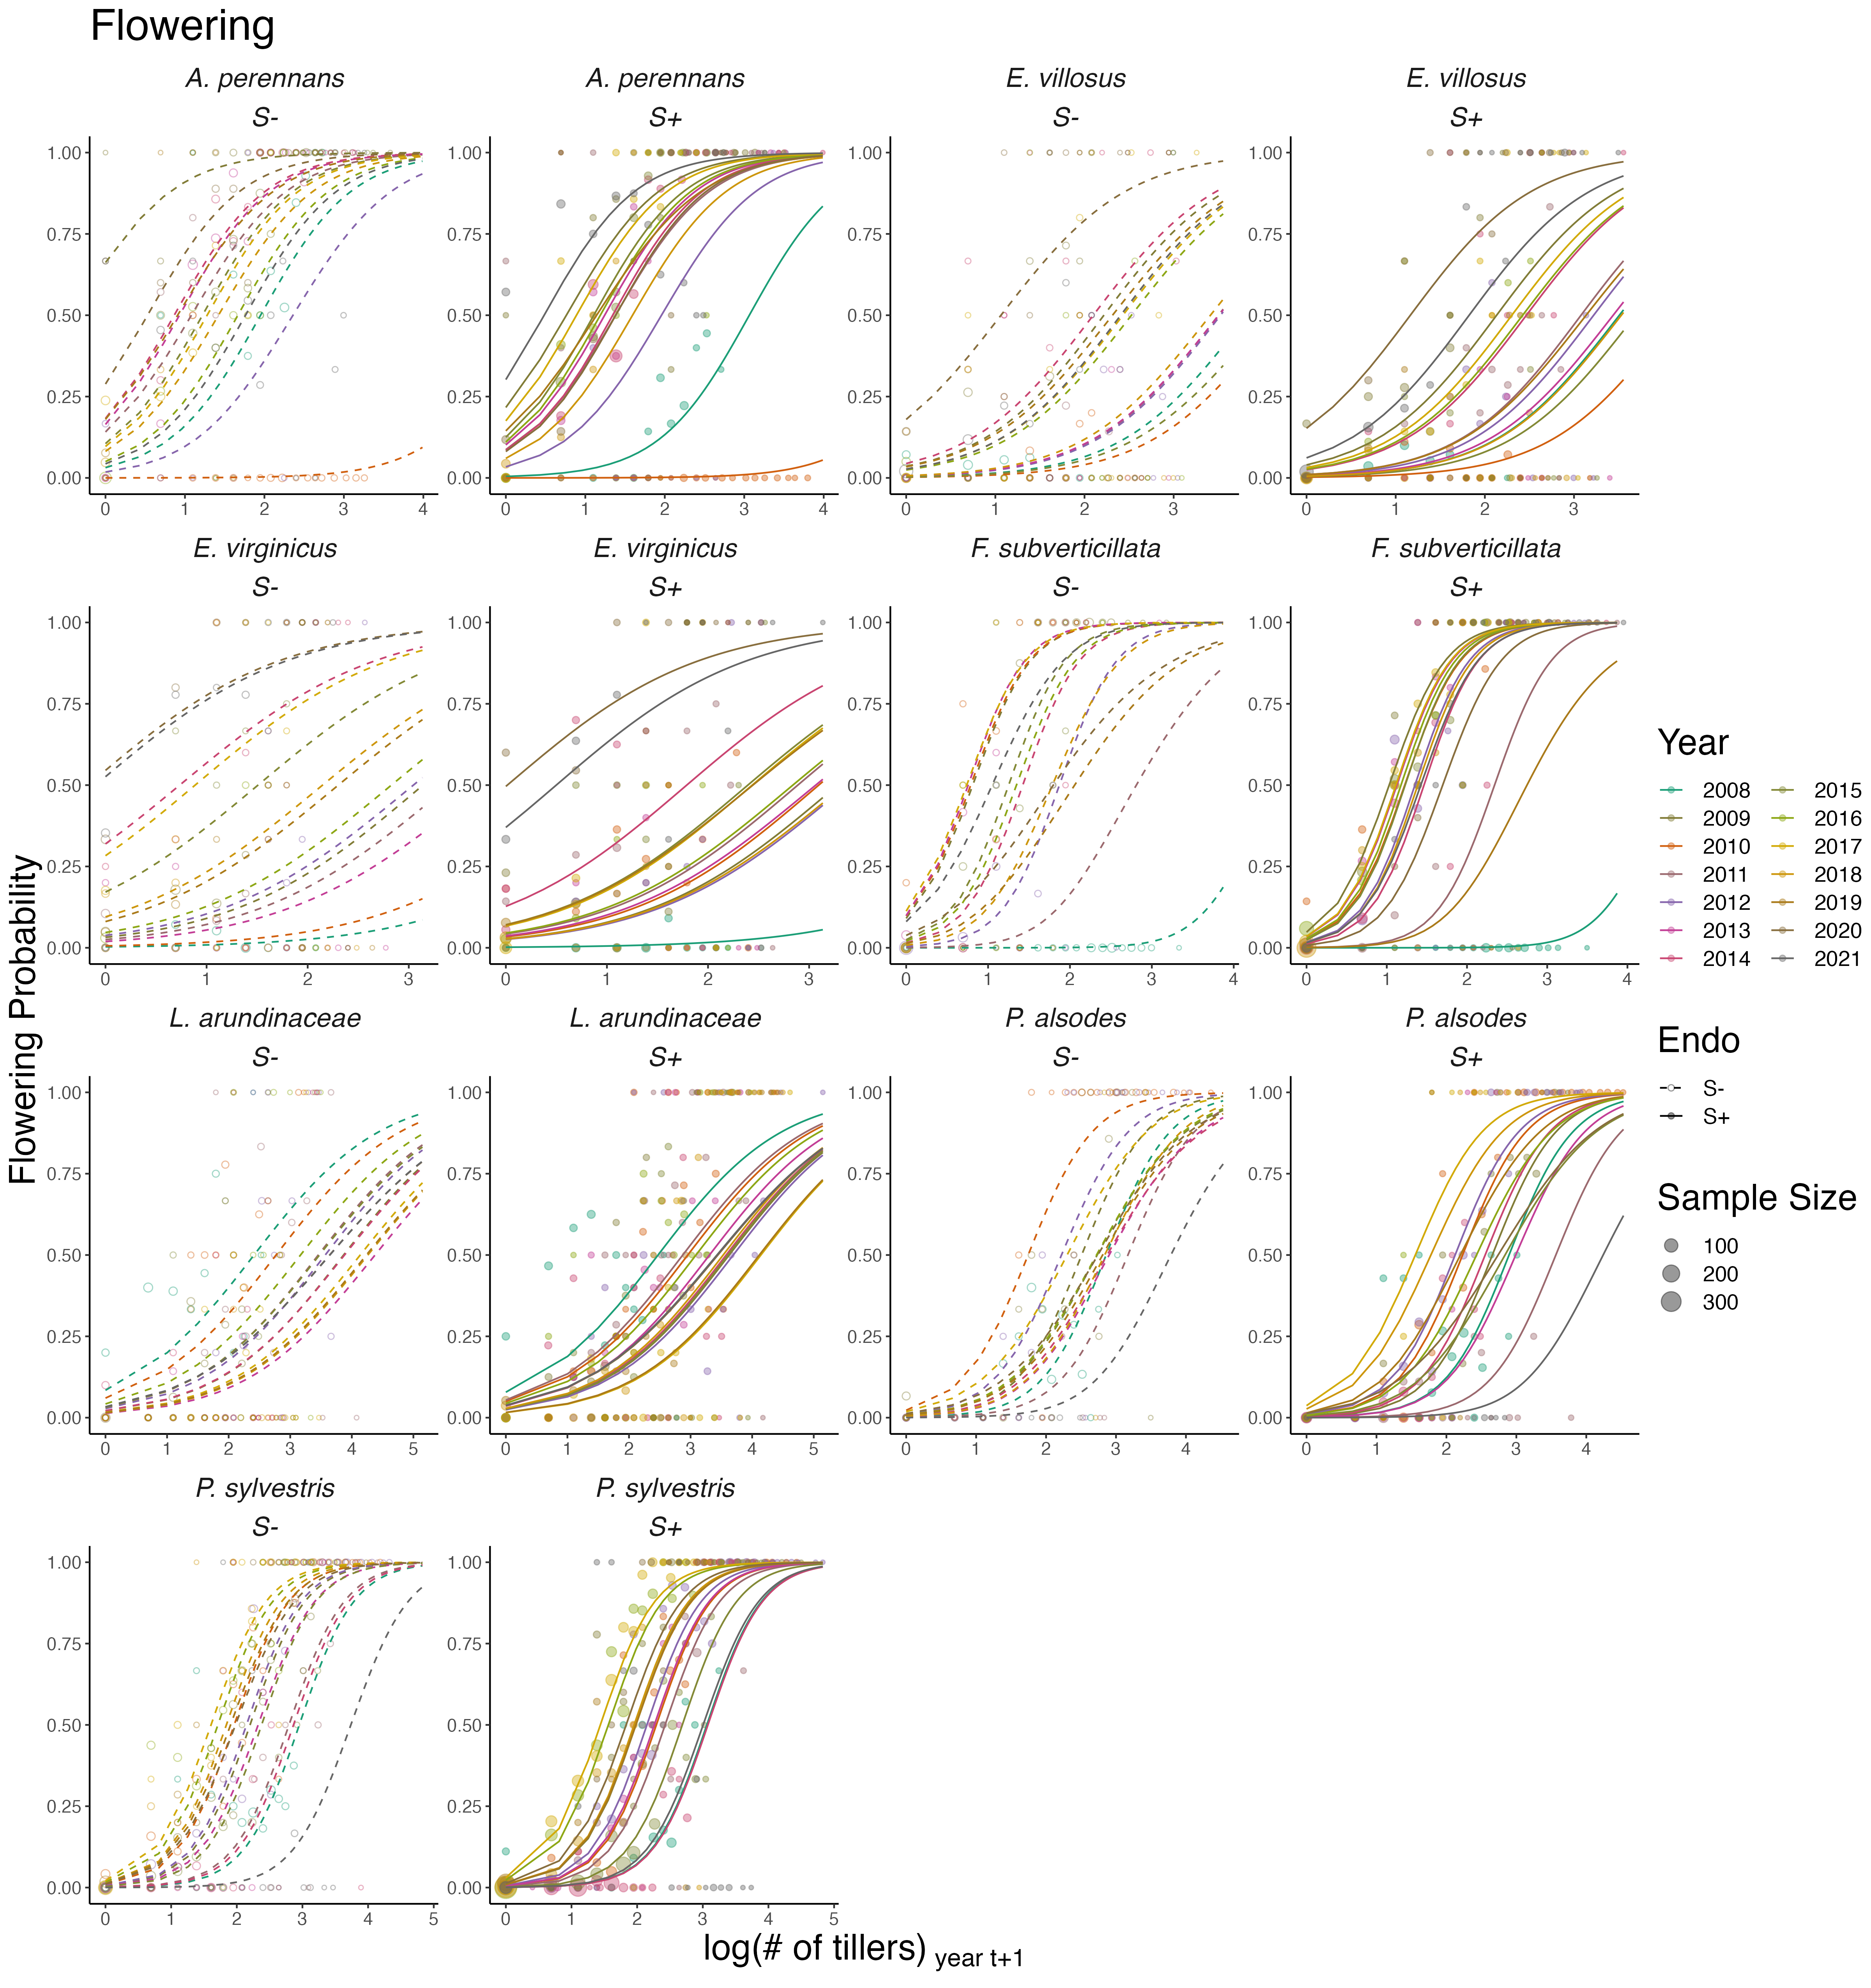
\includegraphics[width=\linewidth]{flw_yearplot.png}
	\caption{Effect of endophyte symbiosis on yearly flowering. Fitted curves represent the size-specific annual flowering probability for original plants along with data binned by size and census year shown as open circles with a dashed line for symbiont-free (S-) plants, while the solid line and filled circles represent symbiontic (S+) plants.}
\end{figure}

\begin{figure}[H]
	\centering
	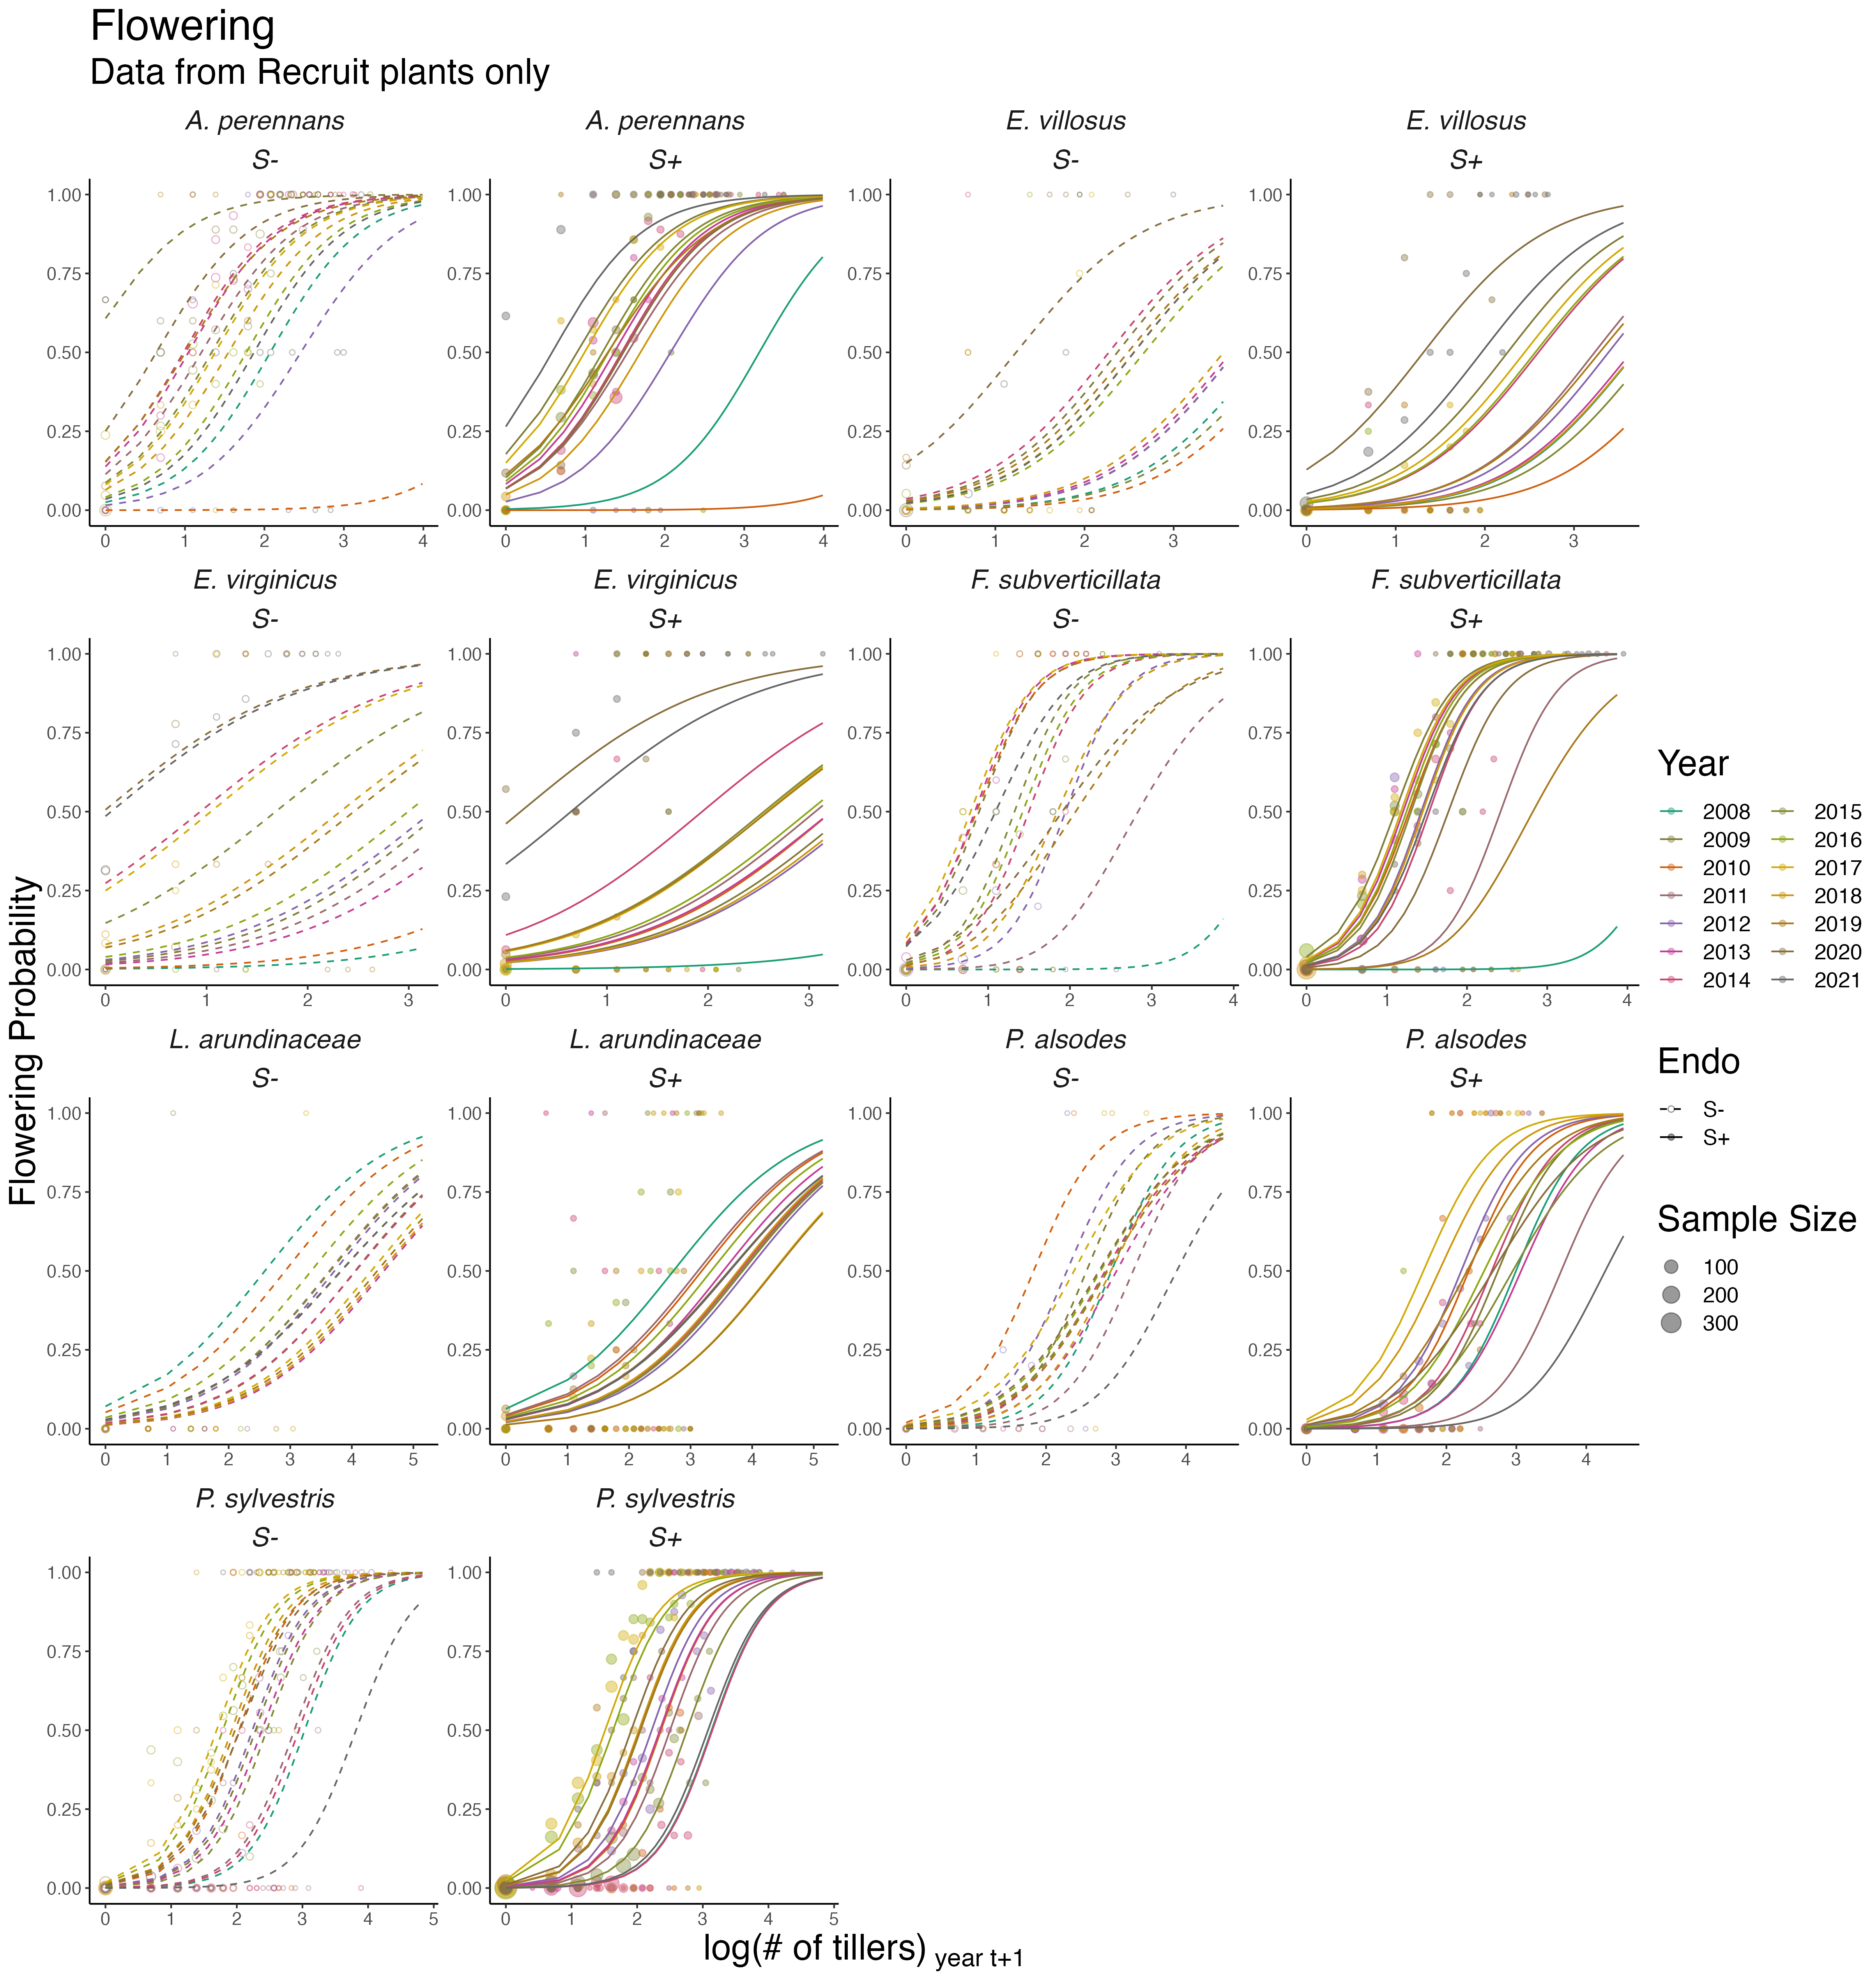
\includegraphics[width=\linewidth]{recruit_flw_yearplot.png}
	\caption{Effect of endophyte symbiosis on yearly flowering. Fitted curves represent the size-specific annual flowering probability for recruited plants along with data binned by size and census year shown as open circles with a dashed line for symbiont-free (S-) plants, while the solid line and filled circles represent symbiontic (S+) plants.}
\end{figure}


\begin{figure}[H]
	\centering
	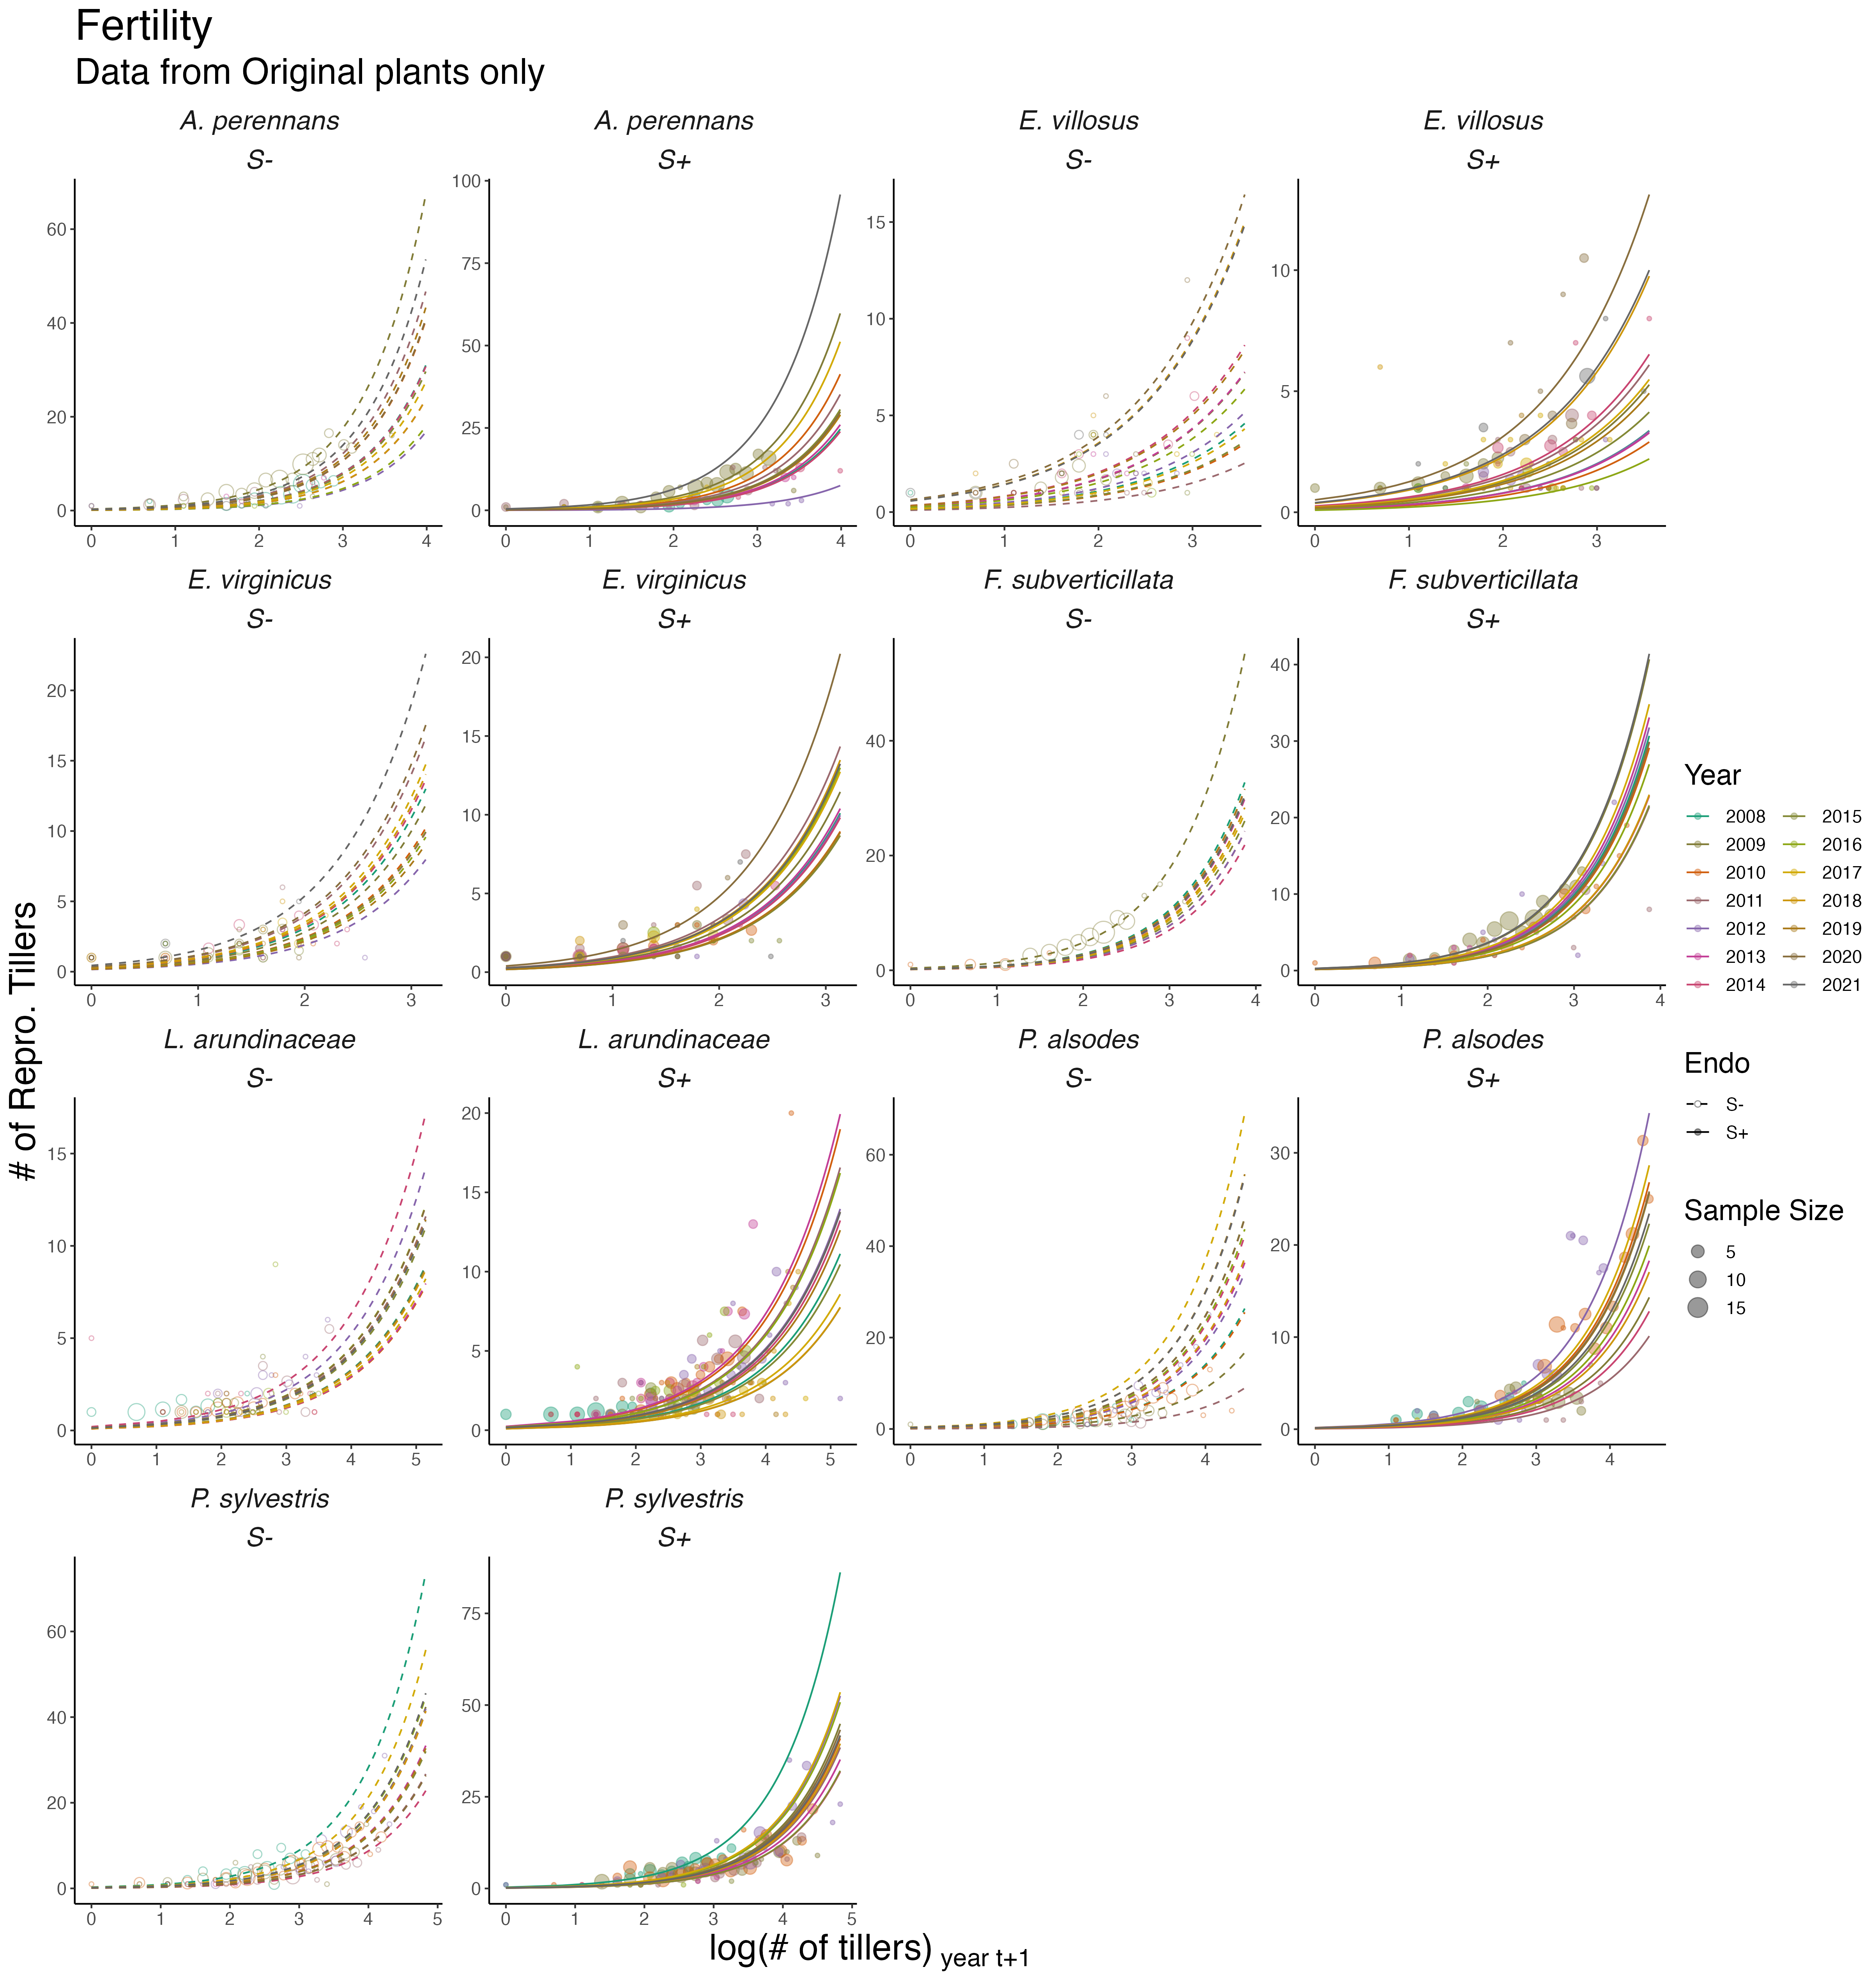
\includegraphics[width=\linewidth]{fert_yearplot.png}
	\caption{Effect of endophyte symbiosis on yearly fertility. Fitted curves represent the size-specific annual expected number of flowering tillers for original plants along with data binned by size and census year shown as open circles with a dashed line for symbiont-free (S-) plants, while the solid line and filled circles represent symbiontic (S+) plants.}
\end{figure}

\begin{figure}[H]
	\centering
	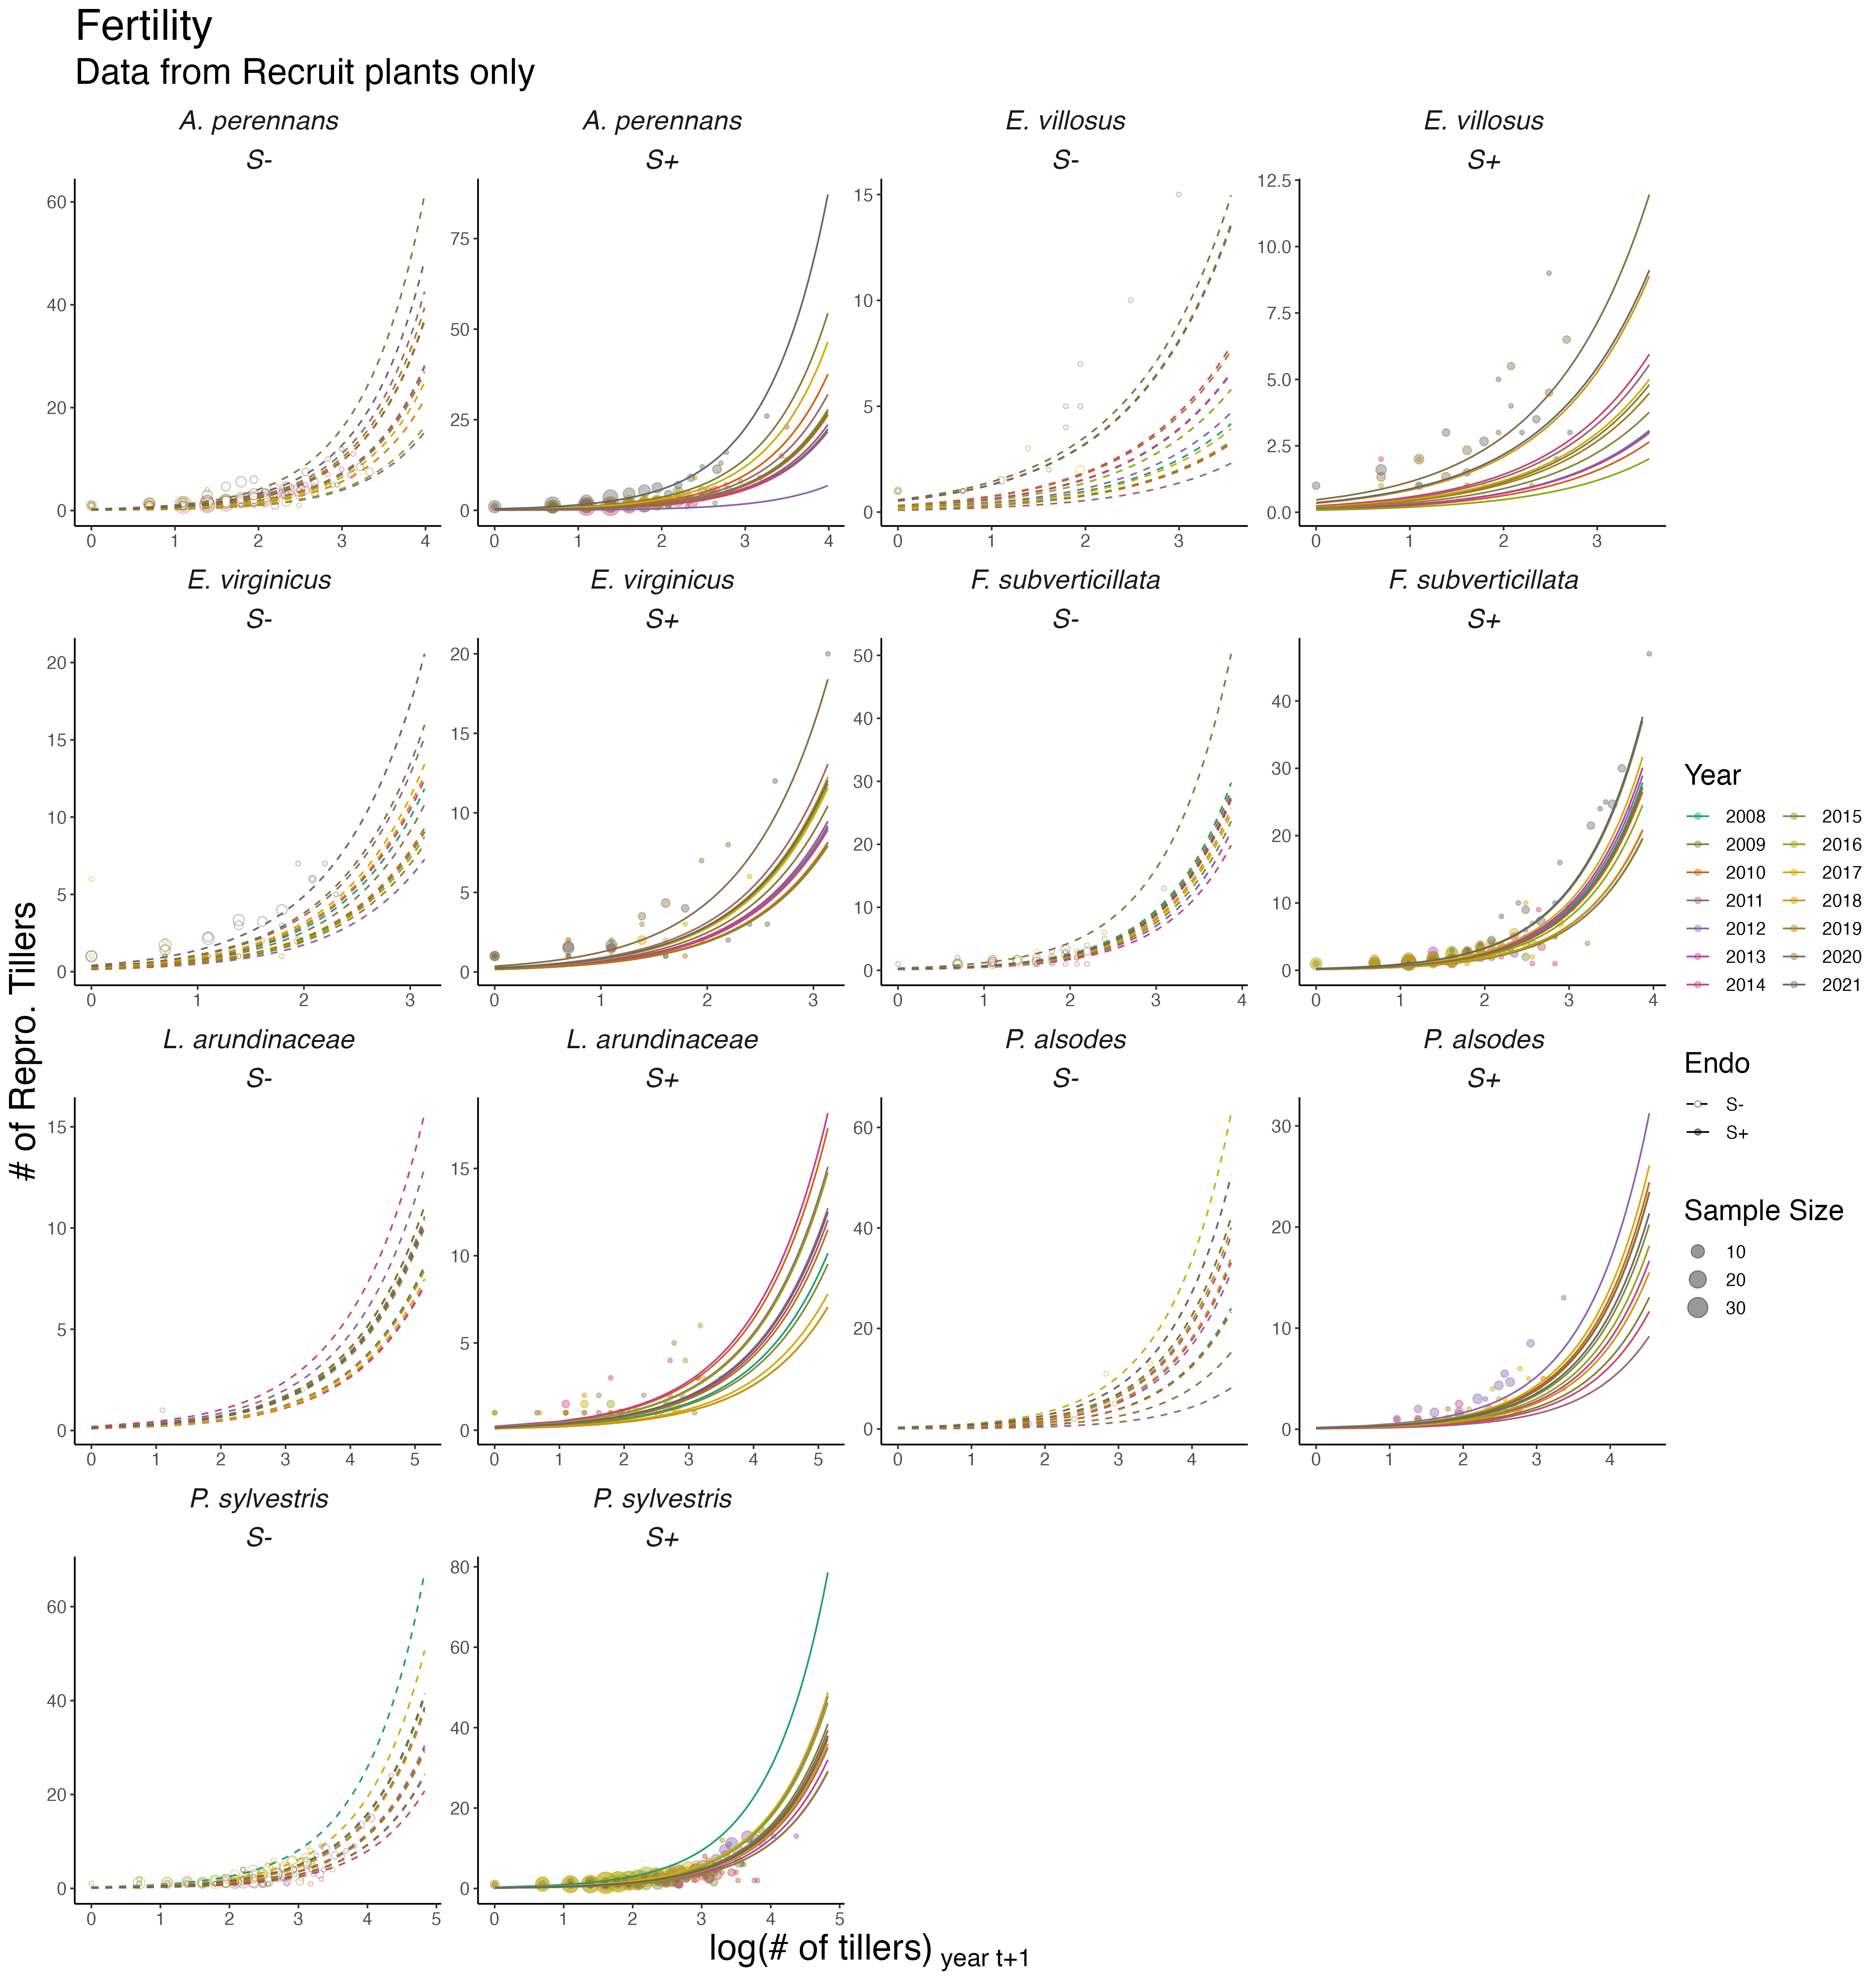
\includegraphics[width=\linewidth]{recruit_fert_yearplot.png}
	\caption{Effect of endophyte symbiosis on yearly fertility. Fitted curves represent the size-specific annual expected number of flowering tillers for recruited along with data binned by size and census year shown as open circles with a dashed line for symbiont-free (S-) plants, while the solid line and filled circles represent symbiontic (S+) plants.}
\end{figure}


\begin{figure}[H]
	\centering
	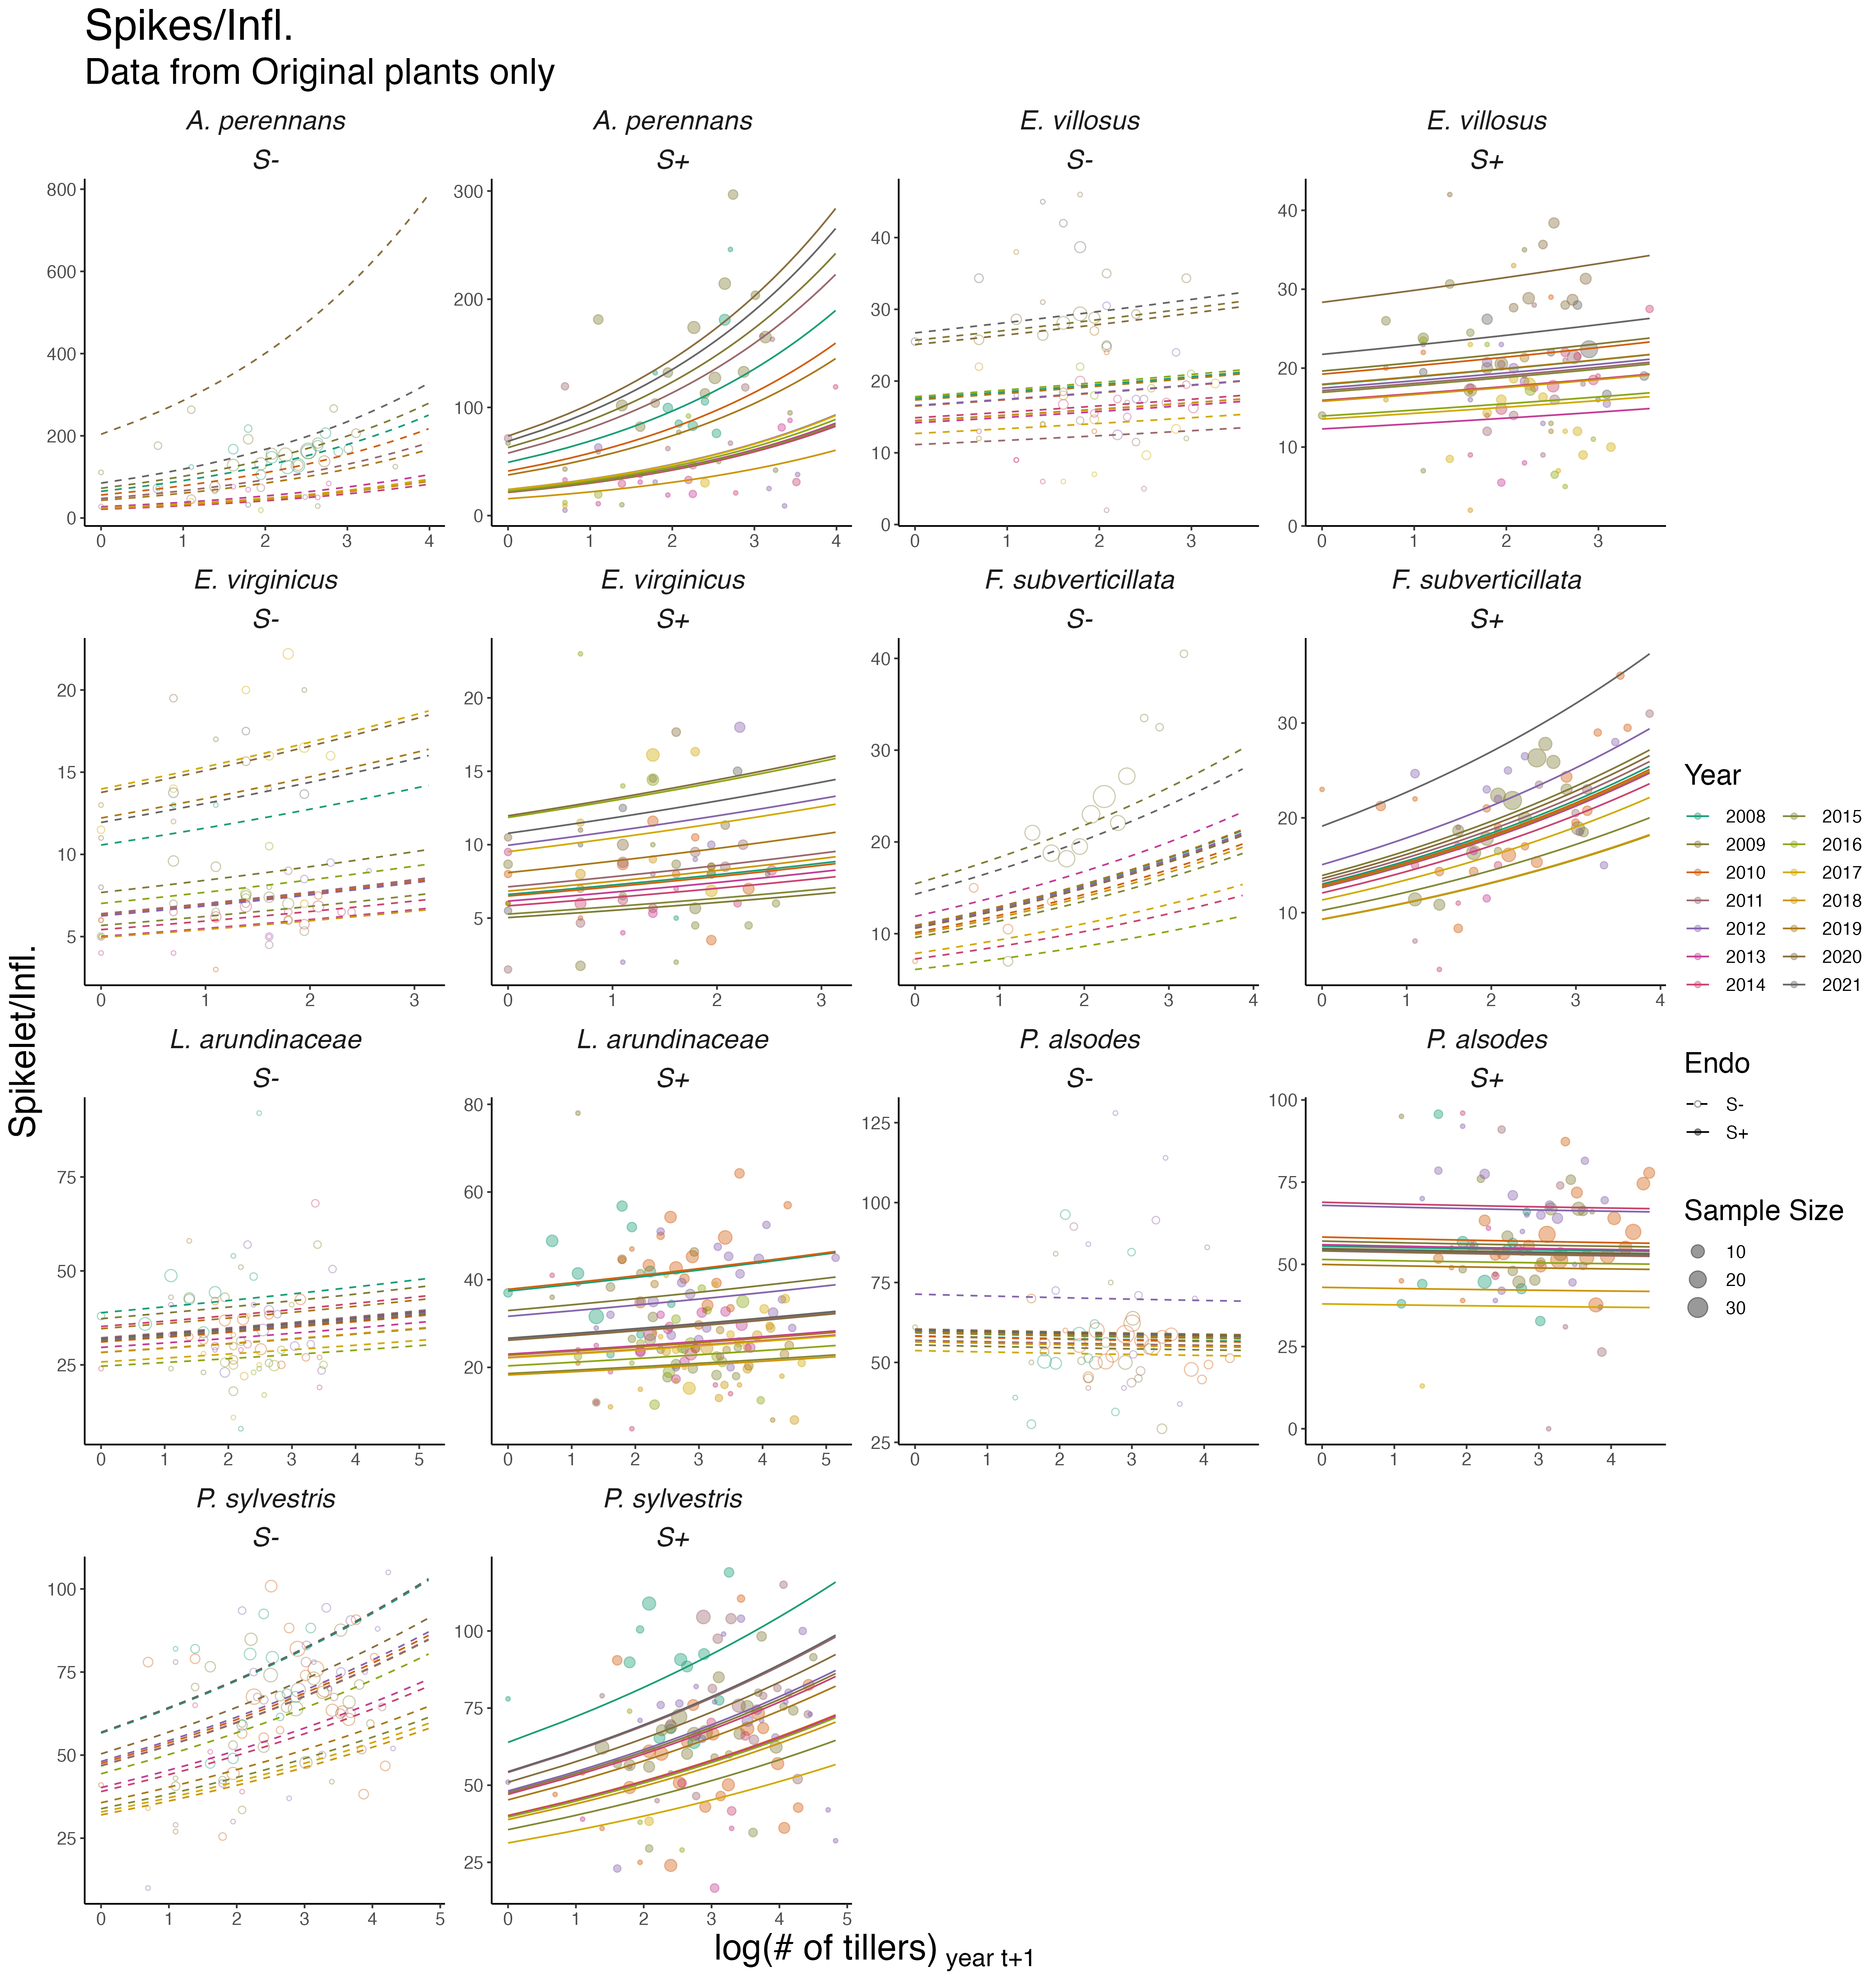
\includegraphics[width=\linewidth]{spike_yearplot.png}
	\caption{Effect of endophyte symbiosis on yearly spikelet production. Fitted curves represent the size-specific annual expected number of spikelets per inflorescence for original plants along with data binned by size and census year shown as open circles with a dashed line for symbiont-free (S-) plants, while the solid line and filled circles represent symbiontic (S+) plants.}
\end{figure}


\begin{figure}[H]
	\centering
	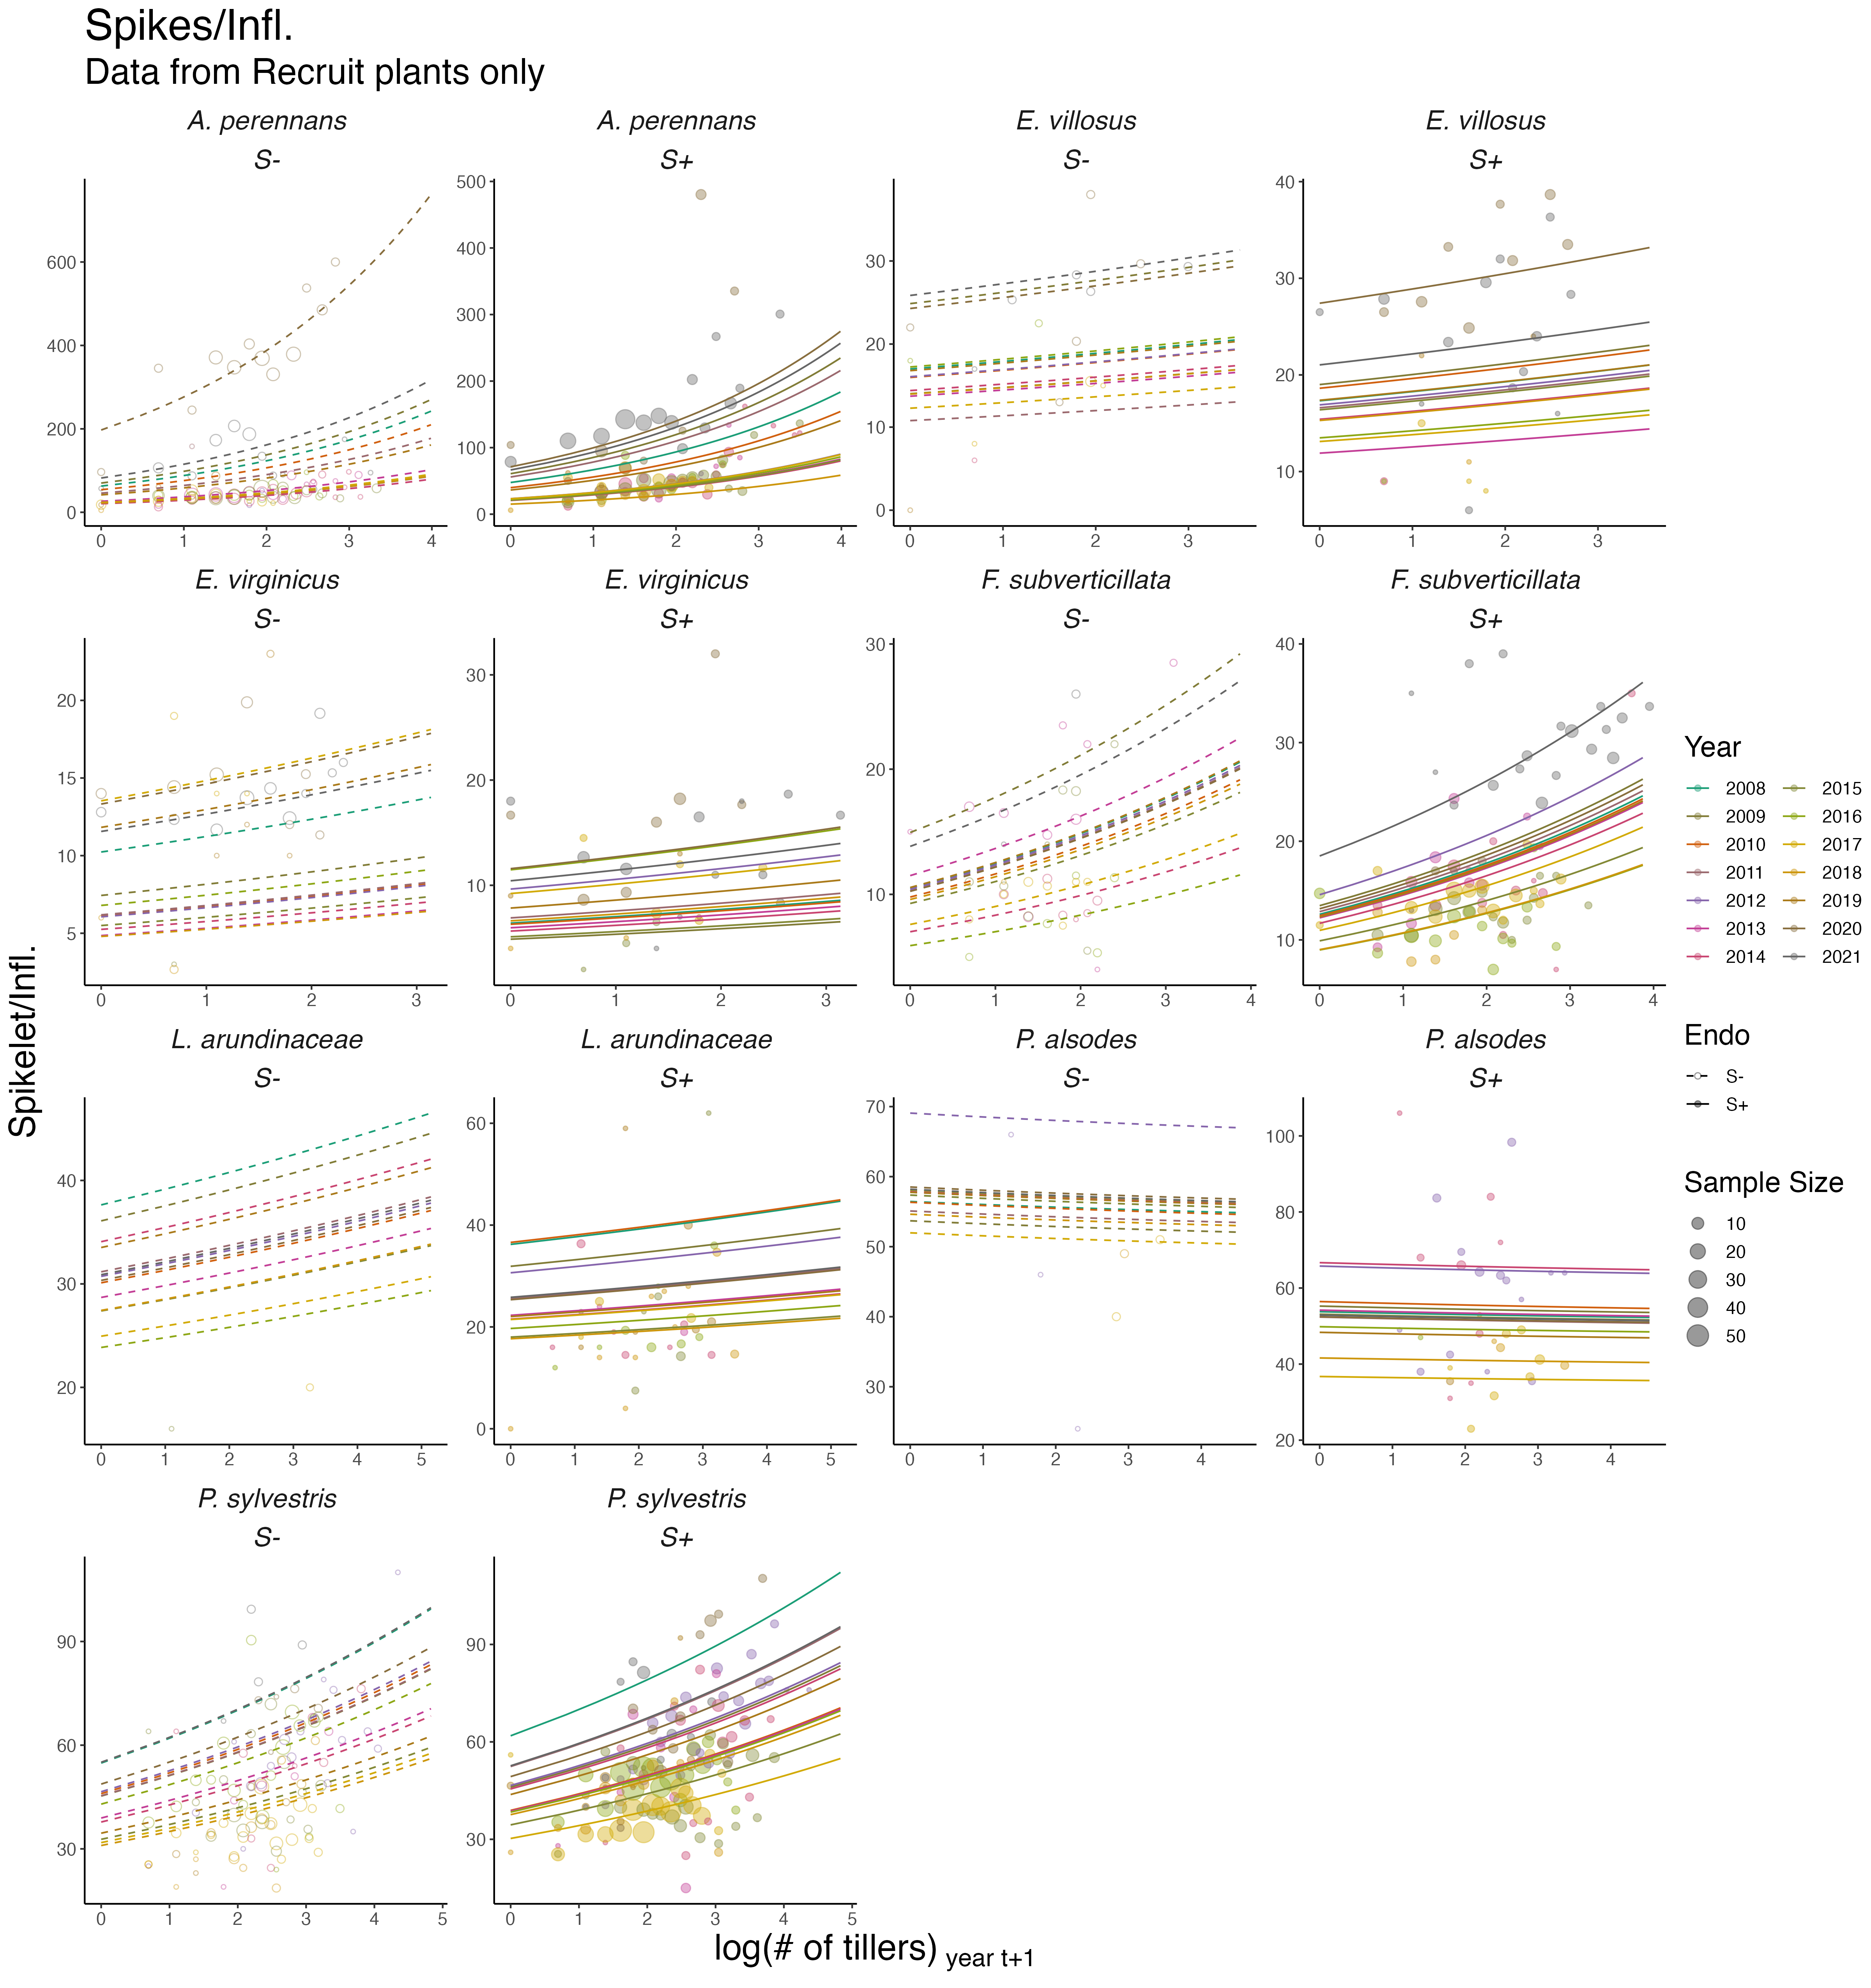
\includegraphics[width=\linewidth]{recruit_spike_yearplot.png}
	\caption{Effect of endophyte symbiosis on yearly spikelet production. Fitted curves represent the size-specific annual expected number of spikelets per inflorescence for recruited plants along with data binned by size and census year shown as open circles with a dashed line for symbiont-free (S-) plants, while the solid line and filled circles represent symbiontic (S+) plants.}
\end{figure}


\begin{figure}[H]
	\centering
	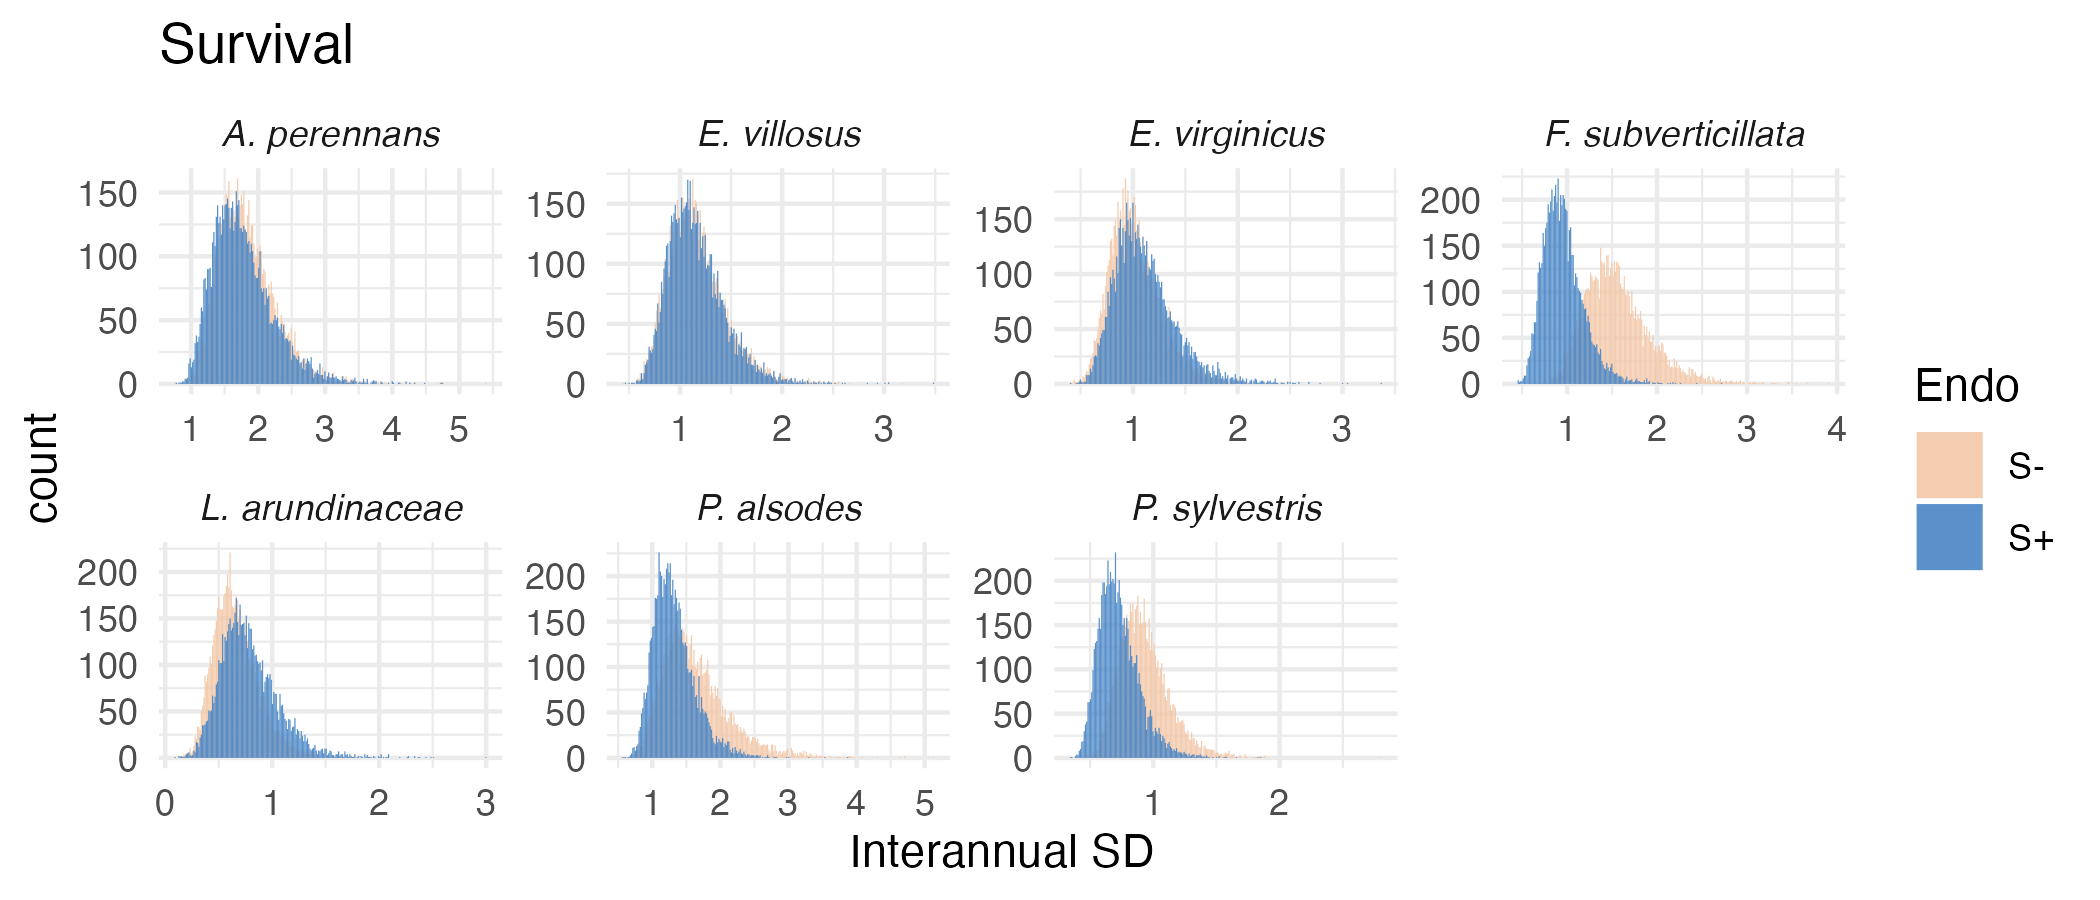
\includegraphics[width=.9\linewidth]{surv_sigmayear_hist.png}
	\caption{Posterior distributions of the standard deviations of inter-annual year effects for survival. Histograms include 7500 post-warmup MCMC samples for symbiotic (S+; blue) and symbiont-free (S-; tan) plants from fitted vital rate model.}
\end{figure}


\begin{figure}[H]
	\centering
	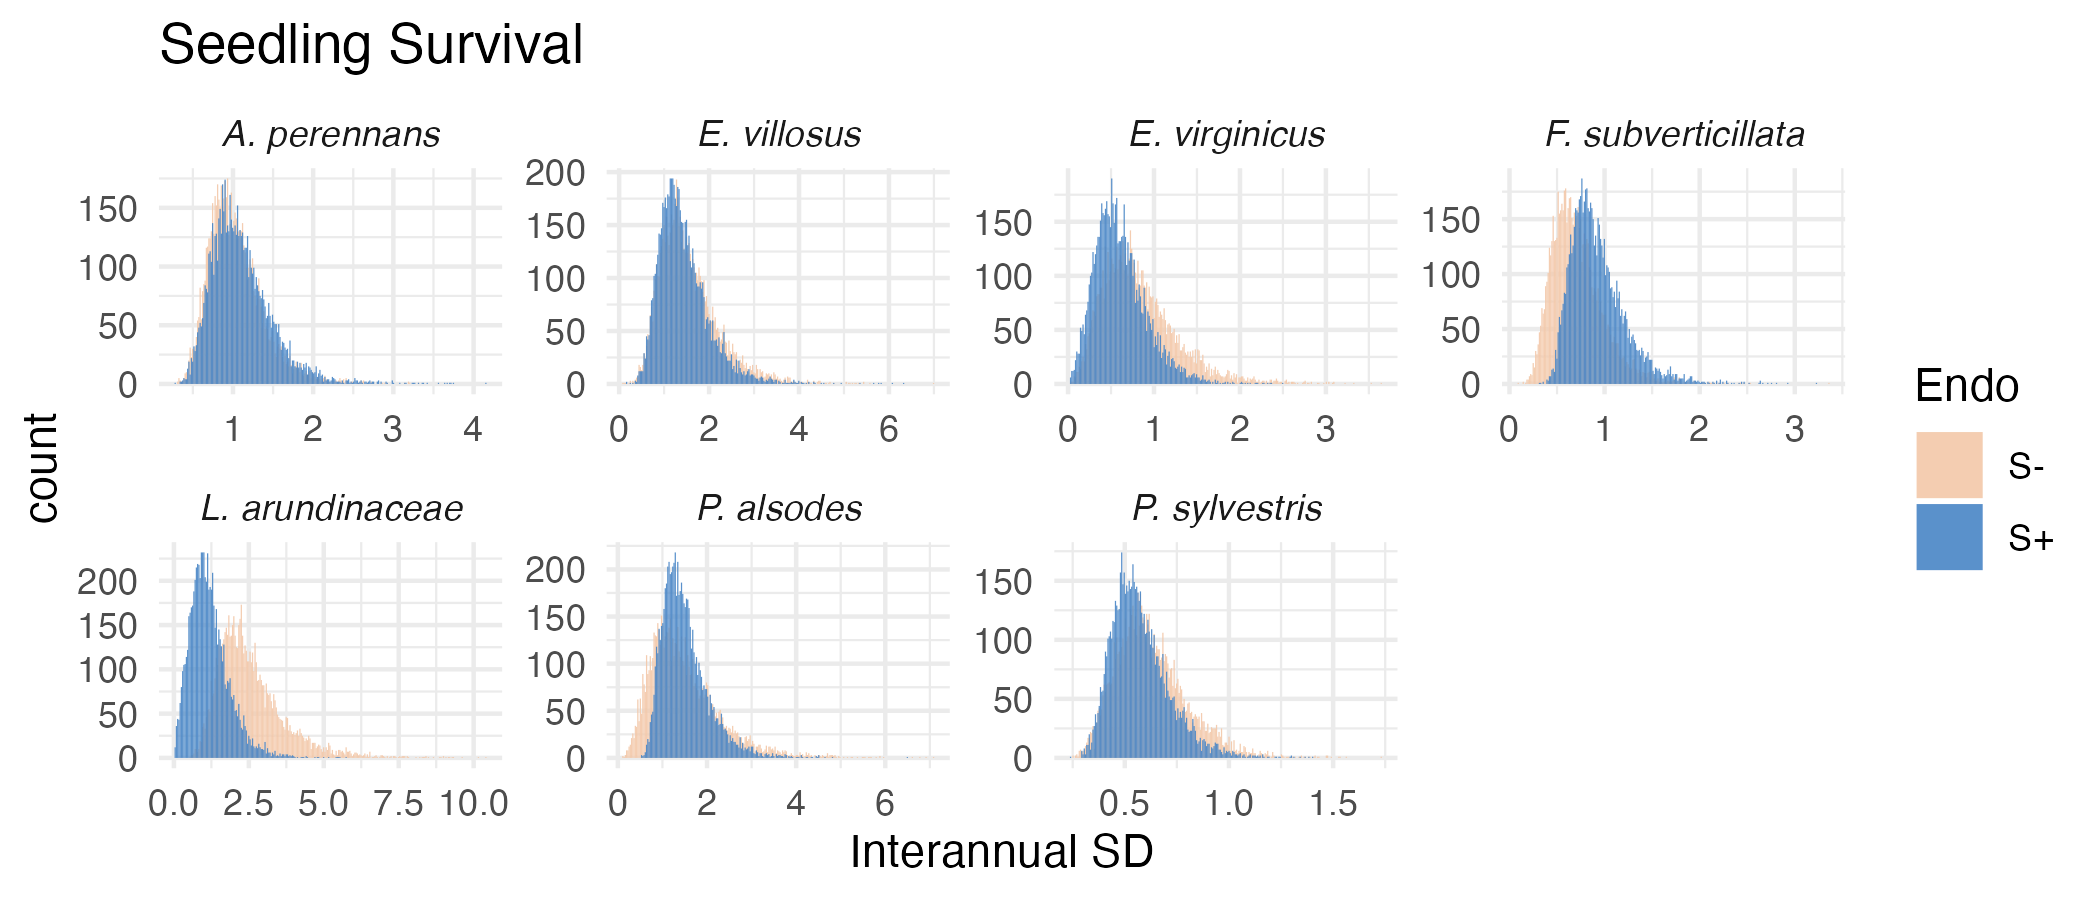
\includegraphics[width=.9\linewidth]{seedsurv_sigmayear_hist.png}
	\caption{Posterior distributions of the standard deviations of inter-annual year effects for seedling survival. Histograms include 7500 post-warmup MCMC samples for symbiotic (S+; blue) and symbiont-free (S-; tan) plants from fitted vital rate model.}
\end{figure}


\begin{figure}[H]
	\centering
	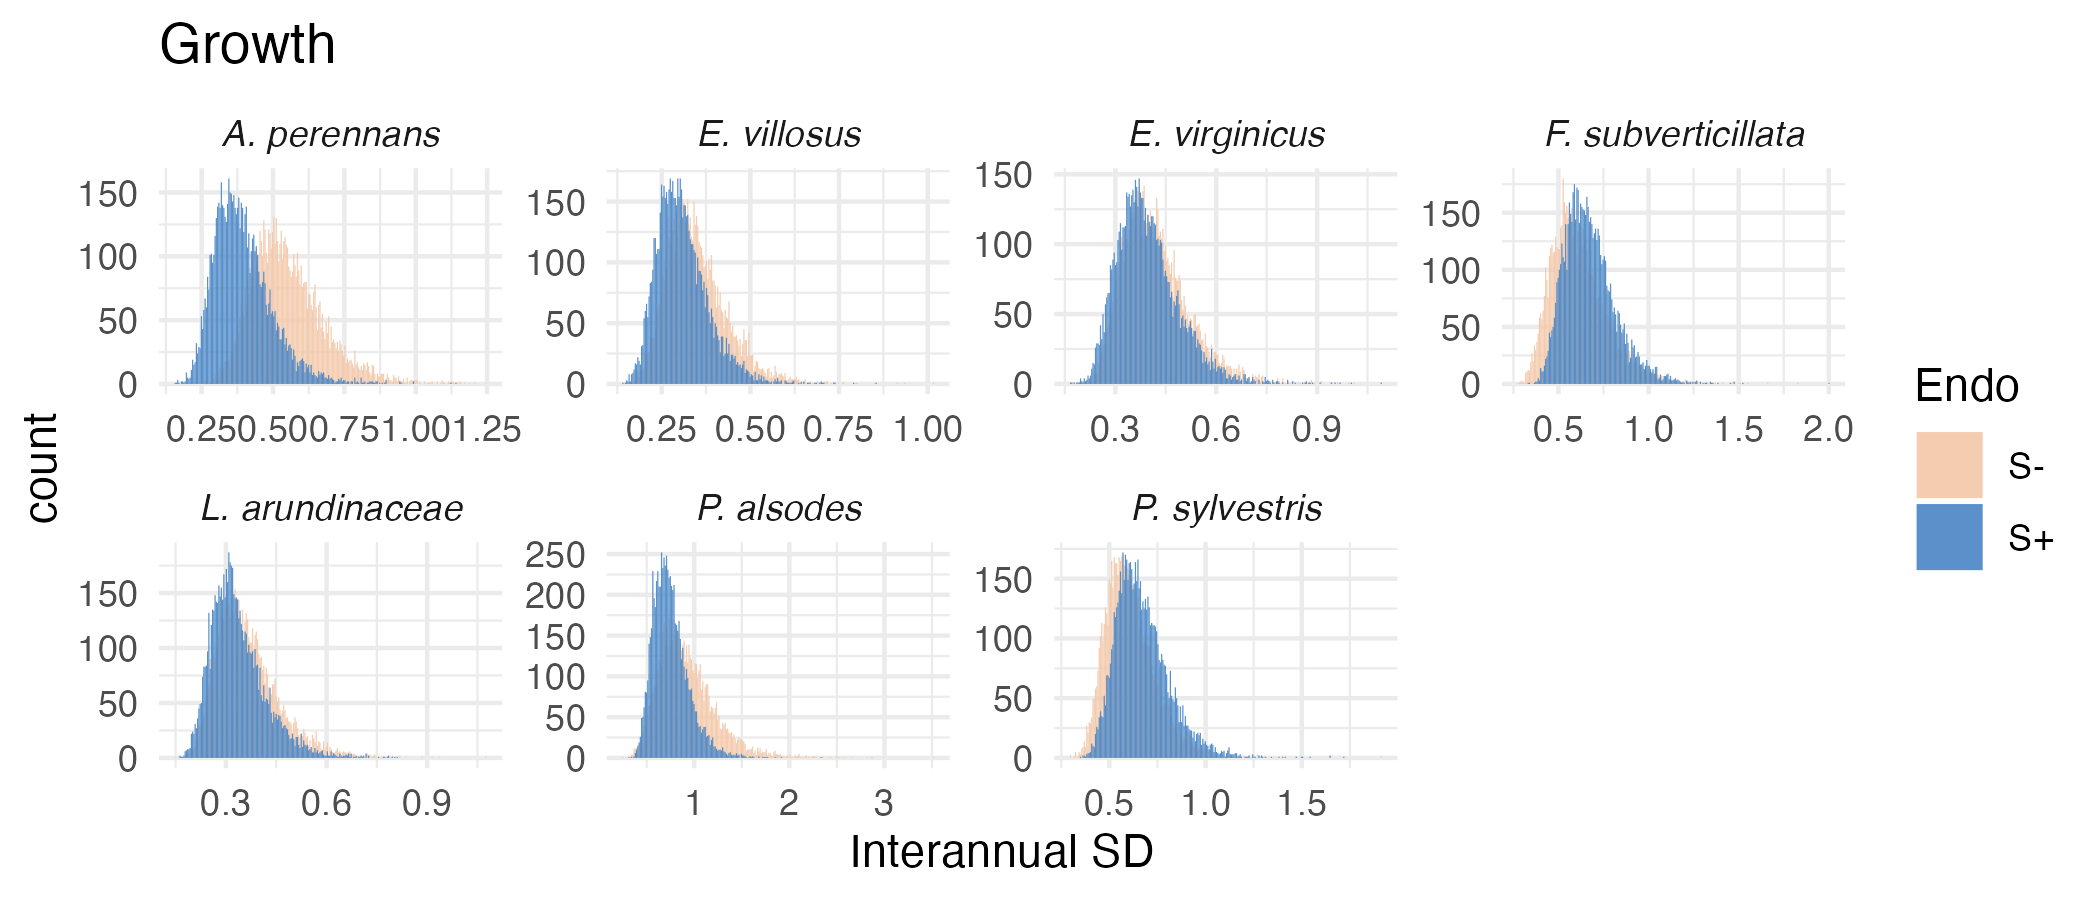
\includegraphics[width=.9\linewidth]{grow_sigmayear_hist.png}
	\caption{Posterior distributions of the standard deviations of inter-annual year effects for growth. Histograms include 7500 post-warmup MCMC samples for symbiotic (S+; blue) and symbiont-free (S-; tan) plants from fitted vital rate model.}
\end{figure}


\begin{figure}[H]
	\centering
	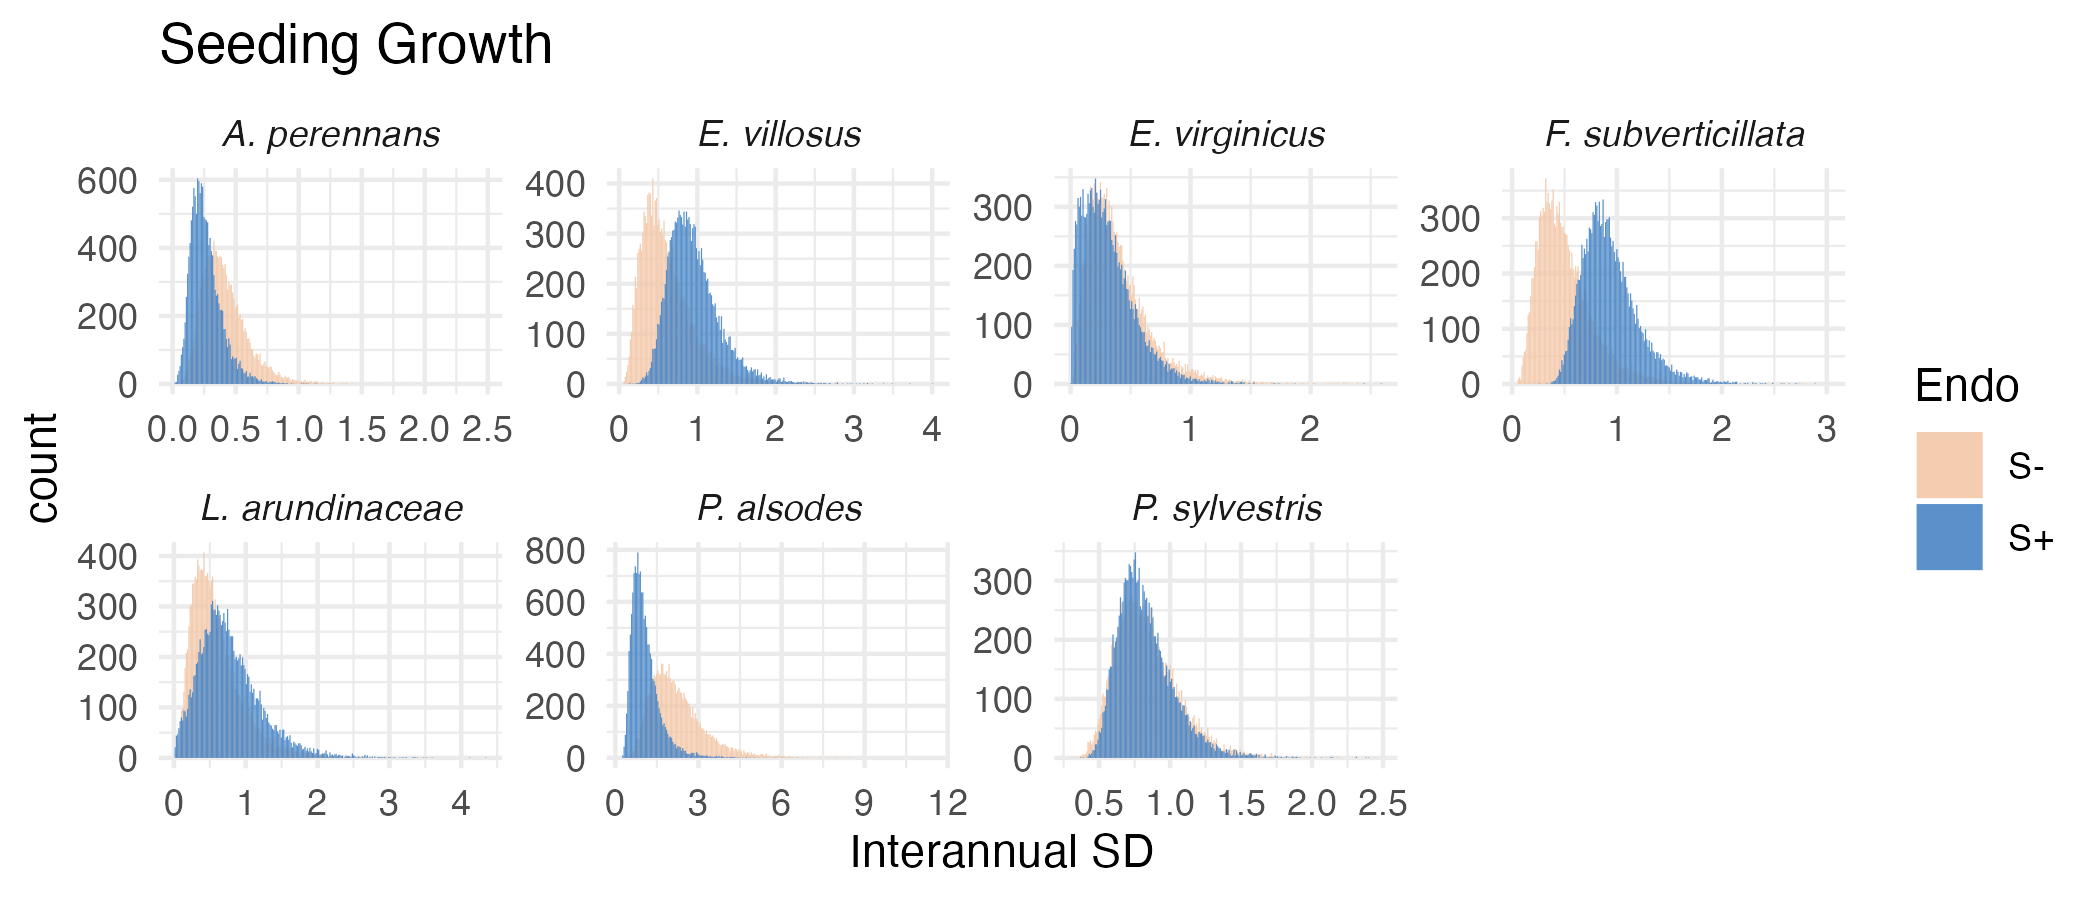
\includegraphics[width=.9\linewidth]{seedgrow_sigmayear_hist.png}
	\caption{Posterior distributions of the standard deviations of inter-annual year effects for seedling growth. Histograms include 7500 post-warmup MCMC samples for symbiotic (S+; blue) and symbiont-free (S-; tan) plants from fitted vital rate model.}
\end{figure}


\begin{figure}[H]
	\centering
	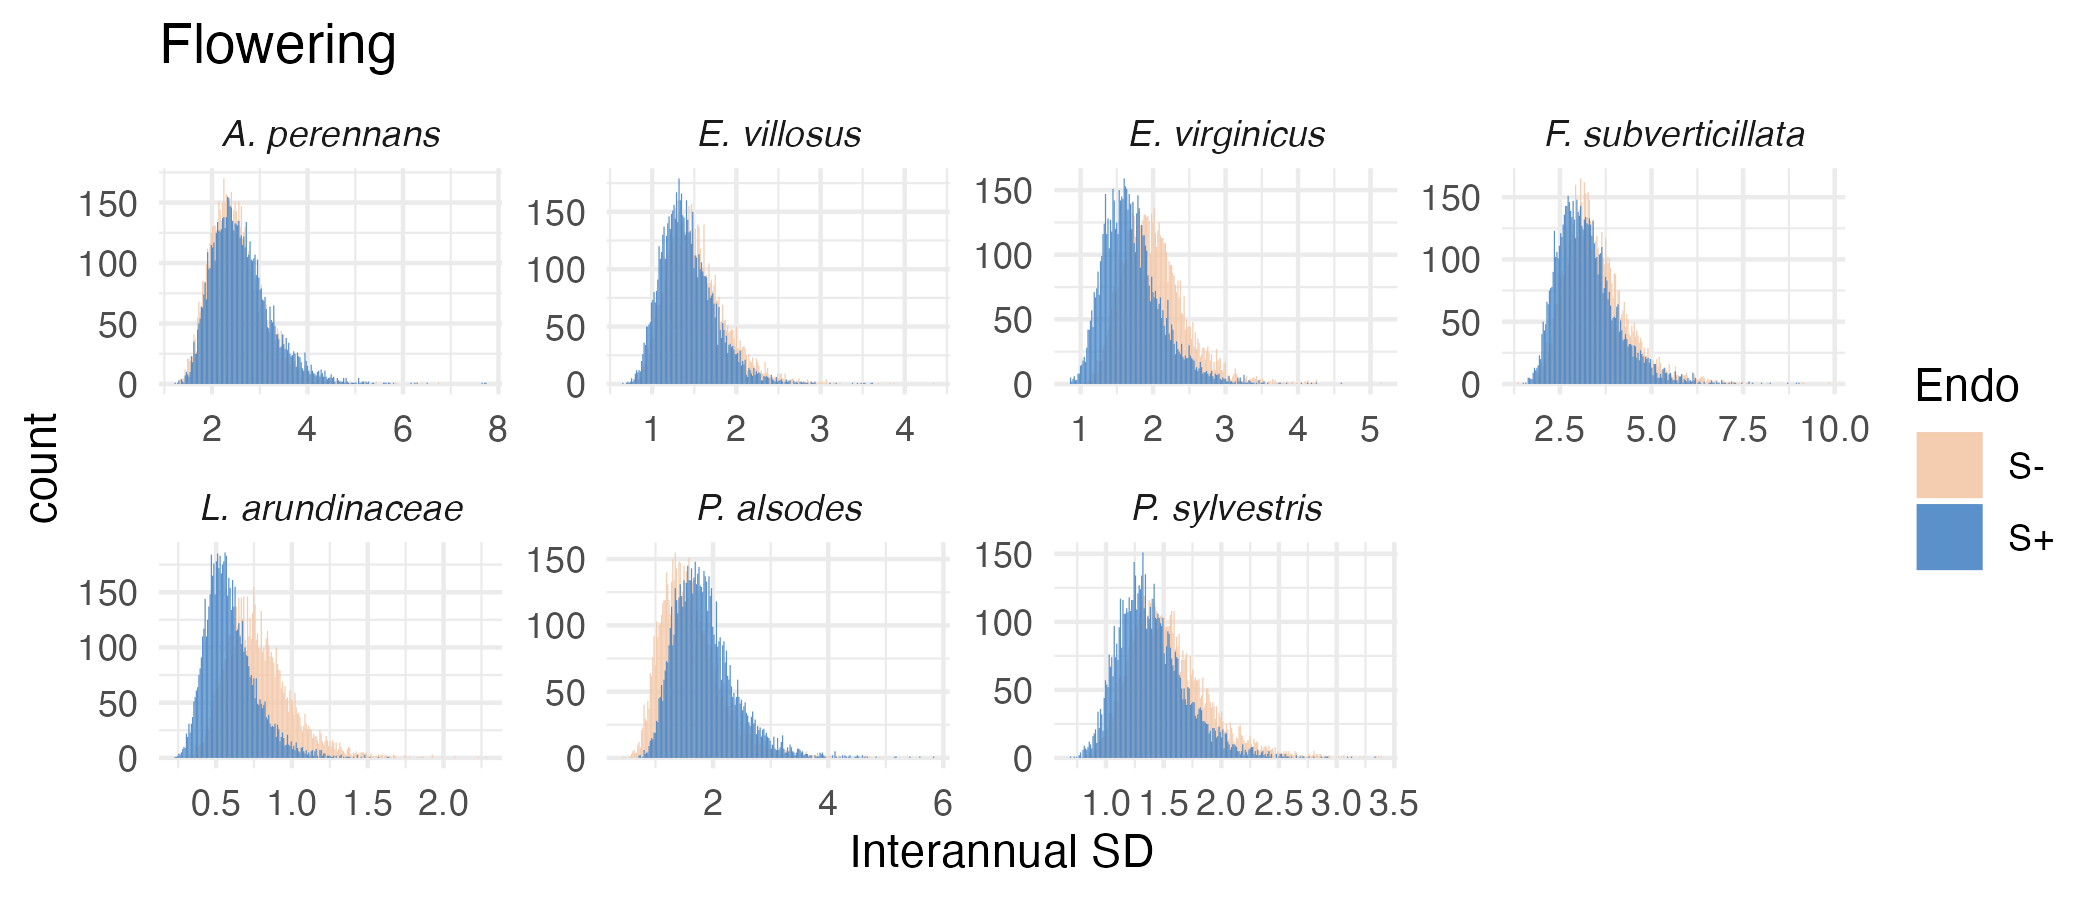
\includegraphics[width=.9\linewidth]{flow_sigmayear_hist.png}
	\caption{Posterior distributions of the standard deviations of inter-annual year effects for flowering probability. Histograms include 7500 post-warmup MCMC samples for symbiotic (S+; blue) and symbiont-free (S-; tan) plants from fitted vital rate model.}
\end{figure}


\begin{figure}[H]
	\centering
	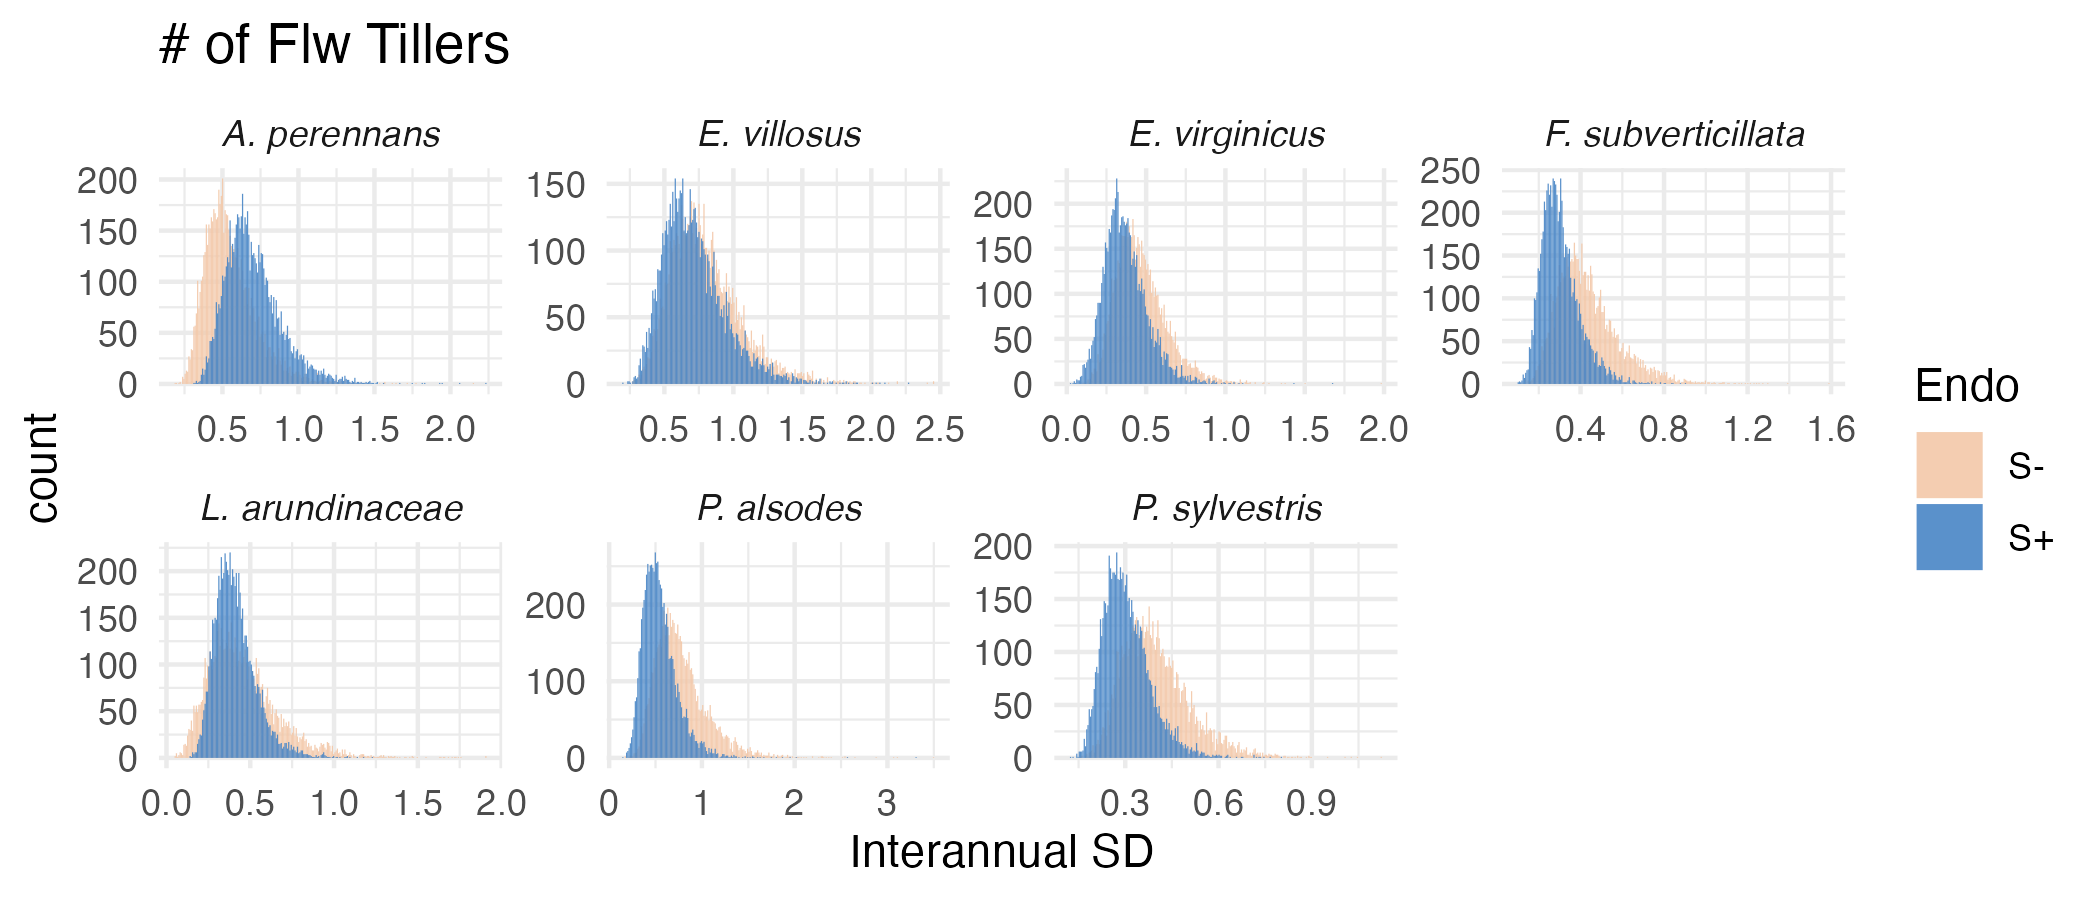
\includegraphics[width=.9\linewidth]{fert_sigmayear_hist.png}
	\caption{Posterior distributions of the standard deviations of inter-annual year effects for fertility (no. of flowering tillers). Histograms include 7500 post-warmup MCMC samples for symbiotic (S+; blue) and symbiont-free (S-; tan) plants from fitted vital rate model.}
\end{figure}


\begin{figure}[H]
	\centering
	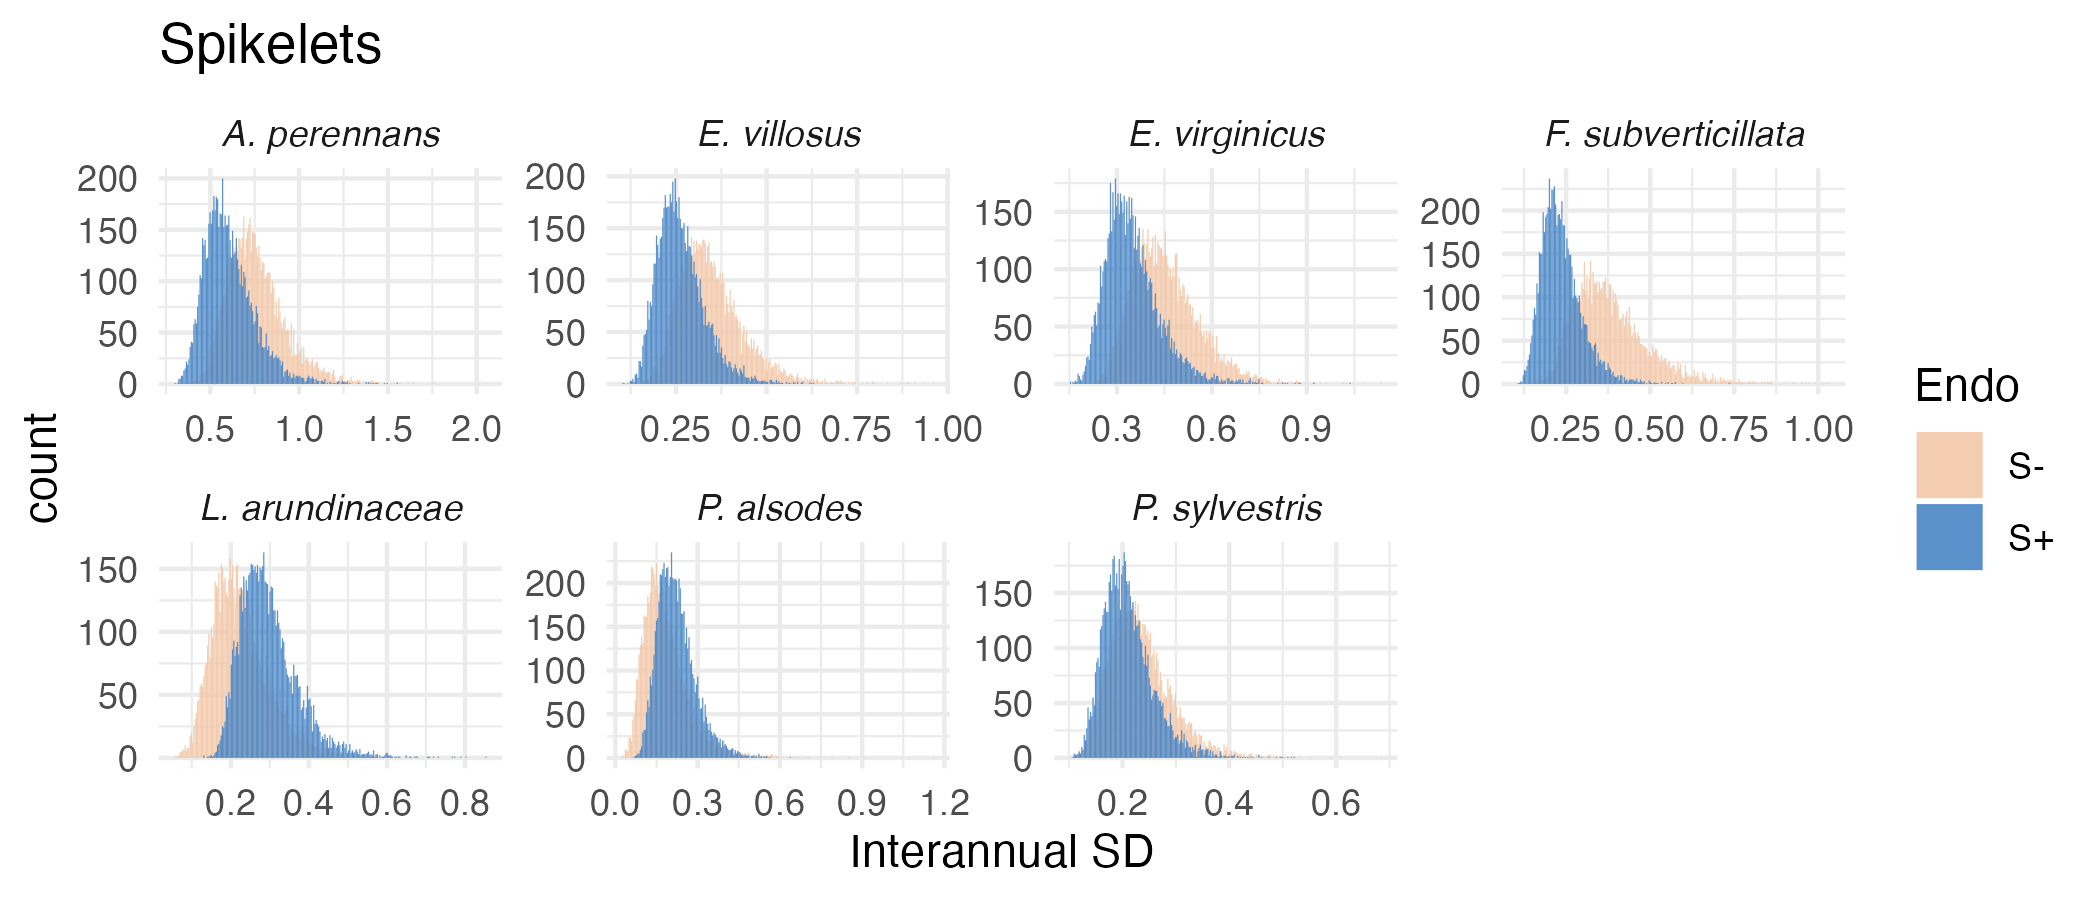
\includegraphics[width=.9\linewidth]{spike_sigmayear_hist.png}
	\caption{Posterior distributions of the standard deviations of inter-annual year effects for spikelets per inflorescence. Histograms include 7500 post-warmup MCMC samples for symbiotic (S+; blue) and symbiont-free (S-; tan) plants from fitted vital rate model.}
\end{figure}


\begin{figure}[H]
	\centering
	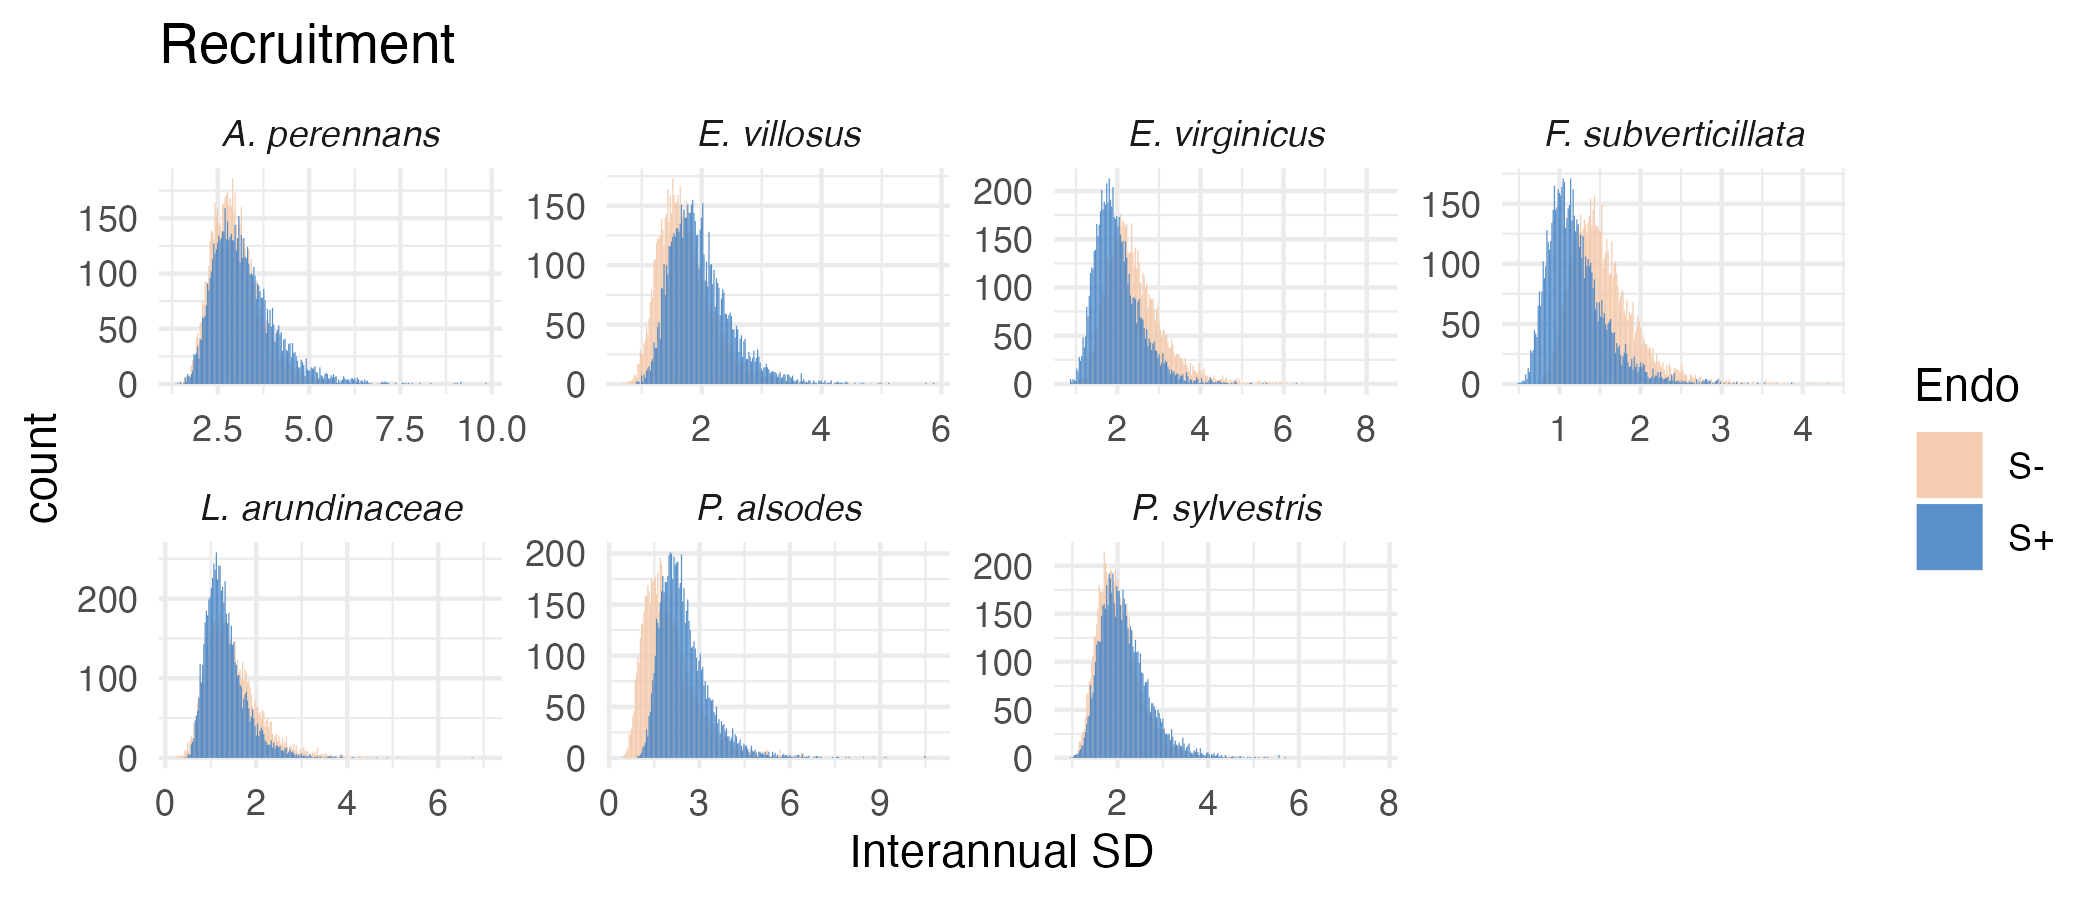
\includegraphics[width=.9\linewidth]{recruit_sigmayear_hist.png}
	\caption{Posterior distributions of the standard deviations of inter-annual year effects for recruitment. Histograms include 7500 post-warmup MCMC samples for symbiotic (S+; blue) and symbiont-free (S-; tan) plants from fitted vital rate model.}
\end{figure}


\begin{figure}[H]
	\centering
	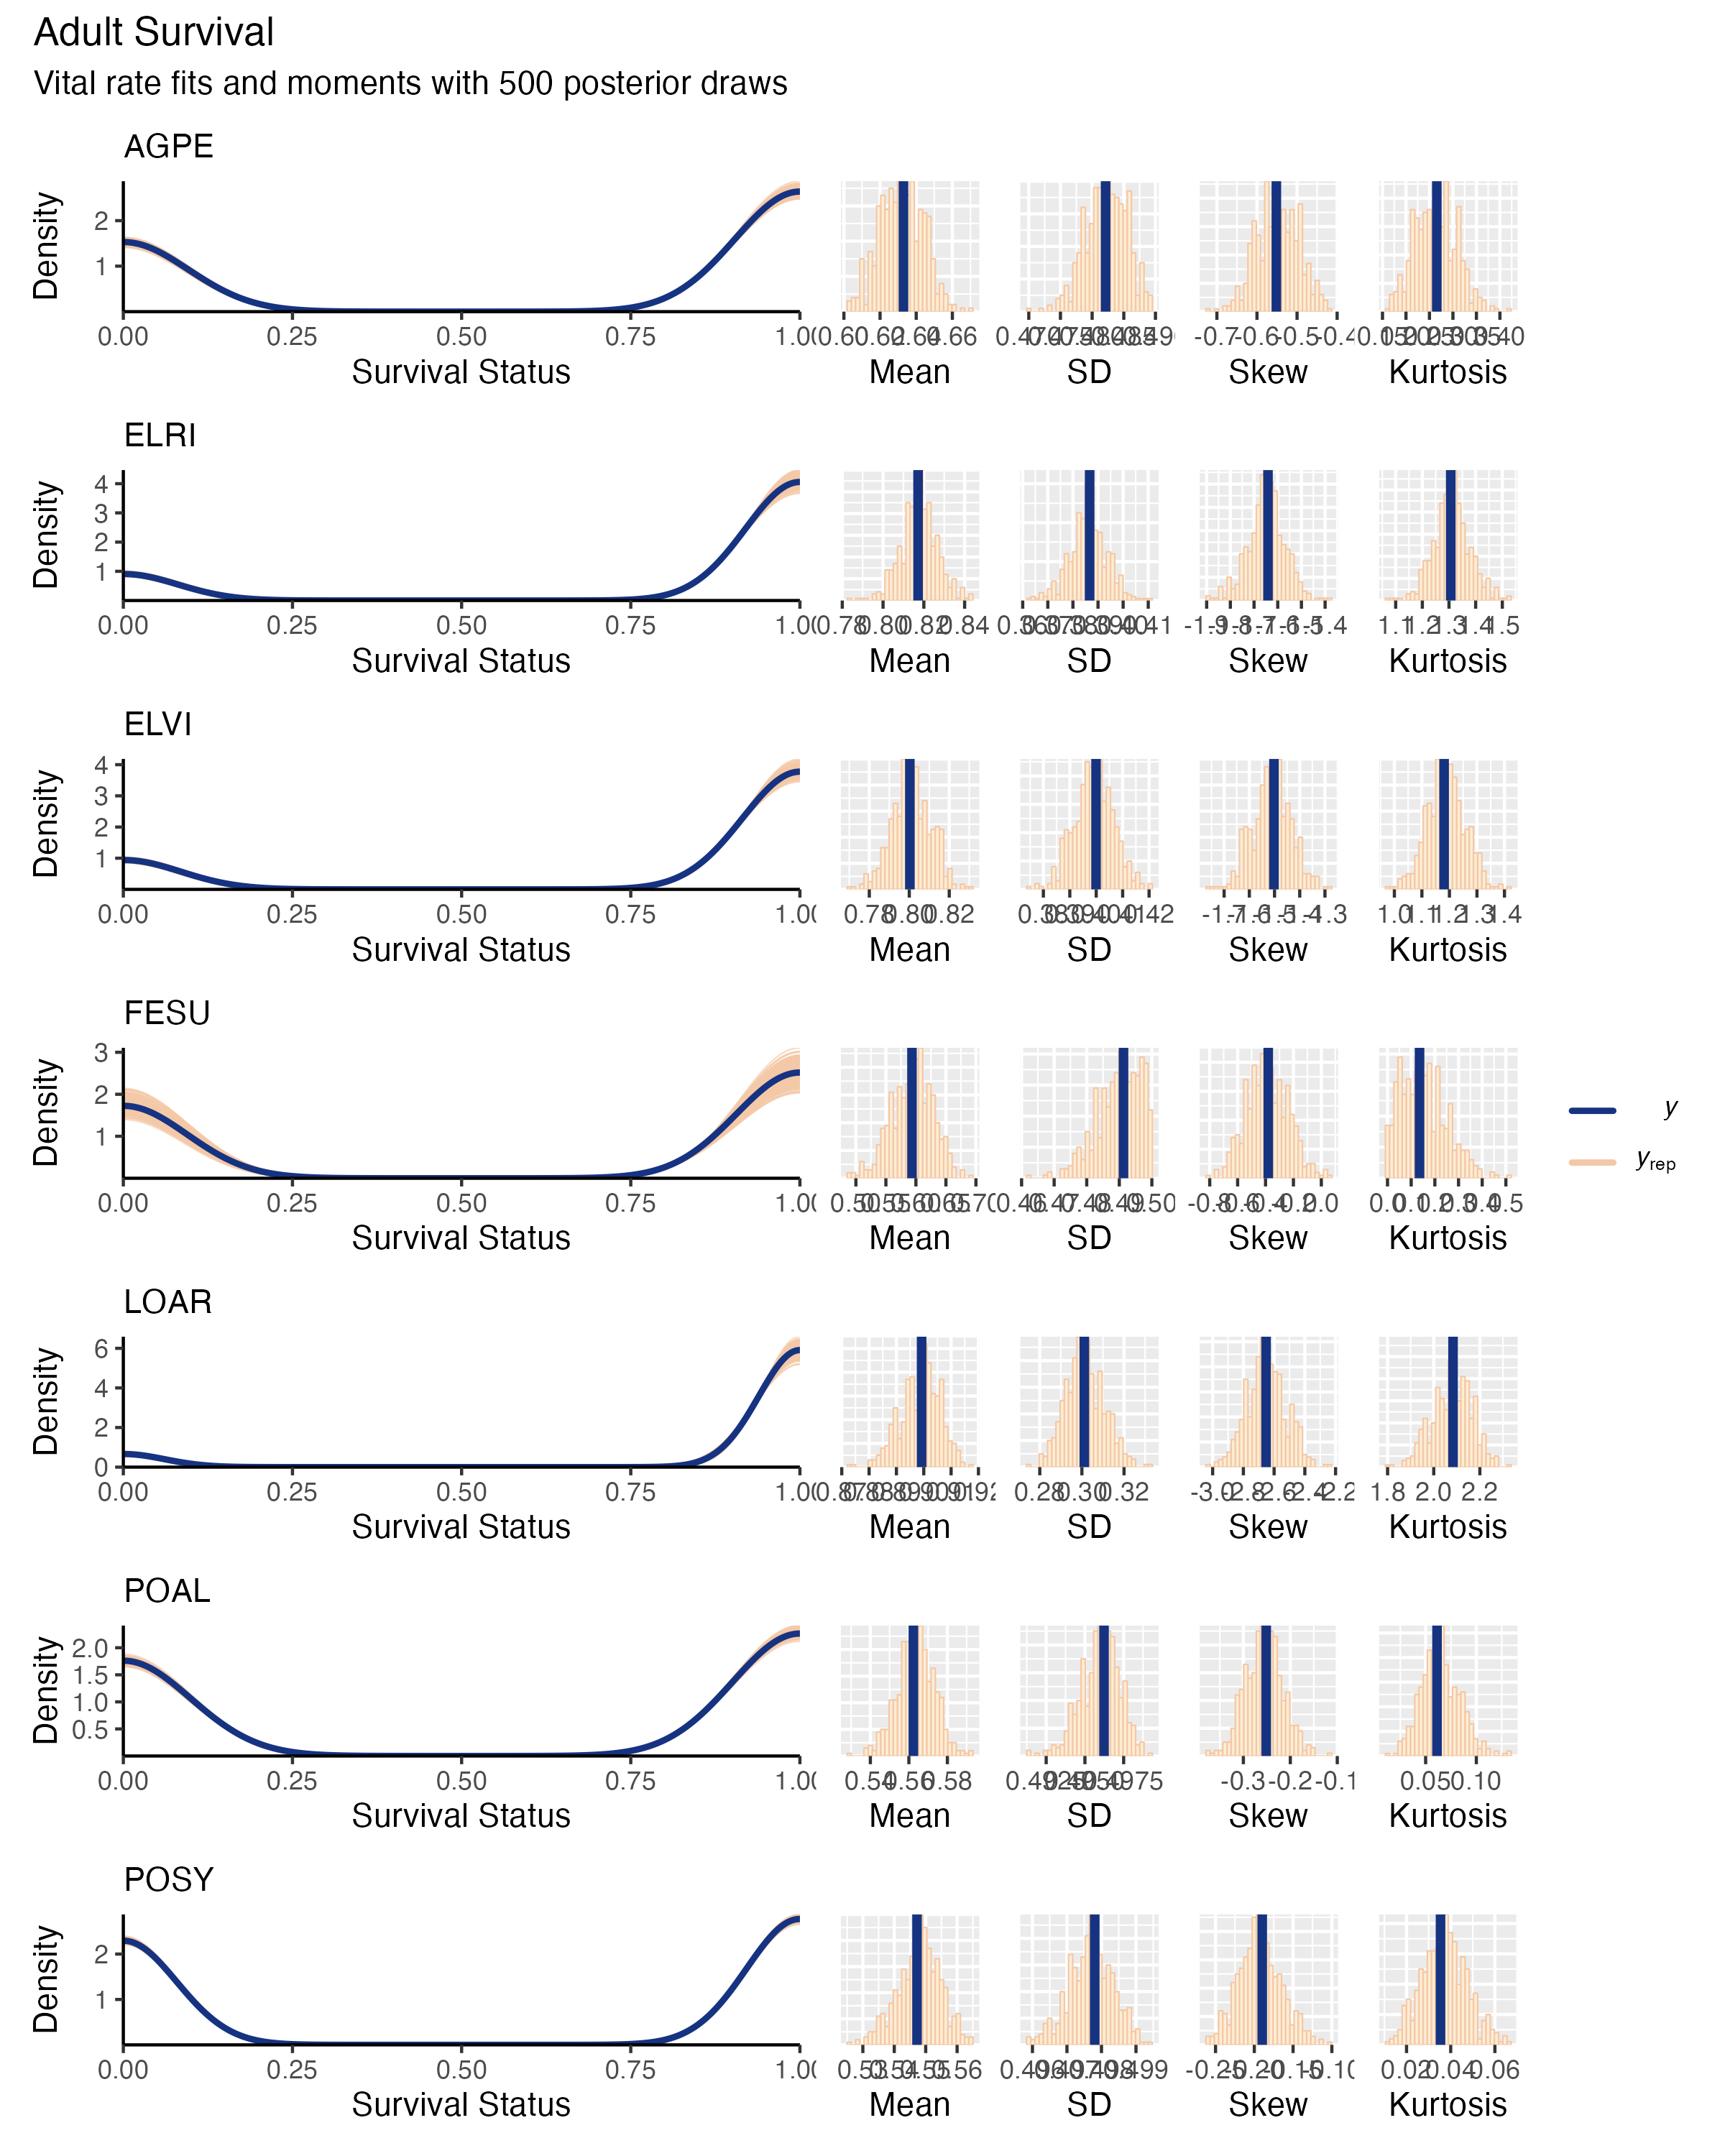
\includegraphics[width = \linewidth]{survbyspecies_densplot.png}
	\caption{Posterior predictive check for statistical model of Adult Survival. Consistency between real data and simulated values indicates that fitted models describe the data well. Lines show density distributions of observed data (blue line) compared to data simulated from fitted models (tan lines) generated from 500 draws from posterior distributions of model parameters along with the distribution's moments.}
\end{figure}

\begin{figure}[H]
	\centering
	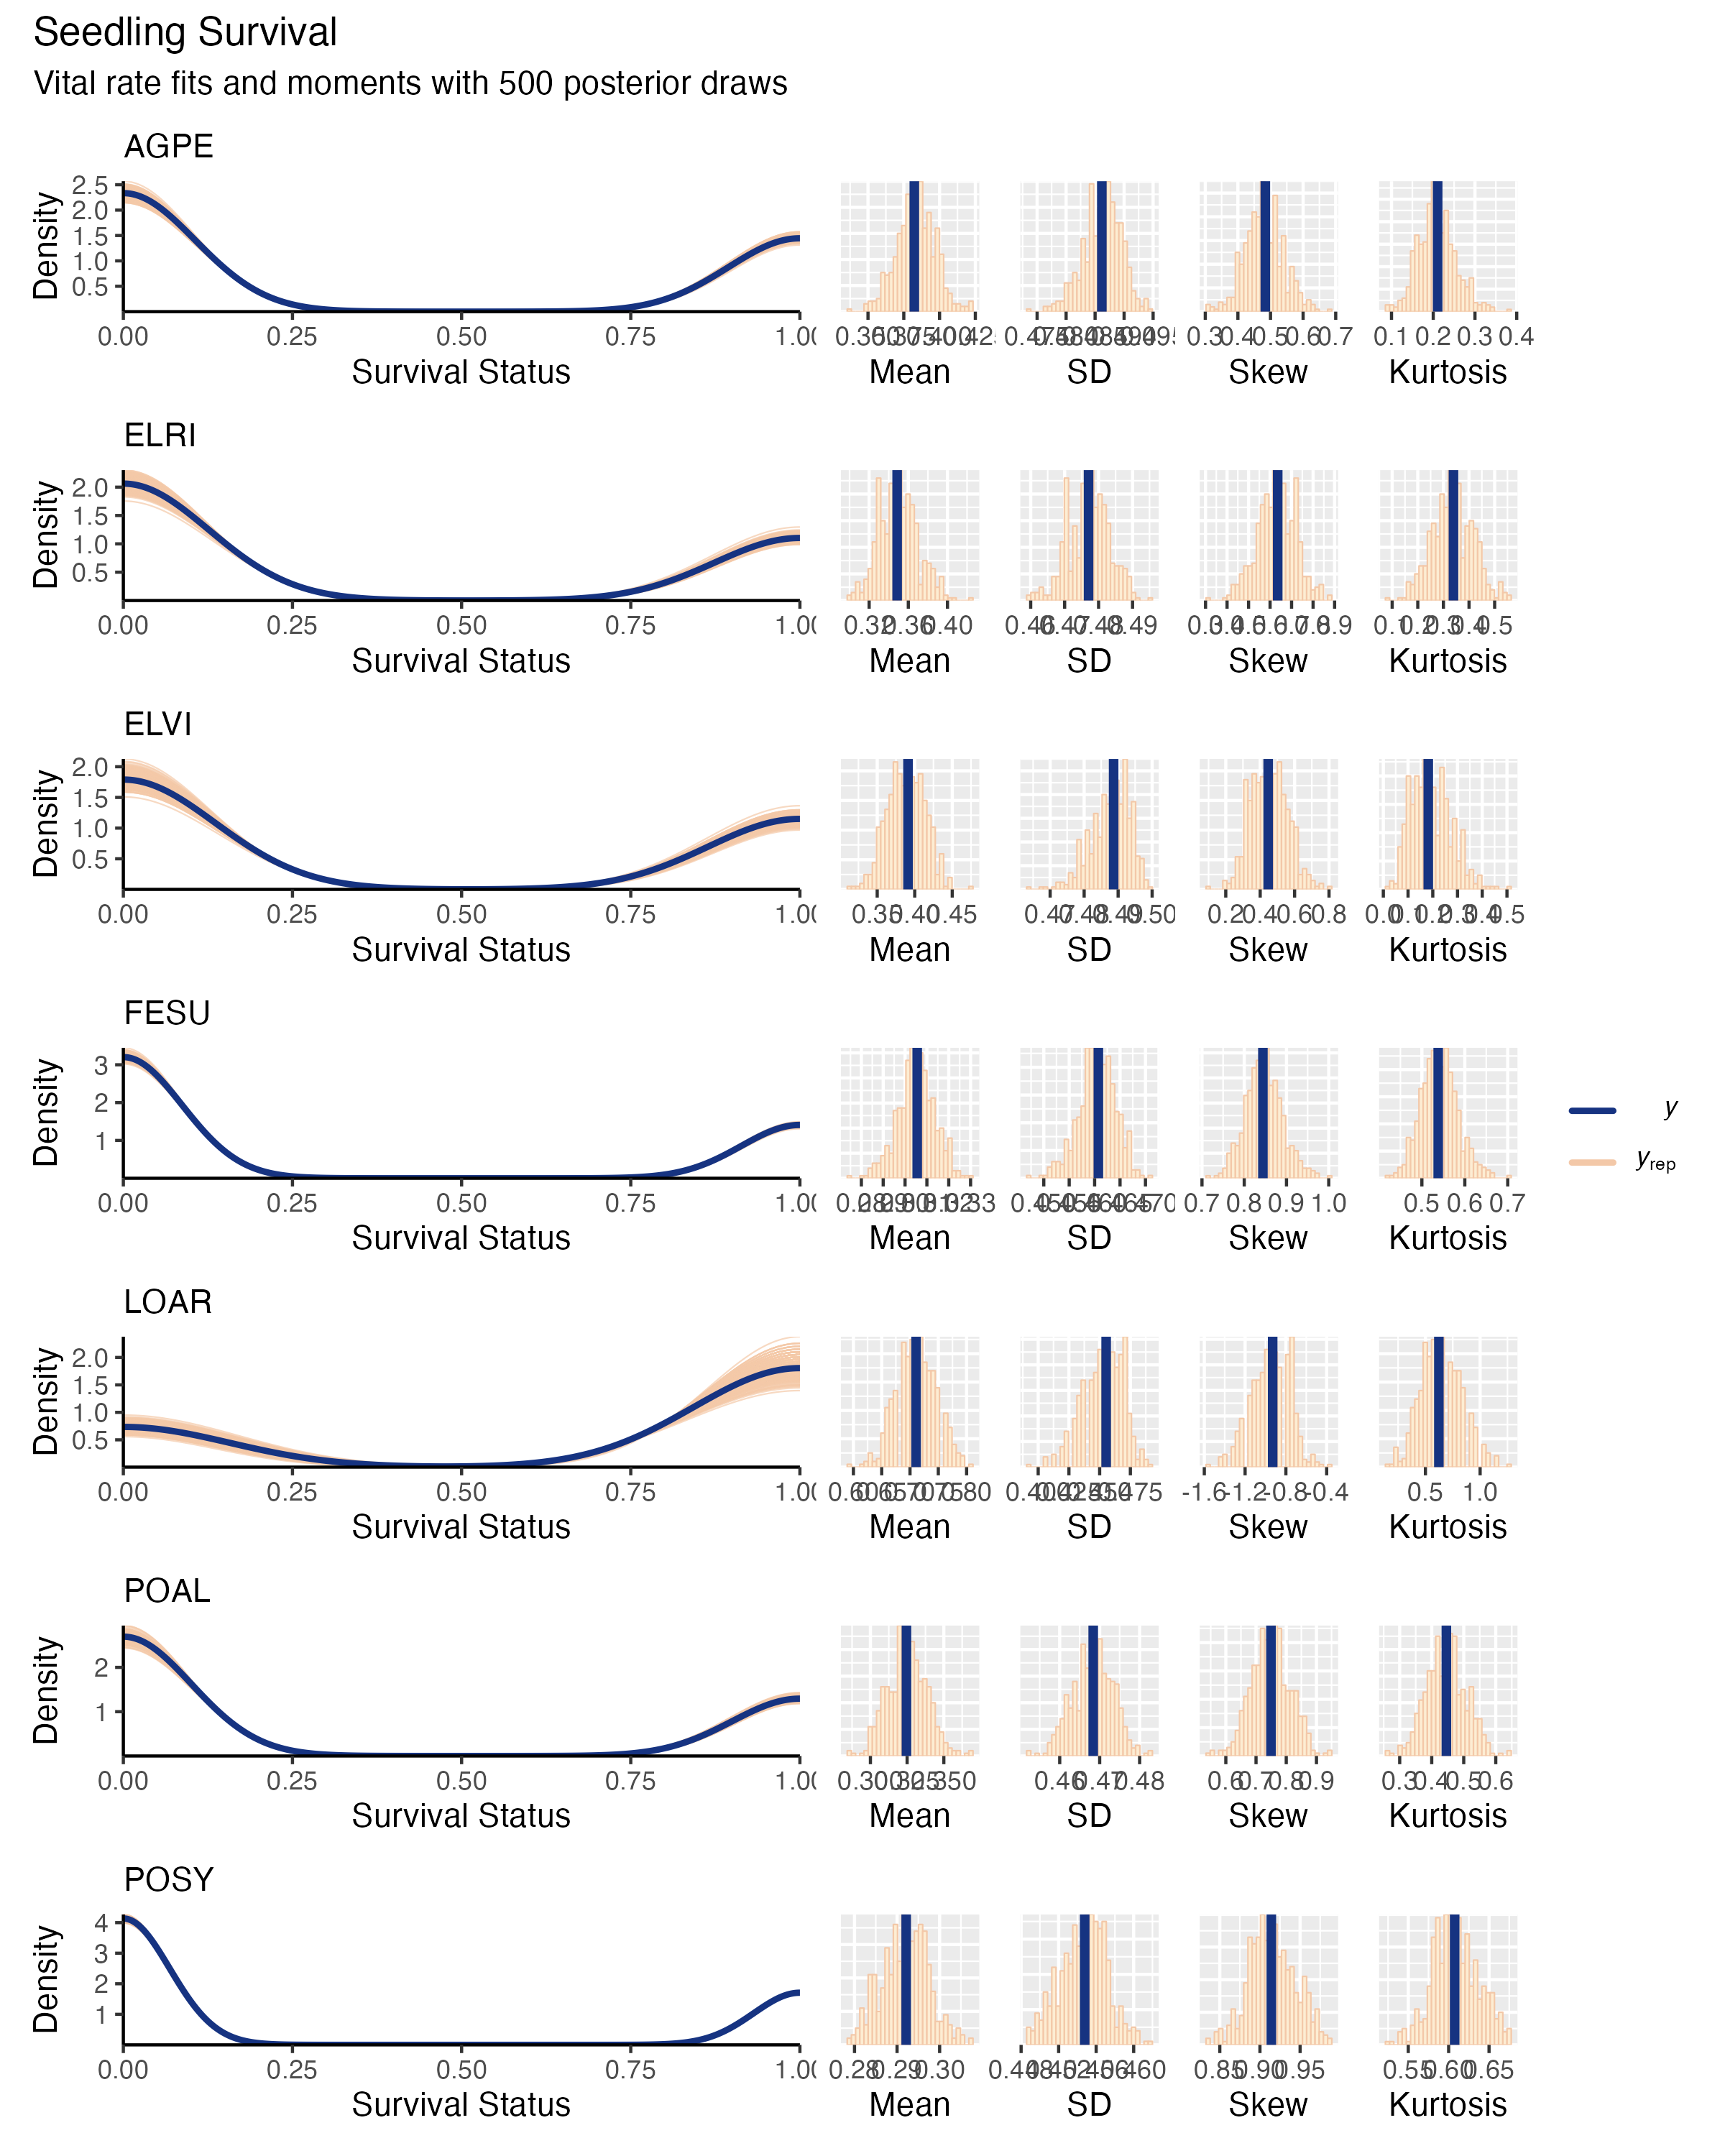
\includegraphics[width = \linewidth]{seedsurvbyspecies_densplot.png}
	\caption{Posterior predictive check for statistical model of Seedling Survival. Consistency between real data and simulated values indicates that fitted models describe the data well. Lines show density distributions of observed data (blue line) compared to data simulated from fitted models (tan lines) generated from 500 draws from posterior distributions of model parameters along with the distribution's moments.}
\end{figure}


\begin{figure}[H]
	\centering
	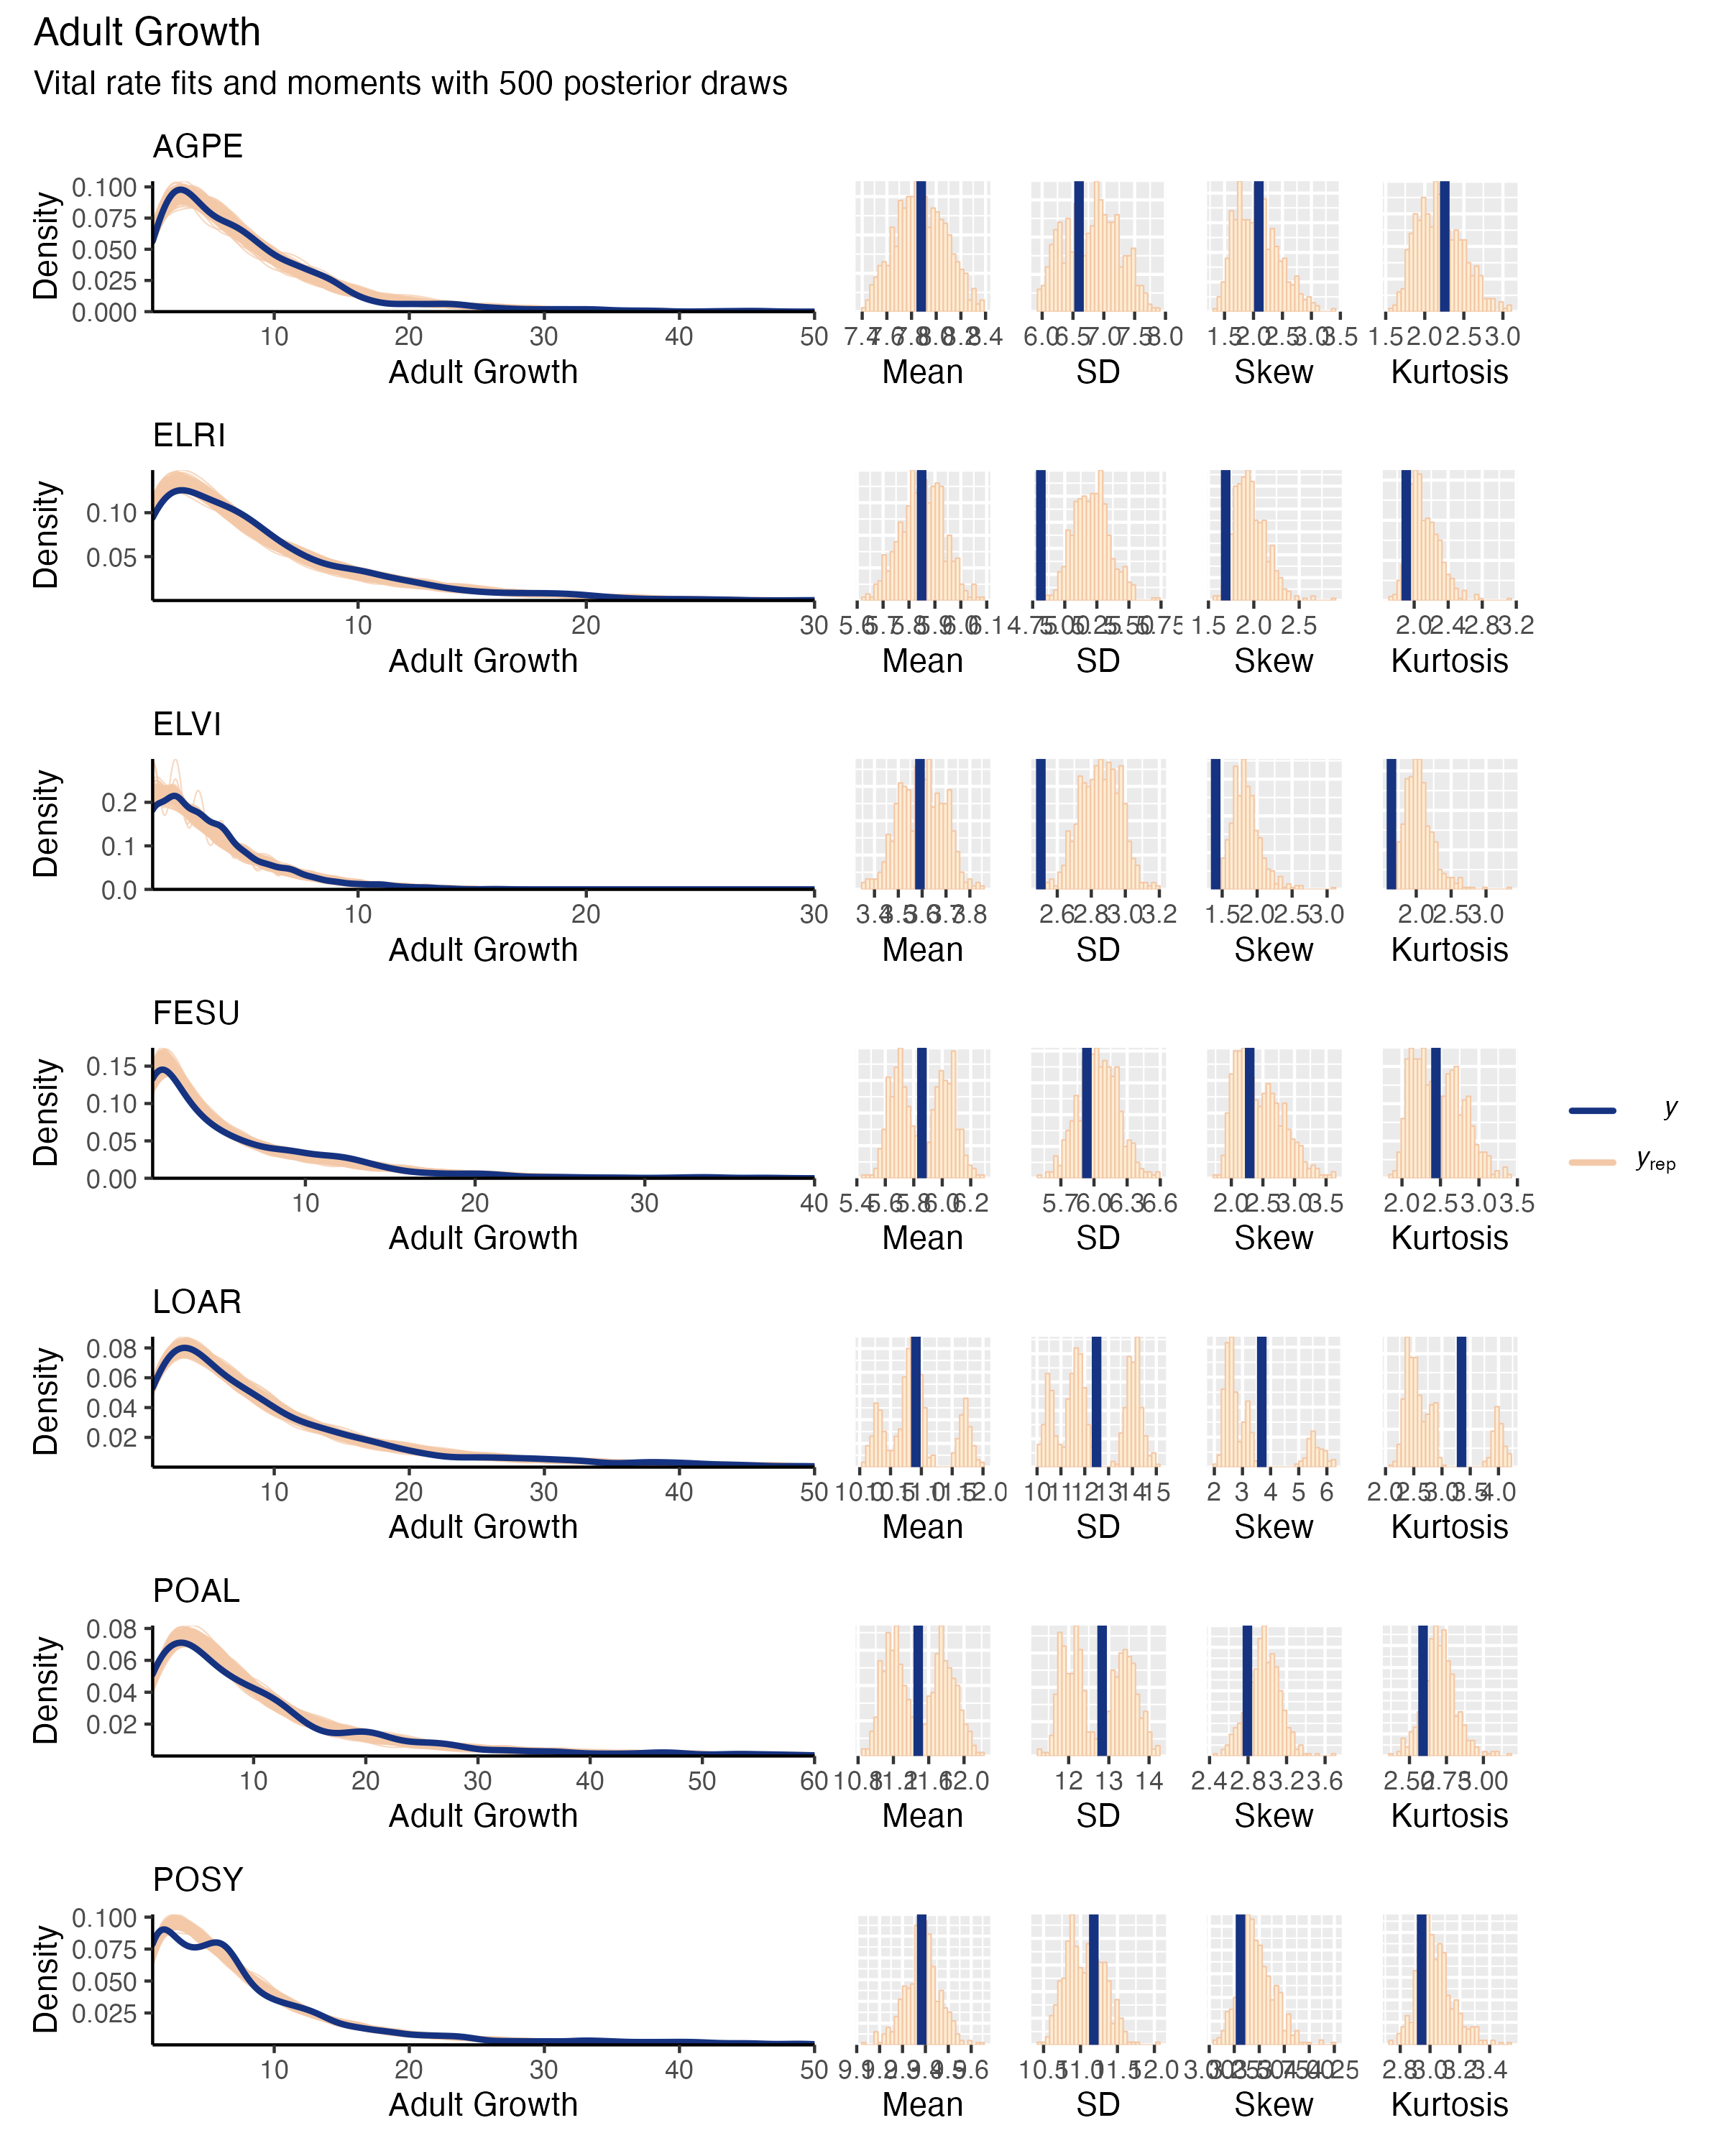
\includegraphics[width = \linewidth]{growbyspecies_densplot.png}
	\caption{Posterior predictive check for statistical model of Adult Growth. Consistency between real data and simulated values indicates that fitted models describe the data well. Lines show density distributions of observed data (blue line) compared to data simulated from fitted models (tan lines) generated from 500 draws from posterior distributions of model parameters along with the distribution's moments.}
\end{figure}

\begin{figure}[H]
	\centering
	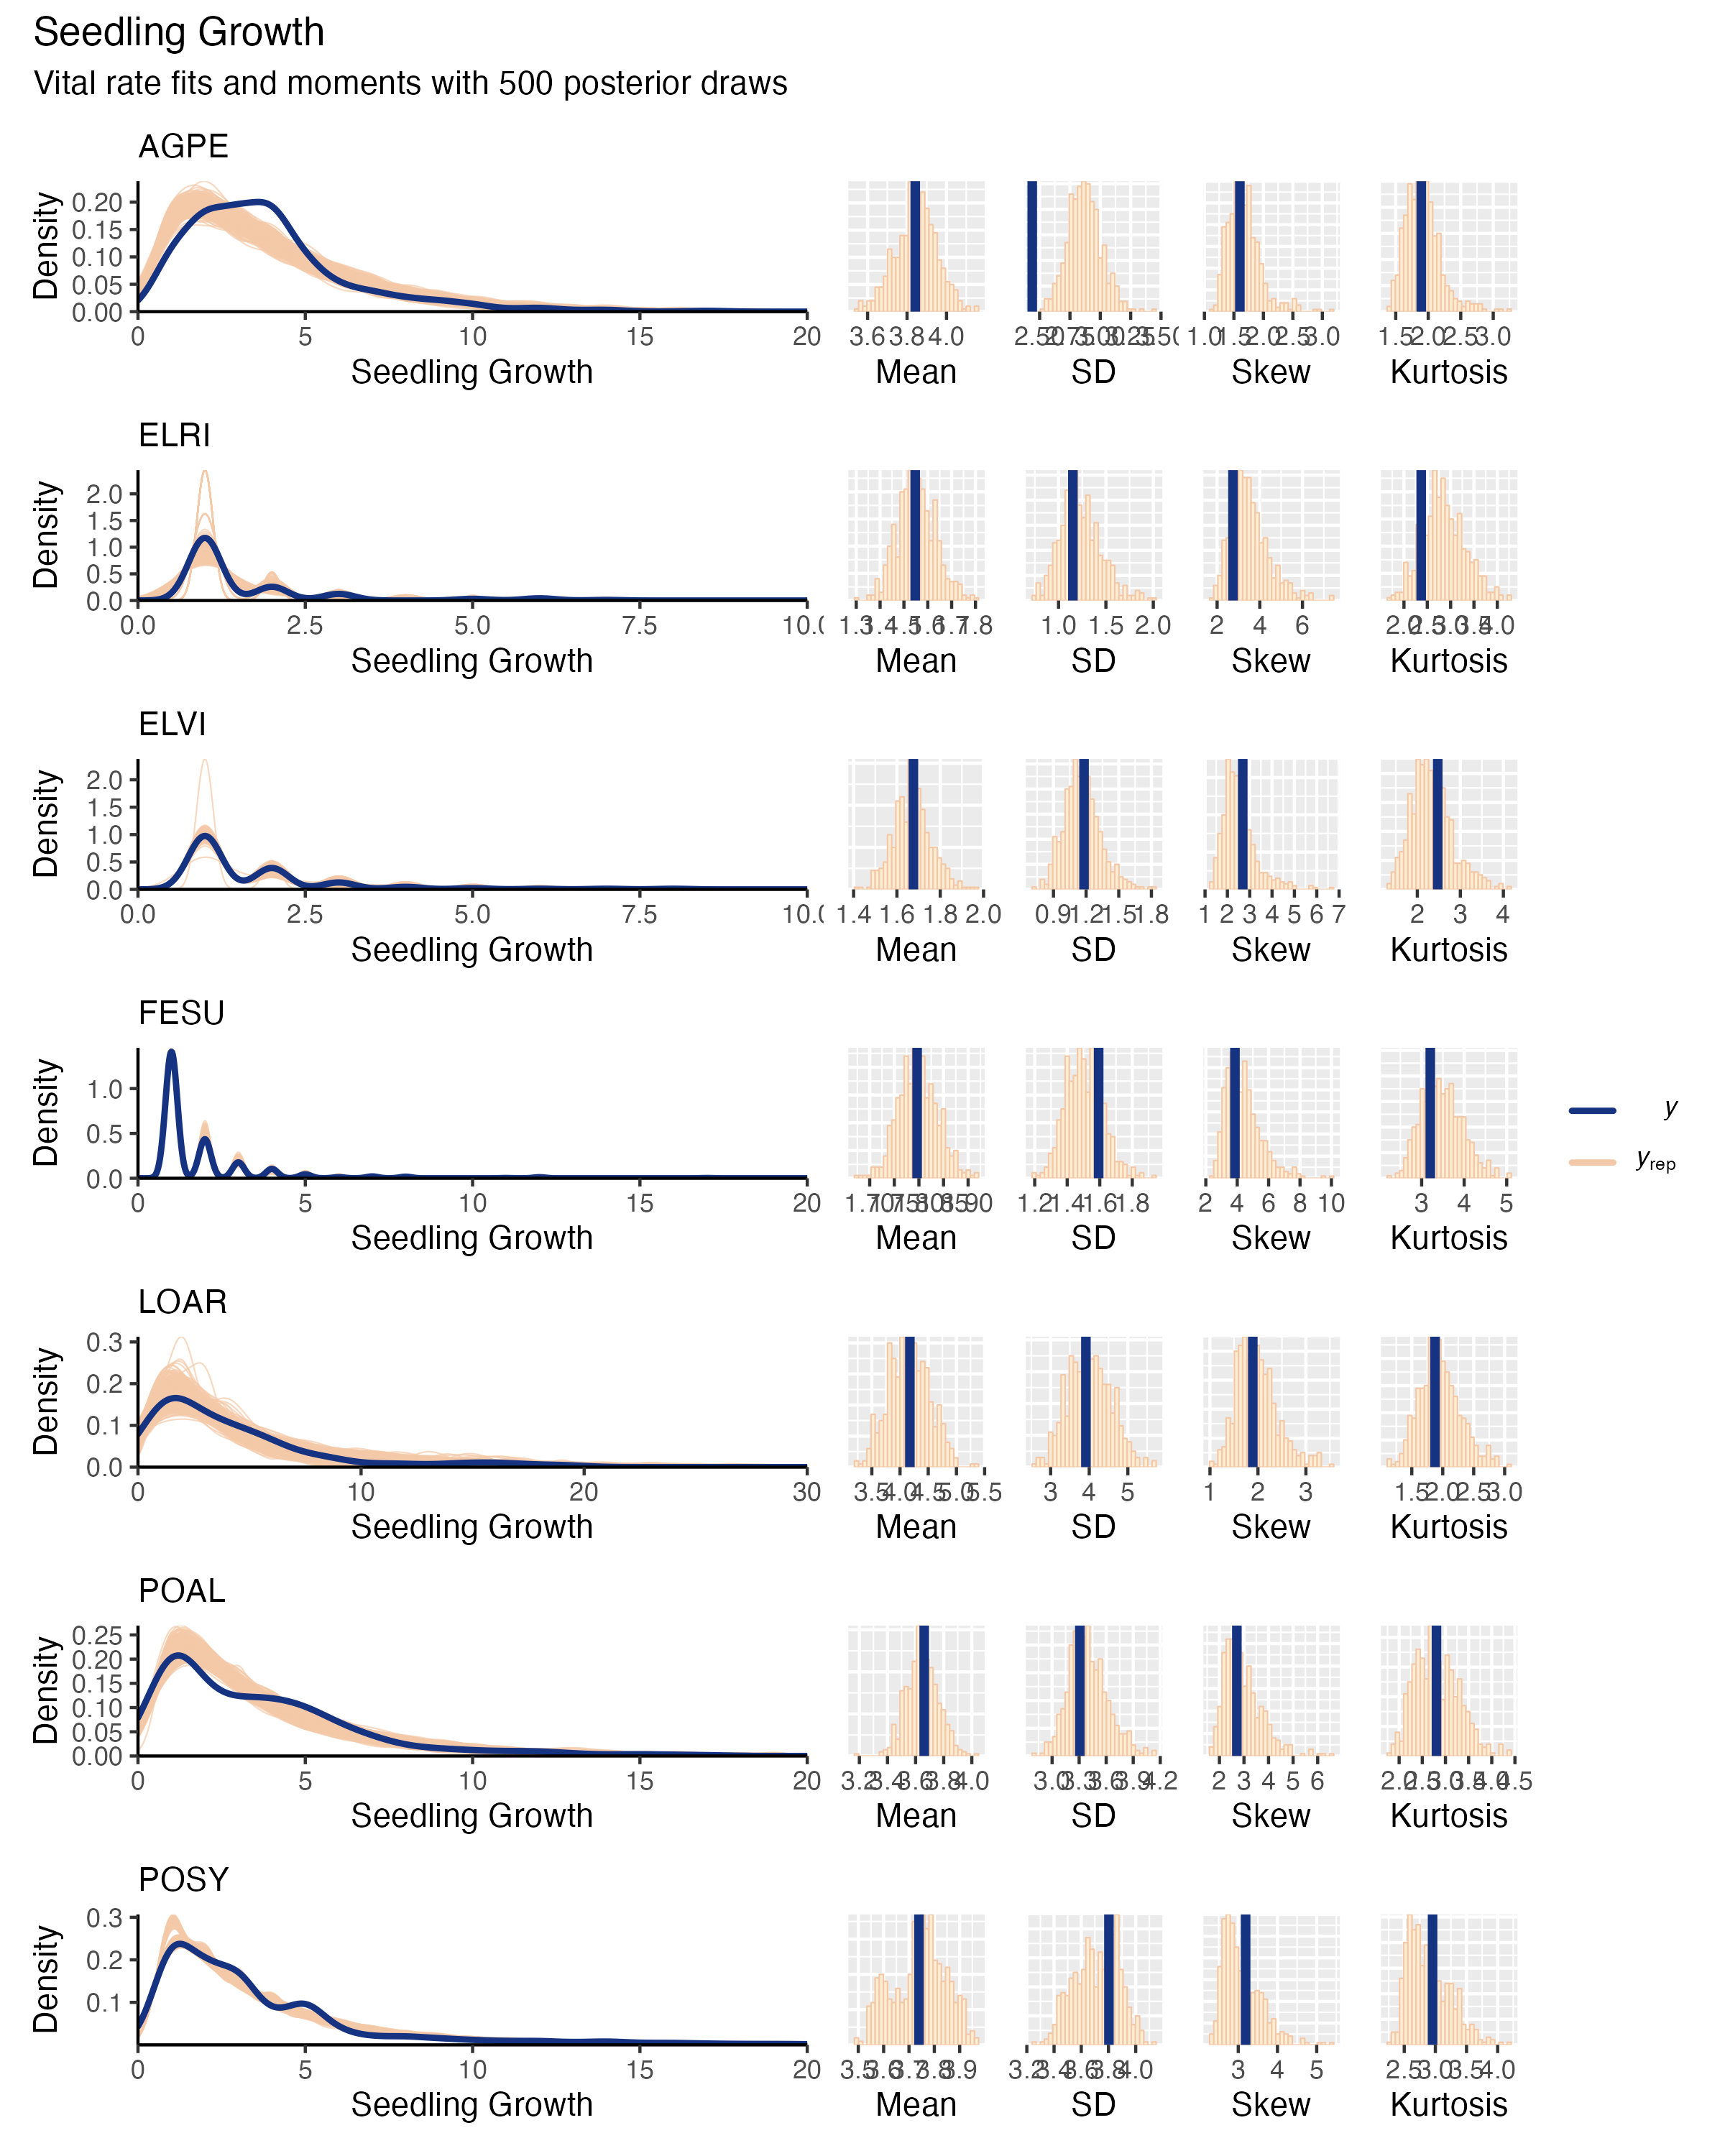
\includegraphics[width = \linewidth]{seedgrowbyspecies_densplot.png}
	\caption{Posterior predictive check for statistical model of Seedling Growth. Consistency between real data and simulated values indicates that fitted models describe the data well. Lines show density distributions of observed data (blue line) compared to data simulated from fitted models (tan lines) generated from 500 draws from posterior distributions of model parameters along with the distribution's moments.}
\end{figure}


\begin{figure}[H]
	\centering
	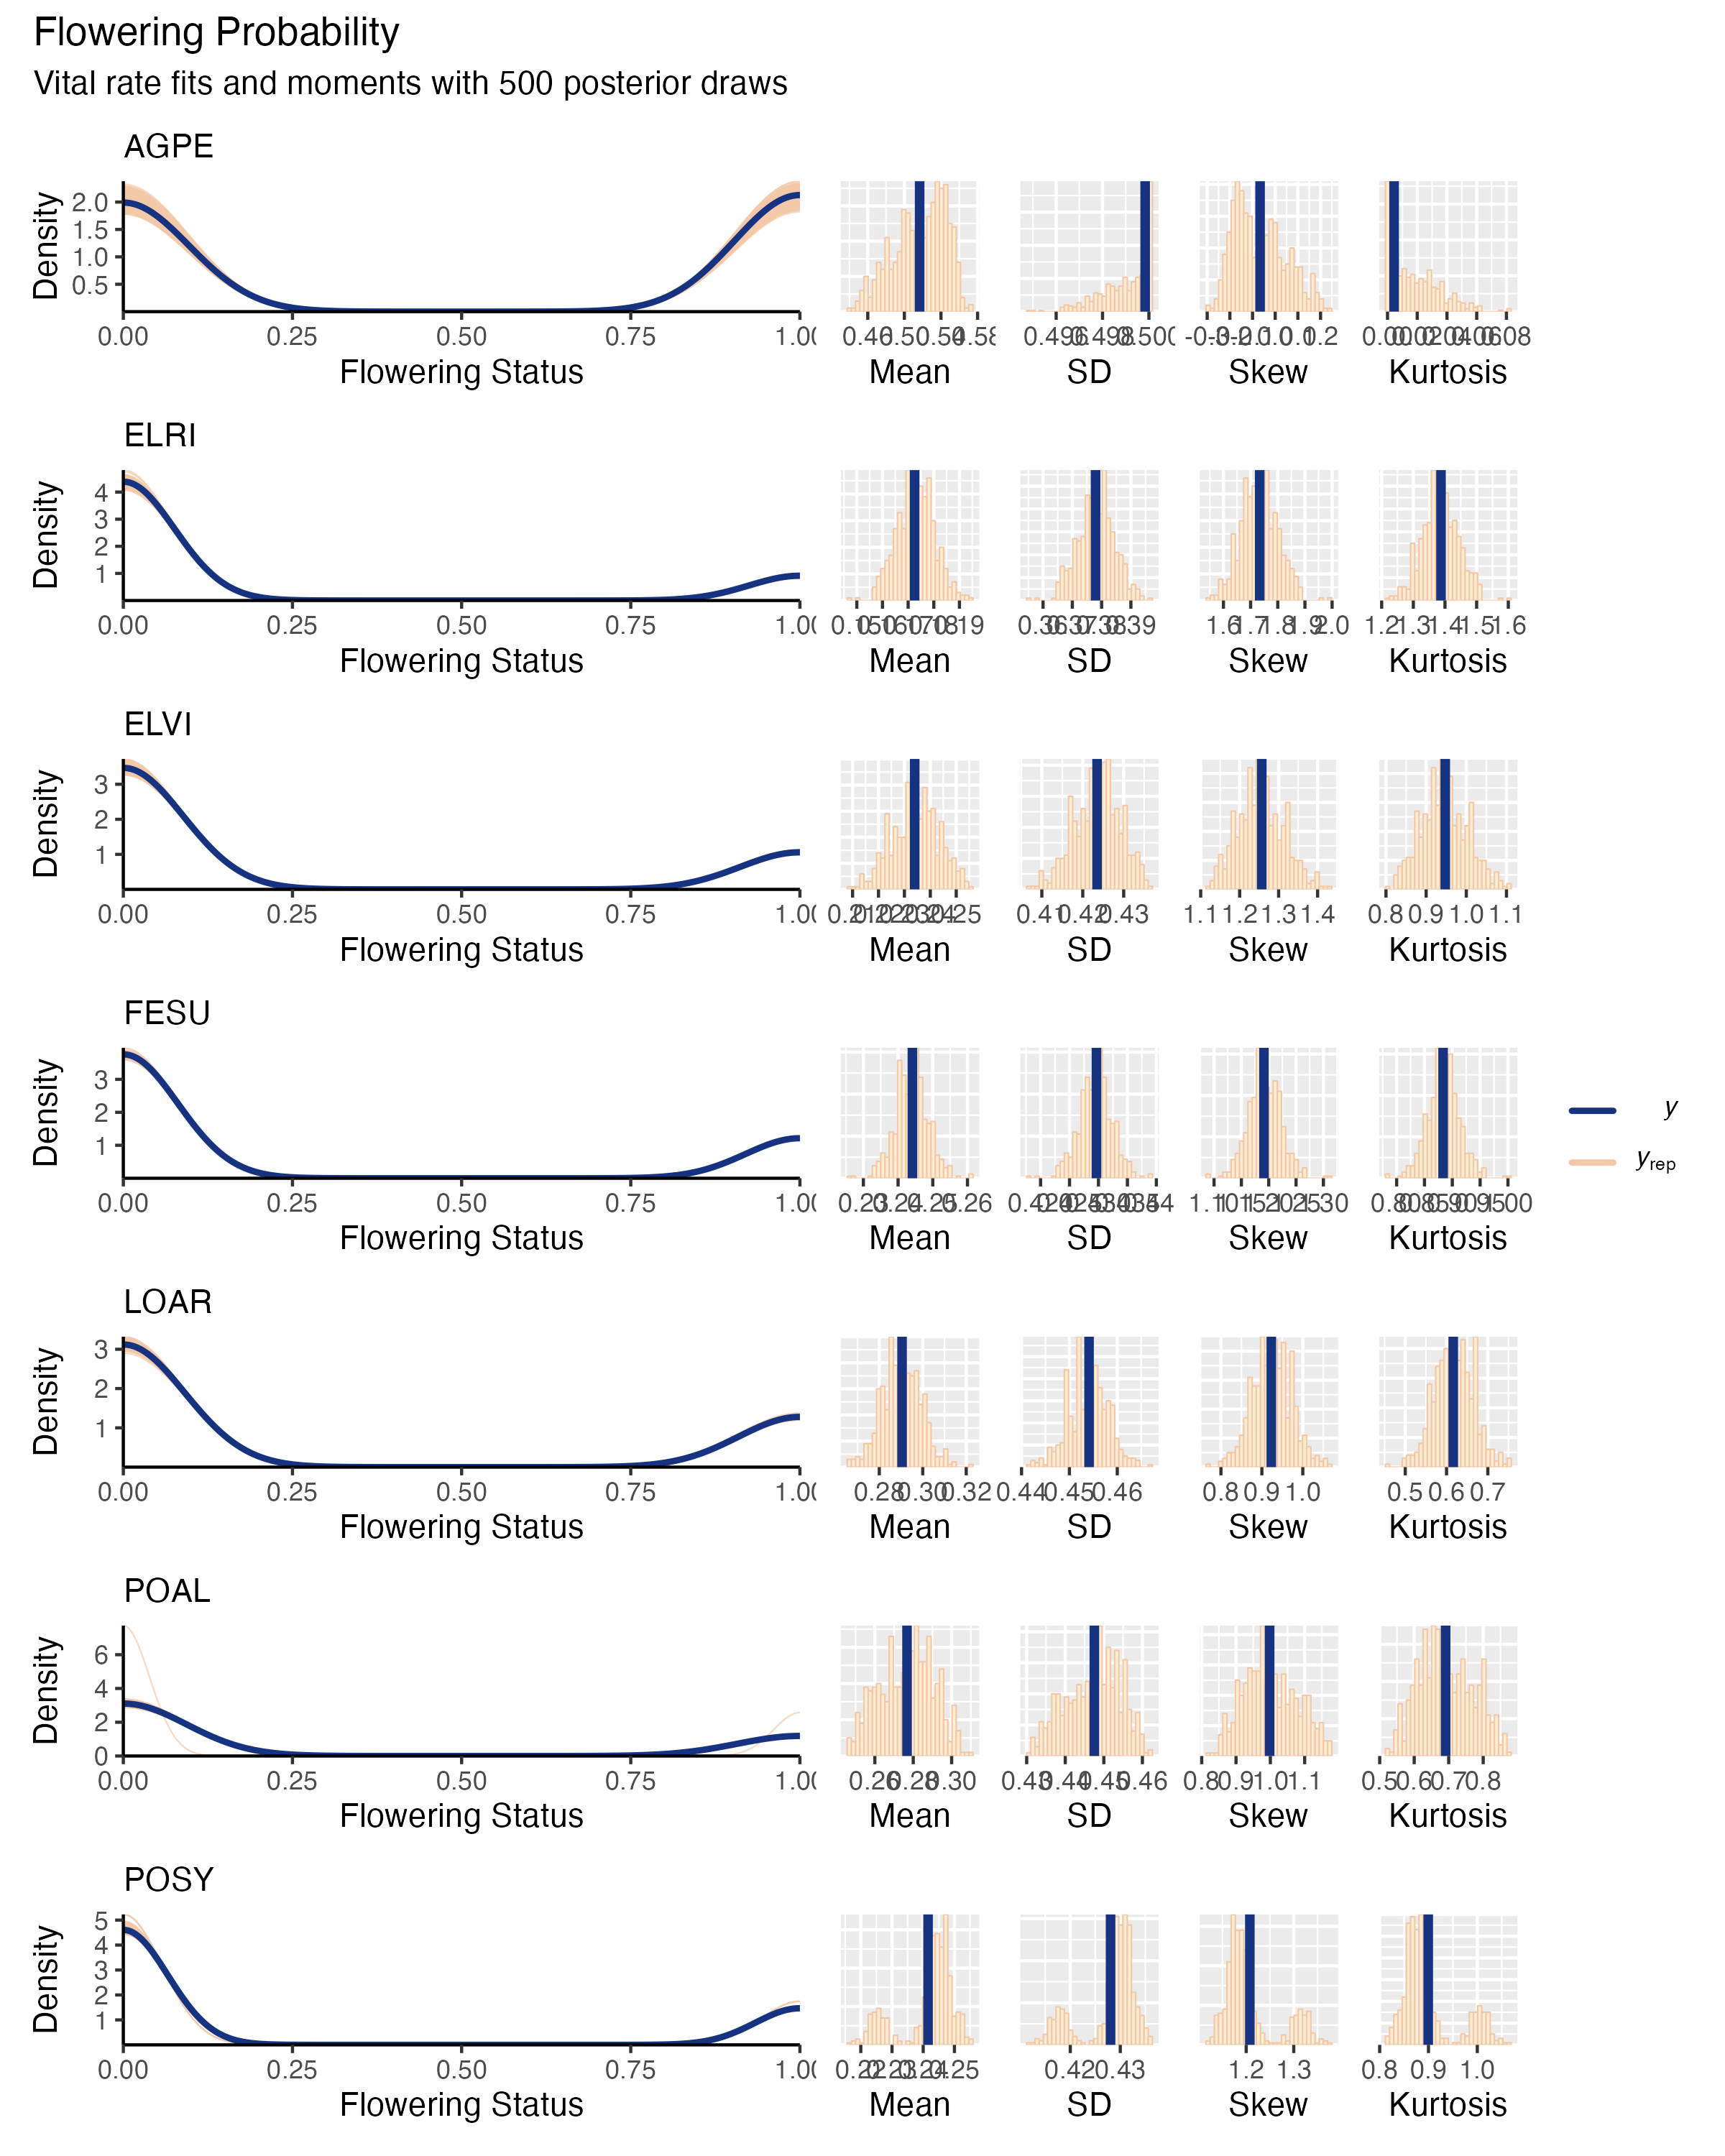
\includegraphics[width = \linewidth]{flwbyspecies_densplot.png}
	\caption{Posterior predictive check for statistical model of Flowering Probability. Consistency between real data and simulated values indicates that fitted models describe the data well. Lines show density distributions of observed data (blue line) compared to data simulated from fitted models (tan lines) generated from 500 draws from posterior distributions of model parameters along with the distribution's moments.}
\end{figure}

\begin{figure}[H]
	\centering
	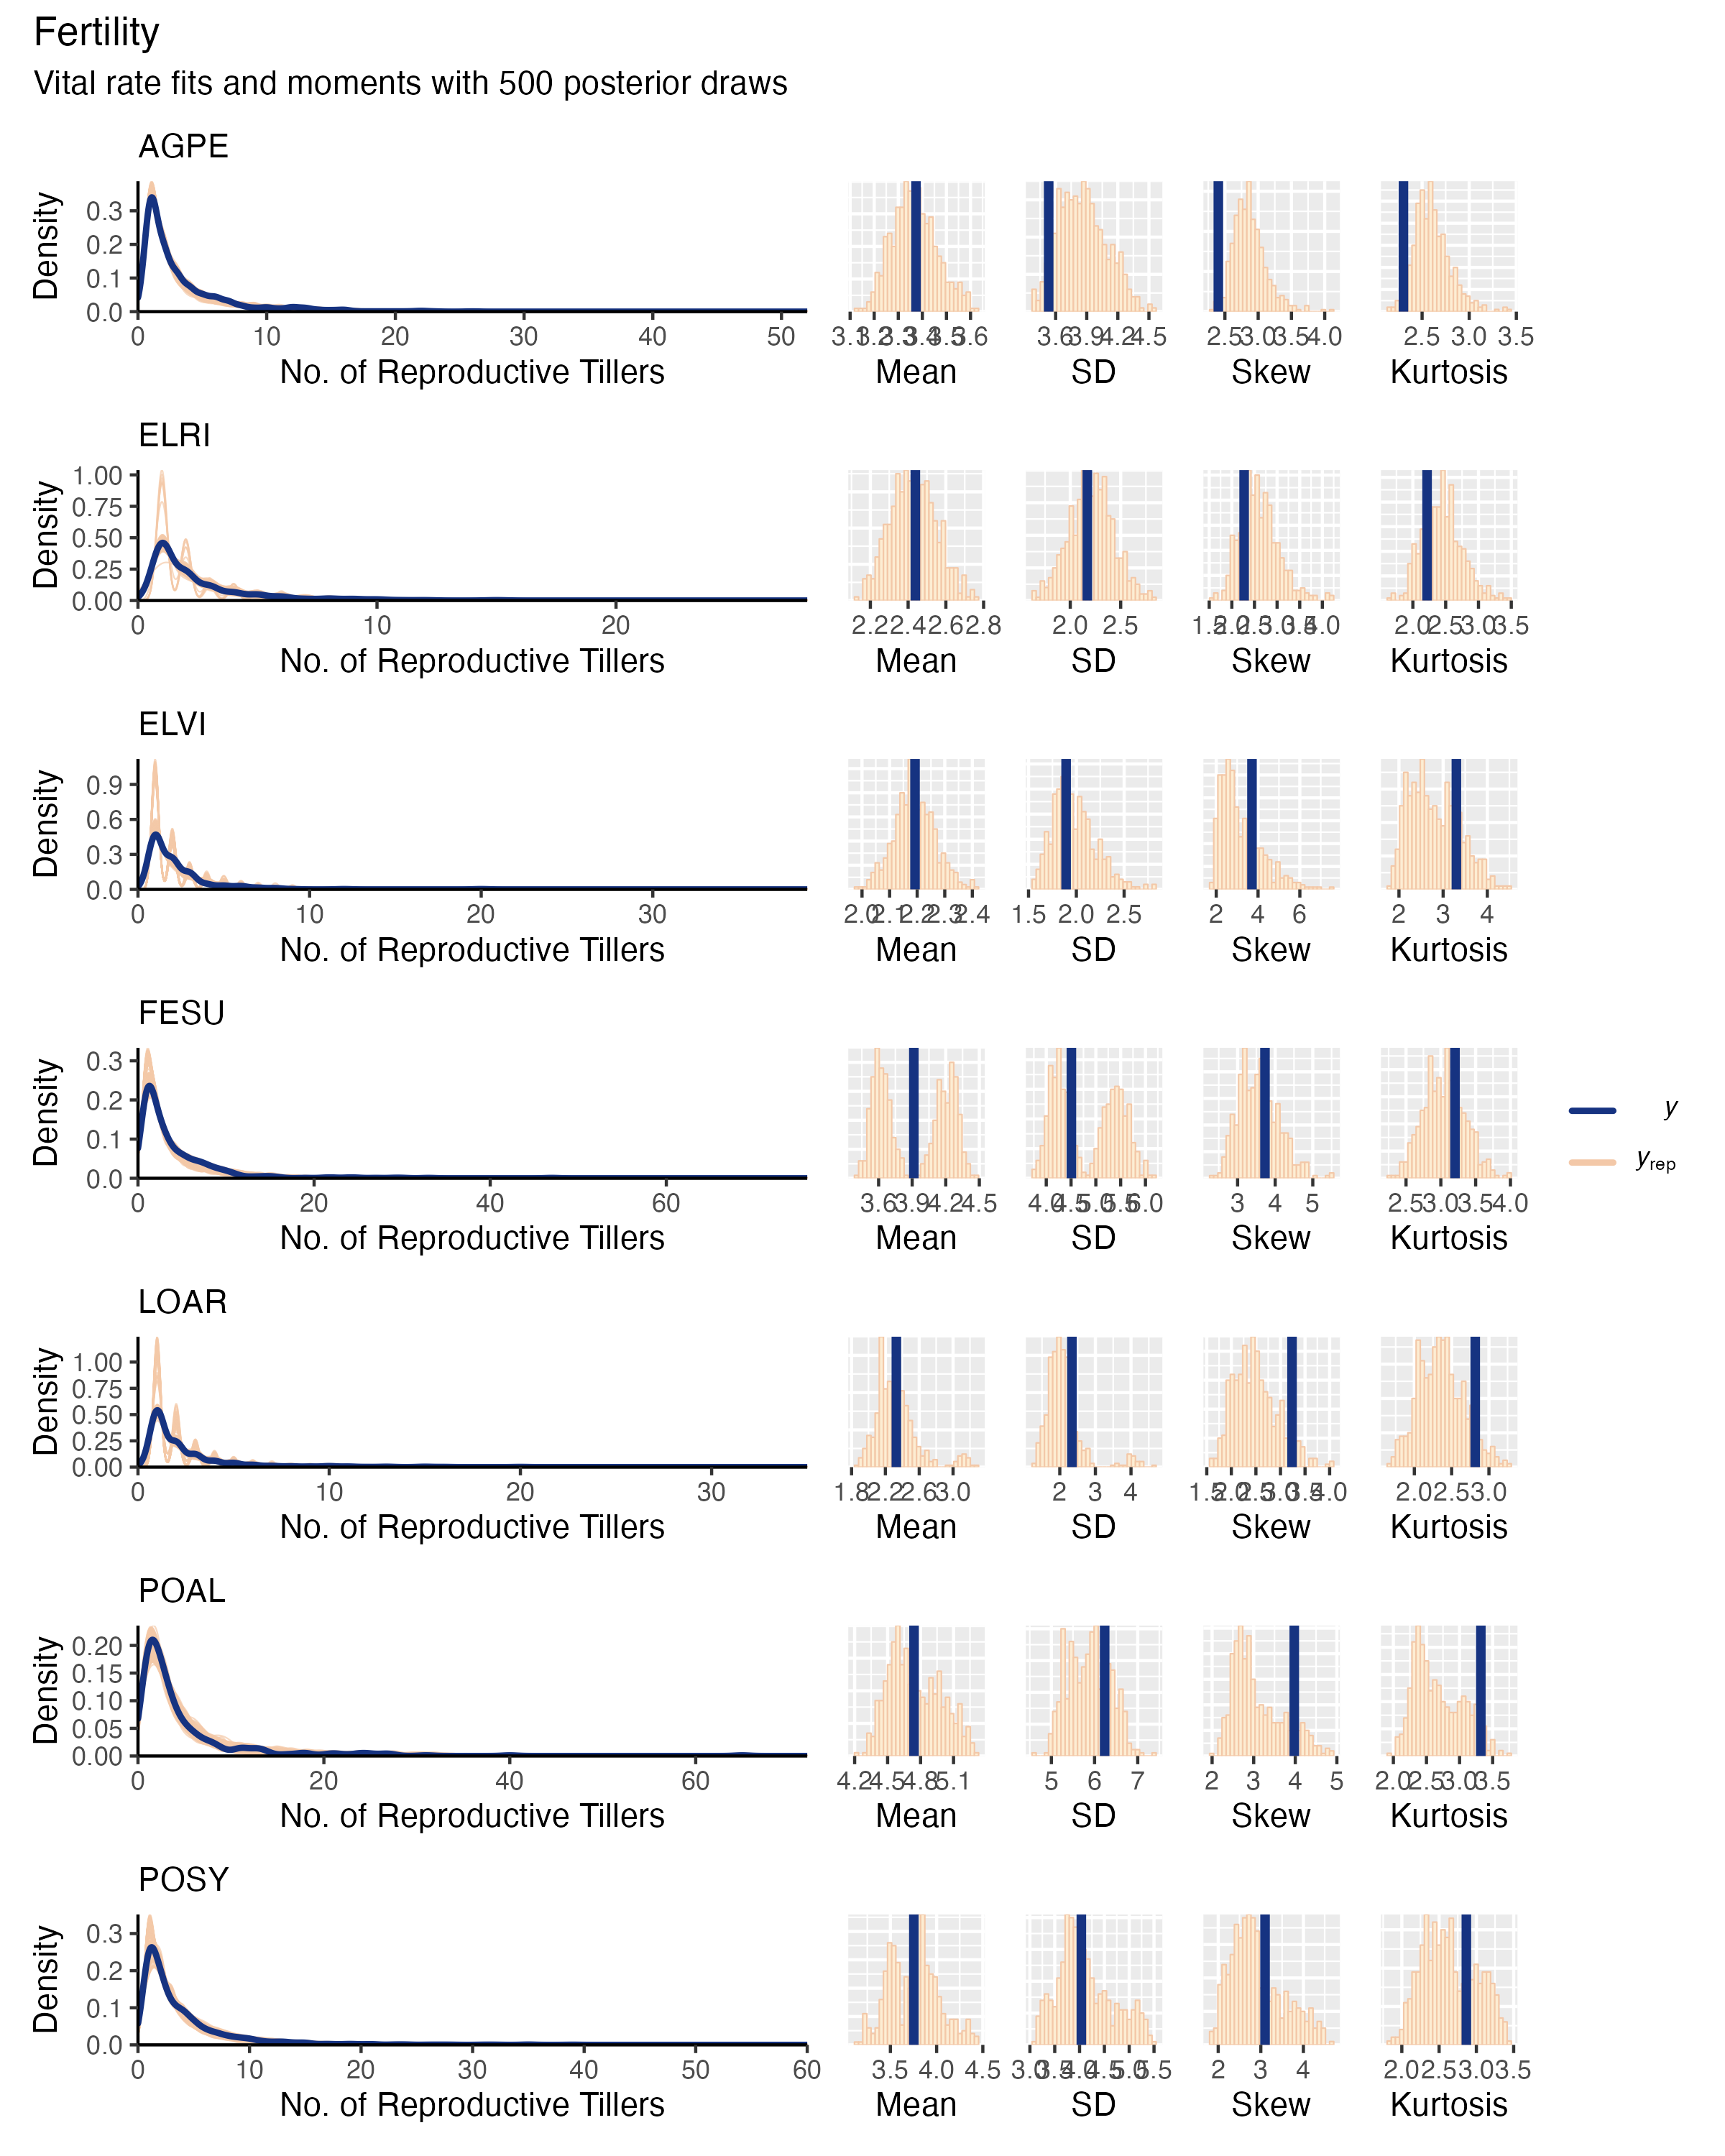
\includegraphics[width = \linewidth]{fertbyspecies_densplot.png}
	\caption{Posterior predictive check for statistical model of Flowering Tiller production. Consistency between real data and simulated values indicates that fitted models describe the data well. Lines show density distributions of observed data (blue line) compared to data simulated from fitted models (tan lines) generated from 500 draws from posterior distributions of model parameters along with the distribution's moments.}
\end{figure}


\begin{figure}[H]
	\centering
	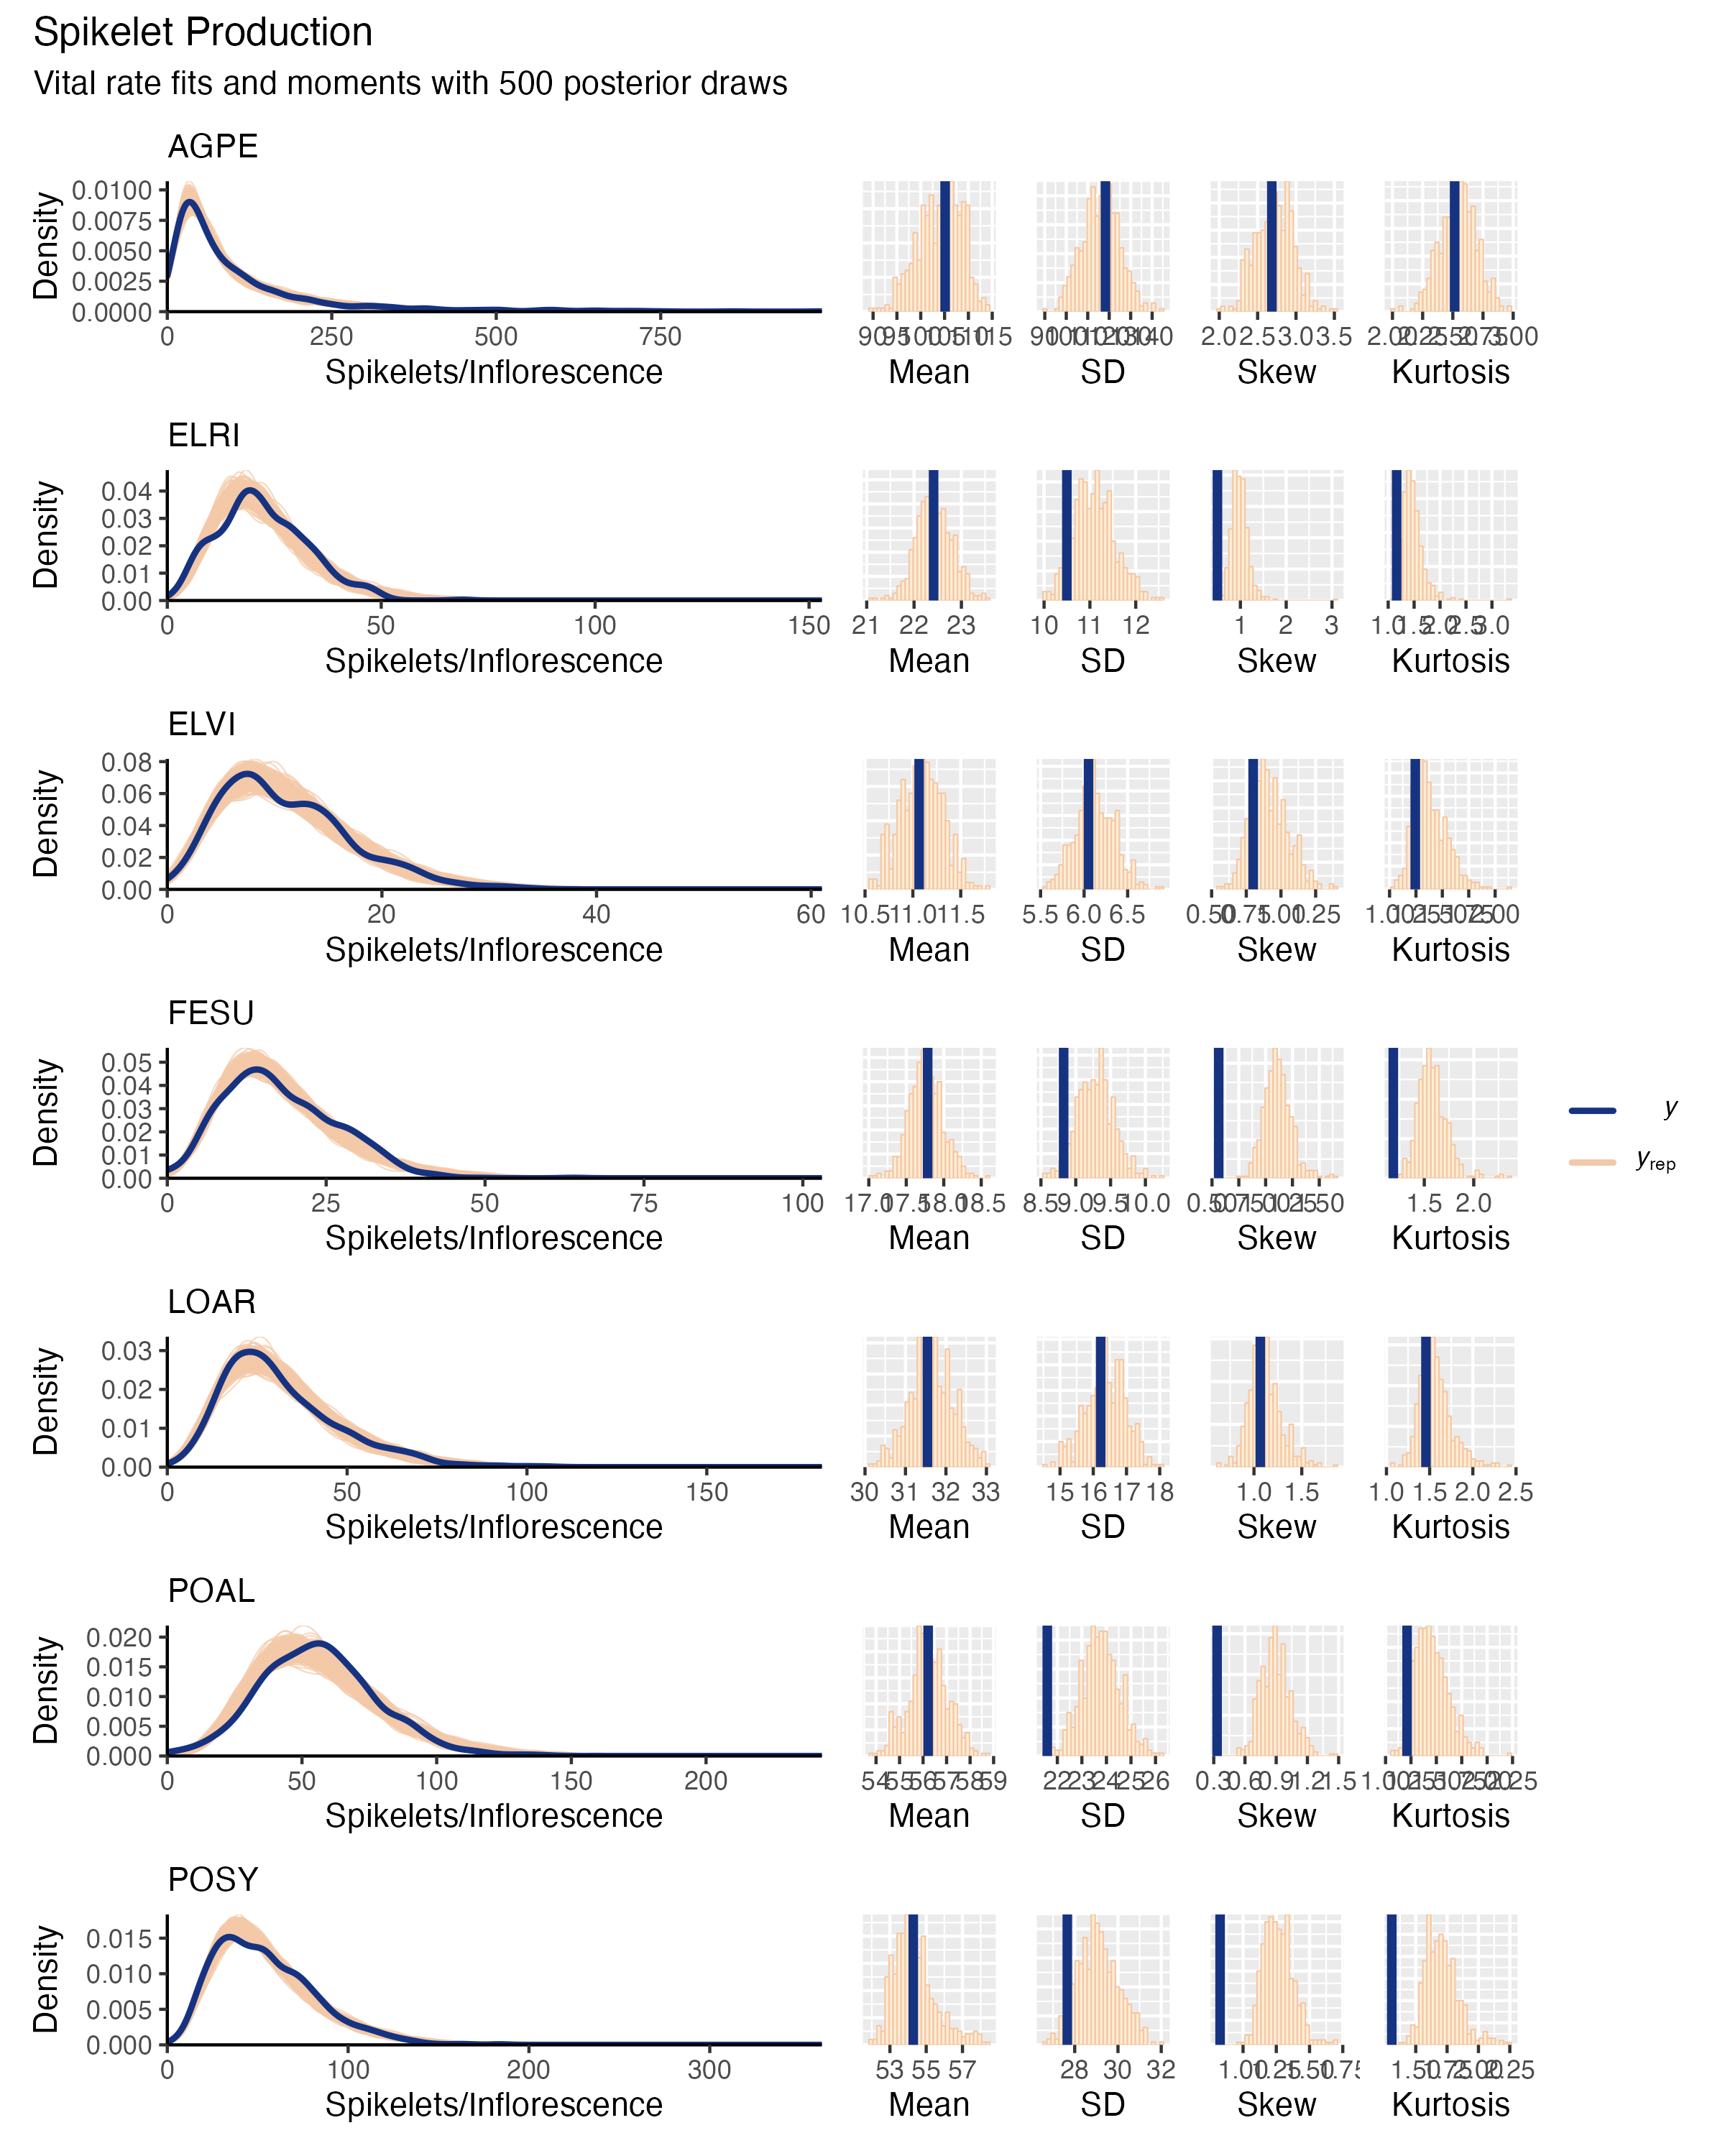
\includegraphics[width = \linewidth]{spikebyspecies_densplot.png}
	\caption{Posterior predictive check for statistical model of Spikelets/Inflorescence. Consistency between real data and simulated values indicates that fitted models describe the data well. Lines show density distributions of observed data (blue line) compared to data simulated from fitted models (tan lines) generated from 500 draws from posterior distributions of model parameters along with the distribution's moments.}
\end{figure}

\begin{figure}[H]
	\centering
	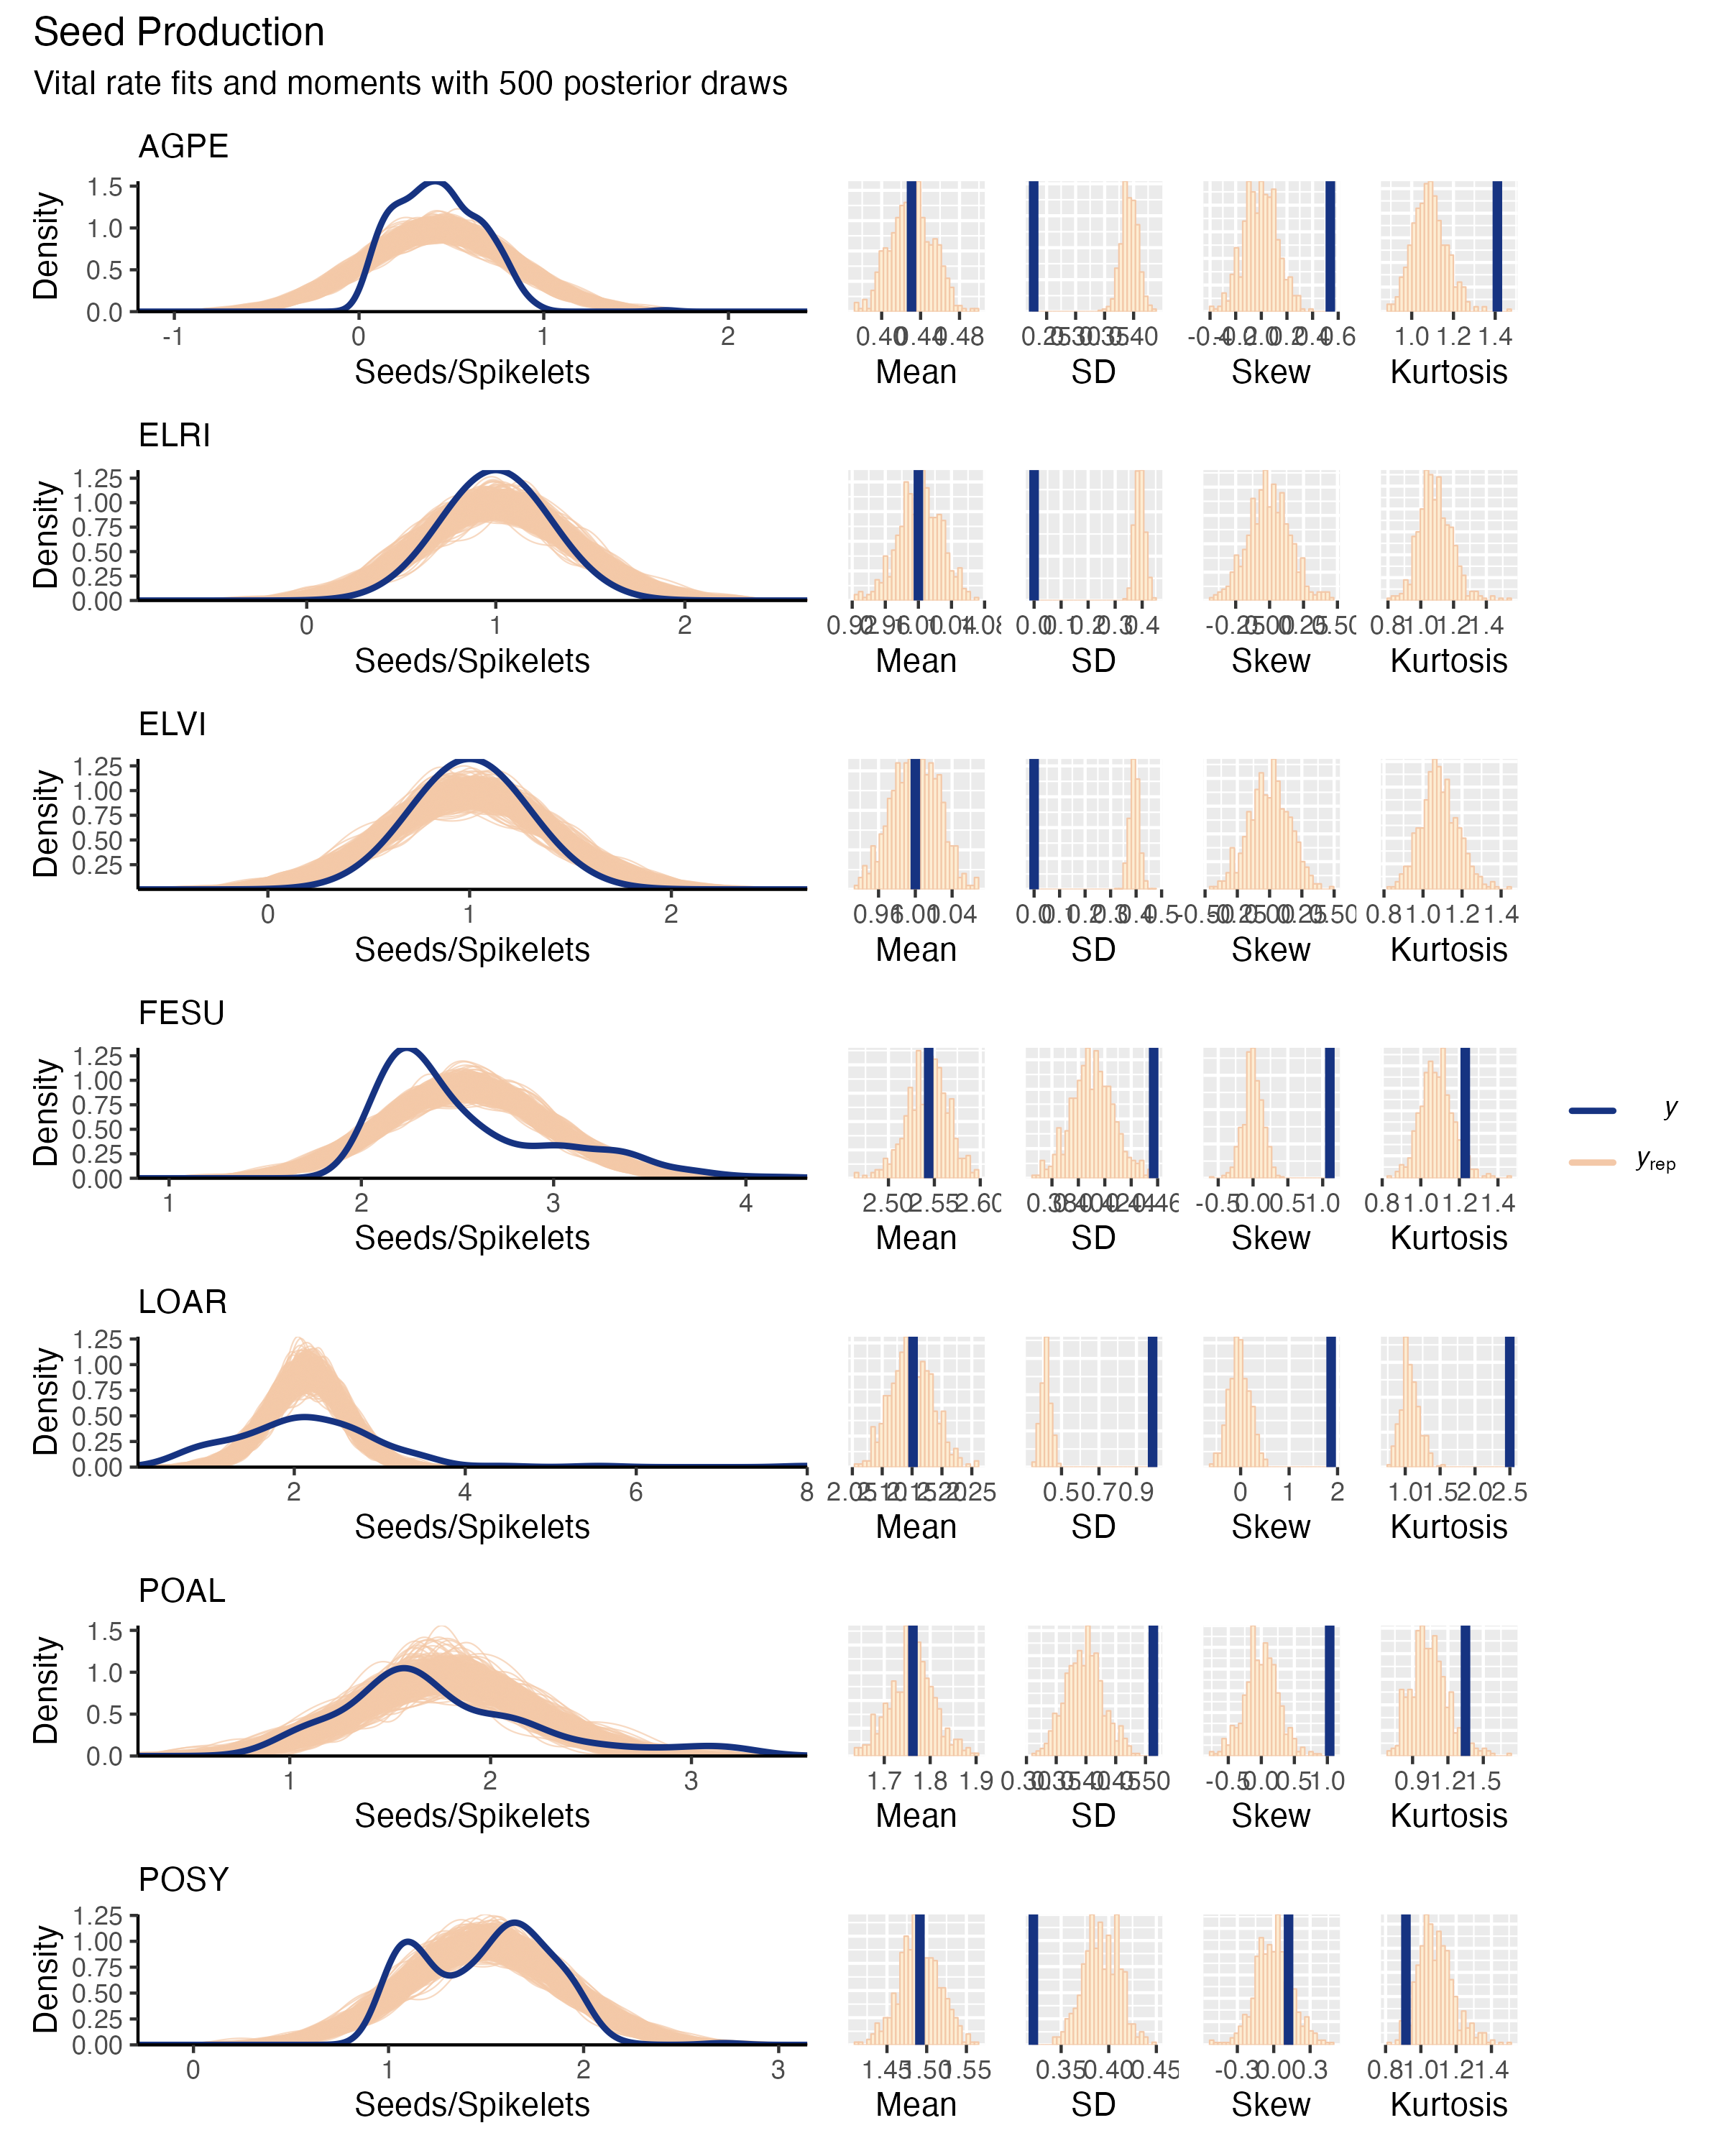
\includegraphics[width = \linewidth]{seedmeanbyspecies_densplot.png}
	\caption{Posterior predictive check for statistical model of Mean Seeds/Spikelet. Consistency between real data and simulated values indicates that fitted models describe the data well. Lines show density distributions of observed data (blue line) compared to data simulated from fitted models (tan lines) generated from 500 draws from posterior distributions of model parameters along with the distribution's moments.}
\end{figure}

\begin{figure}[H]
	\centering
	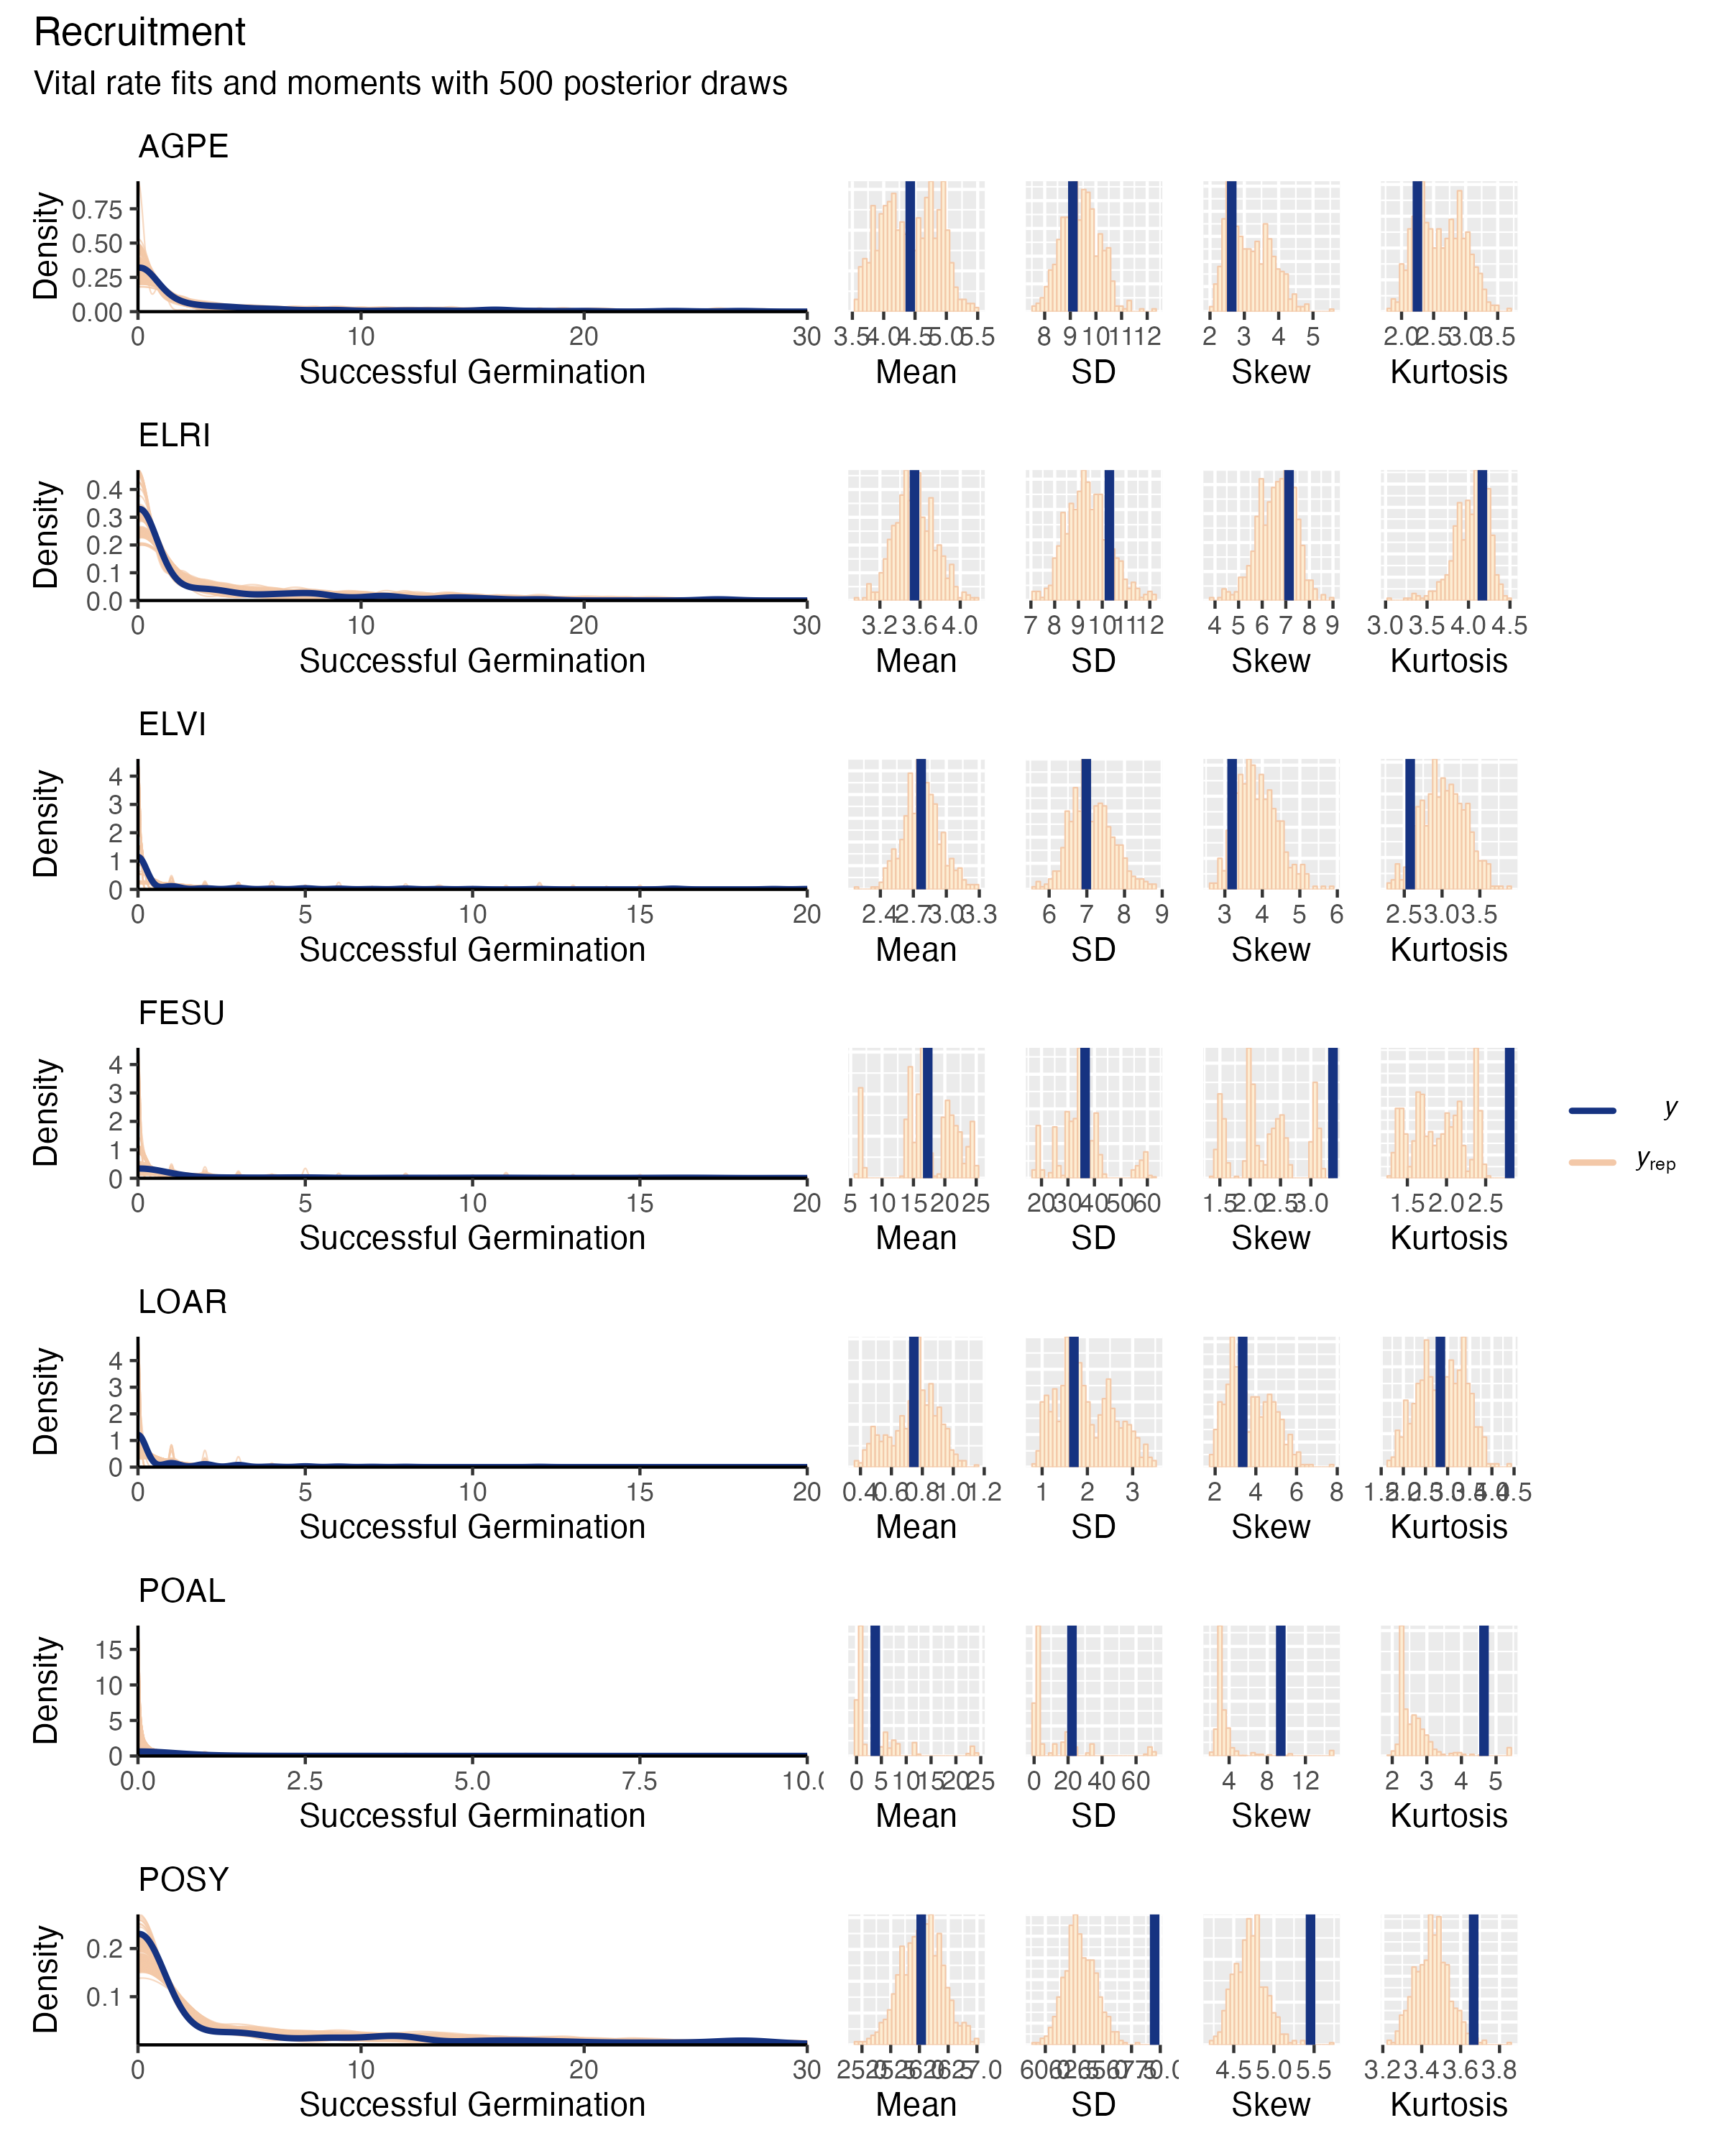
\includegraphics[width = \linewidth]{stosbyspecies_densplot.png}
	\caption{Posterior predictive check for statistical model of Recruitment. Consistency between real data and simulated values indicates that fitted models describe the data well. Lines show density distributions of observed data (blue line) compared to data simulated from fitted models (tan lines) generated from 500 draws from posterior distributions of model parameters along with the distribution's moments.}
\end{figure}


\begin{figure}[H]
	\centering
	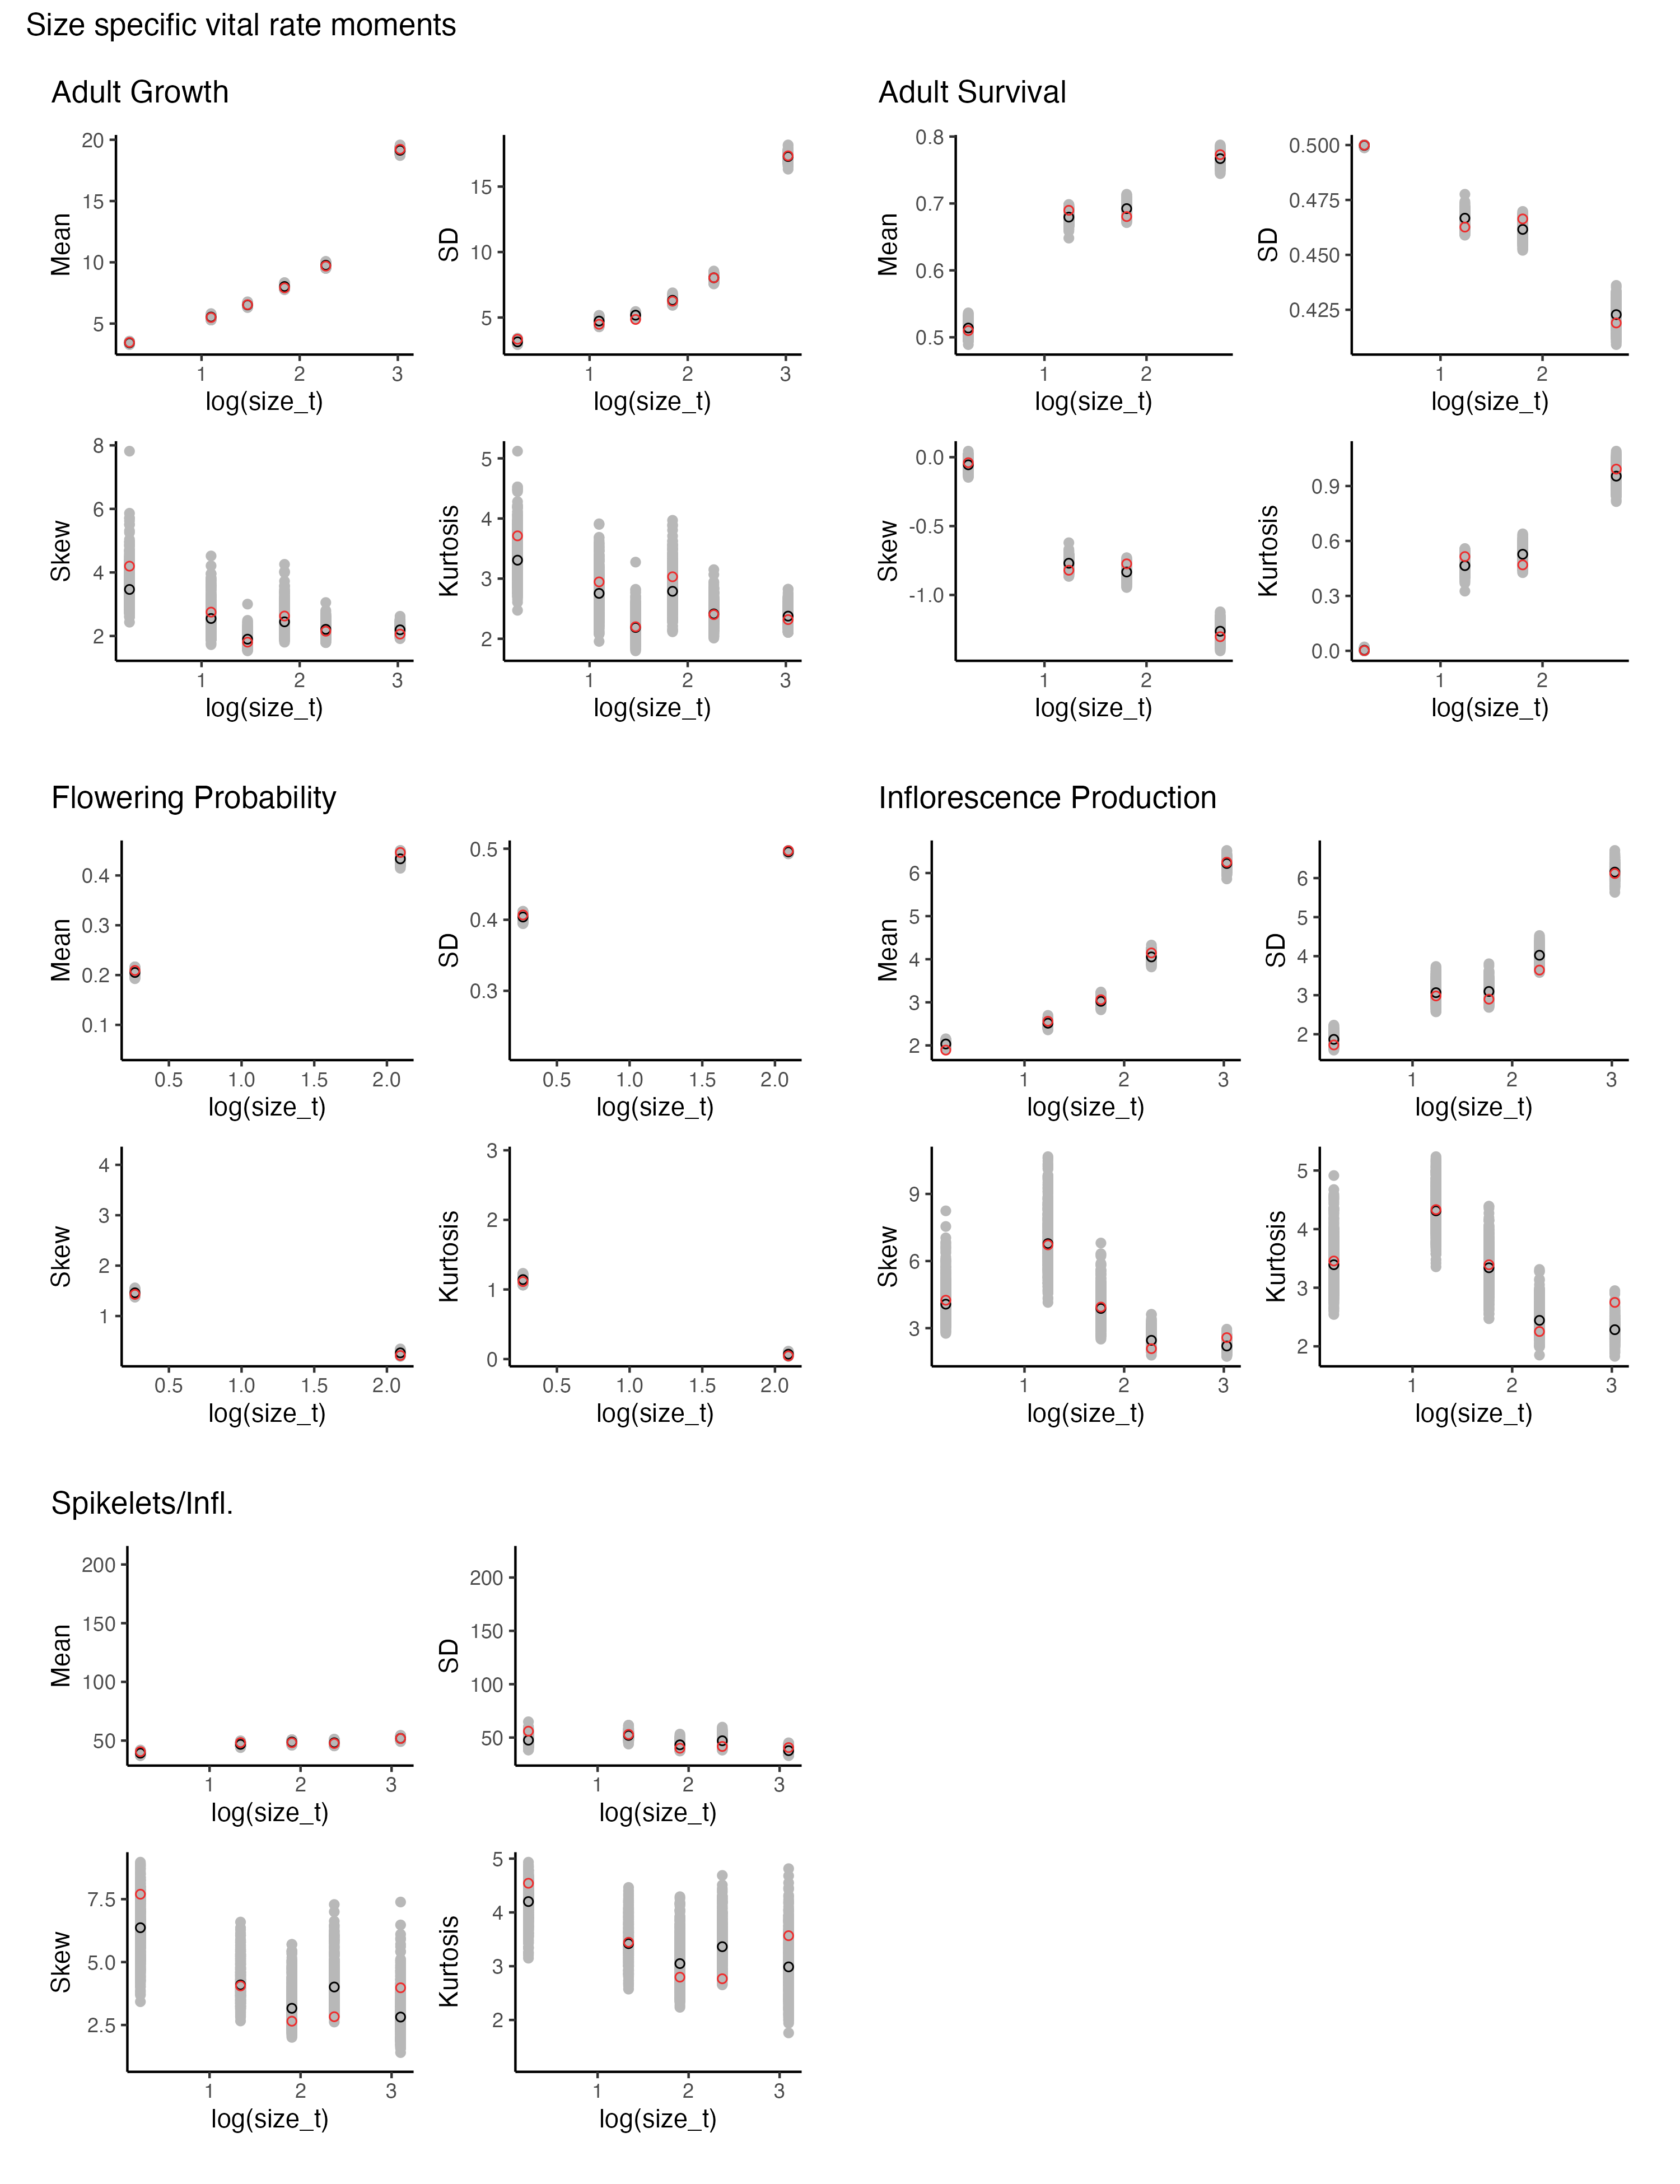
\includegraphics[width = \linewidth]{size_ppc_plot.png}
	\caption{Consistency between real data and fitted values across sizes indicates that the vital rate models are accurately capturing size dependence. Graphs of posterior predictive check for mean and higher moments of the vital rate models across size. Points show the value of statistical moments binned across size for the observed data (red circles) compared to the simulated datasets (grey circles) and the median of the simulated values (black circles) generated from 500 posterior draws from the fitted model. }
\end{figure}


\begin{figure}[H]
	\centering
	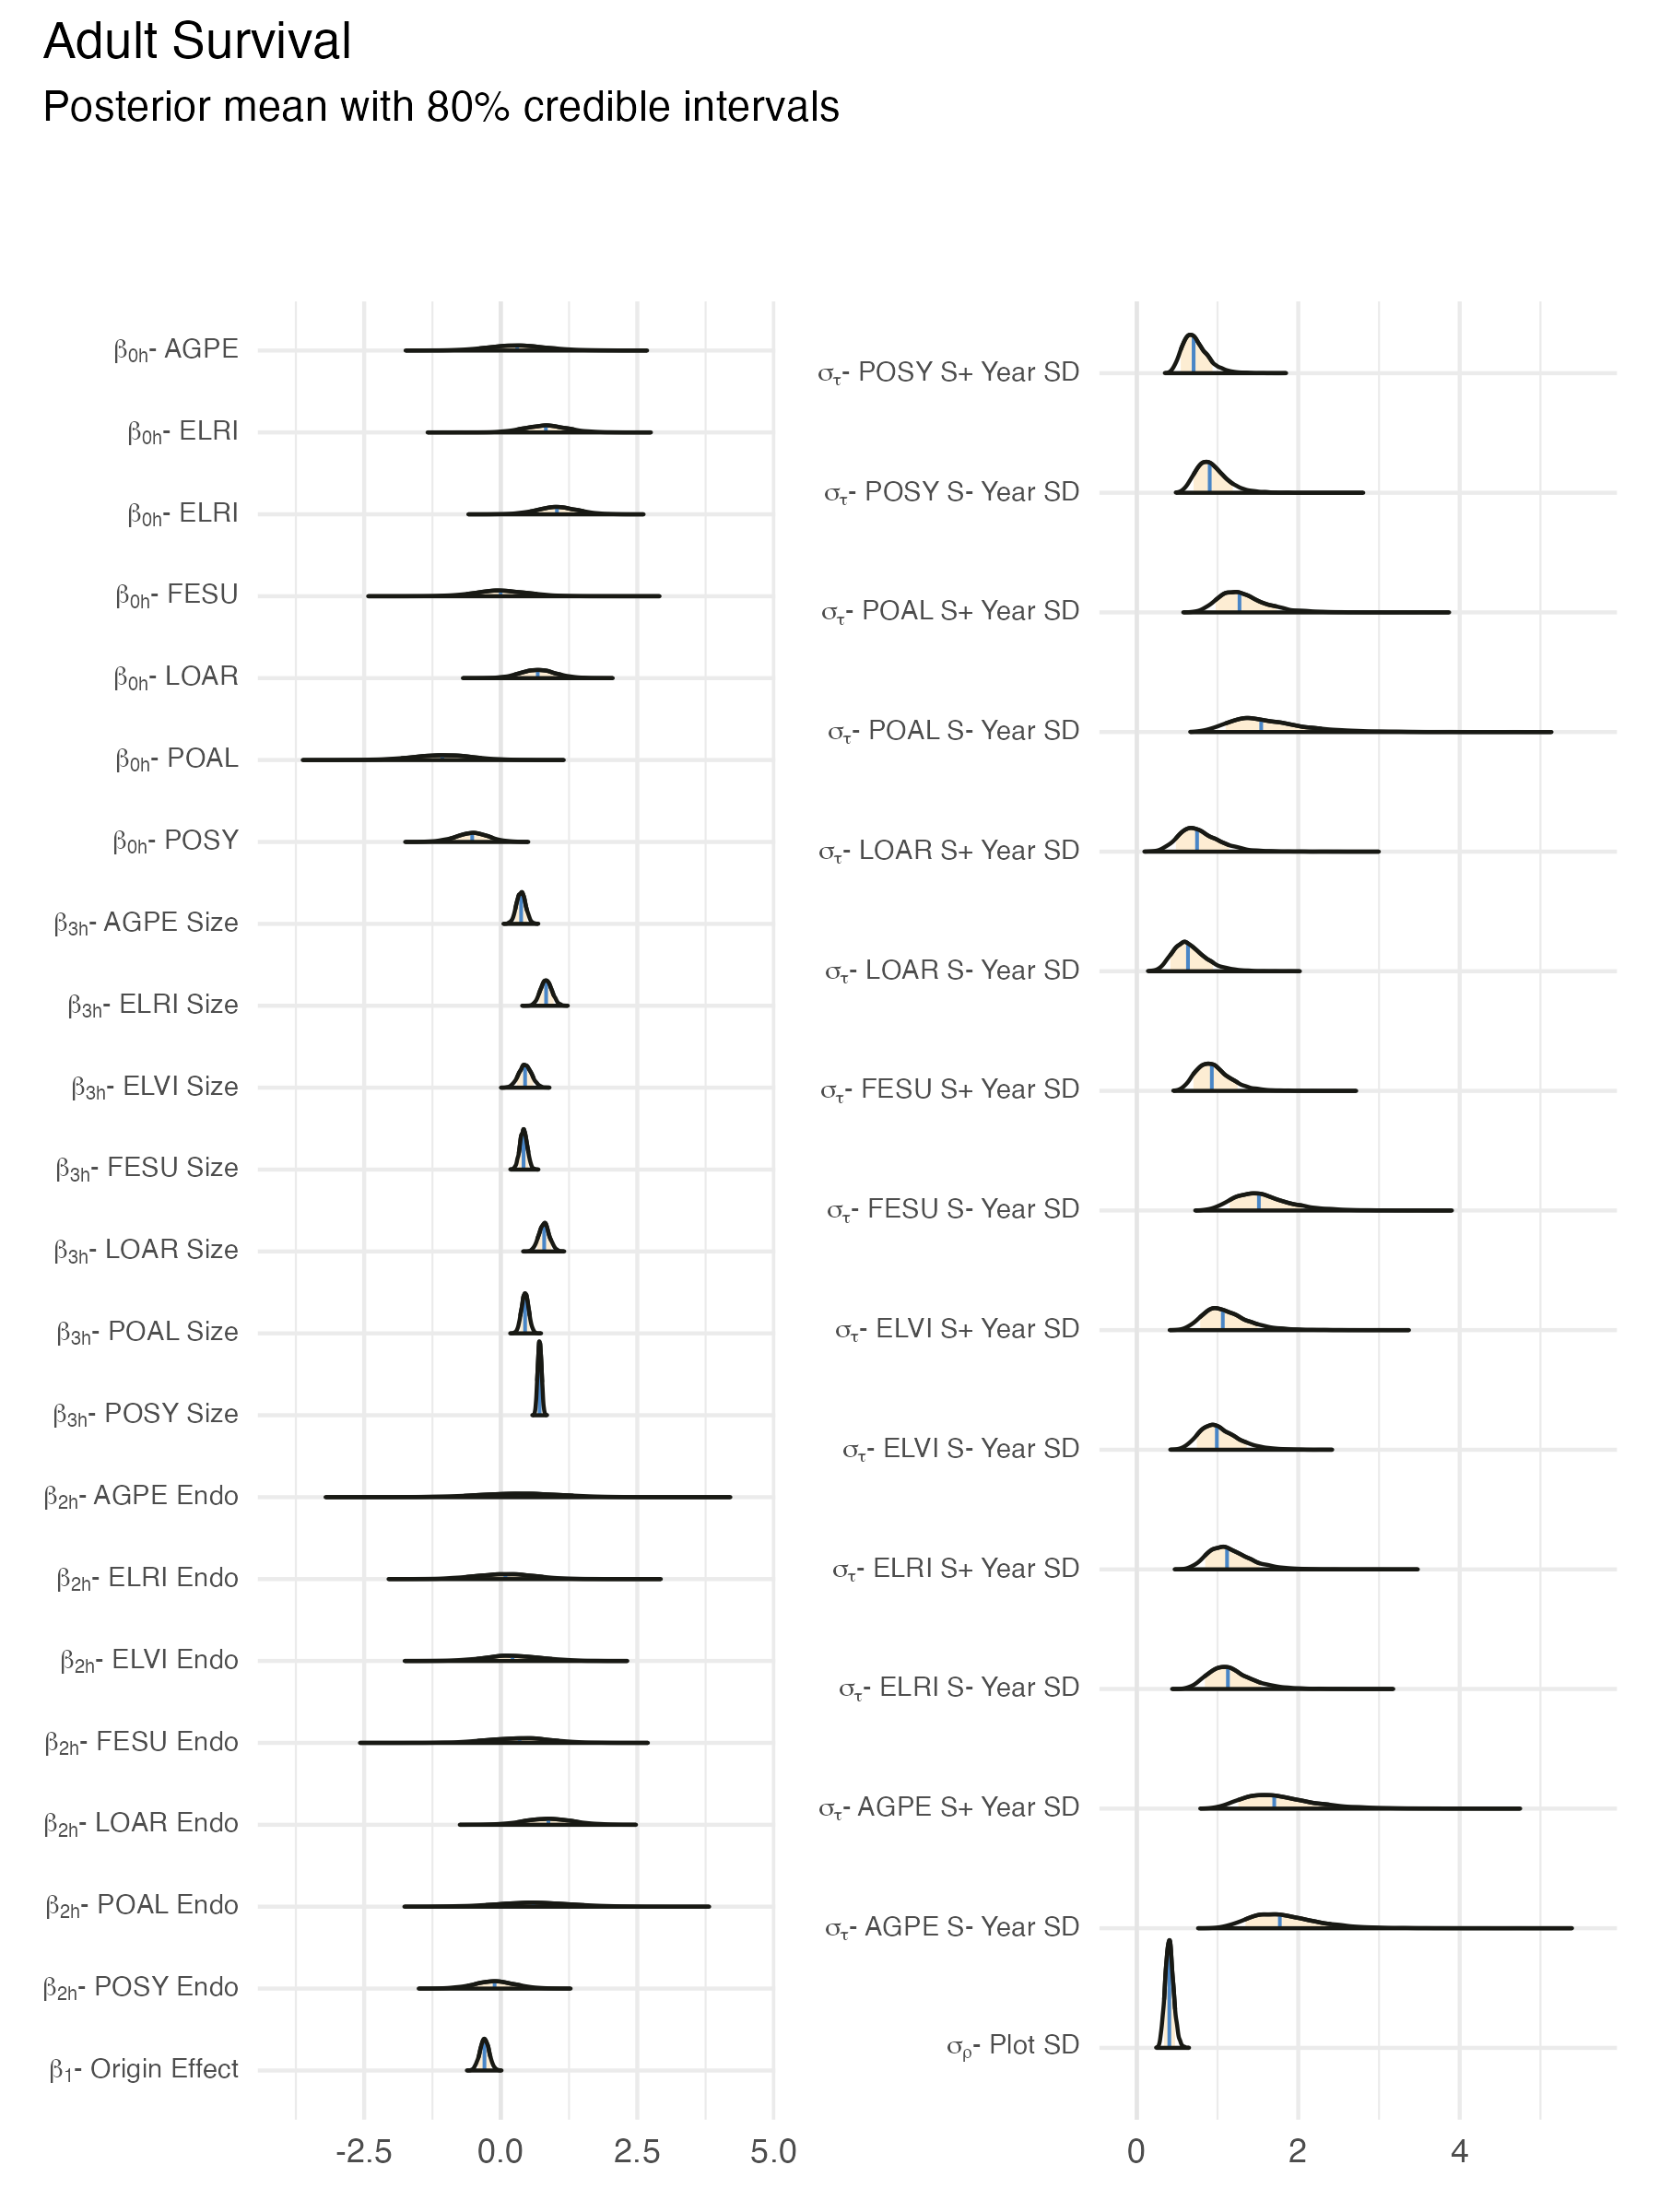
\includegraphics[width = \linewidth]{surv_posteriors_plot.png}
	\caption{Posterior distributions of the vital rate regressions for Adult Survival. Density curves show $80\%$ credible interval along with the posterior posterior mean.}
\end{figure}

\begin{figure}[H]
	\centering
	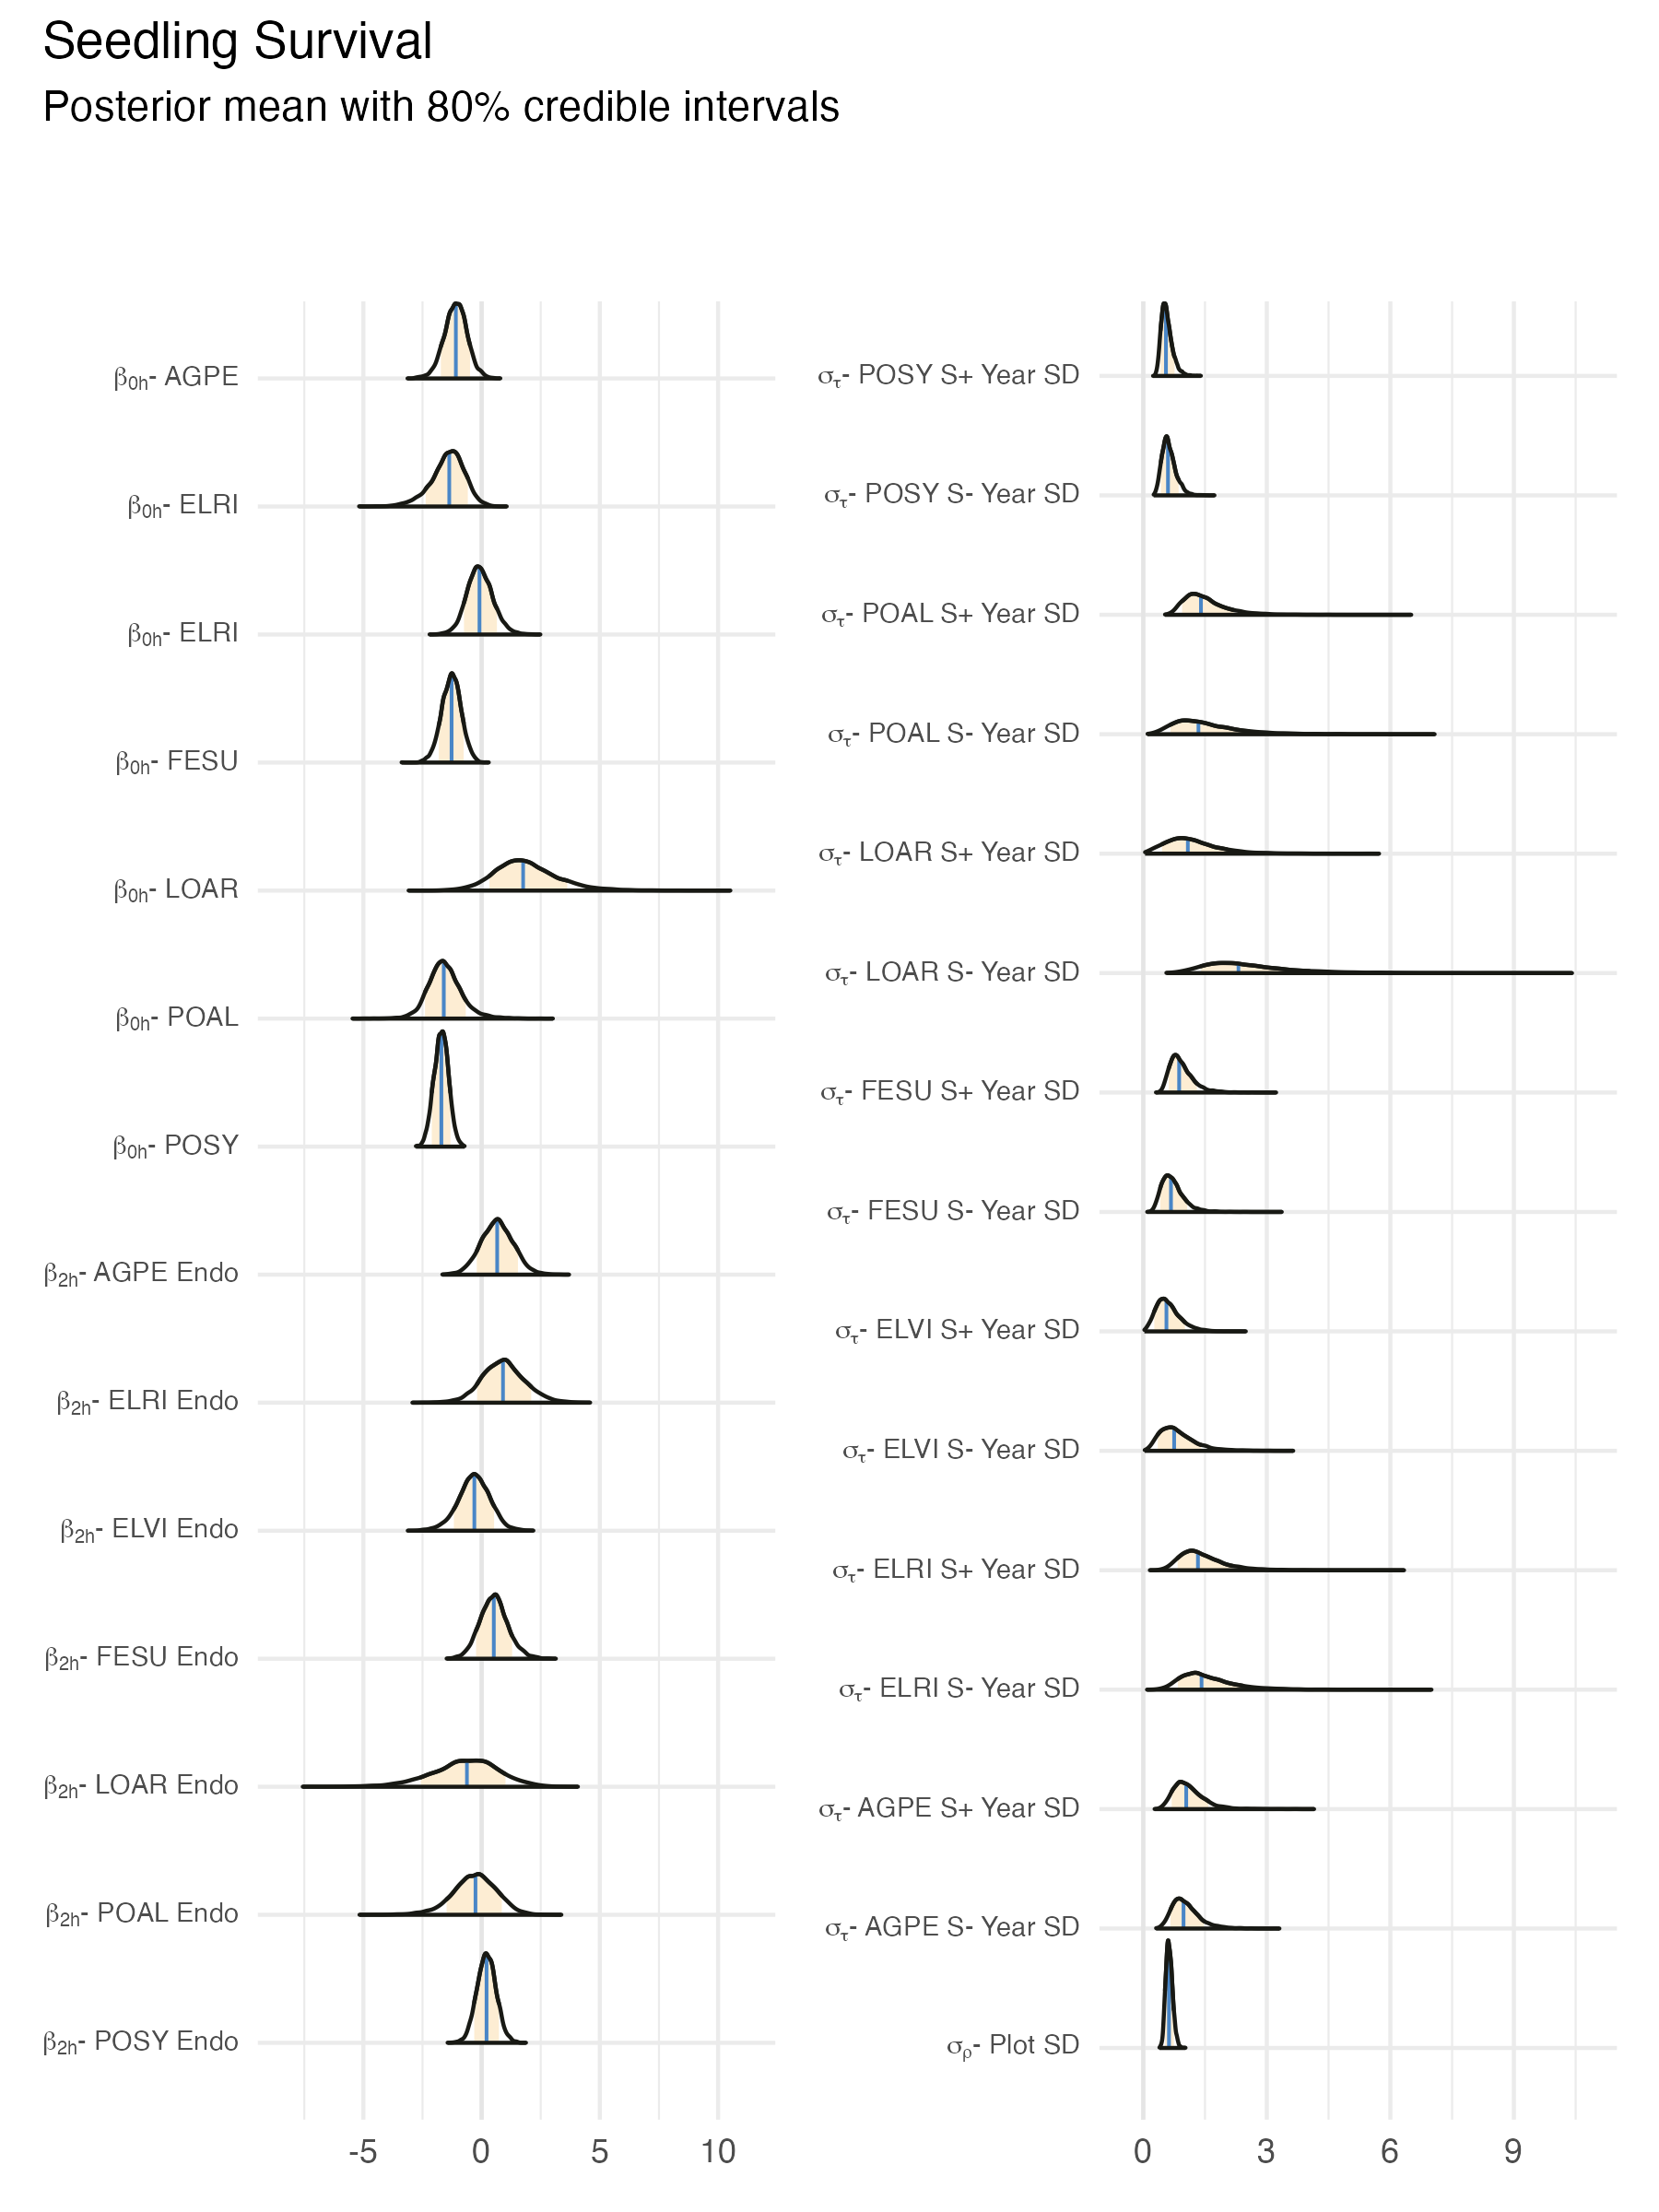
\includegraphics[width = \linewidth]{seedsurv_posteriors_plot.png}
	\caption{Posterior distributions of the vital rate regressions for Seedling Survival. Density curves show $80\%$ credible interval along with the posterior posterior mean.}
\end{figure}

\begin{figure}[H]
	\centering
	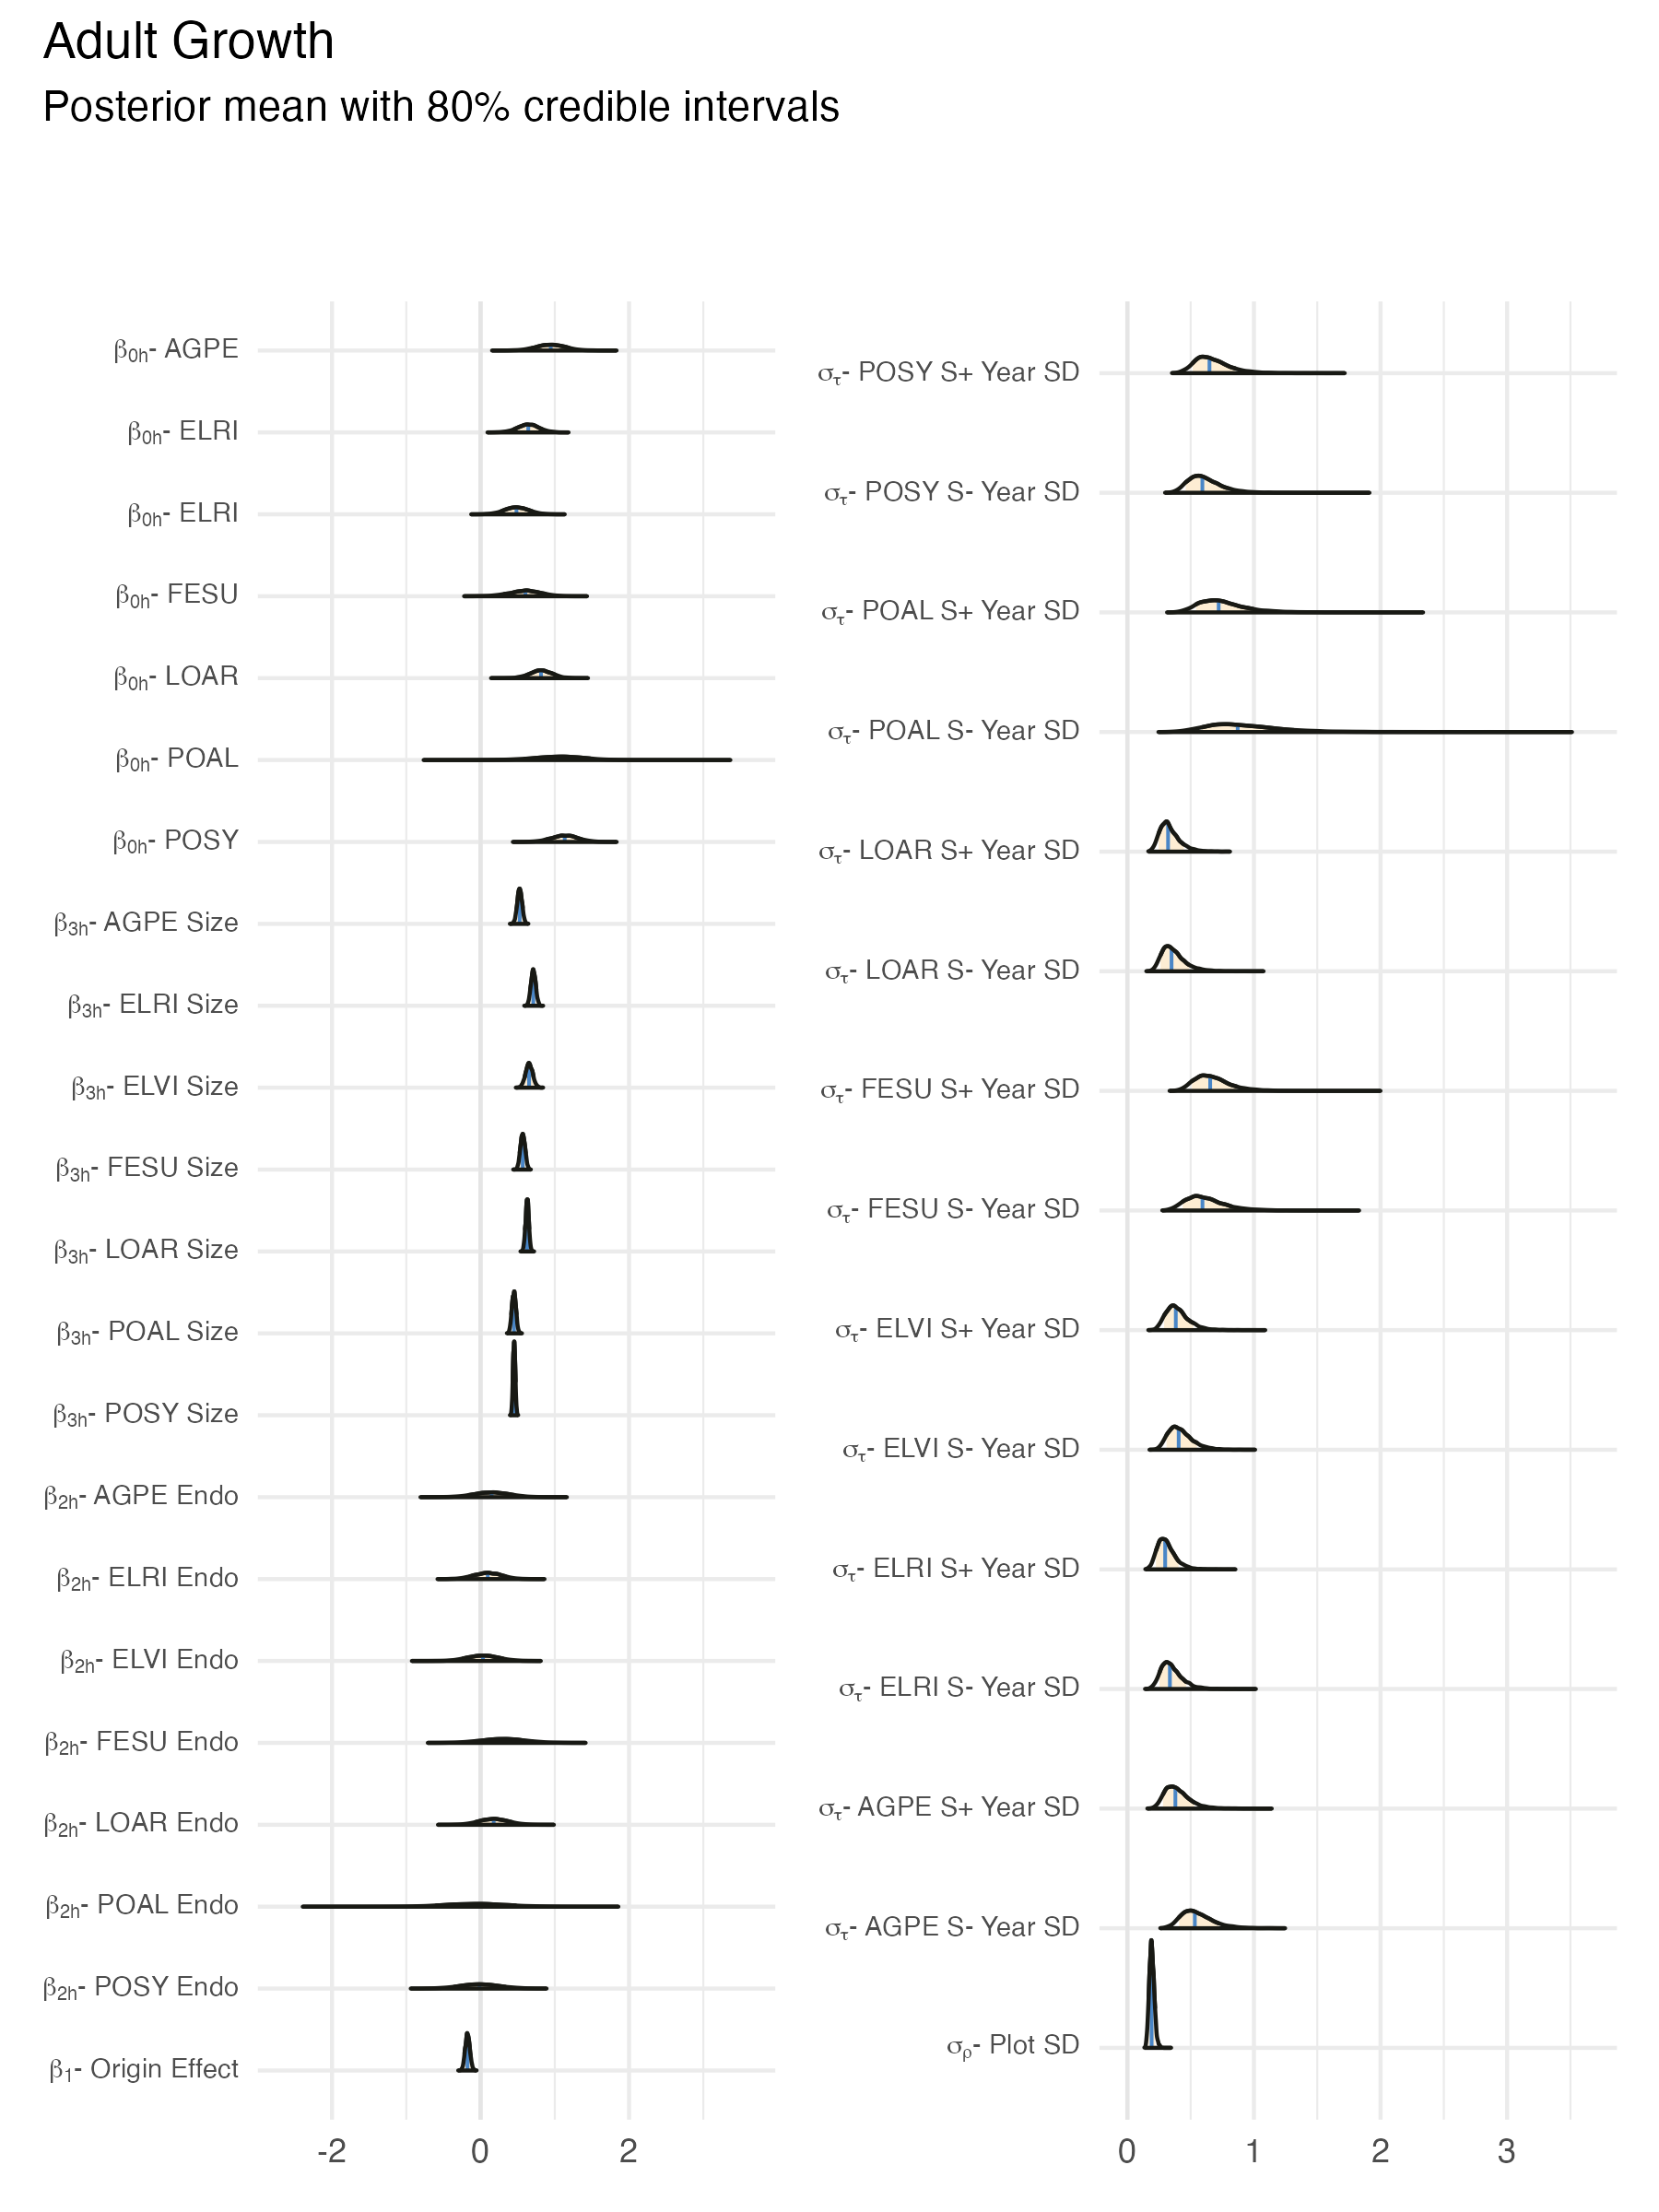
\includegraphics[width = \linewidth]{grow_posteriors_plot.png}
	\caption{Posterior distributions of the vital rate regressions for Adult Growth. Density curves show $80\%$ credible interval along with the posterior posterior mean.}
\end{figure}

\begin{figure}[H]
	\centering
	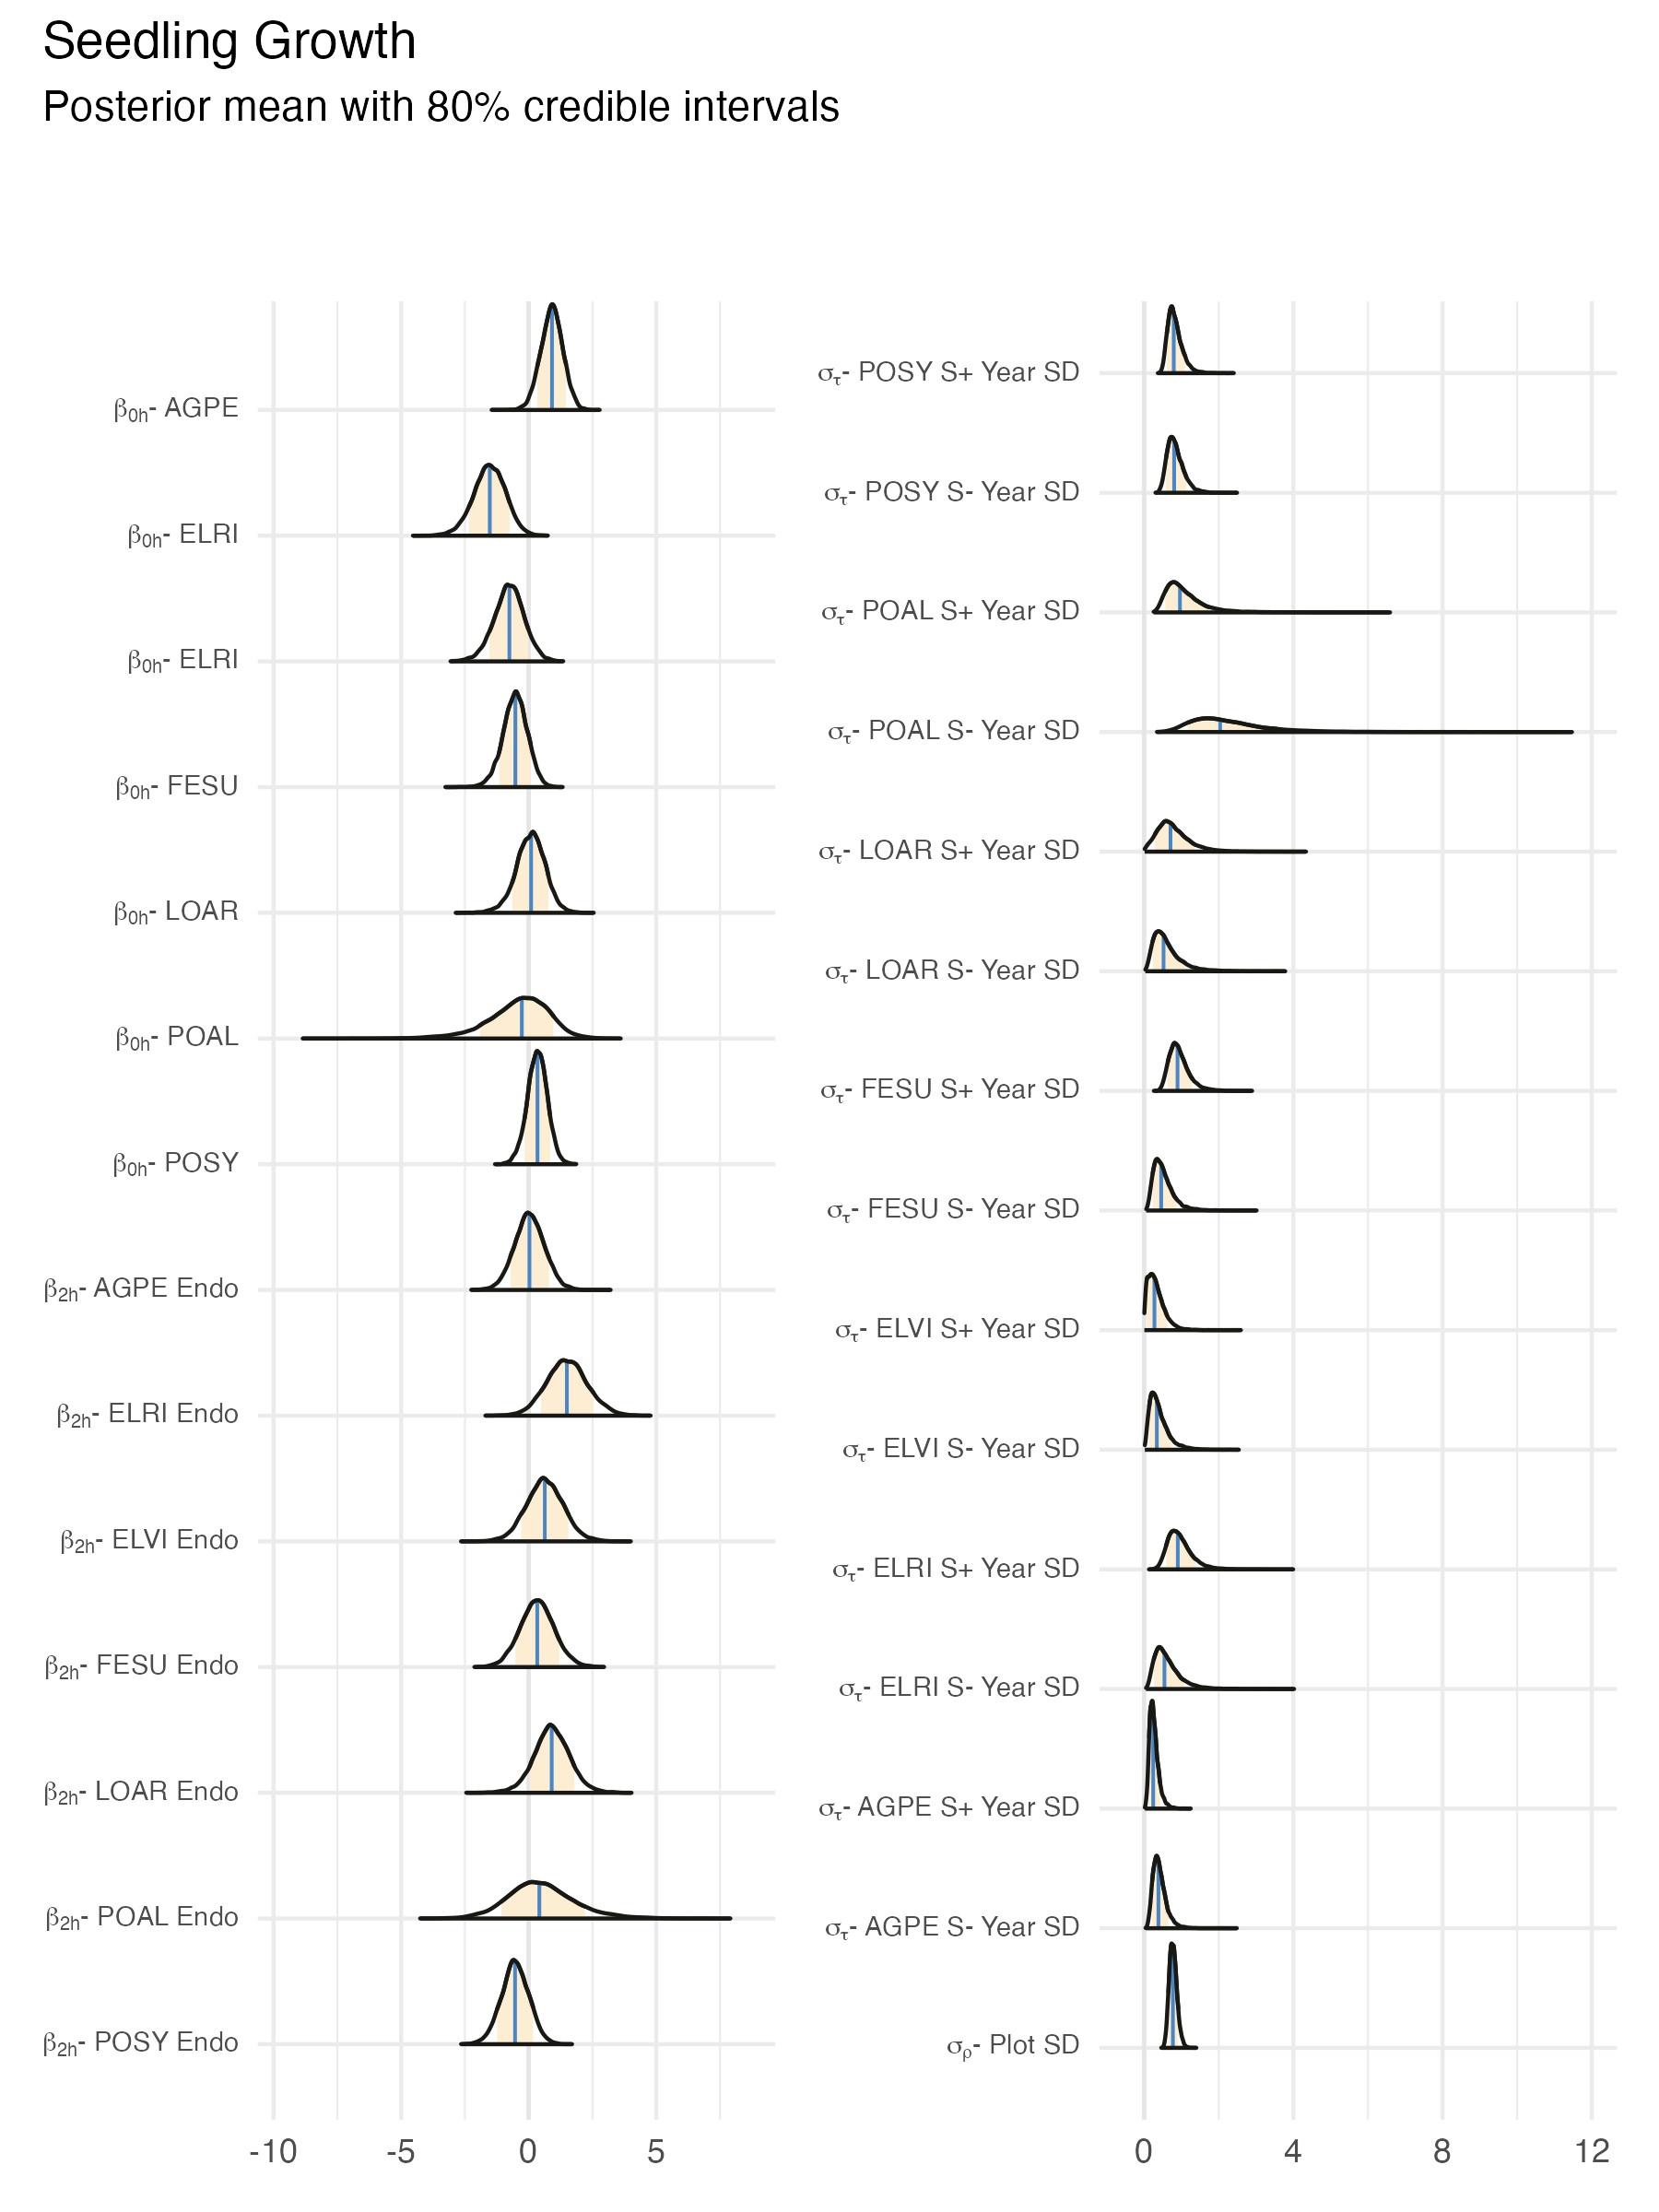
\includegraphics[width = \linewidth]{seedgrow_posteriors_plot.png}
	\caption{Posterior distributions of the vital rate regressions for Seedling Growth. Density curves show $80\%$ credible interval along with the posterior posterior mean.}
\end{figure}


\begin{figure}[H]
	\centering
	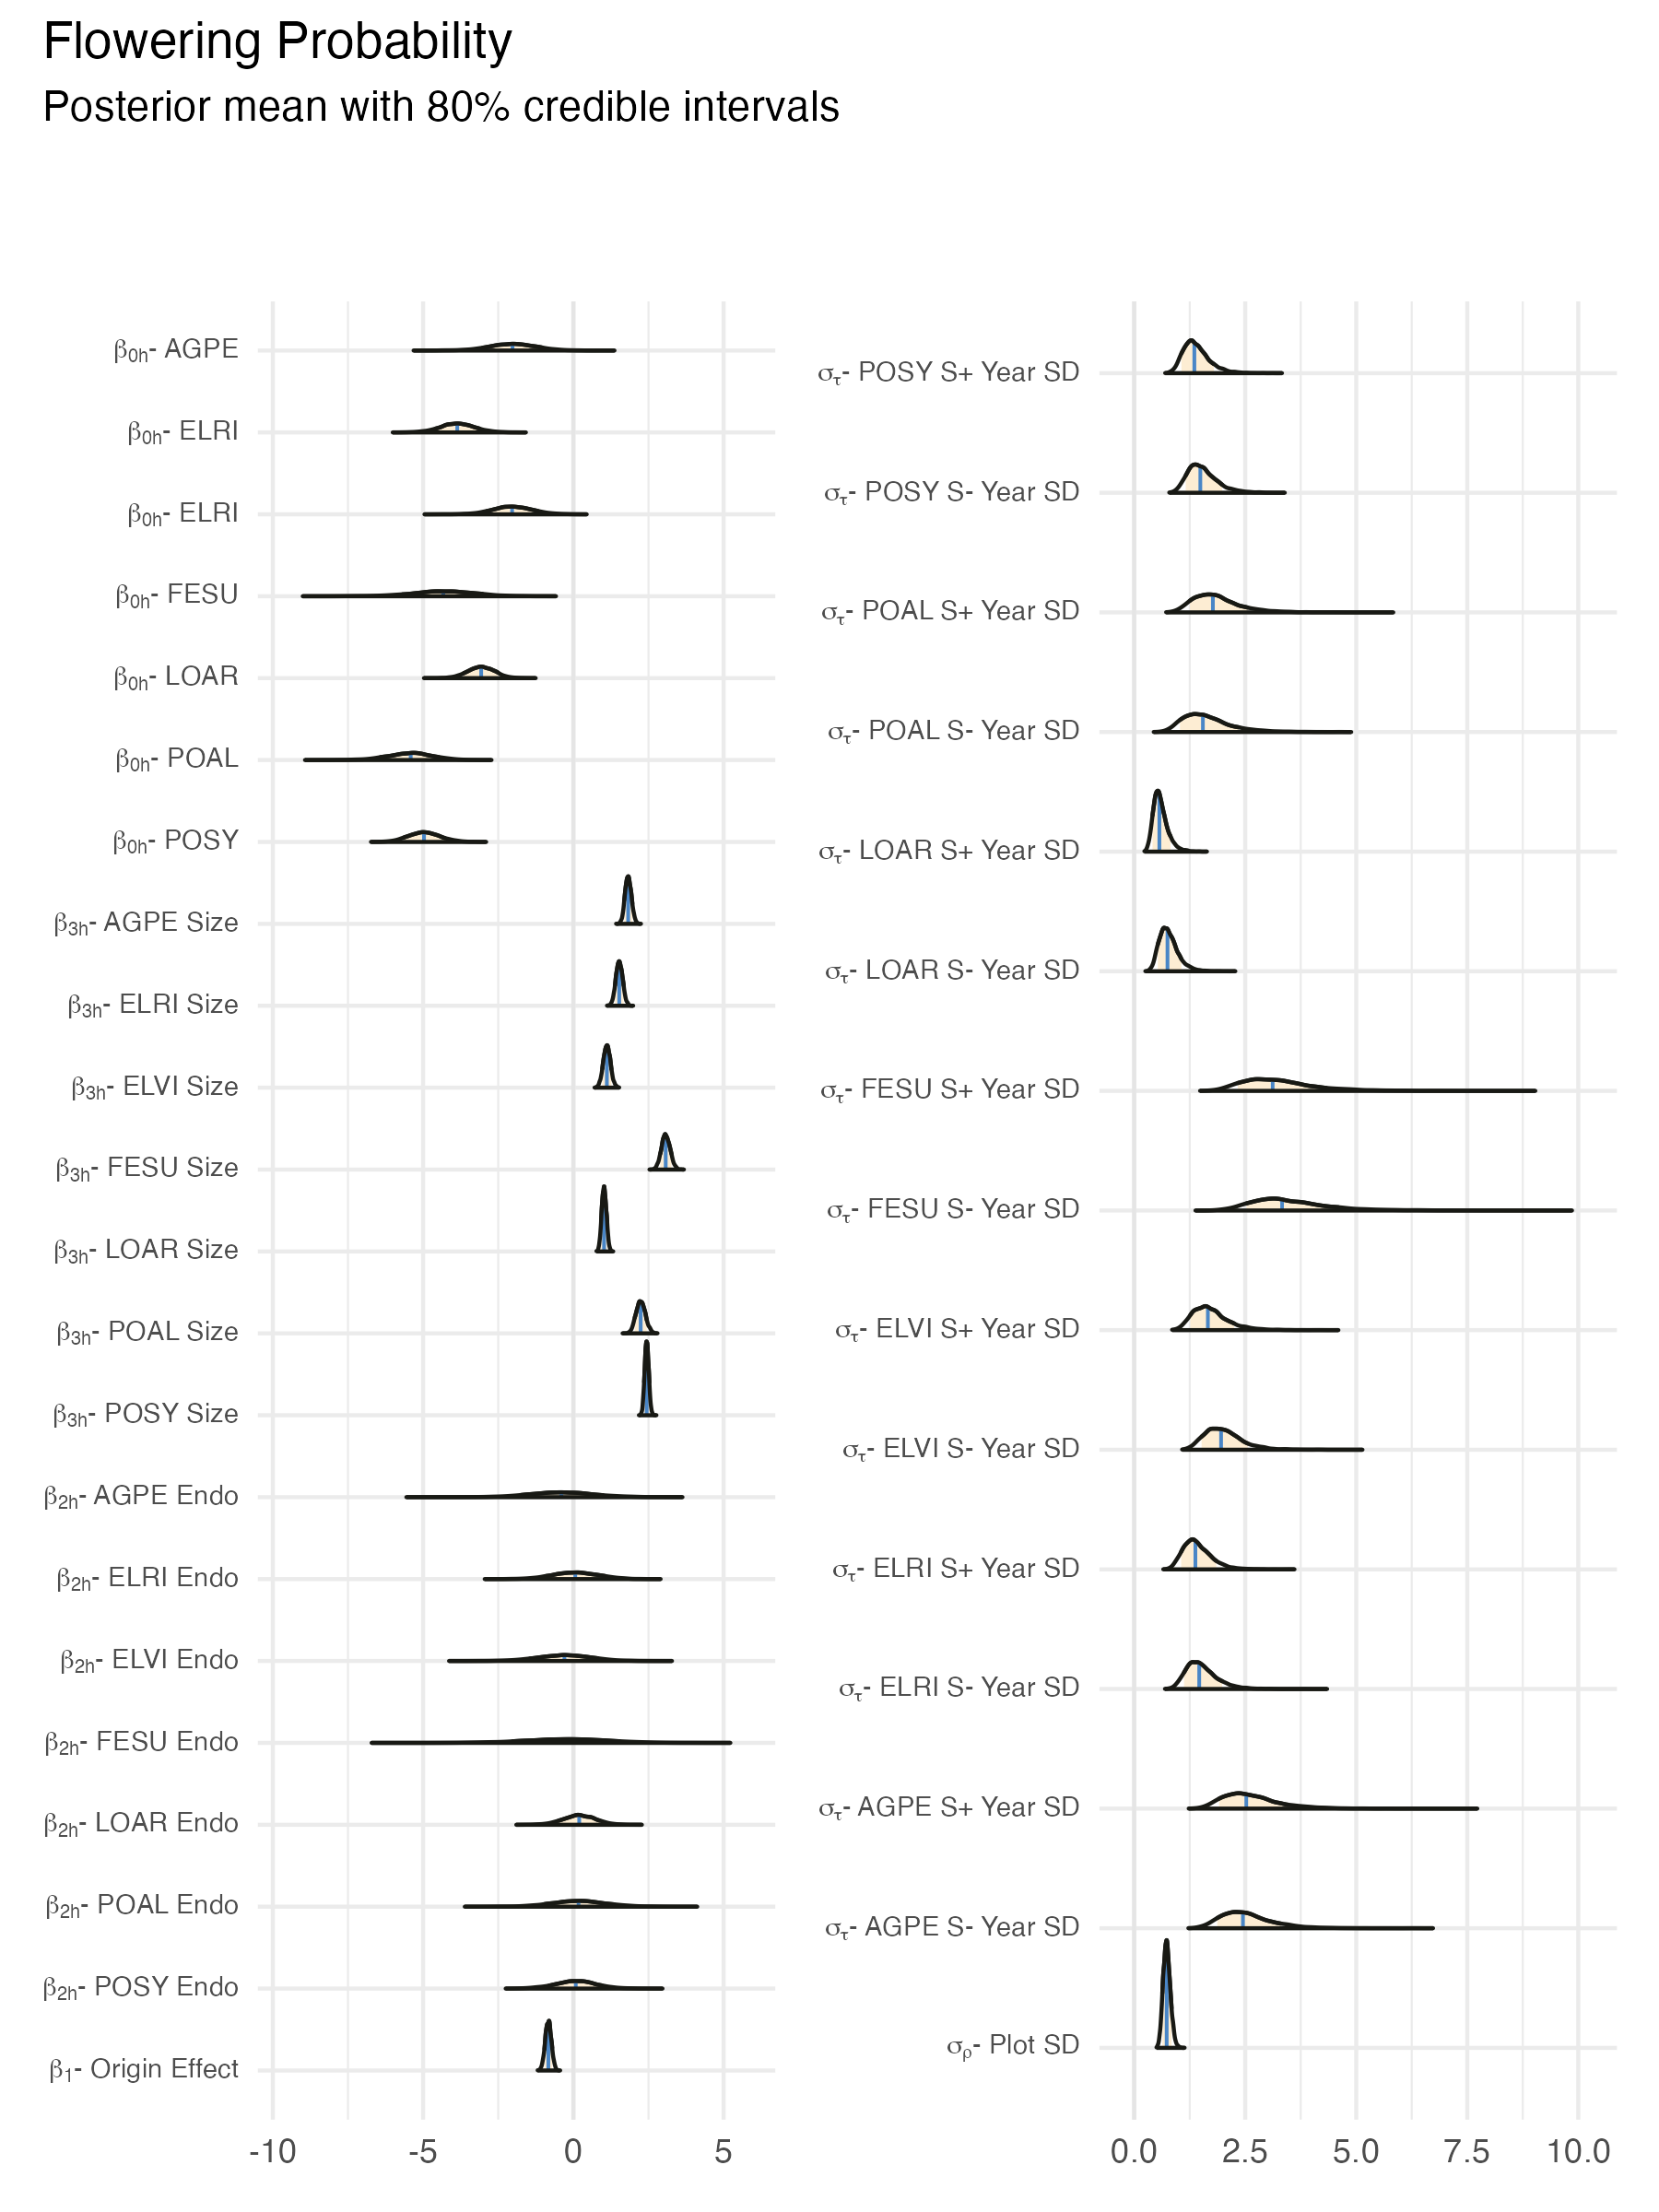
\includegraphics[width = \linewidth]{flw_posteriors_plot.png}
	\caption{Posterior distributions of the vital rate regressions for Flowering Probability. Density curves show $80\%$ credible interval along with the posterior posterior mean.}
\end{figure}


\begin{figure}[H]
	\centering
	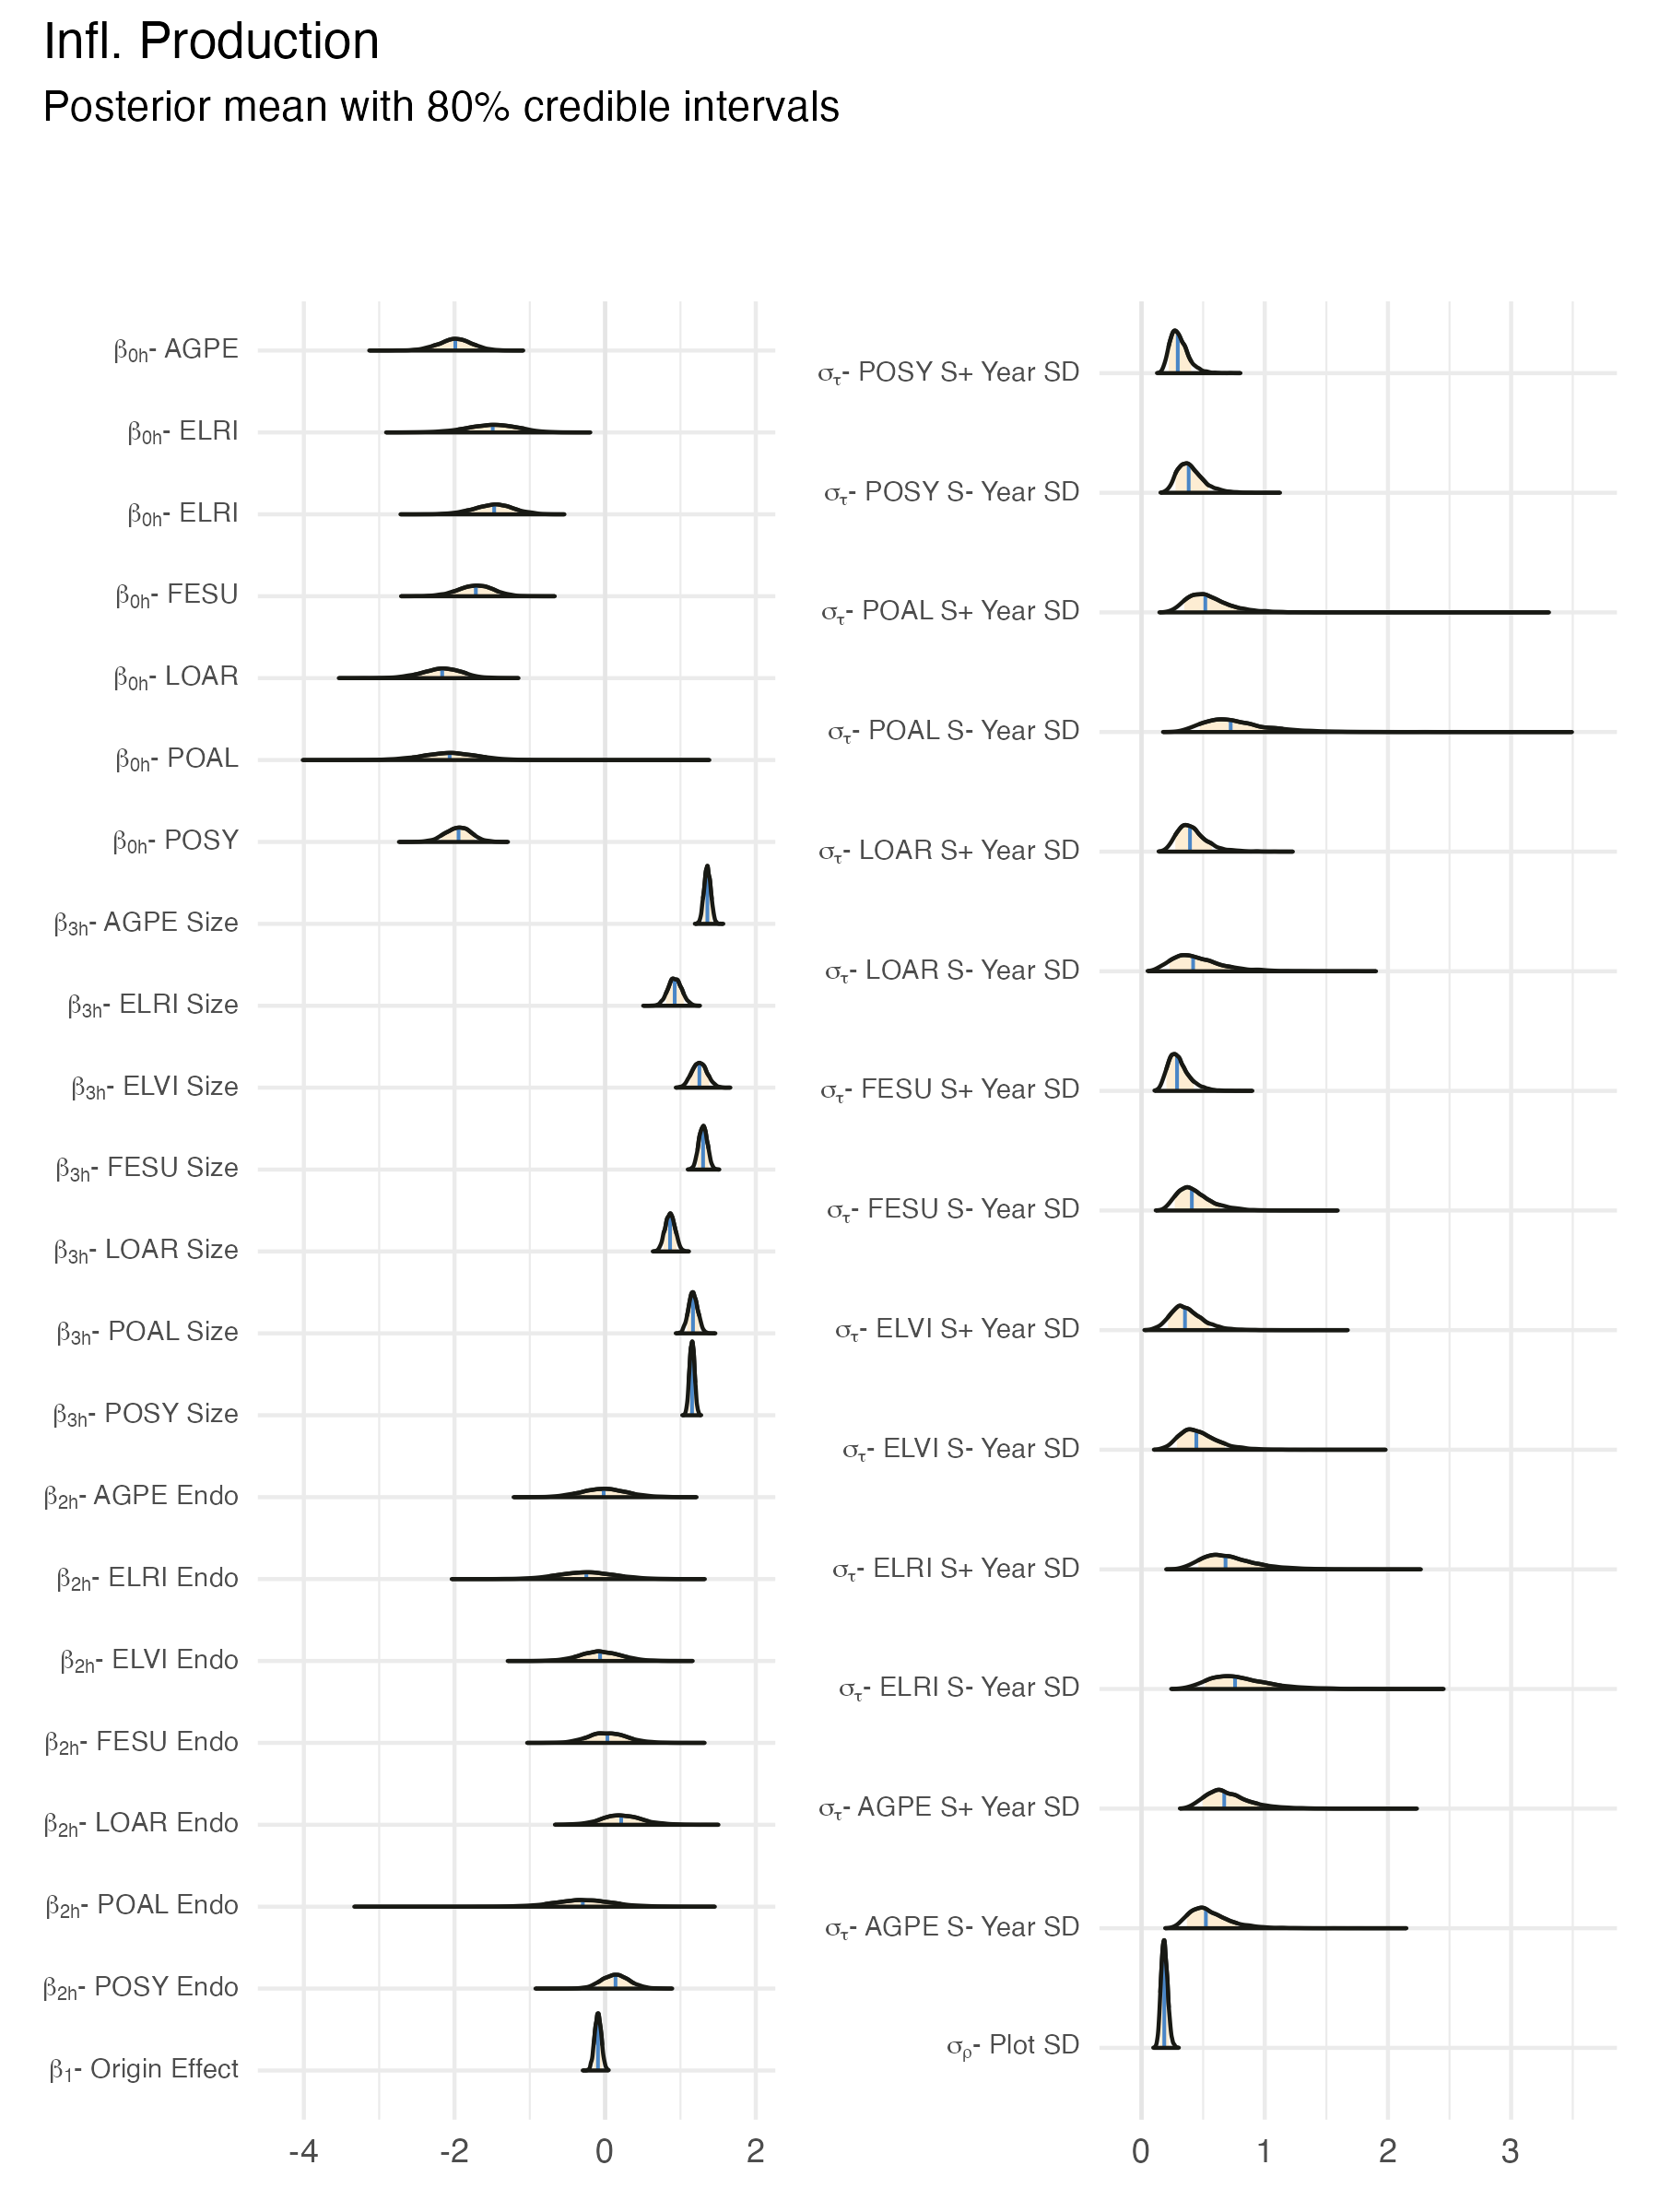
\includegraphics[width = \linewidth]{fert_posteriors_plot.png}
	\caption{Posterior distributions of the vital rate regressions for Inflorescence Production. Density curves show $80\%$ credible interval along with the posterior posterior mean.}
\end{figure}

\begin{figure}[H]
	\centering
	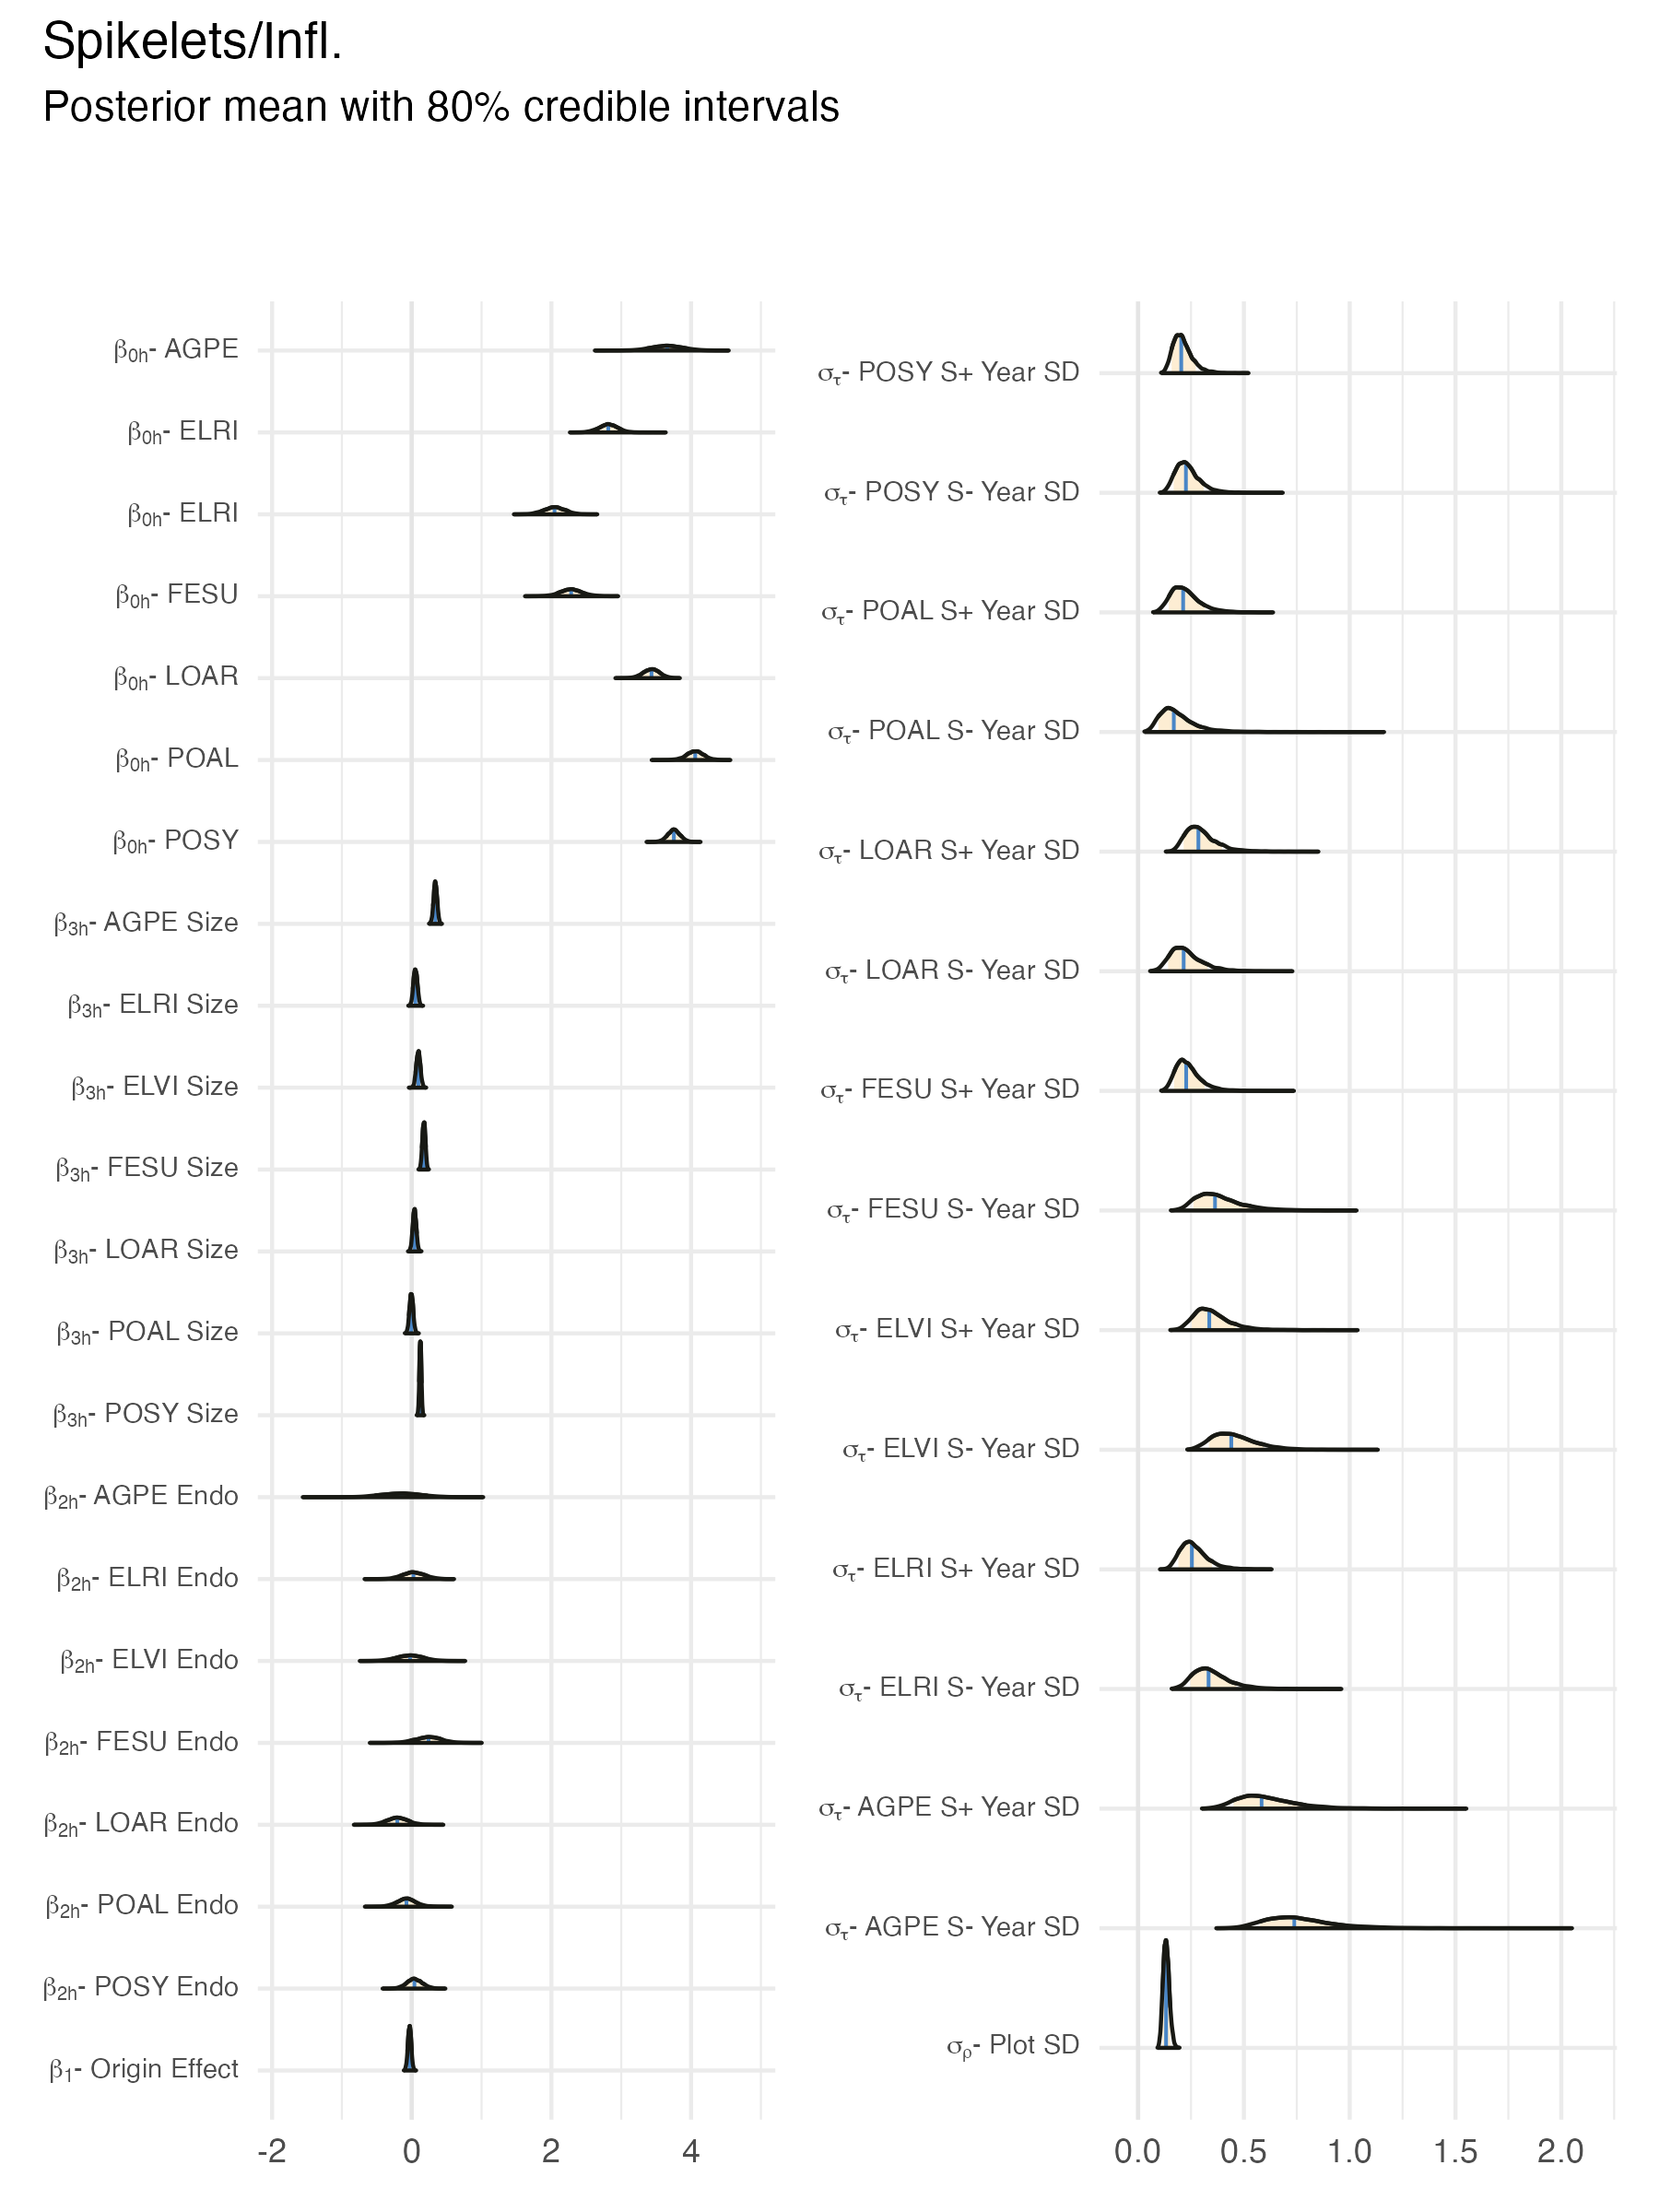
\includegraphics[width = \linewidth]{spike_posteriors_plot.png}
	\caption{Posterior distributions of the vital rate regressions for Spikelets/Inflorescence. Density curves show $80\%$ credible interval along with the posterior posterior mean.}
\end{figure}

\begin{figure}[H]
	\centering
	\includegraphics[width = .8\linewidth]{seedmean_posteriors_plot.png}
	\caption{Posterior distributions of the vital rate regressions for Seeds/Spikelet. Density curves show $80\%$ credible interval along with the posterior posterior mean.}
\end{figure}

\begin{figure}[H]
	\centering
	\includegraphics[width = \linewidth]{stos_posteriors_plot.png}
	\caption{Posterior distributions of the vital rate regressions for Recruitment. Density curves show $80\%$ credible inteinstrval along with the posterior posterior mean.}
\end{figure}


\begin{figure}[H]
	\centering
	\includegraphics[width=\linewidth]{life_cycle_diagram.png}
	\caption{Life cycle graph depicting the generalized structure of matrix population model. Each node represents stages, and arrows represent transitions. Non-reproductive seedlings recruit into the population then transition through size-structured stages (measured as number of tillers). Each species grows to an empirically estimated maximum size (97.5\% of the observed maximum tiller count). Survival and growth transitions are shown in black, and reproduction and recruitment are shown in red. Symbiotic and symbiont-free populations have the same model structure with species-specific and symbiont status-specific transition probabilities used to contruct matrices. Annual vitatl}
\end{figure}

\begin{figure}[H]
	\centering
	\includegraphics[width=\linewidth]{lambda_timeseries_plot.png}
	\caption{Annual growth rate values ($\lambda_{t}$) over thirteen years. Mean values for symbiotic (blue) and symbiont-free (yellow) population growth rates are show along with $80\%$ credible intervals. Dashed line at ($\lambda_{t} = 1$) indicates stable population growth rate. All values are calculated from matrix models representing recruit plants.}
\end{figure}


\begin{figure}[H]
	\centering
	\includegraphics[width=\linewidth]{sim_boxplots.png}
	\caption{(A) Mean and (B) standard deviation of annual growth rate values during simulation scenarios. Each scenario selects from observed transition matrixes, increasing the variance by selecting either all observed years, or a set (6 or 2 years) that have the highest and lowest growth rates for symbiont-free populations.}
\end{figure}


\begin{figure}[H]
	\centering
	\includegraphics[width=\linewidth]{lambdaS_plot.png}
	\caption{Stochastic population growth rates ($\lambda_s$) for symbiotic (blue) and symbiont-free (yellow) populations. Points show posterior medians along with the 95\% credible interval 50\% and posterior medians. All values are calculated from matrix models representing recruit plants.}
\end{figure}




\begin{figure}[H]
	\centering
	\includegraphics[width=\linewidth]{contributions_obs_plot.png}
	\caption{Endophyte contributions to stochastic growth rates under observed and elevated variance across species. The total effect of endophytes (circle) comes from mean benefits (square) and variance buffering (triangle) as well as the interaction between mean and variance effects (diamond). Shapes indicate the posterior mean of each contribution, along with bars for the 50, 75 and 95 \% credible intervals.  Under scenarios of increasing variance, represented by increasing color intensity, effects of variance buffering increase leading to a more mutualistic symbiosis.}
\end{figure}


\begin{figure}[H]
	\centering
	\includegraphics[width=\linewidth]{VRdecomp_contributions_obs_plot.png}
	\caption{Vital rate decomposition of endophyte contributions to stochastic growth rates under observed and elevated variance across species. The total effect of endophytes comes from mean and variance effects across vital rates, but are primarily driver by effect on survival and growth, rather than vital rates associated with reproduction. Circles indicate the posterior mean of each contribution, along with bars for the 50, 75 and 95 \% credible intervals.  Under scenarios of increasing variance, represented by increasing color intensity, effects of variance buffering increase leading to a more mutualistic symbiosis.}
\end{figure}



\begin{figure}[H]
	\centering
	\includegraphics[width=.6\linewidth]{endo_check_plot.png}
	\caption{Faithfulness of experimental plots to assigned endophyte status. Counts of plants scored with leaf peels or seed squashes to check the faithfulness of recruits to the assigned plot-level endophyte status. (A) Endophytic plants may be gained in initially S- plots, or (B) lost in initially S+ plots.}
\end{figure}


\begin{figure}[H]
	\centering
	\includegraphics[width=\linewidth]{climate_plot.png}
	\caption{Weather station time-series for Bloomington, IN. The Seasonal Precipitation-Evapotranspiration Index (SPEI) calculated for the (A) three month growing season and (B) annually from daily weather station observations of (C) average temperatures and (D) cumulative precipitation. Climatic data shown are determined by the census year centered on the month of July.}
\end{figure}


\begin{figure}[H]
	\centering
	\includegraphics[width=.7\linewidth]{spei_combo_lambda_plot.png}
	\caption{Predicted population growth rates across drought indices. Symbiotic (S+; blue) and symbiont-free (S-; tan) populations respond differently to climate as measured by the (A) 3-month SPEI and (B) 12-month SPEI. Thick lines represent the predicted mean growth rate and thin lines show 500 posterior draws.}
\end{figure}

\begin{figure}[H]
	\centering
	\includegraphics[width=\linewidth]{lh_plant_plot.png}
	\caption{Relationship between variance buffering and life history traits describing the fast-slow life history continuum accounting for phylogenetic covariance between grass host species. Regressions between life history traits describing the fast-slow life history continuum ((A) 99th percentile maximum age observed during long term censuses in years; (B) Net reproductive rate; (C) Longevity; (D) Generation time in years; (G) Seed size) and the effect of endophyte symbiosis on the coefficent of variation in population growth rate ($\lambda$). Each panel shows the fitted mean relationship (line) along with the 95\% credible interval.}
\end{figure}


\begin{figure}[H]
	\centering
	\includegraphics[width=\linewidth]{lh_epichloe_plot.png}
	\label{fig:lh_epich}
	\caption{Relationship between variance buffering and life history traits describing the fast-slow life history continuum accounting for phylogenetic covariance between \emph{Epichlo\"{e}} symbionts. Regressions between life history traits describing the fast-slow life history continuum ((A) 99th percentile maximum age observed during long term censuses in years; (B) Net reproductive rate; (C) Longevity; (D) Generation time in years; (G) Seed size) and the effect of endophyte symbiosis on the coefficent of variation in population growth rate ($\lambda$). Results are similar to regressions accounting for host plant phylogeny (Fig. S25), however symbionts are all within a single genus. Each panel shows the fitted mean relationship (line) along with the 95\% credible interval.}
\end{figure}


\begin{figure}[H]
	\centering
	\includegraphics[width=\linewidth]{lh_slopes_plot.png}
	\caption{Posterior estimates of life history trait effects on variance buffering. Grey histograms show the posterior distribution of the slope parameter from models incorporating (A) host plant phylogenetic covariance and (B) symbiont phylogenetic covariance for each life history trait with blue bars showing the posterior mean.}
\end{figure}

\begin{figure}[H]
	\centering
	\includegraphics[width=\linewidth]{lh_allposteriors_plot.png}
	\caption{Posterior distributions of the life history trait regressions. Panels show parameter estimates from phylogenetic models incorporating host phylogenetic covariance (A-G) and for symbiont phylogenetic covariance (H-N). Density curves show $80\%$ credible inteinstrval along with the posterior posterior mean.}
\end{figure}


\newpage

\subsection*{Supplemental Tables S1-S3}
 
\renewcommand\thetable{S\arabic{table}}   

\begin{sidewaystable}\centering
	\caption{Summary of host-endophyte proprogation and transplant methods}
	
	\begin{tabular}{lccc}
		Host Species & Symbiont Species & Heat treatment duration (Temp.)& Transplant date\\
		\midrule
		\emph{Agrostis perennans} & \emph{E. amarillans}&12 min. hot water bath (60 $^{\circ}$C)&April 2008 (10 plots)\\
		\emph{Elymus villosus} &\emph{E. elymi}&6 days drying oven (60 $^{\circ}$C)&April 2008 (10 plots)\\
		\emph{Elymus virginicus} &\emph{E. elymi or EviTG-1}&6 days drying oven (60 $^{\circ}$C)&April 2008 (10 plots)\\
		\emph{Festuca subverticillata} &\emph{E. starrii}&6 days drying oven (60 $^{\circ}$C)&April 2008 (10 plots)\\
		\emph{Lolium arundinaceum} &\emph{E. coenophiala}&6 days drying oven (60 $^{\circ}$C)& Sept. 2007 (10 plots)\\
		\emph{Poa alsodes} &\emph{E. alsodes}& 7 days drying oven (60 $^{\circ}$C)&Sept. 2007 (8 plots)/April 2008 (10 plots)\\
		\emph{Poa sylvestris}&\emph{E. PsyTG-1}&7 days drying oven (60 $^{\circ}$C)& Sept. 2007 (8 plots)/April 2008 (10 plots)\\
		\bottomrule
	\end{tabular}
\end{sidewaystable}

\bigskip

\begin{sidewaystable}\centering
	\caption{Summary of focal life history traits }
	 \setlength{\tabcolsep}{4pt}
	\begin{tabular}{lp{2cm}p{1.7cm}p{1.5cm}p{.8cm}p{1.2cm}p{1.2cm}p{.9cm}p{1.2cm}p{1.5cm}p{1.6cm}}
		
		Host Species &\raggedright Observed max age (years)& \raggedright 99th percentile max age (years)&Generation time (years) & $\mathbf{R}_0$ &Longevity (years)&Seed Length (mm.)&\raggedright Keyfitz Entropy&\raggedright Demetrius Entropy&\raggedright Imperfect transmission rate (\%) & Stromata Observed (\% of indiv. per species)\\
		\midrule
		\emph{Agrostis perennans} &11&7&7.6&0.58&6.4&1.75&0.9&2.1&69.8&0.0\\
		\emph{Elymus villosus} &14&14&20.7&0.35&9.8&7.25&1.3&2.9&100&4.6\\
		\emph{Elymus virginicus} &14&14&13.4&0.25&12.5&8&1.1&2.6&100&0.6\\
		\emph{Festuca subverticillata} &9&6&6.6&0.28&4.3&3.75&0.8&1.8&42.7&0.0\\
		\emph{Lolium arundinaceum} &12$^*$&12$^*$&27.4&0.08&21.3&7&1.1&3.1&100&0.0\\
		\emph{Poa alsodes} &8&6&9.2&0.003&2.6&3.45&0.5&1.2&99.9&0.0\\
		\emph{Poa sylvestris}&12&6&8.0&0.14&3.2&2.6&0.7&1.8&16.6&0.1\\
		\midrule
		\textbf{Pagel's $\lambda$ (host)}&--&0.27&0.28&0.23&0.28&0.27&0.25&0.25&--&--\\
		\textbf{Pagel's $\lambda$ (symbiont)}&--&0.63&0.63&0.63&0.63&0.62&0.62&0.62&--&--\\
		\bottomrule
		
	\end{tabular}
	\raggedright\footnotesize{*Censuses for \emph{L. arundinaceum} plots stopped after year 12 of the experiment.}
\end{sidewaystable}
\bigskip

\begin{sidewaystable}\centering
	\caption{Summary of host-endophyte drought sensitivities}
	\begin{tabular}{lp{1.4cm}p{1.4cm}p{1.5cm}p{1.5cm}p{1.5cm}p{1.5cm}p{1.5cm}p{1.5cm}}
		Host Species& \raggedright Effect on CV($\lambda$)&\raggedright Effect on Mean($\lambda$)&$\frac{\Delta\lambda^{-}}{\Delta SPEI_{3}}$ & $\frac{\Delta\lambda^{+}}{\Delta SPEI_{3}}$ &3 month S- to S+ ratio&$\frac{\Delta\lambda^{-}}{\Delta SPEI_{12}}$ &$\frac{\Delta\lambda^{+}}{\Delta SPEI_{12}}$ & 12 month S- to S+ ratio\\
		\midrule
		\emph{Agrostis perennans} &-0.0264&0.0441&0.03&-0.04&0.85&0.11&-0.06&1.82\\
		\emph{Elymus villosus} &0.0003&0.0509&-0.03&0.01&1.95&0.03&0.04&0.70\\
		\emph{Elymus virginicus} &0.0120&0.0578&0.07&0.05&1.50&0.10&0.07&1.42\\
		\emph{Festuca subverticillata} &-0.0622&0.1639&0.02&0.02&1.01&-0.13&-0.09&1.43\\
		\emph{Lolium arundinaceum} &-0.0118&0.1022&-0.01&0.01&1.32&0.03&-0.03&1.02\\
		\emph{Poa alsodes} &-0.1179&0.1282&0.10&0.14&0.71&0.11&0.14&0.73\\
		\emph{Poa sylvestris}&-0.0298&-0.0085&0.07&0.16&0.44&0.05&0.10&0.55\\
		\bottomrule
	\end{tabular}
\end{sidewaystable}


%%=============================================%%
%% For submissions to Nature Portfolio Journals %%
%% please use the heading ``Extended Data''.   %%
%%=============================================%%

%%=============================================================%%
%% Sample for another appendix section			       %%
%%=============================================================%%

%% \section{Example of another appendix section}\label{secA2}%
%% Appendices may be used for helpful, supporting or essential material that would otherwise 
%% clutter, break up or be distracting to the text. Appendices can consist of sections, figures, 
%% tables and equations etc.

\end{appendices}

%%===========================================================================================%%
%% If you are submitting to one of the Nature Portfolio journals, using the eJP submission   %%
%% system, please include the references within the manuscript file itself. You may do this  %%
%% by copying the reference list from your .bbl file, paste it into the main manuscript .tex %%
%% file, and delete the associated \verb+\bibliography+ commands.                            %%
%%===========================================================================================%%
\newpage

\bibliography{endo_stoch_demo}% common bib file
%% if required, the content of .bbl file can be included here once bbl is generated
%%\input sn-article.bbl


\end{document}
